% Copyright (C) 2014-2025 by Thomas Auzinger <thomas@auzinger.name>

% Inside the square brackets (e.g., [draft,onside]), different options can be chosen:
% 'draft': Obtain debug information on the build.
% 'final': Remove all debug information in the final build.
% 'onside': Create document for onsided printing (without empty pages added by LaTeX).
% 'twoside': Create document for twosided printing, which adds empty pages to start chapters on odd pages.
\documentclass[final,twoside]{vutinfth}

% Define convenience functions to use the author name and the thesis title in the PDF document properties.
%% AIREV [BLOCKER] (The title-page metadata is still the template's: \thesistitle is "Title of the Thesis", the subtitle is the placeholder, \setdate is 01.01.2001, and \Keywords is "a list of keywords". These render on the title pages and in the PDF properties of the submitted document; only you can supply the real title, subtitle or its removal, submission date, and keywords.)
\newcommand{\authorname}{Moritz Jakob Schumacher} % The author name without titles.
\newcommand{\thesistitle}{Title of the Thesis} % The title of the thesis. The English version should be used, if it exists.

% Create the XMP metadata file for the creation of PDF/A compatible documents.
\begin{filecontents*}[overwrite]{\jobname.xmpdata}
\Author{\authorname}                                    % The author's name in the document properties.
\Title{\thesistitle}                                    % The document's title in the document properties.
\Language{en-GB}                                        % The document's language in the document properties. Select 'en-US', 'en-GB', or 'de-AT'.
\Keywords{a\sep list\sep of\sep keywords}               % The document's keywords in the document properties (separated by '\sep ').
\Publisher{TU Wien}                                     % The document's publisher in the document properties.
\Subject{Thesis}                                        % The document's subject in the document properties.
\end{filecontents*}

% Load packages to allow in- and output of non-ASCII characters.
\usepackage{lmodern}        % Use an extension of the original Computer Modern font to minimize the use of bitmapped letters.
\usepackage[T1]{fontenc}    % Determines font encoding of the output. Font packages have to be included before this line.
\usepackage[utf8]{inputenc} % Determines encoding of the input. All input files have to use UTF8 encoding.

% Usepackages for the fisuals in the design chapter
\usepackage{tikz}
\usetikzlibrary{arrows.meta, positioning, calc}
\usepackage{xcolor}

\definecolor{subjectblue}{RGB}{59,130,246}
\definecolor{subjectblue20}{RGB}{219,234,254}
\definecolor{subjectgreen}{RGB}{16,185,129}
\definecolor{subjectgreen20}{RGB}{209,250,229}
\definecolor{subjectorange}{RGB}{245,158,11}
\definecolor{subjectorange20}{RGB}{254,243,199}
\definecolor{plannedfill}{RGB}{229,231,235}
\definecolor{panelgray}{RGB}{247,247,247}
\definecolor{doneborder}{RGB}{156,163,175}
\definecolor{donefill}{RGB}{243,244,246}

% Extended LaTeX functionality is enables by including packages with \usepackage{...}.
\usepackage{amsmath}    % Extended typesetting of mathematical expression.
\usepackage{amssymb}    % Provides a multitude of mathematical symbols.
\usepackage{mathtools}  % Further extensions of mathematical typesetting.
\usepackage{microtype}  % Small-scale typographic enhancements.
\usepackage{csquotes}   % Provides \enquote for context-sensitive quotation marks (used in Related Work).
\usepackage[inline]{enumitem} % User control over the layout of lists (itemize, enumerate, description).
\usepackage{multirow}   % Allows table elements to span several rows.
\usepackage{booktabs}   % Improves the typesetting of tables.
\usepackage{longtable}  % Allows tables to span multiple pages.
\usepackage{subcaption} % Allows the use of subfigures and enables their referencing.
\usepackage[ruled,linesnumbered,algochapter]{algorithm2e} % Enables the writing of pseudo code.
\usepackage[dvipsnames,table]{xcolor} % Allows the definition and use of colors. This package has to be included before tikz.
\usepackage{nag}        % Issues warnings when best practices in writing LaTeX documents are violated.
\usepackage{todonotes}  % Provides tooltip-like todo notes.
\usepackage{morewrites} % Increases the number of external files that can be used.
\usepackage[a-2b,mathxmp]{pdfx}      % Enables PDF/A compliance. Loads the package hyperref and has to be included second to last.
\usepackage[acronym,toc]{glossaries} % Enables the generation of glossaries and lists of acronyms. This package has to be included last.

% Preamble for appendix
% Required packages:
\usepackage{longtable,booktabs,array,ragged2e}
\usepackage{enumitem}
\setlist[itemize]{leftmargin=*,nosep}

% Set PDF document properties
\hypersetup{
    pdfpagelayout   = TwoPageRight,           % How the document is shown in PDF viewers (optional).
    linkbordercolor = {Melon},                % The color of the borders of boxes around hyperlinks (optional).
}

\setpnumwidth{2.5em}        % Avoid overfull hboxes in the table of contents (see memoir manual).
\setsecnumdepth{subsection} % Enumerate subsections.

\nonzeroparskip             % Create space between paragraphs (optional).
\setlength{\parindent}{0pt} % Remove paragraph indentation (optional).

\makeindex      % Use an optional index.
\makeglossaries % Use an optional glossary.
%\glstocfalse   % Remove the glossaries from the table of contents.

% Set persons with 4 arguments:
%  {title before name}{name}{title after name}{gender}
%  where both titles are optional (i.e. can be given as empty brackets {}).
\setauthor{}{Moritz Jakob Schumacher}{B.Sc.}{male}
\setadvisor{Assistant Prof. Dr.rer.nat.}{René Röpke}{B.Sc. M.Sc.}{male}

% For bachelor and master theses:
\setfirstassistant{}{Selina Reinhard}{B.Sc. M.Sc.}{female}
%\setsecondassistant{Pretitle}{Forename Surname}{Posttitle}{male}
%\setthirdassistant{Pretitle}{Forename Surname}{Posttitle}{male}

% For dissertations:
%\setfirstreviewer{Pretitle}{Forename Surname}{Posttitle}{male}
%\setsecondreviewer{Pretitle}{Forename Surname}{Posttitle}{male}

% For dissertations at the PhD School and optionally for dissertations:
%\setsecondadvisor{Pretitle}{Forename Surname}{Posttitle}{male} % Comment to remove.

% Required data.
\setregnumber{12331473}
\setdate{01}{01}{2001} % Set date with 3 arguments: {day}{month}{year}.
\settitle{\thesistitle}{Titel der Arbeit} % Sets English and German version of the title (both can be English or German). If your title contains commas, enclose it with additional curvy brackets (i.e., {{your title}}) or define it as a macro as done with \thesistitle.
\setsubtitle{Optional Subtitle of the Thesis}{Optionaler Untertitel der Arbeit} % Sets English and German version of the subtitle (both can be English or German).

% Select the thesis type: bachelor / master / doctor.
% Bachelor:
%\setthesis{bachelor}
%
% Master:
\setthesis{master}
\setmasterdegree{dipl.} % dipl. / rer.nat. / rer.soc.oec. / master
%
% Doctor:
%\setthesis{doctor}
%\setdoctordegree{rer.soc.oec.}% rer.nat. / techn. / rer.soc.oec.

% For bachelor and master:
\setcurriculum{Software Engineering}{Software Engineering} % Sets the English and German name of the curriculum.

% Optional reviewer data:
%\setfirstreviewerdata{Affiliation, Country}
%\setsecondreviewerdata{Affiliation, Country}


\begin{document}

\frontmatter % Switches to roman numbering.
% The structure of the thesis has to conform to the guidelines at
%  https://informatics.tuwien.ac.at/study-services

\addtitlepage{naustrian} % German title page.
\addtitlepage{english} % English title page.
\addstatementpage{naustrian}  % Select 'english' for the English statement text.

\begin{danksagung*}
Ein großes Dankeschön geht an meinen Betreuer, Assistant Prof. Dr. rer. nat. René Röpke, für die engagierte Begleitung dieser Arbeit. Ebenso herzlich danke ich Selina Reinhard für das geduldige Mitlesen, während diese Arbeit Stück für Stück Gestalt annahm.

Mein besonderer Dank gilt den Studierenden, die an den beiden Studien teilgenommen und mir ihre Zeit geschenkt haben. Auf ihren Erfahrungen und ehrlichen Rückmeldungen baut diese gesamte Arbeit auf.

Zu guter Letzt danke ich meiner Familie sowie meinen Freundinnen und Freunden von Herzen für die Unterstützung und Geduld während meines gesamten Studiums.
\end{danksagung*}

\begin{acknowledgements*}
A big thank you goes to my supervisor, Assistant Prof. Dr. rer. nat. René Röpke, for his dedicated guidance throughout this thesis. I also warmly thank Selina Reinhard for her patient proofreading as this work gradually took shape.

My special thanks go to the students who participated in both studies and generously gave their time. This entire work is built upon their experiences and honest feedback.

Finally, I thank my family and friends from the bottom of my heart for their support and patience throughout my entire studies.
\end{acknowledgements*}

\begin{kurzfassung}
Studierende planen ihr Studium anhand von Curricula, die Voraussetzungen,
Wahlmöglichkeiten und institutionelle Regeln festlegen. Die Werkzeuge, die diese
Planung unterstützen, sind zweigeteilt. Graphbasierte Systeme stellen die
Struktur eines Curriculums dar, lassen jedoch den zeitlichen Ablauf außen vor;
tabellenbasierte Planungswerkzeuge verteilen Lehrveranstaltungen auf Semester
und prüfen das Ergebnis gegen die Studienordnung, lassen aber die Struktur
implizit. Wo beides in einem Werkzeug zusammengeführt wurde, ist die
Abhängigkeitsinformation in den Zeitplan selbst eingebettet und damit an eine
chronologische Anordnung gebunden.

Diese Arbeit entwirft, implementiert und evaluiert eine hybride
Graph-Tabellen-Oberfläche, in der ein navigierbarer Curriculumsgraph und eine
semesterorientierte Tabelle auf einen gemeinsamen Plan schreiben. Die
Anforderungen stehen am Anfang: Eine formative Studie mit sechs Studierenden,
durchgeführt anhand eines interaktiven, aber nicht funktionsfähigen Prototyps,
ergibt eine gereihte Spezifikation von 13 Features mit 55 nummerierten
Anforderungen. Das Werkzeug wird anschließend mit elf Studierenden evaluiert,
die jeweils einmal ohne und einmal mit der Graphansicht planen und dabei über
eine bildweise Aufzeichnung der Oberfläche, ein Think-aloud-Transkript und
Fragebögen nach den Aufgaben beobachtet werden.

Eine explorative Evaluierung mit elf Studierenden zeigte eine durchgängige, von
einer Checkliste getriebene Planungsschleife über alle Erfahrungsstufen hinweg.
Der Graph trat bei der Suche nach Kandidaten an die Stelle des
Lehrveranstaltungskatalogs, während Lehrveranstaltungen weiterhin in der Tabelle
festgelegt wurden. Dieser geteilte Arbeitsablauf machte eine Parking Stage als
Puffer für noch nicht festgelegte Lehrveranstaltungen zwischen den beiden
Ansichten unverzichtbar. Da das Curriculum zudem nur wenige strikte
Abhängigkeiten festlegt, verschob sich der wesentliche Nutzen des Graphen vom
Abbilden von Reihenfolgen hin zur Orientierung und zum gefilterten Erkunden. Die
berichtete Zufriedenheit war insgesamt hoch, wobei die schwächste Skala
(Perspicuity) genau mit den Terminologieschwierigkeiten übereinstimmt, die
während der Aufgaben beobachtet wurden.

\end{kurzfassung}

\begin{abstract}
Students in higher education plan their studies against curricula that encode
prerequisites, electives and institutional rules, and the tools available to
them are split. Graph-based systems draw the structure of a curriculum but
leave the timeline aside; table-based planners arrange courses across semesters
and check the result against the regulations, but leave the structure implicit.
Where both have been brought into one tool, dependency information has been
embedded in the schedule itself, which ties it to a chronological layout.

This thesis designs, builds and evaluates a hybrid graph--table interface in
which a browsable curriculum graph and a schedule-managing table write to one
shared plan. The work proceeds in three steps. A formative study with six
students of two TU~Wien Informatics programmes, conducted around an interactive
but non-functional prototype, yields 64 themes that are translated into a ranked
specification of 13 features carrying 55 numbered requirements. From that
specification the tool is designed and implemented: a Graph View that draws the
curriculum as its containment hierarchy with formal prerequisites as a
switchable overlay, a Table View holding the same plan as semester lanes, a
Compliance Engine that checks the plan against two degree regulations after
every change, and a Recommendation Panel whose suggestions carry an explanation.
The tool is then evaluated with eleven students, each planning once without the
Graph View and once with it, observed through a frame-sampled record of the
interface rather than through self-report alone.

Planning took the shape of a single checklist-driven loop, the same for the most
fluent and the most junior participants. The graph did not extend that loop: it
took the place of the course catalogue at the step where candidates are found,
while courses continued to be committed in the table, and the period of the loop
was unchanged. Measuring the plans against their brief rather than against what
students reported revealed a calibration gap: every participant reported success
in runs where no plan met its brief and the tool reported nothing missing.

The evidence is descriptive. Two small samples at one institution, a fixed
scenario order, a single coder and descriptive statistics support an account of
how these students planned, not a claim that a component caused a behaviour.
What the work offers is a requirements specification traceable to student
evidence, a working artefact whose design decisions are recorded with their
costs, and a process-level account of planning with such a tool.

\end{abstract}

% Select the language of the thesis, e.g., english or naustrian.
\selectlanguage{english}

% Add a table of contents (toc).
\tableofcontents % Starred version, i.e., \tableofcontents*, removes the self-entry.

% Switch to arabic numbering and start the enumeration of chapters in the table of content.
\mainmatter

\chapter{Introduction}
%% AIREV [MINOR] (Document-wide residual: "dependency" is used in two senses, the containment relation the graph draws and the prerequisite relation of the cited literature, and about forty occurrences have not been checked against the glossary definition proposed at the end of the glossary. After the Introduction, Related Work and glossary edits are made, sweep every "dependenc*" occurrence and confirm each is either the prerequisite sense or an explicit historical description of the prototype and the formative interviews.)
\label{chap:introduction}
Students in higher education face growing challenges in planning their studies. Curricula involve complex prerequisites, electives, and institutional rules that students must reconcile. While institutions publish exemplary study plans, these assume an idealised progression; a single failed examination or postponed module immediately necessitates an individualised schedule~\cite{judel_supporting_2023}. Varying study speeds and limited access to guidance compound this issue. Advisors struggle to provide evidence-based scheduling advice at scale~\cite{schulte_large_2017}, which is critical given that the timing and sequencing of courses are associated with time to degree, and less strongly with final grade~\cite{morsy_study_2019}.

Existing approaches address these issues but remain limited. Graph-based systems focus mainly on visualising curriculum structure and the \gterm{dependency}{dependencies} it encodes~\cite{auvinen_stops_2014, rollande_graph_2013, trippel_developing_2025}, while table-based planning tools emphasise semester-level scheduling~\cite{hirmer_requirements_2022, judel_supporting_2023, srisamutr_course_2018}; where both appear in one tool, the dependency view stays local to a single module. This motivates investigating a hybrid approach: integrating a graph and a table into a single planning workflow so students can understand structure and dependencies (graph) and manage their schedule and workload (table).
Two further strands turn student data into feedback. Educational Dashboards (ED) report a student's standing~\cite{schwendimann2017, verbert_learning_2020, loboda_mastery_2014}, while Educational Recommender Systems (ERS) suggest which courses to take next~\cite{bhumichitr_recommender_2017, esteban_helping_2020, al-badarenah_automated_2016}. Both are well established, and both are almost always built separately~\cite{bodily_review_2017}. How the two should be combined within a student's own planning workflow therefore remains open. This thesis puts that question to students, in the formative study of Chapter~\ref{chap:formative-study}, and derives the answer from what they report.

\section{Research Questions}
\label{sec:research-questions}

Building on the challenges and gaps outlined above, this thesis investigates the design, implementation, and use of a hybrid graph-table study planner, built for and evaluated against two degree programmes at the Faculty of Informatics of the Vienna University of Technology (TU~Wien): the Bachelor programme in Computer Science\footnote{\url{https://informatics.tuwien.ac.at/bachelor/curriculum-ue033521.pdf}} and the Master programme in Software Engineering\footnote{\url{https://informatics.tuwien.ac.at/master/curriculum-ue066937.pdf}}. We formulate three research questions:

\textbf{Research Question 1} \emph{What are students' needs and resulting requirements for a hybrid graph-table interface that supports programme-level study planning and understanding of curriculum structure and course dependencies?}

This question is addressed by the formative study, conducted with an interactive but non-functional prototype (Chapter~\ref{chap:formative-study}), whose findings are translated into a ranked features-and-requirements specification in the same chapter (Section~\ref{chap:from-themes-to-requirements}).
Building on these requirements, the second sub-question concerns the design and construction of the tool itself:

\textbf{Research Question 2} \emph{How can we design and implement a hybrid interface that combines graph-based visualisation with table-based planning to help students plan their studies and understand curriculum structure and course dependencies, based on those requirements?}

This question is addressed by the Design chapter (Chapter~\ref{chap:design}), which derives each design decision from a requirement, prior evidence, or an explicitly stated assumption, and by the Implementation chapter (Chapter~\ref{chap:implementation}), which realises that design as a working system.
Finally, the third question asks how the implemented system is used by the students it was built for, and what its graph contributes to that use:

\textbf{Research Question 3} \emph{How do students plan with the hybrid interface, and what does the graph-based view contribute to their planning?}

The evaluation reads this question through three lenses: the planning process as the recordings show it, the plans students produce, measured against their brief and against what students and the tool report as complete, and the satisfaction students report. This question is addressed by an evaluation study with students (Chapter~\ref{chap:evaluation}), interpreted in the Discussion (Chapter~\ref{chap:discussion}) and answered in the Conclusion (Chapter~\ref{chap:conclusion}).

\section{Contributions}
\label{sec:contributions}

This thesis makes the following contributions:

\TDrev{Re-check the contributions once Evaluation and Discussion are final}{Kept open at your request. Contribution one now states the specification's size, and contributions three and four track Chapter~\ref{chap:evaluation}'s two headline results. One thing to settle when Chapters~\ref{chap:evaluation} and~\ref{chap:discussion} are closed: contribution two says the tool \enquote{embeds explainable recommendations}, which is true of what was designed, built and evaluated: all six families were live during the sessions (settled 2026-09-05; Chapter~\ref{chap:implementation}, Section~\ref{sec:impl-recommender}). What the study cannot speak to is the quality of the suggestions, which OOS5 already places out of scope, so the contribution needs no narrowing on that account.}
\begin{itemize}
    \item \textbf{A requirements specification for study planning.} A ranked specification of 13 features carrying 55 numbered requirements for a study-planning tool, each traceable through a theme to the formative interview evidence that motivated it (Section~\ref{chap:from-themes-to-requirements}).
    \item \textbf{A hybrid graph-table planning tool.} The design and implementation of a web-based tool that unites a curriculum graph and a schedule-managing table over a single shared plan, checks that plan against the regulations of two degree programmes in real time, and embeds explainable recommendations within the planning workflow (Chapters~\ref{chap:design}--\ref{chap:implementation}).
    \item \textbf{An account of what a curriculum graph contributes to planning.} Evidence, from a within-subjects study of eleven students observed at the level of the interface itself, that the graph enters the planning process at one point: it replaces the Course Catalogue as the surface on which a named gap is turned into candidate courses, and it leaves untouched the step at which a course is committed to a semester, because it renders no semester dimension against which that commitment could be judged (Chapter~\ref{chap:evaluation}).
    \item \textbf{Evidence that a completion signal students trust can certify a plan it has not checked.} Plans that missed their brief were reported as successes by the students who produced them, and the tool agreed, because the constraints it does not model are silent rather than wrong. This bears on any planning tool that guides through a checklist (Chapter~\ref{chap:evaluation}).
\end{itemize}

The last two contributions rest on two records. The account of how students planned is read from a frame-sampled log of the interface state; the catalogue of usability problems and positive findings is coded from that log and from the session transcripts together, each code carrying a participant-level frequency and mapped to an ISO~9241-11 dimension~\cite{iso9241_11}; the questionnaires form a third, descriptive layer, which locates the weaknesses without carrying a finding of its own. Because the evaluation used a fixed scenario order and eleven analysed participants, this evidence is descriptive rather than causal: it describes how students approached planning, but does not establish that a particular interface component caused a particular behaviour. Which of these findings are specific to the graph-table hybrid and which might carry to other planning tools is examined in Chapter~\ref{chap:discussion} (Section~\ref{sec:disc-generalisability}).

\section{Outlook}
\label{sec:outlook}

The remainder of this thesis is organised as follows. Chapter~\ref{chap:methodology} sets out the research paradigm, process, and scope that frame the work. Chapter~\ref{chap:related-work} reviews related systems and establishes the research gap. Chapter~\ref{chap:formative-study} reports the formative study and translates its findings into a features-and-requirements specification, answering Research Question~1. Chapter~\ref{chap:design} and Chapter~\ref{chap:implementation} design and build the hybrid tool, answering Research Question~2. Chapter~\ref{chap:evaluation} evaluates the tool with students, answering Research Question~3, and Chapter~\ref{chap:discussion} interprets what it found, relates it to prior work and sets out the limitations that bound it. Chapter~\ref{chap:conclusion} states the answer to each of the three research questions in turn (Section~\ref{sec:disc-rq-answers}), restates the contributions, and names the work that follows.


\chapter{Methodology}
\label{chap:methodology}
%% REV (please make a concept that we track that the two studys are always named the same in the thesis: (Formative (needfinding) Study, and Evaluation Study. Again with the first thesis appearence in the glossary)
This chapter sets out the methodological frame within which the research questions posed in Chapter~\ref{chap:introduction} are addressed: the research paradigm that structures the work, the end-to-end process connecting its stages, and the scope, limitations, assumptions, and data-handling practices that bound how the findings should be read.

\section{Research Paradigm}
\label{sec:paradigm}
%% REV (please make a check on the munzner nested model, that all the things are valid we state here. Please also give me your general fit opinion: how well does this model fit the purpose and domain)
This thesis follows Munzner's nested model for visualisation design and validation~\cite{munzner2009}. The nested model organises a visualisation design process into four stratified levels: (1)~domain problem characterisation, (2)~data and task abstraction, (3)~visual encoding and interaction design, and (4)~algorithm design. A defining property of the model, central to how this thesis is structured, is that each level's output is the next level's input. Consequently, an error or unwarranted assumption at an upstream level cascades to every level downstream of it; the model therefore calls for validation at each level individually, rather than only at the end of the pipeline~\cite{munzner2009}.

This thesis applies the model as follows. Level~1 (domain problem characterisation) is addressed in two interconnected parts: through the review of Related Work (Chapter~\ref{chap:related-work}) and through the empirical needfinding study (Chapter~\ref{chap:formative-study}). Together, they define the problem space: the literature provides the theoretical foundation, while the study establishes the empirical reality. Level~2 (data/task abstraction) is addressed by the codebook-based translation of the needfinding results into a features-and-requirements specification (Chapter~\ref{chap:from-themes-to-requirements}). Level~3 (visual encoding and interaction design) and level~4 (algorithm design) are addressed by the Design and Implementation chapters, respectively. Notably, Munzner's own level~2 construct is narrower than what Chapter~\ref{chap:from-themes-to-requirements} produces. The model traditionally calls for generic operations and data types (e.g.,\ filter, sort, compare, applied to a table or a graph), whereas this thesis produces a comprehensive 13-feature requirements specification. This specification does not substitute level~2; rather, the generic operations and data types expected by the model are embedded within this richer document. Munzner explicitly anticipates this kind of adaptation~\cite{munzner2009}; because the nested model acts as an overarching macro-structure rather than a rigid toolkit. It naturally accommodates the integration of domain-specific methods, like standard requirements engineering, where its own prescriptions are narrow.

The two empirical studies in this thesis address distinct, non-overlapping spans of this model. The formative study focuses strictly on the pre-design phase. Operating within the problem space defined in level~1, it produces and establishes the specific requirements for the graph-table hybrid concept. Crucially, it does not evaluate the hybrid concept itself. Whether a combined graph-and-table interface is the optimal approach remains an upstream assumption (stated explicitly in Section~\ref{sec:overall-assumptions}), rather than a hypothesis tested empirically. In contrast, the evaluation study (Chapter~\ref{chap:evaluation}) validates the encoding/interaction and algorithm levels, levels~3 and~4, of the resulting artefact. Crucially, because the nested model posits that downstream validation can expose upstream flaws, the findings from this evaluation inevitably reflect back on that foundational assumption, providing empirical feedback on whether the hybrid graph-table concept was the right approach. This fits the model's call to distinguish contributions by level and state upstream assumptions explicitly~\cite{munzner2009}. Figure~\ref{fig:nested-model-mapping} maps this structure against the process stages introduced in Section~\ref{sec:process-overview}.

\begin{figure}[htbp]
\centering
\begin{tikzpicture}[font=\small, >=stealth, scale=0.85, transform shape]
  % Define box dimensions
  \def\bw{2.1}   % box width
  
  % ---- Level band backgrounds ----
  \fill[subjectblue20, rounded corners=4pt] (-0.15,2.3) rectangle (4.75,3.8);
  \fill[subjectgreen20, rounded corners=4pt] (4.85,2.3) rectangle (7.25,3.8);
  \fill[subjectorange20, rounded corners=4pt] (7.35,2.3) rectangle (9.75,3.8);
  \fill[gray!12, rounded corners=4pt] (9.85,2.3) rectangle (12.25,3.8);

  % ---- Level labels ----
  \node[font=\scriptsize\bfseries, text=subjectblue, align=center, anchor=south] at (2.3, 3.85) {Level 1\\Domain Characterisation};
  \node[font=\scriptsize\bfseries, text=subjectgreen, align=center, anchor=south] at (6.05, 3.85) {Level 2\\Abstraction};
  \node[font=\scriptsize\bfseries, text=subjectorange, align=center, anchor=south] at (8.55, 3.85) {Level 3\\Encoding/\\Interaction};
  \node[font=\scriptsize\bfseries, text=gray!70, align=center, anchor=south] at (11.05, 3.85) {Level 4\\Algorithm};

  % ---- Stage boxes macro ----
  \def\stagebox#1#2#3{
    \fill[white, rounded corners=3pt] (#1,2.5) rectangle (#1+\bw,3.6);
    \draw[#3, line width=1.2pt, rounded corners=3pt] (#1,2.5) rectangle (#1+\bw,3.6);
    \node[align=center, text width=1.9cm, font=\scriptsize] at (#1+1.05,3.05) {#2};
  }

  % ---- Draw the 6 Process Stages (Colored by Level) ----
  \stagebox{0.0}{Related\\Work}{subjectblue}
  \stagebox{2.5}{Formative\\Study}{subjectblue}
  \stagebox{5.0}{Themes $\to$\\Requirements}{subjectgreen}
  \stagebox{7.5}{Design}{subjectorange}
  \stagebox{10.0}{Implementa-\\tion\\\& Testing}{gray!60}
  
  % NEW DISTINCT COLOR for Study 2 (Violet)
  \stagebox{12.5}{Evaluation\\Study}{violet}

  % ---- Gray Process Arrows (Linear Flow) ----
  \draw[->, gray!60, thick] (2.1,3.05) -- (2.5,3.05);
  \draw[->, gray!60, thick] (4.6,3.05) -- (5.0,3.05);
  \draw[->, gray!60, thick] (7.1,3.05) -- (7.5,3.05);
  \draw[->, gray!60, thick] (9.6,3.05) -- (10.0,3.05);
  \draw[->, gray!60, thick] (12.1,3.05) -- (12.5,3.05);

  % ---- Validation spans & feedback loops ----

  % 1. Formative Study (Matches Level 1: Blue)
  \draw[->, dashed, subjectblue, thick, rounded corners=4pt] 
    (3.55, 2.48) -- (3.55, 1.6) -- (6.05, 1.6) -- (6.05, 2.48);
  \node[font=\scriptsize, text=subjectblue, align=center, anchor=north] at (4.8, 1.55) 
    {Formative study\\establishes levels 1--2\\(pre-design)};

  % 2. Evaluation Study (Distinct Color: Violet)
  \draw[dashed, violet, thick, rounded corners=4pt] (13.55, 2.48) -- (13.55, 1.6) -- (8.55, 1.6);
  \draw[->, dashed, violet, thick] (11.05, 1.6) -- (11.05, 2.48);
  \draw[->, dashed, violet, thick] (8.55, 1.6) -- (8.55, 2.48);
  \node[font=\scriptsize, text=violet, align=center, anchor=north] at (11.05, 1.55) 
    {Evaluation study\\validates levels 3--4};

  % 3. Feedback Loop (Matches Study 2: Violet)
  \draw[->, densely dotted, violet, thick, rounded corners=4pt] 
    (13.75, 2.48) -- (13.75, -0.2) -- (3.55, -0.2);
  \node[font=\scriptsize\itshape, text=violet, anchor=north] at (9.275, -0.25) 
    {reflects back on upstream assumptions};

\end{tikzpicture}
\caption{The thesis's process stages mapped onto Munzner's four nested-model levels. The formative study produces and establishes levels~1--2 before design work begins, while the evaluation study validates levels~3--4 after implementation, reflecting its findings back onto the upstream assumptions.}
\label{fig:nested-model-mapping}
\end{figure}

%% REV (i shorten the following chapter so its not that repetetive. But im not happy how it is now. Please find a more structured solution for the block 2 and 3 (1 is fine). Maybe first say what is simiar in both studies, (held with students, think allowed, ...) and then structurally whats the difference. It does not have to be longer (shorter is also fine). While this please also check if the block is factual (are the studies what we claim here?))
\section{Process Overview}
\label{sec:process-overview}
The end-to-end research process operationalises the nested model across six stages: (1)~a review of related work (Chapter~\ref{chap:related-work}); (2)~a formative needfinding study using a non-functional prototype (Chapter~\ref{chap:formative-study}); (3)~translation of findings into a requirements specification (Chapter~\ref{chap:from-themes-to-requirements}); (4)~system design (Chapter~\ref{chap:design}); (5)~software implementation and testing (Chapter~\ref{chap:implementation}); and (6)~an evaluative user study (Chapter~\ref{chap:evaluation}). Because each stage's specific methodology is documented in full within its respective chapter, this section outlines only the umbrella logistics of the two empirical anchor points.

The two empirical studies serve distinct methodological purposes and employ different study designs. The formative study ($N=6$) was an elicitation-focused interview series centred on an interactive, non-functional prototype. Conversely, the evaluation study ($N=11$) was an observational laboratory study of the fully implemented system, designed to capture behavioural usage data. Each evaluation session followed a fixed, within-subjects sequence administered via a purpose-built study-guide application: consent and demographics, a short video tutorial, a first planning scenario and questionnaire, a second scenario and questionnaire, an open-exploration phase, a final user-experience questionnaire, and a semi-structured interview. Participants employed a concurrent think-aloud protocol throughout the working phases, with a moderator present strictly for operational questions. 

To ensure rigorous qualitative analysis, all evaluation sessions were screen- and audio-recorded. The analysis rests on two independent data streams produced from these recordings, a verbatim transcript and a frame-sampled log of interface states, which were subsequently triangulated. Chapter~\ref{chap:evaluation} documents the instruments, the labelling scheme, and the coding procedure in full.



\section{Scope}
\label{sec:overall-scope}

This thesis defines four system-wide scope boundaries, denoted OOS1 through OOS4 %% REV (please introduce a real apprenetion for this)
(Out Of Scope). OOS1 and OOS2 are general enough to be justified independently of any specific finding, and are stated here:

\begin{itemize}
    \item \textbf{OOS1 (no automated planning):} The system guides students in planning; it does not plan on their behalf. This reflects both the intended role of the tool (decision support, not decision automation) and the limited context available to the system to plan responsibly on a student's behalf.
    \item \textbf{OOS2 (programme-level granularity):} Study planning is defined at the programme level throughout this thesis. Course-level planning, scheduling within a single course, deadline management, and appointment tracking are out of scope.
\end{itemize}
%% REV (should we mention them within the list like OOS1 and 2, this looks more consistant. We could still say that we state them later again where they apply and link the Chapter)
OOS3 (no live connection to the institutional CMS/LMS) and OOS4 (no community features) are stated later, in Chapter~\ref{chap:from-themes-to-requirements} (Section~\ref{sec:overall-scope-refined}), alongside the specific excluded findings that justify them.

%% REV (listing this as scope is for sure true, but listing just this for scope feels a little bit wired. Can give me your opinion on this. Also check the thesis for other scope items we could or should mention here)
Two degree programmes at the Faculty of Informatics of TU~Wien are in scope: the Bachelor programme in Computer Science and the Master programme in Software Engineering. Every curriculum rule the system checks, every catalogue entry it serves, and every plan evaluated in either study belongs to one of these two programmes, and the compliance engine holds a separate rule set for each (Chapter~\ref{chap:implementation}). 
The two were chosen because they sit at different stages of a student's path, so that the requirements gathered span both a largely prescribed early curriculum and a largely elective later one.

\section{Limitations and Constraints}
\label{sec:overall-scope-detail}

Beyond the scope boundaries defined in Section~\ref{sec:overall-scope}, four specific methodological limitations bound how the empirical findings in this thesis should be applied:

\begin{itemize}
%% REV (the first limitaion here is also a scop decision earlier. Is this okay)
    \item \textbf{Single-institution scope.} Both the formative-study participants and the initial system's curriculum data are drawn exclusively from TU Wien's Informatics faculty, covering one Bachelor's and one Master's programme. All six formative-study participants were Informatics students; students with different disciplinary backgrounds, or at other institutions, may have different planning needs not captured here.
    \item \textbf{Small sample sizes in both studies.} The formative study involved six participants; the evaluation study analyses eleven participants, which is smaller than would support strong statistical generalisation. Both studies are designed for depth of insight within a bounded population, not for population-level generalisability.
    \item \textbf{Limited direct prior research on hybrid graph-table interfaces specifically.} As Chapter~\ref{chap:related-work} shows, %% REV (is it not none? You could say to the best of our knowledge none...)
    few existing systems combine a graph and a table view for study planning in this way; the evidence motivating the hybrid concept is inferential, drawn from adjacent systems and general visualisation/HCI literature, rather than from a substantial, converging body of research that directly tests hybrid interfaces of this kind against alternatives.
    \item \textbf{Single-researcher qualitative analysis.} The formative study's coding and theme development was conducted by a single researcher, without a second coder or formal inter-coder reliability check. %% REV (this is a arguemnt for the formative study, but what is with the second one? I would eather stay general (limitation of just one researcher) or also have a justification for study 2 in place)
    This is consistent with the choice of codebook TA over coding-reliability TA (Chapter~\ref{chap:formative-study}, Section~\ref{sec:analysis-method}), which does not require multiple coders, but it remains a limitation relative to approaches that do.
\end{itemize}

%% REV (so my stack would be to completly remove the assumptin part here. The one really mentionable assumption is already stated earlier (hyorid graph-table), the others are not important in my opionon. You can check if there are other imporant assumptions we are having, if not delelte it. (or is it  important in research to always have a assumption section?)
\section{Assumptions}
\label{sec:overall-assumptions}

Assumptions, by contrast, are premises this thesis takes as given from the start, before any study was run; they are not things the studies could have avoided with a larger sample or more researchers, since they are not consequences of how the studies were conducted at all, they shape how every later chapter's claims should be read regardless of study design. Two assumptions of this kind are load-bearing enough to state explicitly. The first (as already discussed in Section~\ref{sec:paradigm}) is that the need for a combined graph-and-table interface is motivated by literature (Chapter~\ref{chap:related-work}), not empirically tested within this thesis against a non-hybrid alternative; the formative study validates the requirements derived \emph{within} that concept, not the concept itself. The second concerns what a curriculum is taken to contain. The graph-based literature reviewed in Chapter~\ref{chap:related-work} treats prerequisite sequencing as the planning-relevant structure of a curriculum, and this thesis carries that premise into its design rather than deriving it from the two curricula in scope. Those curricula publish very little sequencing, which is why the graph the evaluation study examines renders the containment hierarchy together with a two-edge prerequisite overlay, and why an advisory about recommended ordering arose only once across twenty-two planning runs (Chapter~\ref{chap:evaluation}; Chapter~\ref{chap:discussion}, Section~\ref{sec:disc-related}). The premise is stated here so that those chapters read as testing it rather than as reporting an omission. The generalisability of TU Wien-specific findings to other institutions, which might otherwise read as a second assumption, is deliberately not repeated here, it is the single-institution-scope limitation above, and stating it under both headings would suggest two distinct concerns where there is only one.


\section{Expected Results}
\label{sec:expected-results}

This thesis produces three core outputs: a ranked features-and-requirements specification grounded in interview evidence (Chapter~\ref{chap:from-themes-to-requirements}); a designed and implemented graph-table hybrid realising it, with every design decision traceable to a requirement, a prototype assumption, common design knowledge, or literature (Chapters~\ref{chap:design}--\ref{chap:implementation}); and empirical findings on how that tool performs against the research questions (Chapter~\ref{chap:evaluation}). 
%% REV (in general good, one question here, are the questionare results a intermidiate state which ended up in the positive findings and usability problems, or are they a seperate output?)
%% REV (the process account is from the recoding, and the usability findings from? Recoring and questionaire?)
cThe third output takes two forms: a process account derived from the interface record and a catalogue of usability problems and positive findings, each carried by a code with a participant-level frequency and mapped to an ISO~9241-11 dimension~\cite{iso9241_11}. Crucially, because the evaluation relies on a fixed scenario order and a small sample size ($N=11$), these two outputs are descriptive rather than causal. They illustrate how students approach planning, but cannot statistically prove that a specific interface component caused a specific behaviour. Given these constraints, Chapter~\ref{chap:discussion} (Section~\ref{sec:disc-generalisability}) examines which of these findings apply exclusively to the graph-table hybrid concept, and which might generalise to other systems.

\section{Data Handling}
\label{sec:ethics-overview}

Both studies followed strict GDPR-compliant consent, recording, and anonymisation protocols. Participants provided explicit consent for data collection and processing (Art.~6(1)(a) GDPR) prior to their sessions, acknowledging their right to withdraw. Sessions were recorded, transcribed, and fully anonymised; no master key linking identities to participant codes (I1--I6; P1--P11) was retained. All raw, identifiable data, including signed forms and internal-only webcam recordings used for frame-sampling, is stored on secure, access-restricted infrastructure and will be permanently deleted upon the conclusion of the thesis process.

To administer the evaluation study, a lightweight, purpose-built web application was developed separately from the main study-planning artefact (Chapter~\ref{chap:evaluation}). This tool presented the scenario briefs, administered post-task questionnaires, and logged responses. Developing a custom application was beneficial for data integrity: it ensured standardised session pacing, enabled precise, unified logging of participant inputs, and eliminated reliance on third-party survey platforms, thereby further securing participant data.

\section{Quality Criteria and Validity Strategy}
\label{sec:validity-overview}

Methodological rigour is systematically addressed across all research stages. The formative study explicitly positions its coding approach within Braun and Clarke's codebook thematic analysis, justifying this choice over alternative paradigms (Section~\ref{sec:analysis-method}). Design and implementation validity is secured through strict traceability: every design decision must trace back to a requirement, prior evidence, or an explicitly stated assumption (Chapter~\ref{chap:design}).

%% REV (the first block here is really nice, for the second i have to say we see that we dont really have a lot of source grounding for our approach in evalstudy. For the first we have a detailed Braun and Clarke justification, for the second, we just do sth. Can we also apply the same reasoning from study 1 to the second, if not we have to come up with references which justify why we analysed the second study like we did)
The evaluation study secures reliability through methodological triangulation, explicitly separating observed behaviour (frame-sampled logs) from self-reported perception (transcripts). Applying a systematic codebook across all participants prevents anecdotal reporting and ensures frequencies reflect genuine prevalence. Where self-reports and observed data conflict, such as participants reporting success despite failing a task brief, the objective observation carries the claim. %% REV (these two limitations are already listed in the limitations section, i think you can cut them out here)
Nonetheless, two analytical limitations remain: severity ratings rely on single-analyst judgement (making problem rankings indicative rather than exact), and quantitative metrics (a domain-adapted acceptance survey and the UEQ) function strictly as descriptive indicators, as the small sample size precludes statistical inference.

%% REV (the following block reads like borderblade, i cannot see content which is actually important, in my opinion this can be deleted, whats your)
Consequently, three principal threats to validity bound the findings in this thesis:
\begin{itemize}
    \item \textbf{Internal validity} is constrained by the evaluation's fixed scenario order, which confounds graph availability with practice effects and scenario topics. Findings are partitioned accordingly to isolate structural effects from sequence effects.
    \item \textbf{Construct validity} is limited by observational proxies: self-reported success measures \emph{perceived} rather than \emph{actual} completion, and interface logs capture panel configuration rather than visual attention.
    \item \textbf{External validity} is limited by the single-institution context, the focus on two specific study programmes, and the small sample sizes in both studies.
\end{itemize}
To ensure transparency, these limitations are not merely aggregated here, but are explicitly reiterated alongside the specific empirical claims they affect.


\chapter{Related Work}
\label{chap:related-work}

Hirmer et al.~\cite{hirmer_requirements_2022} frame study planning as a process of selection and temporal coordination, distinguishing short-term planning, avoiding timetable overlaps within a semester, from long-term planning, finding reasonable, content-interrelated module sequences across several semesters. This thesis addresses long-term planning only; it operates at programme-level granularity and does not address course-internal timetabling (Chapter~\ref{chap:methodology}, Section~\ref{sec:overall-scope}). Study planning in this sense sits at the intersection of multiple research domains, including the visualisation of plans and curricula,
ED, and ERS, which collectively inform much of the conceptual and technological development in this field.
This chapter surveys these areas, following the domain problem characterisation stage of the nested model (Chapter~\ref{chap:methodology}, Section~\ref{sec:paradigm}).

To review these intersecting areas, this chapter is structured around the visual and computational approaches to study planning. First, it contrasts graph-based systems (Section~\ref{sec:related-visualisation}), which emphasise the dependencies a curriculum encodes, with table-based systems (Section~\ref{sec:related-scheduling}), which focus on scheduling and workload distribution. Because these approaches are predominantly treated in isolation within the literature, a core premise of this thesis is to explore the potential of a hybrid interface that synthesises both perspectives. Building on this visual foundation, Section~\ref{sec:related-analytics} examines the computational components  ED and ERS. Finally, Section~\ref{sec:related-gap} defines the research gap and articulates how this thesis advances beyond the most closely related prior work.

\section{Graph-Based Curriculum Visualisation}
\label{sec:related-visualisation}

To make the dependencies a curriculum encodes visible, a substantial body of literature models and represents it as a graph. Prominent early examples include concept-mapping of the learning process~\cite{nuutinen_visualization_2003}, three-dimensional curriculum visualisation~\cite{sommaruga_curriculum_2007}, ontology-based curriculum knowledgebases for managing complexity and change~\cite{dexter_ontology-based_2009}, wiki-supported graph visualisation for curriculum coordination~\cite{kabicher_coordinating_2009}, and \emph{ViCurriAS}, a curriculum visualisation tool for faculty, advisors, and students that displays course dependencies alongside student progress~\cite{zucker_vicurrias_2009}. Subsequent research analyses curriculum content to identify unnecessary overlap between educational units~\cite{siirtola_interactive_2013}, proposes graph-based frameworks specifically designed for personalised study planning~\cite{rollande_graph_2013}, and applies graph-theoretic analysis to assessment placement and curriculum structure~\cite{wasfi_optimizing_2023}.

\emph{STOPS}~\cite{auvinen_stops_2014} models the curriculum as a graph not of courses, but of learning outcomes: individual courses are decomposed into expected competencies, which are connected by prerequisite dependencies, while programmes are defined as target outcomes for students to select. The system serves both students, who construct personal study plans, and staff, who maintain the underlying curriculum model. Trippel and Röpke~\cite{trippel_developing_2025} present an elective-focused graph that distinguishes \enquote{required} and \enquote{recommended} edges. Although the initial system requirements were elicited from institutional stakeholders rather than the general student body, the resulting prototype was evaluated directly with students. During this evaluation, most participants expressed a desire to use the tool and liked the graph visualisation.

Across this paradigm, graph-based representations effectively elucidate these dependencies and facilitate curriculum exploration. Scheduling support, where it exists, is thin: \emph{STOPS} lets a student drag each course onto a teaching period and tracks the resulting credit totals, and \emph{ViCurriAS} records a semester and year per course. What none of them offers is management of workload across a plan, which is the concern of the tabular interfaces examined in the following section.

\section{Table-Based Planning Tools}
\label{sec:related-scheduling}

A complementary body of literature prioritises scheduling and workload management using tabular representations. \emph{CourseRank}~\cite{bercovitz_courserank_2009} is a comprehensive example, combining official university data with user-contributed content. It features a \emph{Planner} to detect schedule conflicts and a \emph{Req Tracker} to verify major requirements. Laghari et al.~\cite{laghari_academic_2023} present an algorithmic system that filters eligible courses based on completed prerequisites to generate a text-based study plan. Hirmer et al.~\cite{hirmer_requirements_2022} use qualitative student interviews to elicit requirements for a table-based planning assistant, a method similar to the formative study in this thesis (Chapter~\ref{chap:formative-study}).
A notable approach merging graph-based visualisation and table-based scheduling is \emph{AIStudyBuddy}~\cite{roepke_study_2024, judel_supporting_2023}, which integrates dependency-awareness directly into a tabular interface rather than splitting the user experience across separate graph and schedule views. To achieve this, the system embeds graph-like dependency tracking (such as highlighting prerequisites) alongside interactive feedback mechanisms (such as issuing warnings for rule violations) directly within the table. The interface is structured as a matrix where columns represent semesters and rows indicate different areas of the study programme. While this hybrid design successfully consolidates scheduling and dependency tracking into a single tool, tying dependencies to a matrix inherently aligns them with a chronological layout. A dedicated graph view offers a complementary perspective, letting students explore the structure a curriculum encodes, its containment hierarchy together with whatever formal prerequisites it fixes, without the constraints of a timeline.

Ultimately, the complementary strengths of these paradigms, tabular scheduling and graph-based structural exploration, motivate the dual-view interface proposed in this thesis. The utility and specific design requirements of this hybrid approach are evaluated directly with students in the formative study (Chapter~\ref{chap:formative-study}).

\section{Educational Dashboards and Educational Recommender Systems}
\label{sec:related-analytics}

Beyond visualisation, two further, computationally-driven strands turn student data into feedback: ED, which report a student's standing, and ERS, which suggest what to take next. The boundary is not sharp: several dashboards also project forward, and some reach the student through an instructor rather than directly.

The literature features numerous approaches to ED design, with examples including additive, game-inspired grade planning, where a predictor lets students choose which assignments to complete and see a simulated final grade update accordingly~\cite{holman_gradecraft_2013}, computer-tailored text feedback that maps a student's current performance onto their own goals~\cite{huberth_computer-tailored_2015}, activity-meter visualisations comparing a student's time investment and resource use against class benchmarks~\cite{govaerts_student_2012}, and grid-based progress visualisation combining a learner's personal level with a comparison against a peer group~\cite{loboda_mastery_2014}.

\emph{Course Signals}~\cite{arnold_course_2012} employs an instructor-triggered traffic-light indicator based on performance and engagement data to signal academic risk, an approach reported to improve overall grades and student retention. Caulfield~\cite{caulfield2013} questions that retention result on methodological grounds: the analysis did not control for the number of courses a student took, so students who persist may be taking more Signals courses rather than persisting because of them. Teasley~\cite{teasley_student_2017} likewise cautions that feedback effects on performance are highly variable.

%% REV (please check if the abstract level is correct in this sectiom, have a feeling of jumping between technological methods (content based filtering, and approaches. Is this okay?)
Where a dashboard reports standing, a recommender names courses to take. This literature is largely organised by technique: content-based and hybrid filtering~\cite{esteban_helping_2020}, collaborative and social filtering~\cite{bhumichitr_recommender_2017,bercovitz_courserank_2009,al-badarenah_automated_2016}, sequence-based methods incorporating deep learning~\cite{wong_sequence_2018}, process mining over recorded student paths~\cite{wang_discovering_2015}, optimisation~\cite{srisamutr_course_2018}, deep learning for personalised learning paths~\cite{yuan_research_2024}, and answer-set programming for planning under explicit curriculum rules~\cite{arndt_ki-basierte_2023}. A smaller group is distinguished by what it optimises for: serendipity in the recommended set~\cite{pardos_designing_2020}, or the choice of major rather than of individual courses~\cite{wardani_major_2020}.

Within this broad landscape, prominent individual systems highlight different application priorities. \emph{Degree Compass}~\cite{denley_austin_2012}, for example, ranks courses by how far they advance a student's remaining requirements and how central they are to the curriculum, then overlays a model of the grade the student is predicted to achieve, so its strongest recommendations are for courses that are both needed and likely to go well. Meanwhile, a smaller, more recent strand of research emphasises interactivity and explainability. \emph{CourseQ}~\cite{ma_courseq_2021} showed in a within-subjects study that a visual, interactive explanation significantly improved perceived accuracy, transparency and trust with the algorithm and its suggestions held constant, though the baseline was rated higher on ease of use. Similarly, \emph{PlanGlow}~\cite{chun_planglow_2025} introduces an explainable and controllable, LLM-driven planning system. Evidence that such systems help is not uniform, however. Chaturapruek et al.~\cite{chaturapruek_how_2018} studied a course-planning platform integrating transcript and course-evaluation data, using a randomised encouragement design in which 80\,\% of the encouraged group and 52\,\% of the control used the platform. Instrumenting for use, they estimate that using it lowered grade point average (GPA) by 0.28 standard deviations; the effect of encouragement alone was 0.05. Their exploratory analysis attributes the effect to behaviour within courses rather than to the portfolio of courses chosen, and they state that the design cannot identify the mechanism. A planning tool that surfaces outcome data can therefore move student behaviour in unintended directions, which bears directly on how the completion signal reported in this thesis should be read (Chapter~\ref{chap:discussion}).

However, despite the complementary nature of these technologies, ED and ERS have historically been built and evaluated as entirely separate entities. This persistent separation is recognised as a critical limitation.
Reviews of the field converge on the difficulty of making dashboard data actionable rather than merely visible~\cite{verbert_learning_2020, masiello_current_2024}. The critiques differ in what they attribute this to: Jivet et al.~\cite{jivet_awareness_2017} argue that dashboard designs are weakly grounded in learning theory and are rarely built around learners' own perspectives, while Teasley~\cite{teasley_student_2017} notes that feedback effects on performance are highly variable and their moderators poorly understood, so that a single dashboard design cannot be assumed to serve all students. Bodily and Verbert~\cite{bodily_review_2017} locate the gap structurally. In a review of 93 articles on student-facing systems, they argue that effective tools require both components: feedback on past performance (dashboards) alongside actionable next steps (recommenders). However, they found that only 17\,\% of the reviewed articles described systems integrating both, leading to an explicit call for future tools to bridge this gap. Compounding this issue, only 6\,\% of the reviewed articles reported a needs assessment, meaning development is rarely driven by the students who actually use the tools. This thesis directly addresses both of these gaps by conducting a formative student needs assessment (Chapter~\ref{chap:formative-study}) and proposing an interface that tightly couples a progress dashboard with embedded recommendations (Chapter~\ref{chap:design}).

\section{Positioning}
\label{sec:related-gap}
%% REV (i thinkt the whole positiong section can be slightly shorter, since its a little bit repetetive. Think about what is needed (new) and what we aleady covered)
Section~\ref{sec:related-visualisation} and Section~\ref{sec:related-scheduling} together identify a structural gap: graph-based tools make course dependencies clearly visible but lack scheduling features, while table-based tools manage schedules and surface dependencies only locally, on hover or inside a single module's detail view. Consequently, these complementary limitations motivate the development of a hybrid interface. This thesis explores the design and implementation of such a system (Chapters~\ref{chap:design}--\ref{chap:implementation}), grounded in specific requirements elicited through a formative study.
Section~\ref{sec:related-analytics} highlights a second, related pattern: while student-facing ED and ERS are demonstrably effective, integrating them within a single tool remains exceptionally rare, and the development of these systems is seldom grounded in formal needs assessments. %% REV (language here:"This thesis does not presuppose an answer here")
This thesis does not presuppose an answer here; the formative study that follows determines, from direct student evidence %% (rev (is it evidence what we have, or is it somthing ligher)
, whether and how such a combination belongs in the resulting requirements specification (Chapter~\ref{chap:from-themes-to-requirements}).

Both threads converge on the same starting point for this thesis. The structural gap this research sets out to close is the lack of a hybrid interface that unites a browsable curriculum graph, rendering programme structure together with the prerequisites the curriculum formally fixes, with a schedule-managing table over a single, synchronised plan (Research Questions~1--2). The subsequent formative study (Chapter~\ref{chap:formative-study}) addresses this contribution directly. While systems like \emph{AIStudyBuddy}~\cite{roepke_study_2024, wagner_combined_2023, judel_supporting_2023} and the approaches by Trippel and Röpke~\cite{trippel_developing_2025} address parts of this gap, none integrate an explicit, browsable graph with a schedule-managing table over a shared plan. Furthermore, whereas the closest graph-based prior work derives its requirements from institutional stakeholders~\cite{trippel_developing_2025}, this thesis derives them from students, as Hirmer et al.~\cite{hirmer_requirements_2022} and Judel et al.~\cite{judel_supporting_2023} do for their own tools, and is %% REV (to best of our knowledge)
alone in doing so for a hybrid graph-and-table interface. This relies on the exact type of interview-based needs assessment previously identified as critically under-represented in the student-facing systems literature. 

%% REV (follwing sentence is a contradiction to: "and proposing an interface that tightly couples a progress dashboard with embedded recommendations (Chapter~\ref{chap:design})." earlier)
Whether the second pattern, combining ED and ERS within the same tool, also belongs in the final design is a question this thesis answers empirically. The formative study determines exactly what students require from such a combination, and the resulting requirements specification (Chapter~\ref{chap:from-themes-to-requirements}) directly reflects that evidence. Finally, the tool's overall design is guided by the nine design principles for a study-planning assistant established by Bartel et al.~\cite{bartel_design_2024}.

\chapter{Formative Study: Needfinding with a Prototype}
\label{chap:formative-study}

Following the literature-based motivation for a hybrid graph-table interface, this thesis conducted a formative, user-centred study to ground the design in students' real planning practices and to derive implementable requirements. The study used an interactive but non-functional prototype as an elicitation artefact to make workflows, expectations, and missing functionality tangible to participants. It operates at levels~1 and~2 of Munzner's \gterm{nested-model}{nested model}: domain problem characterisation, which it shares with the review of Chapter~\ref{chap:related-work}, and data and task abstraction, which the specification of Section~\ref{chap:from-themes-to-requirements} produces (Chapter~\ref{chap:methodology}, Section~\ref{sec:paradigm}).

This chapter answers the first research question:

\begin{quote}
\textit{What are students' needs and resulting requirements for a hybrid graph-table interface that supports programme-level study planning and understanding of curriculum structure and course dependencies?}
\end{quote}

The outcome of this chapter is a ranked set of themes, each standing for a recurring planning-related need, and, derived from them in Section~\ref{chap:from-themes-to-requirements}, the features-and-requirements specification that design and development build on (Chapters~\ref{chap:design} and~\ref{chap:implementation}) and the evaluation reports against (Chapter~\ref{chap:evaluation}).

% ------------------------------------------------------------
\section{Study Goal and Guiding Questions}
\label{sec:study-goal}

The goal of the formative study was to understand how students currently plan their study programme at a programme level, identify pain points and breakdowns in current tools and practices, and gather input on features students would want when confronted with the concept of a hybrid graph-table interface.

\subsection{Guiding Questions}

To operationalise this goal, the interviews were guided by the following questions:

\begin{itemize}
    \item \textbf{Current practice:} How do students currently plan upcoming semesters and their overall programme progress, and which resources or tools do they use?
    \item \textbf{Decision pain points:} Which parts of study planning are effortful, error-prone, or frustrating?
    \item \textbf{Information needs:} What information do students need at decision points?
    \item \textbf{Concept fit of a hybrid interface:} Where would a graph view help (structure, dependencies, exploration), and where would a table help (semester allocation, workload overview)?
    \item \textbf{Requirement implications:} Which concrete capabilities should the tool provide to reduce planning effort and increase confidence, and what should explicitly remain out of scope?
\end{itemize}

% ------------------------------------------------------------
\section{Prototype as Elicitation Artefact}
\label{sec:prototype-elicitation}

\paragraph{Purpose of the prototype in the study.}
The prototype gave participants something concrete to react to, instead of asking them to imagine an abstract planning tool. Rather than discussing study planning only at an abstract level, participants could react to visible interface elements, anticipated workflows, and concrete interaction concepts. It was not intended to evaluate visual polish, implementation quality, or system performance.
The prototype's underlying concept, a hybrid interface combining a node-link graph with a semester table, was not itself derived from these interviews. As stated in the Methodology chapter (Section~\ref{sec:overall-assumptions}), the need for this combination is motivated by the related-work review (Chapter~\ref{chap:related-work}) and treated as a starting assumption going into the formative study, not as a hypothesis tested against alternatives. The formative study's role was accordingly to elicit requirements \emph{within} this hybrid concept, including which panels, encodings, and interactions it should have.

\paragraph{What the prototype represented.}
The prototype represented the hybrid concept as three linked interaction spaces. The \emph{\gterm{table-view}{Table View}} (Figure~\ref{fig:prototype-tableview}) laid the plan out as semester lanes fed from a searchable catalogue sidebar, with running totals of European Credit Transfer and Accumulation System (\gterm{ects}{ECTS}) credits per semester. The \emph{\gterm{graph-view}{Graph View}} (Figure~\ref{fig:prototype-graphview}) showed the same curriculum as a node-link structure of \gterm{exam-subject}{exam subjects}, modules and courses, with filters for what to display. Recommendation actions (Figure~\ref{fig:prototype-recommendation}) were reachable from both views, so that a suggested course could be inspected and placed without leaving the surface the participant was already on. What mattered for elicitation is that both views operate on one plan, and that moving between them is possible at any point; the visual particulars are secondary and are left to the figures.

\begin{figure}[htbp]
    \centering
    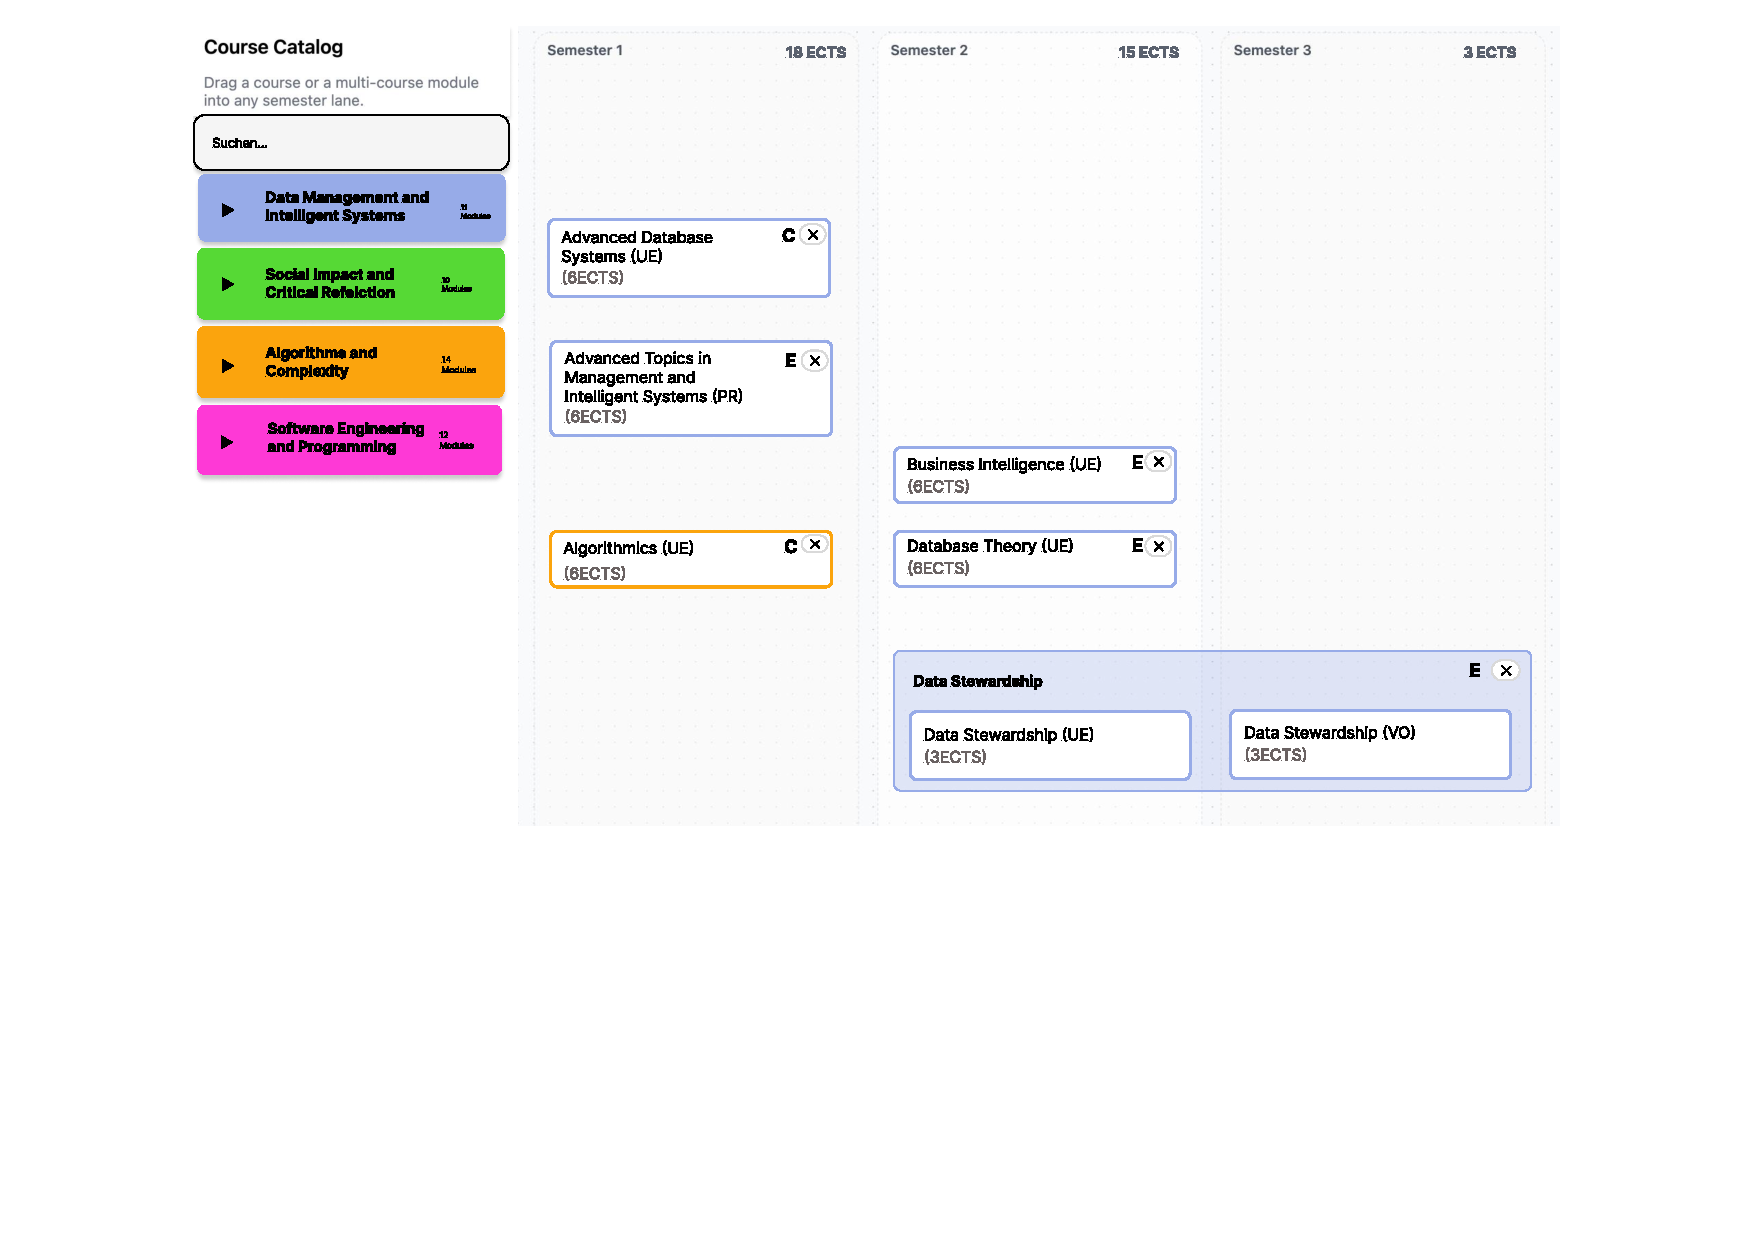
\includegraphics[width=\textwidth]{pictures/Prototype_TableView.pdf}
    \caption{Table View of the prototype: semester columns with running ECTS totals, a searchable catalogue sidebar, and courses and grouped modules placed as movable cards.}
    \label{fig:prototype-tableview}
\end{figure}

\begin{figure}[htbp]
    \centering
    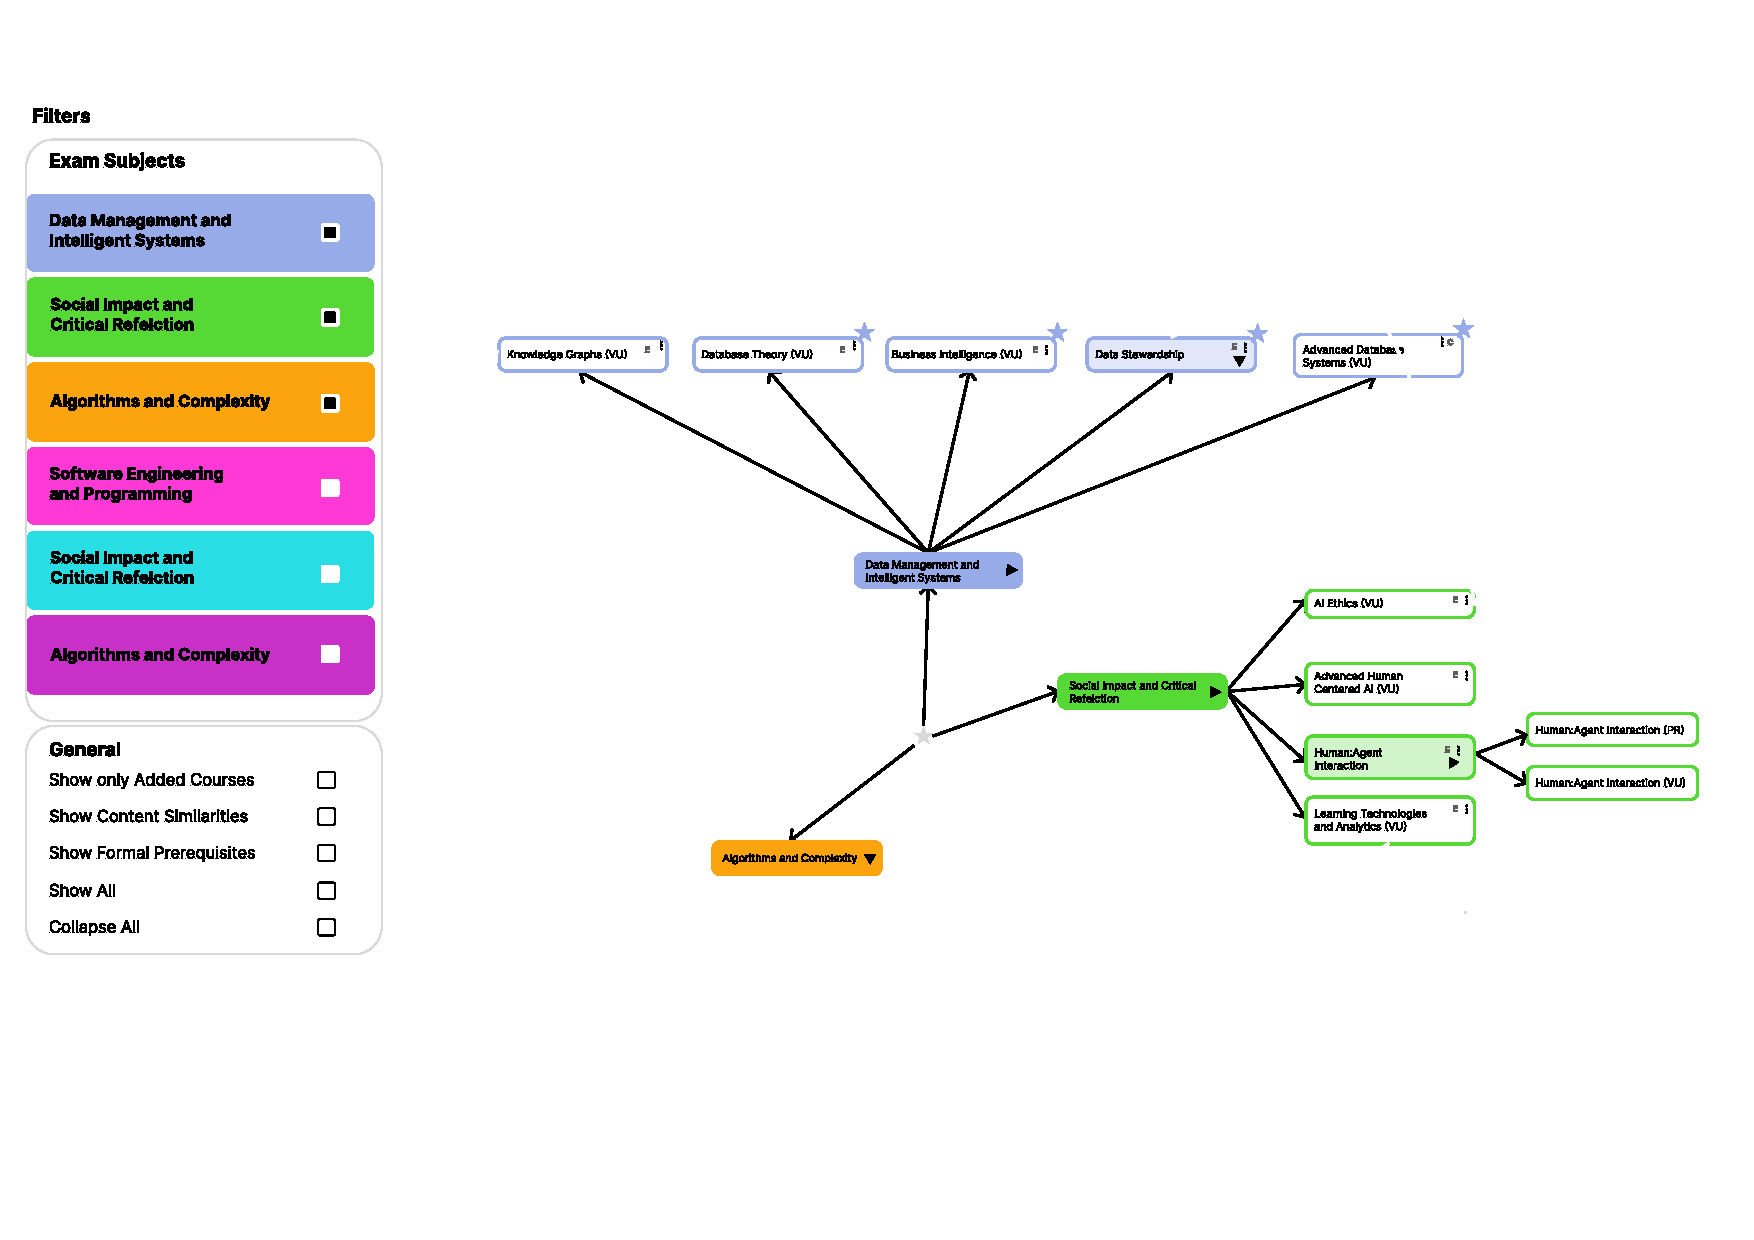
\includegraphics[width=\textwidth]{pictures/Prototype_GraphView.pdf}
    \caption{Graph View of the prototype: exam subjects, modules, and courses as colour-coded nodes, with filter controls, planned-course markers, and collapsible branches.}
    \label{fig:prototype-graphview}
\end{figure}

\begin{figure}[htbp]
    \centering
    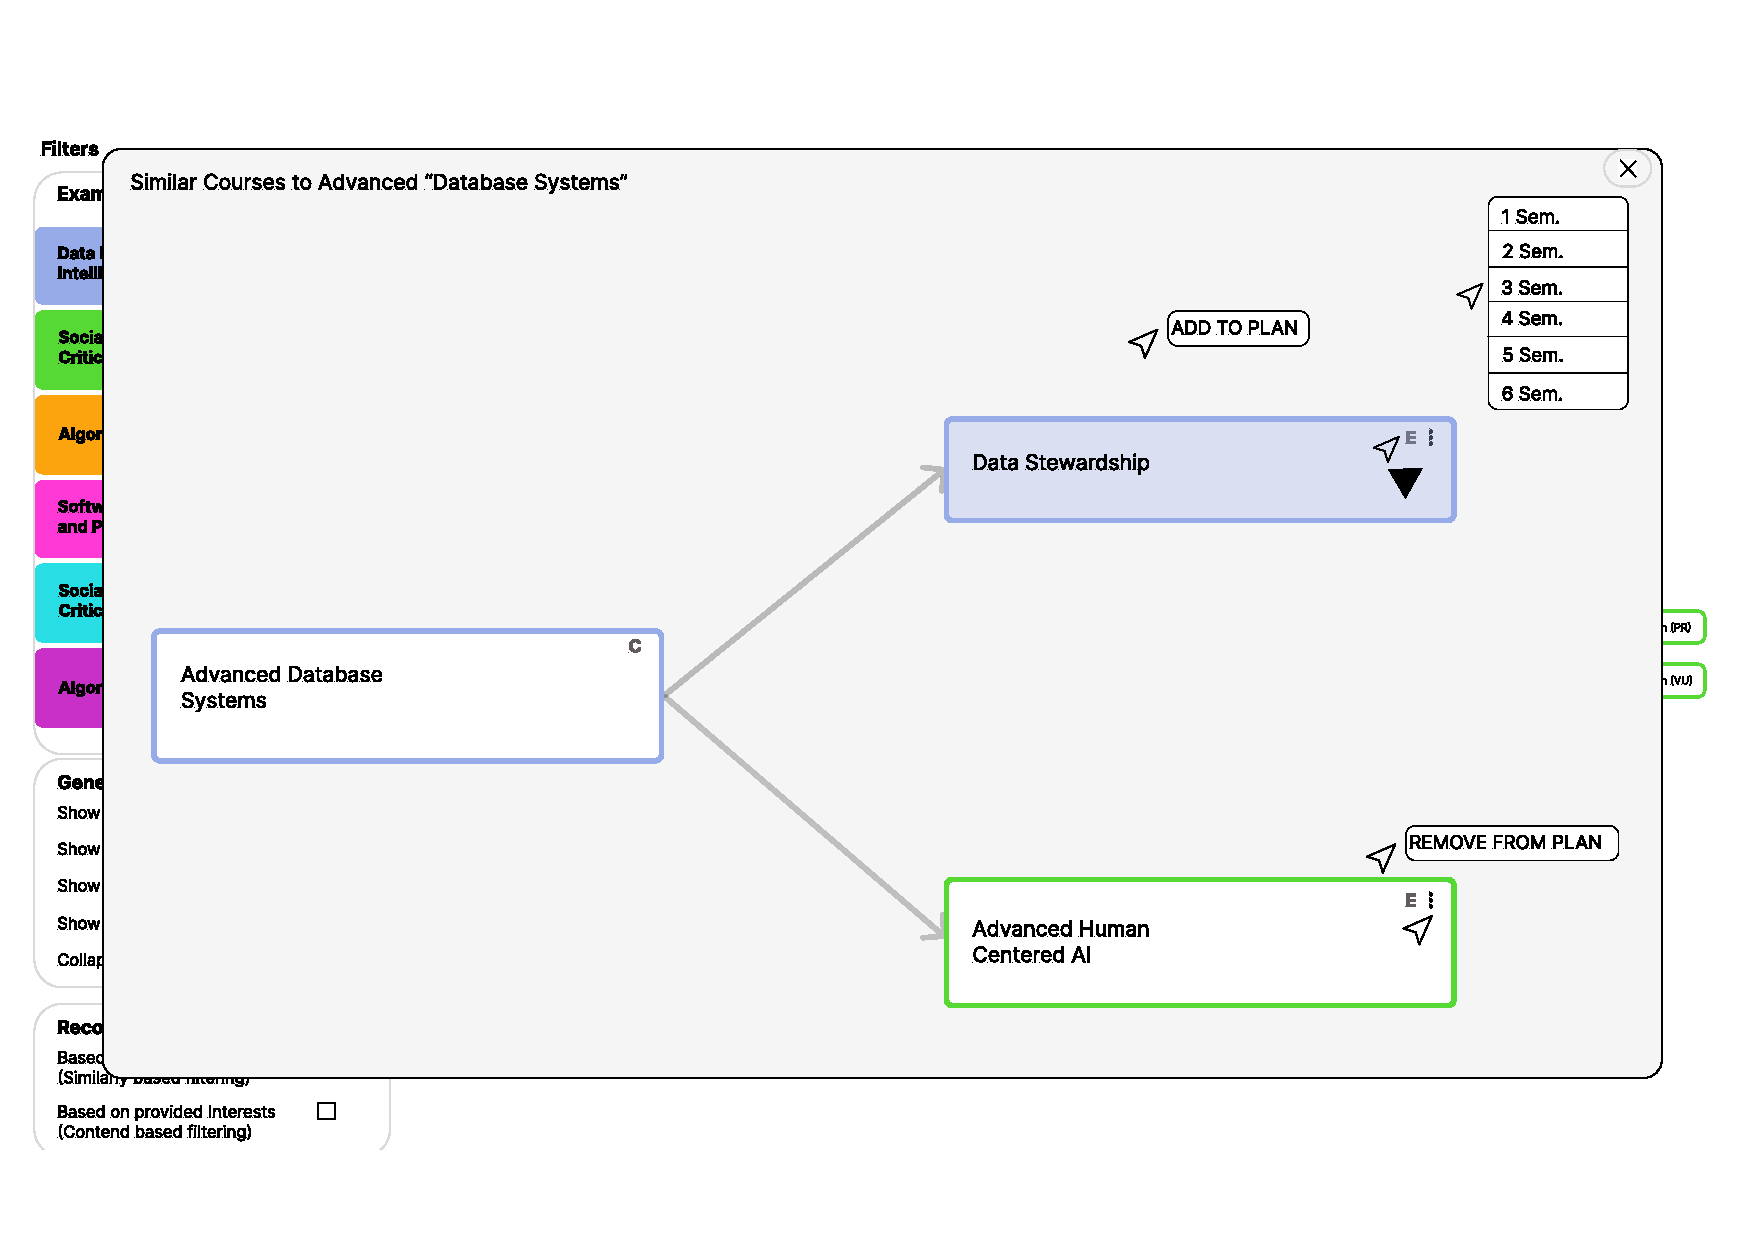
\includegraphics[width=\textwidth]{pictures/Prototype_SimilarCourses.pdf}
    \caption{Recommendation concept in the prototype: a focal course shown with related courses, add and remove actions, and a semester-selection control bridging into the plan.}
    \label{fig:prototype-recommendation}
\end{figure}

\paragraph{What the prototype did not represent.}
The prototype was visually detailed but not a functional system: it had no backend, no persistent data model, and no live rule-checking. Controls such as \enquote{Show Formal Prerequisites} and the recommendation actions were conceptual prompts for discussion, not validated computational features, and the recommendation views tested participants' expectations and acceptance conditions, not the quality of an actual algorithm. It also covered only a bounded subset of programmes and curriculum structures, so feedback about missing coverage was treated as a scope limitation of the elicitation artefact rather than a flaw in the interaction concept. In sum, the prototype functioned as a requirements-elicitation device for design and workflow discussion, not as a summative usability or system-performance evaluation instrument.

% ------------------------------------------------------------
\section{Participants and Recruitment}
\label{sec:participants-recruitment}

The formative study included six students from the Faculty of Informatics at TU~Wien: three Bachelor's students (Computer Science) and three Master's students (Software Engineering). The split was chosen to obtain perspectives at different degrees of curriculum familiarity and under different planning constraints, since a Bachelor's student working through broad foundational requirements and a Master's student choosing among specialised electives face different problems. Participants were eligible if they were enrolled in one of these two programmes, which is the population the tool is intended for.

With six participants from a single faculty, the aim was breadth of needs discovery rather than representativeness. The specification derived in Section~\ref{chap:from-themes-to-requirements} should accordingly be read as what this population needed, not as a statistically generalisable account of student planning.

\section{Procedure}
\label{sec:procedure}

Each session was a semi-structured interview combined with a think-aloud walkthrough of the prototype, run to a fixed plan of four phases: welcome and consent, current planning behaviour, prototype exploration, and reflection and wrap-up. Participants were asked for consent to audio recording before any questions, were told that the prototype was non-functional and that its gaps were the point of discussion, and were prompted to think aloud throughout the walkthrough. Sessions were conducted in German. The phase structure, the goal of each phase, and the full interview script with every prompt are given in Appendix~\ref{app:formative-interview-plan}.

\section{Analysis Method}
\label{sec:analysis-method}

The analysis follows the \emph{codebook} branch of thematic analysis (TA). Braun and Clarke describe TA as a family of related approaches rather than one method, differing in how they treat codes, themes, researcher subjectivity, and procedure~\cite[pp.~227--232]{braun_thematic_2022}, and distinguish three: \emph{coding-reliability} TA, \emph{codebook} TA, and \emph{reflexive} TA~\cite[pp.~235--236]{braun_thematic_2022}.

The choice among them follows from what this analysis has to produce. Its output is not an interpretation to be read on its own, but an intermediate object that has to carry forward into numbered requirements, so each theme must remain traceable to the excerpts behind it. That rules out reflexive TA, which develops themes as shared-meaning patterns arrived at through sustained interpretive engagement~\cite[pp.~35--36, 77--78]{braun_thematic_2022}: it was set aside on the shape of its output, not on the resources available for it. It also rules out coding-reliability TA, which treats researcher subjectivity mainly as a threat to accuracy and centres quality procedures such as multiple coders and inter-coder agreement~\cite[pp.~237--238]{braun_thematic_2022}. Braun and Clarke do not recommend such procedures for codebook TA, describing the approach instead as usable \enquote{by single researchers or teams}~\cite[pp.~236, 248]{braun_thematic_2022}. Codebook TA sits between the two, combining what Braun and Clarke call \enquote{Big Q} qualitative values, meaning a fully qualitative research paradigm, with a more structured approach to coding and early theme development~\cite[p.~242]{braun_thematic_2022}. That is the balance this study needs: enough structure to produce an auditable set of themes translatable into requirements, without the interpretive commitment of the one or the multi-coder apparatus of the other.

Codebook TA is described at the level of a cluster of approaches, and does not itself prescribe how a codebook is built and maintained across many transcripts. For that operational layer the analysis draws on framework analysis, which Braun and Clarke classify as a codebook approach~\cite[pp.~244--245]{braun_thematic_2022}. Framework analysis prescribes a structured charting procedure, in which the data are summarised by category into a matrix~\cite{gale_using_2013}, and it is that procedure the codebook construction here follows, together with established first-cycle coding practice, in which short labels are attached to individual excerpts.

The four steps below are presented in order for transparency, but the work moved repeatedly between coding, consolidation, review, and refinement. Writing about reflexive TA, Braun and Clarke frame their phases as \enquote{robust process guidelines, not rigid rules}~\cite[p.~10]{braun_thematic_2022} and the process as \enquote{progressive but recursive}~\cite[p.~36]{braun_thematic_2022}; the same holds here.

\paragraph{Data Preparation and Familiarisation.}
\label{sec:data-preparation}

All six interviews were audio-recorded, transcribed verbatim using Notta.ai\footnote{\url{https://www.notta.ai/}}, anonymised, and labelled I1--I6. The interviews were conducted in German; the excerpts quoted in this thesis are the author's translations, and the German originals are retained in the coding document alongside every code they informed. The transcripts were then read repeatedly, and passages expressing a practice, problem, information need, expectation, or evaluation relevant to study planning were marked as candidate excerpts.

Repeated reading of each transcript before any labelling corresponds to Braun and Clarke's familiarisation phase~\cite[pp.~42--49]{braun_thematic_2022}; marking the passages themselves already anticipates the coding phase, in which the analyst identifies segments that appear potentially relevant to the research question~\cite[p.~35]{braun_thematic_2022}.

\paragraph{Step 1 -- Initial Coding with Verbatim Evidence.}
\label{sec:initial-coding}

In the first formal coding phase, these excerpts were assigned short, inductively developed \gterm{code}{initial codes}. The purpose of this step was to stay close to participants' statements while beginning to capture analytically relevant aspects of practices, problems, information needs, expectations, and evaluations relevant to study planning, the same categories used to identify excerpts during familiarisation. In line with Braun and Clarke's description of coding, the codes were not treated merely as summaries of surface content, but as concise analytic labels for potentially relevant meanings in the data~\cite[pp.~51--71]{braun_thematic_2022}, following the first-cycle coding practice already introduced above.

Not every part of a transcript was coded this way: small talk, purely procedural exchanges, and content unrelated to study planning were left uncoded, while a single passage could inform more than one code where it carried more than one relevant meaning. A code's relevance to the final requirements comes from what it says, not from how much transcript text it covers or how many times it was mentioned.

Each code was stored together with at least one verbatim quote and the corresponding interview ID. This created an explicit analytic trail from interpretation back to source material and allowed later theme consolidation to remain grounded in the transcripts. Coding the six transcripts this way produced 435 initial codes (81, 75, 56, 88, 69 and 66 across I1--I6).

\paragraph{Example Code.}
\emph{Defining study planning as multi-level}
\begin{quote}
(I1) \enquote{…three levels… for my current semester, my deadlines and courses… then… next semester or the next few semesters. And then the third level… how am I on track for my entire degree, in percent or visually…}
\end{quote}

\paragraph{Step 2 -- Consolidation into a Codebook of Higher-Level Themes.}
\label{sec:theme-consolidation}

In the next step, conceptually similar initial codes were grouped into broader, higher-level themes. In the context of this thesis, these themes are design-relevant need categories: a stable label for a recurring, planning-related need, supported by the specific codes and verbatim excerpts that informed it. The purpose here was not to develop a rich thematic narrative about student identity or meaning-making, but to condense recurring planning-related needs into stable analytic categories that could later be translated into requirements.

Consolidation reduced these 435 initial codes to 64 themes, labelled T1--T64. To support this process, a codebook was maintained, recording for each theme a stable label and the collated verbatim excerpts that informed it, each tagged with the interview it came from.
This structured, traceable record-keeping is what the Framework Method's emphasis on transparent charting of data calls for (Section~\ref{sec:analysis-method})~\cite{gale_using_2013}.

Consolidation was iterative rather than a single grouping pass: definitions were revised where categories overlapped, previously coded segments were reconsidered, and candidate themes were adjusted until the codebook stabilised.

\paragraph{Step 3 -- Scope-Based Review and Refinement.}
\label{sec:scope-refinement}

Once the theme set had stabilised, it was reviewed against the five scope boundaries OOS1--OOS5 defined in the Methodology chapter (Section~\ref{sec:overall-scope}). Themes whose need lay outside them were removed from the carried-forward set.

This step corresponds to the review and refinement logic in thematic analysis: candidate themes must be checked against both the data and the research purpose, and they may be revised, collapsed, split, or discarded~\cite[pp.~35--36, 97--111]{braun_thematic_2022}. Braun and Clarke explicitly note that radical revision is common during this stage and that themes must be assessed in terms of both their internal coherence and their relevance to the research question~\cite[pp.~35--36]{braun_thematic_2022}. The review mattered here because the interviews also surfaced adjacent issues that were meaningful to participants but outside the intended design scope of the artefact. Two themes illustrate this. T26 asks for realistic workload estimates, meaning how much time a course takes other students in practice, beyond its ECTS figure; it was ruled out because such estimates would have to come from ratings or shared feedback by other students (OOS4). T38 asks for planning around the terms in which courses are offered; it was ruled out under OOS3, since the tool has no live link to the institutional systems that hold that information. Every exclusion is recorded against its theme in the codebook, naming the boundary or platform decision that excluded it.

\paragraph{Step 4 -- Post-Analytic Prioritisation for Implementation.}
\label{sec:prevalence-ranking}

Once the final theme set had been established, the themes were reviewed for their prevalence across participants, defined as the number of interviews in which a given theme occurred at least once. This step served implementation prioritisation for a first prototype iteration, not as evidence of a theme's analytic importance or as statistical generalisability. Braun and Clarke caution against treating frequency as the basis for thematic importance, noting that \enquote{whether a pattern helps us elucidate a key aspect of understanding our research topic is not determined by how many people said it}~\cite[p.~141]{braun_thematic_2022}. This caution is consistent with broader qualitative-methods guidance: Sandelowski warns against \enquote{acontextual counting}, where the frequency of a mention is taken as evidence of its importance~\cite[p.~239]{sandelowski_real_2001}.

\section{Findings}
\label{sec:formative-findings}

The analysis produced 435 initial codes across the six interviews, consolidated into 64 themes labelled T1--T64. The scope-based review of Step~3 carried 51 of these forward, ruled eleven out of scope, and set two aside as procedural artefacts of the interview situation itself. The complete codebook is reproduced in Appendix~\ref{app:codebook}: every theme with its label, the number of interviews it recurred in, which of those three outcomes it received, and all 436 excerpts that informed it, each in translation beside the German original.

Five themes recurred in all six interviews: course choice weighed against feasibility (T6), the unification of the institutional and personal tools students otherwise consult separately (T10), automatic checking of curriculum rules instead of manual tracking (T13), recommendations that are grounded and personally relevant instead of generic (T23), and the representation of prerequisites and their order (T31). Twelve further themes recurred in four or five of them; the count for every theme is given in the appendix table (Appendix~\ref{app:codebook}).

\paragraph{Output Artefacts and Traceability}
\label{sec:output-traceability}
The analysis produced one artefact this thesis carries: the consolidated theme codebook, reproduced in Appendix~\ref{app:codebook} with each theme's excerpts and the number of interviews it recurred in. It is this chapter's substantive result and the input Section~\ref{chap:from-themes-to-requirements} works from: each theme can be read against the evidence that produced it, and each feature derived there names the themes it rests on, so the chain runs in both directions.

% ------------------------------------------------------------
\section{From Themes to Requirements}
\label{chap:from-themes-to-requirements}

This section turns the themes above into features and testable requirements. It follows the logic of human-centred design, in which design rests on an explicit understanding of users, tasks and environments and proceeds through specifying the user requirements, producing design solutions, and evaluating them against those requirements~\cite{iso9241_210}, and that of requirements engineering, which identifies stakeholders and their needs and documents them in a form amenable to analysis, communication and subsequent implementation~\cite[p.~37]{nuseibeh_requirements_2000}.

Its outcome is the features-and-requirements specification that the Design and Implementation chapters build (Chapter~\ref{chap:design}, Chapter~\ref{chap:implementation}) and the evaluation reports against (Chapter~\ref{chap:evaluation}).

\subsection{Deriving Requirements from Themes}
\label{sec:derivation-process}

The starting point was the final theme set of Chapter~\ref{chap:formative-study}: 64 themes, each a design-relevant need category grounded in collated interview excerpts and linked throughout to that evidence, so that a requirement can be followed backwards to its qualitative origin.

Each theme was first read, together with the initial excerpts constituting it, to formulate a design implication, the guiding question being what the system must support if the need is to be addressed. Requirements were derived from themes rather than from individual utterances, since elicited material has to be interpreted before it can stand as a requirement~\cite[p.~39]{nuseibeh_requirements_2000}. Each theme yielded one or more candidate \gterm{requirement}{requirements}, written as statements of what the system must support rather than how it should be built. Related requirements were grouped into \emph{\gterm{feature}{features}}, a feature being one coherent capability of the product. Where several themes converged on one capability they shared a feature; where one theme implied different capabilities it fed more than one, so a requirement count is not tied one-to-one to its theme. Where something was deliberately left out of a feature, a short delineation records it, consistent with requirements-engineering practice, in which not all elicited needs are taken forward unchanged but must be bounded in a form manageable for development.

The chain this produces is \emph{interview evidence $\rightarrow$ code $\rightarrow$ theme $\rightarrow$ requirement $\rightarrow$ feature}, matching the derivation order above and the codebook Chapter~\ref{chap:formative-study} produced (Section~\ref{sec:output-traceability}). Linking a requirement back to what motivated it before any specification existed is what Gotel and Finkelstein call pre-requirements-specification traceability~\cite[p.~97]{gotel_analysis_1994}. Each feature accordingly names the themes it rests on by identifier, and each theme's excerpts are reproduced in Section~\ref{app:codebook}, so the chain can be followed in either direction.

\subsection{Resulting Features}
\label{sec:resulting-features}

The theme set yielded 13 features carrying 55 numbered requirements between them. The five scope boundaries OOS1 to OOS5 defined in the Methodology chapter (Section~\ref{sec:overall-scope}) apply throughout, and are referred to by those numbers here and in later chapters. Each feature carries a total importance score (Section~\ref{sec:prevalence-ranking}), the summed prevalence of its associated themes. Summing favours features that many themes converge on; the score was used once, to sequence implementation work, and no finding in Chapter~\ref{chap:evaluation} or Chapter~\ref{chap:discussion} depends on it. Table~\ref{tab:feature-summary} lists the result in descending order of that score, and Section~\ref{app:traceability-matrix} records, for each feature, the sections of Chapter~\ref{chap:design} that take it up. The full specifications are given in Section~\ref{app:feature-specs}, each in the same structure: title and identifier, importance score, associated themes, description and user evidence, derived requirements, and a delineation where one applies; they are cited from the Design chapter onward as, e.g., Feature~\ref{feat:004}, Req.~1.

The 13 features fall into three groups. Four are the planning core: getting curriculum data into the system without manual transcription (FEATURE-001), showing progress against the programme at three granularities (FEATURE-002), enforcing the curriculum's own rules (FEATURE-003), and moving a course from exploration in the graph to commitment in the table (FEATURE-004). Together they define the hybrid graph-table concept the rest of the thesis builds and tests. Four more add the judgement layer participants described around that core: semester feasibility (FEATURE-005), explainable recommendation (FEATURE-007), stage-appropriate onboarding (FEATURE-006), and replanning under disruption (FEATURE-008). The remaining five concern how the representation behaves once it is populated: density control (FEATURE-009), graph interpretability (FEATURE-010), visual and affective load (FEATURE-011), non-destructive recommendation display (FEATURE-012), and user-defined spatial grouping (FEATURE-013). The three groups run in descending score order, which is why implementation began with the first.

Two features contain requirements that were derived from the data but not carried into the implemented system, because of resource and time constraints during development: FEATURE-005, Req.~3 (self-assessed readiness profiles) and FEATURE-013, Reqs.~1, 3, and~4 (named, cross-view groups). Both are stated in the respective Delineation in Section~\ref{app:feature-specs} and are taken up as shortfalls in Chapter~\ref{chap:conclusion} (Section~\ref{sec:concl-rq-answers}). Every other exclusion recorded in a Delineation follows from a scope boundary, OOS2 to OOS4, or from a design decision stated there, not from what was built.

\begin{table}[htpb]
    \centering
    \footnotesize
    \begin{tabular}{@{}l>{\raggedright\arraybackslash}p{4.5cm}c>{\raggedright\arraybackslash}p{3.3cm}c@{}}
        \toprule
        \textbf{ID} & \textbf{Feature} & \textbf{Score} & \textbf{Associated themes} & \textbf{Reqs.} \\
        \midrule
        FEATURE-001 & Unified Data \& Tool Integration & 20 & T9, T10, T11, T12, T15, T37, T62 & 5 \\
        FEATURE-002 & Multi-Level Roadmap \& Progress \gterm{dashboard}{Dashboard} & 19 & T1, T16, T18, T19, T57 & 6 \\
        FEATURE-003 & Curriculum Rules \& Compliance Engine & 18 & T13, T17, T30, T31, T33, T63 & 5 \\
        FEATURE-004 & Graph-to-Table Planning Workflow & 15 & T20, T21, T44, T47, T61 & 6 \\
        FEATURE-005 & Feasibility Planning & 14 & T6, T35, T48, T49 & 3 \\
        FEATURE-007 & Evidence-Based, Explainable Recommendation Support & 13 & T23, T24, T45, T52 & 6 \\
        FEATURE-006 & Onboarding \& Guided Planning Transition & 12 & T5, T7, T59 & 2 \\
        FEATURE-008 & Constraint-Aware Replanning \& Disruption Handling & 9 & T4, T46, T56 & 4 \\
        FEATURE-009 & Overwhelm-Safe Browsing & 6 & T42, T50, T64 & 3 \\
        FEATURE-010 & Graph Interpretability & 5 & T27, T32, T40, T41 & 4 \\
        FEATURE-011 & Motivating Visual UI \& Emotional Load Reduction & 5 & T8, T54, T58 & 4 \\
        FEATURE-012 & Recommendation Presentation UX & 4 & T43, T55 & 3 \\
        FEATURE-013 & Spatial Organisation \& Grouping Controls & 3 & T28, T29 & 4 \\
        \bottomrule
    \end{tabular}
    \caption{The 13 features, in descending order of importance score, with the themes each was derived from and the number of requirements each carries. The full specifications are in Section~\ref{app:feature-specs}.}
    \label{tab:feature-summary}
\end{table}


\chapter{From Themes to Requirements}
\label{chap:from-themes-to-requirements}

This chapter turns the themes of Chapter~\ref{chap:formative-study} into features and testable requirements. It follows the logic of human-centred design, in which design rests on an explicit understanding of users, tasks and environments and proceeds through specifying the user requirements, producing design solutions, and evaluating them against those requirements~\cite{iso9241_210}, and that of requirements engineering, which identifies stakeholders and their needs and documents them in a form amenable to analysis, communication and subsequent implementation~\cite[p.~37]{nuseibeh_requirements_2000}.

Together with Chapter~\ref{chap:formative-study}, this chapter answers the first research question:

\begin{quote}
\textit{What are students' needs and resulting requirements for a hybrid graph-table interface that supports programme-level study planning and understanding of curriculum structure and course dependencies?}
\end{quote}

Its outcome is the features-and-requirements specification that the Design and Implementation chapters build (Chapter~\ref{chap:design}, Chapter~\ref{chap:implementation}) and the evaluation reports against (Chapter~\ref{chap:evaluation}).

\section{From Themes to Requirements}
\label{sec:derivation-process}

The starting point was the final theme set of Chapter~\ref{chap:formative-study}: 64 themes, each a design-relevant need category grounded in collated interview excerpts and linked throughout to that evidence, so that a requirement can be followed backwards to its qualitative origin.

Each theme was first read, together with the initial excerpts constituting it, to formulate a design implication, the guiding question being what the system must support if the need is to be addressed. Each theme, rather than a single utterance, is the operative expression of a stakeholder need: elicited material has to be interpreted, analysed and modelled before it can stand as a requirement~\cite[p.~39]{nuseibeh_requirements_2000}, and the theme is the unit at which that interpretation was recorded, with its excerpts behind it. Each theme then yielded one or more candidate \gterm{requirement}{requirements}, written as statements of what the system must support rather than how it should be built. Related requirements were grouped into \emph{\gterm{feature}{features}}, a feature being one coherent capability of the product. Where several themes converged on one capability they shared a feature; where one theme implied different capabilities it fed more than one, so a requirement count is not tied one-to-one to its theme. Where something was deliberately left out of a feature, a short delineation records it, consistent with requirements-engineering practice, in which not all elicited needs are taken forward unchanged but must be bounded in a form manageable for development.

The chain this produces is \emph{interview evidence $\rightarrow$ code $\rightarrow$ theme $\rightarrow$ requirement $\rightarrow$ feature}, matching the derivation order above and the codebook Chapter~\ref{chap:formative-study} produced (Section~\ref{sec:output-traceability}). Linking a requirement back to what motivated it before any specification existed is what Gotel and Finkelstein call pre-requirements-specification traceability~\cite[p.~96]{gotel_analysis_1994}. Each feature accordingly names the themes it rests on by identifier, and each theme's excerpts are reproduced in Section~\ref{app:codebook}, so the chain can be followed in either direction.

\section{Resulting Features}
\label{sec:resulting-features}

The theme set yielded 13 features carrying 55 numbered requirements between them. The five scope boundaries OOS1 to OOS5 defined in the Methodology chapter (Section~\ref{sec:overall-scope}) apply throughout, and are referred to by those numbers here and in later chapters. Each feature carries a total importance score (Section~\ref{sec:prevalence-ranking}), the summed prevalence of its associated themes, which was used to prioritise early implementation attention. Table~\ref{tab:feature-summary} lists the result in descending order of that score. The full specifications are given in Section~\ref{app:feature-specs}, each in the same structure: title and identifier, importance score, associated themes, description and user evidence, derived requirements, and a delineation where one applies; they are cited from the Design chapter onward as, e.g., Feature~\ref{feat:004}, Req.~1.

The score is a sum, not a mean, so it rewards breadth: a feature seven themes converge on outranks one that two themes raise more insistently. Normalising by theme count would order the specification differently. The order was used once, to sequence implementation work, and no finding in Chapter~\ref{chap:evaluation} or Chapter~\ref{chap:discussion} depends on it.

The 13 features fall into three groups. Four are the planning core: getting curriculum data into the system without manual transcription (FEATURE-001), showing progress against the programme at three granularities (FEATURE-002), enforcing the curriculum's own rules (FEATURE-003), and moving a course from exploration in the graph to commitment in the table (FEATURE-004). Together they define the hybrid graph--table concept the rest of the thesis builds and tests. Four more add the judgement layer participants described around that core: semester feasibility (FEATURE-005), explainable recommendation (FEATURE-007), stage-appropriate onboarding (FEATURE-006), and replanning under disruption (FEATURE-008). The remaining five concern how the representation behaves once it is populated: density control (FEATURE-009), graph interpretability (FEATURE-010), visual and affective load (FEATURE-011), non-destructive recommendation display (FEATURE-012), and user-defined spatial grouping (FEATURE-013). The three groups run in descending score order, which is why implementation began with the first.

Two features contain requirements that were derived from the data but not carried into the implemented system, because of resource and time constraints during development: FEATURE-005, Req.~3 (self-assessed readiness profiles) and FEATURE-013, Reqs.~1, 3, and~4 (named, cross-view groups). Both are stated in the respective Delineation in Section~\ref{app:feature-specs} and are taken up as shortfalls in Chapter~\ref{chap:discussion}. Every other exclusion recorded in a Delineation follows from a scope boundary, OOS2 to OOS4, or from a design decision stated there, not from what was built.

\begin{table}[htpb]
    \centering
    \footnotesize
    \begin{tabular}{@{}l>{\raggedright\arraybackslash}p{4.5cm}c>{\raggedright\arraybackslash}p{3.3cm}c@{}}
        \toprule
        \textbf{ID} & \textbf{Feature} & \textbf{Score} & \textbf{Associated themes} & \textbf{Reqs.} \\
        \midrule
        FEATURE-001 & Unified Data \& Tool Integration & 20 & T9, T10, T11, T12, T15, T37, T62 & 5 \\
        FEATURE-002 & Multi-Level Roadmap \& Progress \gterm{dashboard}{Dashboard} & 19 & T1, T16, T18, T19, T57 & 6 \\
        FEATURE-003 & Curriculum Rules \& Compliance Engine & 18 & T13, T17, T30, T31, T33, T63 & 5 \\
        FEATURE-004 & Graph-to-Table Planning Workflow & 15 & T20, T21, T44, T47, T61 & 6 \\
        FEATURE-005 & Feasibility Planning & 14 & T6, T35, T48, T49 & 3 \\
        FEATURE-007 & Evidence-Based, Explainable Recommendation Support & 13 & T23, T24, T45, T52 & 6 \\
        FEATURE-006 & Onboarding \& Guided Planning Transition & 12 & T5, T7, T59 & 2 \\
        FEATURE-008 & Constraint-Aware Replanning \& Disruption Handling & 9 & T4, T46, T56 & 4 \\
        FEATURE-009 & Overwhelm-Safe Browsing & 6 & T42, T50, T64 & 3 \\
        FEATURE-010 & Graph Interpretability & 5 & T27, T32, T40, T41 & 4 \\
        FEATURE-011 & Motivating Visual UI \& Emotional Load Reduction & 5 & T8, T54, T58 & 4 \\
        FEATURE-012 & Recommendation Presentation UX & 4 & T43, T55 & 3 \\
        FEATURE-013 & Spatial Organisation \& Grouping Controls & 3 & T28, T29 & 4 \\
        \bottomrule
    \end{tabular}
    \caption{The 13 features, in descending order of importance score, with the themes each was derived from and the number of requirements each carries. The full specifications are in Section~\ref{app:feature-specs}.}
    \label{tab:feature-summary}
\end{table}


\chapter{Design}
% ============================================================
%  Sections: General · Visual Design · Spatial Design
% ============================================================
\label{chap:design}
This chapter designs the tool from the specification of Chapter~\ref{chap:from-themes-to-requirements}. It moves from \emph{what} students need to \emph{how} the interface answers that need: each section states a decision, the requirement or evidence it answers, and the alternatives it was weighed against. It operates at level~3 of Munzner's nested model, visual encoding and interaction design~\cite{munzner2009}.

Together with Chapter~\ref{chap:implementation}, this chapter answers the second research question:

\begin{quote}
\textit{How can we design and implement a hybrid interface that combines graph-based visualisation with table-based planning to help students plan their studies and understand curriculum structure and course dependencies, based on those requirements?}
\end{quote}

The chapter is therefore organised by design dimension rather than by region of the screen: first the general architecture and the data model it rests on, then the visual encoding of curriculum elements, then interaction, and only then the individual views and features. This follows from the level Munzner's model places the chapter at, whose unit of design is the encoding or interaction technique, and which treats visual encoding and interaction as one level because the two are mutually interdependent~\cite[p.~922]{munzner2009}. An encoding such as the obligation channel, the subject-colour hierarchy or the course lifecycle is a property of the design, not of a panel: the same encoding appears in the Graph View, in the Table View and in the catalogue, and it has to be derived once from the evidence that motivates it rather than three times from wherever it happens to be visible. Organising by screen region would split each of those decisions across the regions that display it. The view- and feature-specific sections that follow the three dimension sections therefore describe only what is genuinely particular to a view or a feature, and refer back to the encodings rather than restating them.

The design decisions presented below are guided by the nine design principles for a study planning assistant in higher education established by Bartel et al.~\cite{bartel_design_2024}, alongside the direct empirical evidence gathered from the formative interviews.

Several decisions of the design originate directly from the Figma prototype used in the formative interviews (Chapter~\ref{chap:formative-study}). These elements were retained on the basis that six independent participant walkthroughs did not surface any objections to them. While this absence of objection provides indirect evidence that a concept is at least not actively unsuitable, it is acknowledged as weaker support than an explicit user requirement grounded in a stated need. Each assumption is discussed exactly where it applies in this chapter, clearly distinguishing between what was carried forward unchallenged and what was actively changed in response to feedback.

The tool's scope follows directly from Chapter~\ref{chap:methodology} and~\ref{chap:from-themes-to-requirements}, so all five OOS boundaries (Section~\ref{sec:overall-scope}) are already-settled inputs to design, not decisions this chapter makes or reconsiders. For each decision below, the rationale is stated explicitly exactly where the interface decision is discussed. These rationales are grounded in a feature or requirement, a prototype assumption not criticised during the formative interviews, common design knowledge, or specific published literature (such as Bartel et al.~\cite{bartel_design_2024} principles or Nielsen's usability heuristics~\cite{nielsen1994}). Where a genuine alternative was weighed during design, it is recorded alongside its rejection reason; not every decision below had a live alternative worth naming, so this is not claimed uniformly.

% ============================================================

\section{General Architecture and Data Model}
\label{sec:general}
This section establishes the frame every later section builds on, and moves from the outside inwards. It first divides the screen into panels, then settles what occupies the centre panel and why only one view may occupy it at a time. Its last two subsections leave the screen and describe the data model instead: the curriculum structure and the course obligation categories the interface is given to display. They are placed here because they are inputs to every visual encoding and every compliance rule in the later sections, which name their categories and cannot be derived without them.

% ------------------------------------------------------------
\subsection{Three-Panel Shell}
\label{sec:three-panels}
The outermost design decision is how the screen is divided, because that division fixes where every component described later in this chapter lives. Participants described planning as analogous to working at a physical desk (\enquote{like a desk… you just push things around} (T21)), which presupposes simultaneous access to multiple activities rather than sequential navigation between them. Feature~\ref{feat:004}, Req.~1 requires that the catalogue and the planning canvas be simultaneously visible, so a course can be added while observing the canvas update. Feature~\ref{feat:003}, Req.~1 requires compliance feedback to update in real time, ruling out placing it behind a tab where it would stop being ambient. Nielsen's recognition-rather-than-recall heuristic~\cite{nielsen1994} calls for minimising the user's memory load. A fixed region per function satisfies this directly: its position is stable, so a student recognises where a function lives instead of having to recall which mode a shared region currently holds.

Based on this evidence, the interface is divided into three spatially fixed, simultaneously visible panels (Figure~\ref{fig:three-panels}): a left panel offering three context-sensitive modes (Course Catalogue in Table View, filter controls in Graph View, and the independently-toggleable \gterm{recommendation-panel}{Recommendation Panel}), a centre panel hosting the active canvas (Table or Graph View), and a right panel hosting the Dashboard, which reports compliance and progress regardless of the active view. The sidebar-plus-canvas half of this structure is carried forward from the prototype unchanged; the two genuine additions are the right-panel Dashboard, which did not exist in the prototype (obligation was shown only as inline node indicators there) and was added in direct response to Feature~\ref{feat:003}, Req.~1, and the independent Recommendation Panel, in response to Feature~\ref{feat:012}, Req.~2.

A \emph{tab-based layout} was rejected because it makes the catalogue and the canvas mutually exclusive, which Feature~\ref{feat:004}, Req.~1 forbids, and a \emph{modal Dashboard} because compliance feedback surfaced only on request would let violations accumulate silently. The Recommendation Panel's placement is discussed in Section~\ref{sec:rec-panel}.

\begin{figure}[htbp]
\centering
\begin{tikzpicture}[font=\small, scale=0.88, transform shape]
  % Left panel (Widened to 2.8 to prevent text cutoff)
  \fill[panelgray, rounded corners=4pt] (0,0) rectangle (2.8,5.5);
  \draw[gray!50, rounded corners=4pt, line width=0.7pt] (0,0) rectangle (2.8,5.5);
  \node[font=\footnotesize\bfseries] at (1.4,5.15) {Left Panel};
  
  % Adjusted Y-coordinates down to prevent overlap with the heading
  \node[text width=2.6cm, align=center, font=\scriptsize] at (1.4,4.2)
    {Course Catalogue\\\textit{(Table View)}};
  \draw[gray!30, dashed, line width=0.5pt] (0.2,3.5) -- (2.6,3.5);
  
  \node[text width=2.6cm, align=center, font=\scriptsize] at (1.4,2.8)
    {Filter Controls\\\textit{(Graph View)}};
  \draw[gray!30, dashed, line width=0.5pt] (0.2,2.1) -- (2.6,2.1);
  
  % Forced line breaks to ensure 'Recommendation' fits nicely
  \node[text width=2.6cm, align=center, font=\scriptsize] at (1.4,1.3)
    {Recommendation\\Panel\\\textit{(independent toggle)}};

  % Centre panel (Adjusted start/end to accommodate wider side panels)
  \fill[white, rounded corners=4pt] (2.95,0) rectangle (8.05,5.5);
  \draw[gray!50, rounded corners=4pt, line width=0.7pt] (2.95,0) rectangle (8.05,5.5);
  \node[font=\footnotesize\bfseries] at (5.5,5.15) {Centre Panel};
  \node[text width=4.8cm, align=center, font=\scriptsize] at (5.5,4.3)
    {Table View \textit{or} Graph View\\(active canvas)};
  \fill[gray!15, rounded corners=3pt] (3.8,0.25) rectangle (7.2,0.75);
  \draw[gray!40, rounded corners=3pt, line width=0.5pt] (3.8,0.25) rectangle (7.2,0.75);
  \node[font=\scriptsize] at (5.5,0.5) {Table \quad $|$ \quad Graph};

  % Right panel (Shifted right to accommodate wider left panel)
  \fill[panelgray, rounded corners=4pt] (8.2,0) rectangle (11.0,5.5);
  \draw[gray!50, rounded corners=4pt, line width=0.7pt] (8.2,0) rectangle (11.0,5.5);
  \node[font=\footnotesize\bfseries] at (9.6,5.15) {Right Panel};
  \node[text width=2.6cm, align=center, font=\scriptsize] at (9.6,4.3)
    {Dashboard\\\textit{(compliance and progress)}};
\end{tikzpicture}
\caption{Three-panel shell. The left panel's catalogue and filter controls follow the active view, while the Recommendation Panel toggles independently. Centre: the active canvas. Right: the Dashboard.}
\label{fig:three-panels}
\end{figure}

\subsection{Graph and Table View: Mutually Exclusive Centre Panel}
\label{sec:mutual-exclusion}
Within that shell, the centre panel is where planning happens, and the next two subsections settle which view occupies it and what both are drawn on. Both views compete for the same resource, horizontal space, and for different reasons: the Graph View needs width to show the curriculum tree at legible node sizes, the Table View to give every semester a column wide enough for its course cards. At standard screen widths there is not enough of it for both at a usable scale. Participants themselves differentiated the two views by purpose: \enquote{graph used for exploration, not planning} (T20), which supports mutual exclusivity rather than permanent co-display.

Based on this, only one, Table View or Graph View, occupies the centre panel at any time. This division of labour, Graph View for exploration, Table View for commitment, was already present in the prototype (Chapter~\ref{chap:formative-study}) and was not questioned by any formative-study participant. The active view is toggled by a control in the toolbar.

A \emph{split-screen layout}, with the two views side by side, was rejected for the reason just given: neither retains usable width. A second alternative was a \emph{minimap or preview} of the inactive view. This was also rejected: a preview detailed enough to be informative would have required rendering a substantial second view, effectively reintroducing the space constraints of a split-screen layout. Conversely, a reduced preview that avoided these constraints provided too little information to justify its presence.

% ------------------------------------------------------------
\subsection{Unified Interactive Canvas for Both Views}
\label{sec:canvas}
Whichever of the two is active, it is drawn on the same surface. Spatial metaphors recurred when participants described planning: \enquote{like a desk… you just push things around} (T21), \enquote{I'd rather place them how I want} (T28). A static, column-sorted table cannot express spatial priority, distance-based de-emphasis, or personal groupings that participants explicitly requested (T28, T29). Feature~\ref{feat:013}, Req.~1 (free grouping) and Feature~\ref{feat:013}, Req.~2 (positions persist) require the canvas to hold arbitrary item positions. Direct manipulation replaces command syntax with action on the objects of interest themselves, kept visible and reversible~\cite{shneiderman1983}; dragging a course card into a semester is that action, where a form would be the syntax.

Based on this, both the Table View and the Graph View are rendered on an \emph{interactive, pannable, zoomable canvas}. Items (course, modules, table, graph structure) are positioned as absolute objects on the canvas. Users navigate by panning (scrolling the canvas in any direction) and zooming. Dragging items updates their position in real time. A configurable snap grid enforces positional alignment after a drag gesture for the Table View, producing ordered layouts without demanding fine motor precision. The visual representation of any item is identical in both views; sharing the same canvas model for both means the item definition is authored once (Feature~\ref{feat:004}, Req.~4: two-way synchronisation), eliminating the risk of visual inconsistency between views.

% ------------------------------------------------------------
\subsection{Curriculum Abstraction}
\label{sec:curriculum-abstraction}

Participants in the formative interviews described manual curriculum extraction from TISS, TU Wien's course and curriculum information system, as burdensome and error-prone: \enquote{clicking through TISS… pulling it out manually} (T37), \enquote{very error-prone… you might slip in the row} (T62). Relying on students to manually input and structure their own data violates Bartel et al.~\cite{bartel_design_2024} principle of \emph{centralisation of systems and information}, which argues against forcing students to cross-reference multiple decentralised sources like official PDFs. Furthermore, Feature~\ref{feat:003} requires curriculum compliance rules to operate on named, semantically meaningful categories (modules, exam subjects). Guided additionally by Bartel et al. principles of \emph{study-programme-specific personalisation} and the \emph{use of university identifiers}, the tool's data architecture ensures these categories are not generic; they must match the exact structural hierarchy of the specific study programme and utilise official university terminology.

Consequently, all curriculum data (programme structure, module composition, course list, ECTS values, obligation types, estimated weekly hours) is provided directly to the system. This imported data explicitly includes the official university abbreviations and course numbers, which are widespread among students and essential for fast, familiar information retrieval. 

To achieve this programme-specific tailoring without requiring manual setup, the imported curriculum is abstracted as a strict four-level hierarchy: 

Programme $\to$ Exam Subject $\to$ Module $\to$ \gterm{course}{Course Item}. 

This hierarchy is encoded as a fixed design constraint to perfectly match the institutional structure of the TU Wien programmes covered (Section~\ref{sec:overall-scope}; Figure~\ref{fig:curriculum-hierarchy}). A module containing exactly one Course Item is collapsed to that Course Item in the interface; an intermediate layer containing nothing but itself would add a hierarchy step without conveying information. OOS2 (Chapter~\ref{chap:methodology}) fixes the planning granularity at course-within-semester, which makes the Course Item the foundational level of this hierarchy.

Underpinning this user-facing data, every element of the hierarchy also carries a stable internal identifier that persists across data refreshes and across both views, ensuring that user selections remain stable (Feature~\ref{feat:001}, Req.~2). While the structural hierarchy and core curriculum data are strictly fixed, the system provides one minor exception: it allows students to manually override a course's term availability in their personal plan. This localised flexibility is necessary because actual course offerings change from year to year faster than a periodically-refreshed dataset can reliably track. 

Alternative data models were considered but rejected due to their inability to support automated compliance tracking. A \emph{flat course list} (with no structural hierarchy) was rejected because compliance rules explicitly reference modules and exam subjects as named, verifiable categories; a flat list fundamentally cannot represent these groupings. Similarly, a \emph{three-level hierarchy} (omitting the Exam Subject level) was rejected because the Compliance Engine must evaluate ECTS quotas at the exam-subject level, which represents a critical institutional constraint.


\subsection{Course Obligation Abstraction}
\label{sec:course-obligation-abstraction}

Driven by the same need for \emph{study-programme-specific personalisation}~\cite{bartel_design_2024} that motivated the structural hierarchy, the system must also accurately encode the rules governing which courses are required versus optional. To achieve this, the underlying abstraction was designed to accommodate the unique rules of both degree programmes defined in the tool's scope (Section~\ref{sec:overall-scope}) simultaneously, rather than being extracted from one programme and merely applied to the other. 

This unified approach is necessary because the two covered programmes define their obligation taxonomies differently. In the Bachelor programme, unmarked modules are \emph{Pflichtmodule} (mandatory); modules marked~(+) are \emph{Wahlmodule der engen Wahl} (quota-based narrow-choice electives); and modules marked~(*) are \emph{Wahlmodule der breiten Wahl} (broad-choice electives). In the Master programme, unmarked modules are likewise \emph{Pflichtmodule}, but modules marked~(+) are \emph{Core-Module}, acting as a gating condition rather than a separately countable requirement; modules marked~(*) are \emph{Wahlmodule}, selectable only once that core gate is satisfied. 

Because obligation types cannot be reduced to a single flat enumeration shared across both programmes, the underlying data model encodes these programme-specific semantics separately. However, to maintain a unified user experience, it exposes them uniformly at the interface level as a single three-tier encoding: \emph{mandatory / constrained elective / fully elective} (introduced in Section~\ref{sec:obligation}). For example, the Bachelor's quota-gated \emph{enge Wahl} and the Master's completion-gated \emph{Core} both surface as \emph{constrained electives}, since both impose a structural precondition beyond free choice. The abstraction was built to carry both programmes at once, and it does; how far it would carry beyond the two is untested here and is taken up in the Discussion (Chapter~\ref{chap:discussion}).

Furthermore, the system must handle alternative course formats without breaking these compliance and obligation rules. A small number of modules are officially offered in two structural formats: an integrated lecture-exercise course (VU) or a split lecture-plus-exercise pair (VO~+~UE). Both variants inherit the parent module's single obligation category. When a student selects one variant, the system automatically treats the alternative as satisfied, ensuring the module cannot be double-counted under two different course codes. The recommendation engine (Section~\ref{sec:rec-types-evidence}) is similarly designed to recognise these variant pairs, ensuring that a course already covered by an added variant is never redundantly recommended.

\begin{figure}[htbp]
\centering
\begin{tikzpicture}[
  box/.style={draw=gray!50, fill=gray!15, rounded corners=3pt, minimum width=2.0cm,
              minimum height=0.55cm, align=center, font=\scriptsize, inner sep=3pt},
  prog/.style={box},
  subj/.style={box},
  modul/.style={box},
  cours/.style={box},
  eg/.style={-{Stealth[length=4pt]}, gray!60, thin},
  dots/.style={font=\scriptsize, text=black}
]
  % 1st Level
  \node[prog]  (prog) at (0,-0.1)   {Programme};
  
  % 2nd Level
  \node[subj]  (sa)   at (3.5, 1.2) {Exam Subject A};
  \node[subj]  (sb)   at (3.5,-1.4) {Exam Subject B};
  
  % 3rd Level (Modules OR Collapsed Single Courses)
  \node[modul] (m1)   at (7.0, 2.0) {Module 1};
  \node[modul] (m2)   at (7.0, 0.4) {Module 2};
  
  \node[cours] (c5)   at (10.5,-1.0) {Course};
  \node[cours] (c6)   at (10.5,-1.8) {Course};
  
  % 4th Level (Standard Courses)
  \node[cours] (c1)   at (10.5, 2.4) {Course};
  \node[cours] (c2)   at (10.5, 1.6) {Course};
  \node[cours] (c3)   at (10.5, 0.8) {Course};
  \node[cours] (c4)   at (10.5, 0.0) {Course};
  
  % Edges from Programme
  \draw[eg] (prog.east) -- (sa.west);
  \draw[eg] (prog.east) -- (sb.west);
  
  % Edges from Exam Subjects
  \draw[eg] (sa.east)   -- (m1.west);
  \draw[eg] (sa.east)   -- (m2.west);
  \draw[eg] (sb.east)   -- (c5.west);
  \draw[eg] (sb.east)   -- (c6.west);
  
  % Edges from Modules to Courses
  \draw[eg] (m1.east)   -- (c1.west);
  \draw[eg] (m1.east)   -- (c2.west);
  \draw[eg] (m2.east)   -- (c3.west);
  \draw[eg] (m2.east)   -- (c4.west);
  
  % Column Labels
  \node[font=\tiny] at (0,-2.95)    {Programme};
  \node[font=\tiny] at (3.5,-2.95)  {Exam Subject};
  \node[font=\tiny] at (7.0,-2.95)  {Module};
  \node[font=\tiny] at (10.5,-2.95) {Course};

  % The two single-course modules: the module node is not drawn, so the edge
  % from the exam subject crosses the module column to reach the course.
\end{tikzpicture}
\caption{Four-level curriculum hierarchy. Modules holding several courses keep their intermediate node; a module holding exactly one course is not drawn, and its course attaches directly to the exam subject.}
\label{fig:curriculum-hierarchy}
\end{figure}

\section{Visual Design of Curriculum Elements}
\label{sec:visual}
A recurring theme of the formative interviews was a preference for icon- and colour-based communication over text, T54 reporting that \enquote{too much text is off-putting}. Feature~\ref{feat:011}, Req.~1 records this as the requirement for a \emph{visual-first, low-text} interface, and the encodings below are how the design meets it: each carries on a visual channel what a card would otherwise have to spell out, with text kept as a redundant confirmation.

% ------------------------------------------------------------

\subsection{Course Obligation Encoding}
\label{sec:obligation}

Obligation type was named as a primary filter dimension: \enquote{mandatory… narrow elective… broad elective} (T42). Obligation type must be readable on every card without opening any popover, because it is the most common criterion for deciding whether to explore a course further.

Based on Section~\ref{sec:course-obligation-abstraction}, a course or a module can have three obligation types: mandatory, constrained elective, fully elective (Figure~\ref{fig:obligation-rings}). This is encoded in border weight, an ordered channel of three steps: a thick border denotes mandatory, a medium border constrained elective, and a thin border fully elective. A short text label naming the obligation category is additionally shown in the card footer, again as a secondary, redundant confirmation rather than the primary channel.

Border thickness as the primary channel is also a change from the prototype (Section~\ref{sec:prototype-elicitation}), not a carried-forward assumption: the prototype's obligation indicator was a visible letter badge (M/C/E) directly on each node, with border thickness introduced here instead and a text label introduced as the secondary confirmation just described. This shift is not traceable to a specific interview statement about obligation encoding itself, but it is a direct application of the visual-first, low-text principle (T54, Feature~\ref{feat:011}, Req.~1): a border-weight difference is read pre-attentively, while a letter requires serial reading.

A \emph{multiple concentric border rings} treatment (e.g.\ one ring for elective, two for constrained, three for mandatory, rather than one border of varying thickness) was considered and rejected: adding rings either grows the card outward, which conflicts with the fixed card geometry the snap-grid and table layout depend on, or grows inward at the expense of interior content space, and beyond two rings the count becomes hard to distinguish at a glance at typical card sizes. A single border of varying thickness avoids both problems.
\begin{figure}[htbp]
\centering
\begin{tikzpicture}[font=\scriptsize, scale=0.85, transform shape]
  \def\cw{2.4}\def\ch{2.8}\def\rc{subjectblue}

  % Broad Elective — thin ring
  \fill[white, rounded corners=3pt] (0,0) rectangle (\cw,\ch);
  \draw[\rc, line width=1.0pt, rounded corners=3pt] (0,0) rectangle (\cw,\ch);
  \node[font=\scriptsize\bfseries,text width=2.8cm,align=center] at (1.2,-0.4) {Fully Elective};
  \node[font=\tiny] at (1.2,-0.95) {thin border};

  % Core/Narrow Elective — medium ring
  \def\ox{3.6}
  \fill[white, rounded corners=3pt] (\ox,0) rectangle (\ox+\cw,\ch);
  \draw[\rc, line width=2.0pt, rounded corners=3pt] (\ox,0) rectangle (\ox+\cw,\ch);
  \node[font=\scriptsize\bfseries,text width=2.8cm,align=center] at (\ox+1.2,-0.4) {Constrained Elective};
  \node[font=\tiny] at (\ox+1.2,-0.95) {medium border};

  % Mandatory — thick ring
  \def\ox{7.2}
  \fill[white, rounded corners=3pt] (\ox,0) rectangle (\ox+\cw,\ch);
  \draw[\rc, line width=3.0pt, rounded corners=3pt] (\ox,0) rectangle (\ox+\cw,\ch);
  \node[font=\scriptsize\bfseries,text width=2.8cm,align=center] at (\ox+1.2,-0.4) {Mandatory};
  \node[font=\tiny] at (\ox+1.2,-0.95) {thick border};

\end{tikzpicture}
\caption{Obligation type encoding using three levels of border thickness. Border weight distinguishes obligation categories without using hue, thereby avoiding interference with the subject colour channel.}
\label{fig:obligation-rings}
\end{figure}


% ------------------------------------------------------------
\subsection{Planning Status Encoding}
\label{sec:status}

Feature~\ref{feat:002}, Req.~4 requires that the system distinguishes not-planned, planned, and completed states using consistent visual encodings across both views. Participants requested visual differentiation of states: \enquote{greyed out} and \enquote{star means finished} (T19), and \enquote{colour-based marking for rapid recognition} (T19). Feature~\ref{feat:011}, Req.~2 specifies that completed items should be faded while preserving an accessible record.

To achieve this, each module and course card encodes its \gterm{planning-status}{planning status} using two pre-attentive visual channels: fill lightness and border saturation. Hue is explicitly avoided here because it is reserved for the subject-colour hierarchy (Section~\ref{sec:subject-colour}). Since lightness and saturation are perceptually separable from hue, both encoding systems can coexist without visual interference. The system distinguishes four distinct states:

\begin{itemize}
  \item Not planned: white fill, full-saturation subject-colour border.
  \item Parked: white fill, full-saturation subject-colour border, identical to not-planned; the parked state is distinguished by a text label on the card (Figure~\ref{fig:status-encoding}).
  \item Planned: light grey fill, full-saturation subject-colour border.
  \item Done: reduced opacity overall, border desaturated to neutral grey; the card \enquote{recedes} visually.
\end{itemize}
The states are also illustrated in Figure~\ref{fig:status-encoding}. To prevent confusion, a short text label (e.g., \enquote{planned}, \enquote{done}) in the card footer acts as a redundant confirmation of the visual state. Because lightness and saturation are subtler than colour changes, relying on them alone could cause students to miss their planning status. Adding this small text label ensures clarity while still honouring the visual-first, low-text design required by Feature~\ref{feat:011}, Req.~1 (T54).

\emph{Icon-only status} was rejected because icons are already reserved for actions on cards (Section~\ref{sec:action-buttons}), and using one visual element both to show state and to change it would blur representation and interaction.

\begin{figure}[htbp]
\centering
\begin{tikzpicture}[font=\scriptsize, scale=0.85, transform shape]
  \def\cw{2.0}\def\ch{2.8}
  % Card 1: Not Planned
  \fill[white, rounded corners=3pt] (0,0) rectangle (\cw,\ch);
  \draw[subjectblue, line width=2pt, rounded corners=3pt] (0,0) rectangle (\cw,\ch);
  \node[text=black,font=\tiny,text width=1.8cm,align=center] at (1.0,1.8) {Course Name};
  \node[text=black,font=\tiny] at (1.0,1.2) {4.5~ECTS};
  \node[font=\scriptsize\bfseries] at (1.0,-0.4) {Not Planned};
  \node[font=\tiny,text width=2.1cm,align=center] at (1.0,-1.0) 
  {white fill, coloured border};
    % Card 2: Parked
    \def\ox{2.5}
    \fill[white, rounded corners=3pt] (\ox,0) rectangle (\ox+\cw,\ch);
    \draw[subjectblue, line width=2pt, rounded corners=3pt] (\ox,0) rectangle (\ox+\cw,\ch);
    \fill[subjectblue!15, rounded corners=2pt] (\ox+0.1,\ch-0.5) rectangle (\ox+0.9,\ch-0.15);
    \node[font=\tiny, text=subjectblue] at (\ox+0.5,\ch-0.32) {Parked};
    \node[text=black,font=\tiny,text width=1.8cm,align=center] at (\ox+1.0,1.55) {Course Name};
    \node[text=black,font=\tiny] at (\ox+1.0,1.0) {4.5~ECTS};
    \node[font=\scriptsize\bfseries] at (\ox+1.0,-0.4) {Parked};
    \node[font=\tiny,text width=2.1cm,align=center] at (\ox+1.0,-1.0)
    {white fill, label badge};
    % Card 3: Planned
    \def\ox{5.0}
    \fill[plannedfill, rounded corners=3pt] (\ox,0) rectangle (\ox+\cw,\ch);
    \draw[subjectblue, line width=2pt, rounded corners=3pt] (\ox,0) rectangle (\ox+\cw,\ch);
    \node[text=black,font=\tiny,text width=1.8cm,align=center] at (\ox+1.0,1.8) {Course Name};
    \node[text=black,font=\tiny] at (\ox+1.0,1.2) {4.5~ECTS};
    \node[font=\scriptsize\bfseries] at (\ox+1.0,-0.4) {Planned};
    \node[font=\tiny,text width=2.1cm,align=center] at (\ox+1.0,-1.0)
    {grey fill, coloured border};
  % Card 4: Done -- explicitly light colours rather than a subtle opacity scope, so the fade is actually visible on the page
  \def\ox{7.5}
  \fill[donefill, rounded corners=3pt] (\ox,0) rectangle (\ox+\cw,\ch);
  % Same 2pt weight as the other three: border thickness is the obligation channel
  % (Section obligation), and must not read as a status difference here.
  \draw[doneborder, line width=2pt, rounded corners=3pt] (\ox,0) rectangle (\ox+\cw,\ch);
  \node[text=gray!70,font=\tiny,text width=1.8cm,align=center] at (\ox+1.0,1.8) {Course Name};
  \node[text=gray!70,font=\tiny] at (\ox+1.0,1.2) {4.5~ECTS};
  \node[font=\scriptsize\bfseries,text=gray!70] at (\ox+1.0,-0.4) {Done};
  \node[font=\tiny,text width=2.1cm,align=center] at (\ox+1.0,-1.0) {light grey fill, light grey border and text};
\end{tikzpicture}
\caption{Four-state planning status encoding. Status is communicated through fill lightness and border saturation.}
\label{fig:status-encoding}
\end{figure}

% ------------------------------------------------------------
\subsection{Subject Colour Hierarchy}
\label{sec:subject-colour}
The three-level colour hierarchy emerged during iterative prototyping and was retained throughout the interview phase; participants did not question the use of subject-level colour as the primary grouping cue. Furthermore, Feature~\ref{feat:011}, Req.~1 requires colour semantics to remain stable across views.

To achieve this, each exam subject is represented by a unique, perceptually distinct hue. Hues are assigned deterministically based on the subject name and spread across the hue wheel with a minimum separation to keep adjacent subjects distinguishable. The red range is explicitly excluded from this assignable pool, because red is strictly reserved elsewhere in the interface for compliance-violation and incomplete-status signalling (Section~\ref{sec:compliance}); allowing a subject to randomly receive a red hue would risk it visually reading as a warning.

The assigned hue is then propagated consistently across the visual hierarchy using three levels of intensity. This approach is grounded in the perceptual principle of \emph{common region}~\cite{palmer1992}: elements inside one bounded area, whether bounded by a shared tint or by a border, group together strongly enough to override proximity and similarity, which reduces the need for text labels (Feature~\ref{feat:011}, Req.~1; T54).
\begin{enumerate}
  \item \textbf{Exam subject:} full background saturation and highest visual prominence, serving as the spatial anchor for the subject area.
  \item \textbf{Module:} the same hue applied as a low-intensity background tint (approximately 20\,\% opacity). This wash supports rapid visual grouping at the module level while keeping visual interference low. 
  \item \textbf{Course:} the full primary hue applied exclusively to the card border. This allows subject membership to remain clearly visible on each card (even when filtered or densely packed) while leaving the card interior available for status encoding. 
\end{enumerate}

Alternative encodings were considered but rejected. \emph{Full-saturation} subject colour on all cards was rejected because large coloured surfaces increase visual load, reduce text contrast, and flatten the intended hierarchy. \emph{Label-only subject encoding} was rejected because it forces serial reading instead of enabling immediate, pre-attentive grouping. \emph{Module-level hue assignment} was rejected because the high number of modules would exceed the set of reliably distinguishable hues, destroying cross-module coherence within a subject area. Figure~\ref{fig:colour-intensity} illustrates the final colour hierarchy.
\begin{figure}[htbp]
\centering
\begin{tikzpicture}[font=\small, scale=0.88, transform shape]
  % --- Level 1: Exam Subject Header (full saturation) ---
  \fill[subjectblue, rounded corners=4pt] (0,4.4) rectangle (3.6,5.2);
  \node[text=white, font=\footnotesize\bfseries] at (1.8,4.8) {Exam Subject A};

  % --- Level 2: Module (separate tinted element) ---
  \fill[subjectblue20, rounded corners=3pt] (0,2.8) rectangle (3.6,3.8);
  \draw[subjectblue, line width=1.0pt, rounded corners=3pt]
    (0,2.8) rectangle (3.6,3.8);
  \node[font=\scriptsize] at (1.8,3.3) {Module A};

  % --- Level 3: Course Card (separate white card with coloured border) ---
  \fill[white, rounded corners=2pt] (0,1.0) rectangle (3.6,2.2);
  \draw[subjectblue, line width=1.8pt, rounded corners=2pt]
    (0,1.0) rectangle (3.6,2.2);
  \node[font=\scriptsize] at (1.8,1.6) {Course Card};

  % Annotation arrows + labels on the right
  \draw[-{Stealth[length=4pt]}, gray!60] (3.7,4.8) -- (5.0,4.8);
  \draw[-{Stealth[length=4pt]}, gray!60] (3.7,3.3) -- (5.0,3.3);
  \draw[-{Stealth[length=4pt]}, gray!60] (3.7,1.6) -- (5.0,1.6);

  \node[right, font=\scriptsize, text width=4.5cm] at (5.05,4.8)
    {\emph{Full saturation}\\ Subject header node};

  \node[right, font=\scriptsize, text width=4.5cm] at (5.05,3.3)
    {\emph{Opacity wash + border}\\ Module element};

  \node[right, font=\scriptsize, text width=4.5cm] at (5.05,1.6)
    {\emph{Full-saturation border}\\ Course card outline};

  % Intensity arrow on the left
  \draw[-{Stealth[length=5pt]}, gray!50, line width=0.8pt]
    (-0.8,0.8) -- (-0.8,5.4);
  \node[rotate=90, font=\scriptsize] at (-1.2,3.1)
    {Increasing intensity $\longrightarrow$};
\end{tikzpicture}
\caption{Subject colour intensity hierarchy. One exam-subject hue applied at three levels: full saturation in the header, a 20\,\% tint on the module, and a full-saturation course-card border.}
\label{fig:colour-intensity}
\end{figure}
% ------------------------------------------------------------
\subsection{Text Content Across Hierarchy Levels}
\label{sec:text-content}
Overly dense text was reported as off-putting (T54). To support an always-current and legible planning view, students requested that key attributes like ECTS, \gterm{obligation-category}{obligation type}, and completion status remain visible at a glance (T16). Furthermore, they explicitly requested that module completion status be visible directly on the canvas, rather than restricted solely to the Dashboard (T57; Feature~\ref{feat:002}, Req.~3). 

To achieve this, the design minimises text and adapts it to the informational role of each hierarchy level. Wienand et al.~\cite{wienand_design_2024}, designing an e-learning platform for a different domain, report that a complicated navigation structure was a source of student frustration in the system they replaced, and chunk their own content so that each unit is displayed as a tile, giving what they call an \enquote{index card-like presentation}. The parallel is with the chunking rather than with the domain: this interface adopts a similarly card-based layout to avoid dense text (T54), so the text within each unit is strictly constrained, and each level carries only what a decision at that level needs (Figure~\ref{fig:card-text}).

An exam-subject card is read for orientation, so it carries the subject name and the extent of what it contains, and nothing further. A module header is read to answer one question, whether the module's quota is met, so it aggregates: name, total ECTS, obligation type and a status indicator. A course card is where an actual placement decision is made, and it is divided into three fixed zones. Its header carries the short course-code abbreviation, the course-type indicator and the term the course is offered in, applying Bartel et al.~\cite{bartel_design_2024} principle of relying on recognised university identifiers rather than inventing interface shorthand. Its title is the primary identifier and is clamped to two lines, which keeps card heights uniform for the snap-grid alignment system and keeps dense plans scannable. Its footer carries the three most frequently needed attributes: ECTS value, obligation type and status.

\begin{figure}[htbp]
\centering
\begin{tikzpicture}[font=\scriptsize,
  ann/.style={font=\tiny, text=black, anchor=west, text width=4.6cm, align=left},
  tick/.style={gray!55, thin}]

  % --- Exam subject card ---
  \draw[gray!60, line width=0.8pt, rounded corners=3pt, fill=white] (0,0) rectangle (4.4,1.0);
  \node[font=\scriptsize\bfseries] at (2.2,0.68) {Exam Subject A};
  \node[font=\tiny] at (2.2,0.3) {6 modules \textperiodcentered\ 14 courses};
  \draw[tick] (4.4,0.5) -- (5.0,0.5);
  \node[ann] at (5.05,0.5) {read for orientation: the name and how much it contains};

  % --- Module header ---
  \draw[gray!60, line width=0.8pt, rounded corners=3pt, fill=white] (0,-1.5) rectangle (4.4,-0.5);
  \node[font=\scriptsize\bfseries, anchor=west] at (0.18,-0.82) {Module A1};
  \node[font=\tiny, anchor=east] at (4.22,-0.82) {12~ECTS};
  \node[font=\tiny, anchor=west] at (0.18,-1.2) {Mandatory \textperiodcentered\ 2 of 4 done};
  \draw[tick] (4.4,-1.0) -- (5.0,-1.0);
  \node[ann] at (5.05,-1.0) {read for one question, whether the quota is met: aggregated progress};

  % --- Course card, three fixed zones ---
  \draw[gray!60, line width=0.8pt, rounded corners=3pt, fill=white] (0,-4.5) rectangle (4.4,-2.0);
  \draw[tick] (0,-2.55) -- (4.4,-2.55);
  \draw[tick] (0,-4.05) -- (4.4,-4.05);
  \node[font=\tiny] at (2.2,-2.28) {NS \ $|$ \ VU \ $|$ \ winter};
  \node[font=\scriptsize\bfseries, text width=3.9cm, align=center] at (2.2,-3.3) {Network Security};
  \node[font=\tiny] at (2.2,-4.28) {6~ECTS \textperiodcentered\ Mandatory \textperiodcentered\ planned};

  \draw[tick] (4.4,-2.28) -- (5.0,-2.28);
  \node[ann] at (5.05,-2.28) {header: official abbreviation, course type, term};
  \draw[tick] (4.4,-3.3) -- (5.0,-3.3);
  \node[ann] at (5.05,-3.3) {title: the primary identifier, clamped to two lines so card heights stay uniform};
  \draw[tick] (4.4,-4.28) -- (5.0,-4.28);
  \node[ann] at (5.05,-4.28) {footer: the three attributes needed most often};
\end{tikzpicture}
\caption{Text carried at each hierarchy level. The exam-subject card states only extent, the module header aggregates progress, and the course card divides its text into three zones of fixed height.}
\label{fig:card-text}
\end{figure}


Three alternatives were weighed and rejected, each on the same trade between information and height: \emph{richer metadata on course cards} roughly doubles card height for information a routine placement does not need (T54); \emph{module headers reduced to name and ECTS} force an expand or a Dashboard visit to read progress; and \emph{a full course list in the module header} makes a collapsed module nearly as tall as an expanded one. 
% ------------------------------------------------------------

\section{Interaction Design}
\label{sec:interaction}
The subsections below proceed from the overall workflow a student follows, to the underlying state model that workflow operates on, to the general interaction principles (dual drag/button paths, context-sensitive actions) applied throughout, to the specific mechanisms (Semester Picker, popover, module interaction) built from those principles. Because these principles hold across both views, they are stated before the views themselves. Two surfaces they act on are therefore named here and designed later: a \emph{semester lane}, the column holding the courses assigned to one semester, and the \gterm{parking-stage}{Parking Stage}, the area beside those lanes holding courses saved but not yet assigned to a term (both Section~\ref{sec:table-view}).


\subsection{Planning Workflow}
\label{sec:workflow}

Students build their curricula in an exploration-first sequence. As one participant noted, finding interesting courses is \enquote{cool as a first step… not thinking yet about which semester} (T20). Students distinctly separate the act of exploring options from the act of committing them to a timeline, explicitly stating that the \enquote{graph used for exploration, not planning} (T20). 

To support this mental model and provide a guided onboarding experience (Feature~\ref{feat:006}, Req.~1), the interface introduces an intermediate staging area between discovery and semester assignment (Feature~\ref{feat:004}, Req.~2). Consequently, the tool is designed around a three-stage planning workflow (Figure~\ref{fig:workflow}):
\begin{enumerate}
  \item \textbf{Browse:} The student opens the Graph View or the Sidebar and explores the full curriculum using search, filters, and collapse controls to manage visual density.
  \item \textbf{Shortlist:} The student parks interesting courses into the Parking Stage without needing to commit them to a specific semester.
  \item \textbf{Assign:} The student switches to the Table View and drags parked courses into semester lanes, or uses the Semester Picker to assign them directly.
\end{enumerate}

This intended sequence is gently surfaced through the onboarding tooltip flow and the default-collapsed graph state, which encourages high-level exploration before commitment. Furthermore, the Parking Stage is positioned prominently at the top of every Semester Picker (Section~\ref{sec:semester-picker}) to bridge the gap between shortlisting and assigning. 

The workflow does not force staging for every decision. A student who already knows their plan can bypass the Shortlist step entirely, assigning a course directly to a semester using the context-sensitive Semester Picker (Section~\ref{sec:semester-picker}), as illustrated by the direct assignment path in Figure~\ref{fig:workflow}.

\begin{figure}[htbp]
\centering
\begin{tikzpicture}[font=\small, scale=0.88, transform shape]
  \def\bw{3.4}\def\bh{3.0}

  % Step 1: Browse
  \fill[subjectblue20, rounded corners=5pt] (0,0) rectangle (\bw,\bh);
  \draw[subjectblue!50, line width=0.8pt, rounded corners=5pt]
    (0,0) rectangle (\bw,\bh);
  \node[font=\footnotesize\bfseries] at (\bw/2, 2.6) {1 \quad Browse};
  \node[text width=2.9cm, align=center, font=\scriptsize]
    at (\bw/2, 1.6) {Explore the full curriculum in Graph View or Sidebar};
  \node[font=\tiny, text width=2.9cm, align=center]
    at (\bw/2, 0.35) {\textit{Graph View}};

  % Arrow 1 → 2
  \draw[-{Stealth[length=5pt]}, subjectblue!70, line width=1pt]
    (\bw+0.1, \bh/2) -- (\bw+0.6, \bh/2);

  % Step 2: Shortlist
  \def\ox{4.0}
  \fill[subjectgreen20, rounded corners=5pt] (\ox,0) rectangle (\ox+\bw,\bh);
  \draw[subjectgreen!50, line width=0.8pt, rounded corners=5pt]
    (\ox,0) rectangle (\ox+\bw,\bh);
  \node[font=\footnotesize\bfseries] at (\ox+\bw/2, 2.6) {2 \quad Shortlist};
  \node[text width=2.9cm, align=center, font=\scriptsize]
    at (\ox+\bw/2, 1.6) {Park interesting courses without committing to a semester};
  \node[font=\tiny, text width=2.9cm, align=center]
    at (\ox+\bw/2, 0.35) {\textit{Parking Stage}};

  % Arrow 2 → 3
  \draw[-{Stealth[length=5pt]}, subjectgreen!70, line width=1pt]
    (\ox+\bw+0.1, \bh/2) -- (\ox+\bw+0.6, \bh/2);

  % Step 3: Assign
  \def\ox{8.0}
  \fill[subjectorange20, rounded corners=5pt] (\ox,0) rectangle (\ox+\bw,\bh);
  \draw[subjectorange!50, line width=0.8pt, rounded corners=5pt]
    (\ox,0) rectangle (\ox+\bw,\bh);
  \node[font=\footnotesize\bfseries] at (\ox+\bw/2, 2.6) {3 \quad Assign};
  \node[text width=2.9cm, align=center, font=\scriptsize]
    at (\ox+\bw/2, 1.6) {Drag (parked) courses into semester lanes or use the Semester Picker};
  \node[font=\tiny, text width=2.9cm, align=center]
    at (\ox+\bw/2, 0.35) {\textit{Table View}};

  % Arrow 1 → 3 (Direct Assign Bypass)
  \draw[-{Stealth[length=5pt]}, gray!70, dashed, line width=1pt]
    (\bw/2, -0.1) to[out=-20, in=-160] node[below, font=\scriptsize, text=black] {Direct Assign} (8.0+\bw/2, -0.1);

\end{tikzpicture}
\caption{Three-stage planning workflow: Browse (Graph View), Shortlist (Parking Stage) and Assign (Table View, committing to a semester). The Shortlist stage can be bypassed and a course assigned directly.}
\label{fig:workflow}
\end{figure}

% ============================================================
\subsection{Course Lifecycle and State Machine}
\label{sec:lifecycle}

To support clear user comprehension, the interface requires a strict distinction between not-planned, planned, and completed courses, utilising consistent visual encodings across all views (Feature~\ref{feat:002}, Req.~4). Consequently, every course in the curriculum exists in exactly one of four lifecycle states at any given time: \emph{not planned}, \emph{parked}, \emph{planned}, or \emph{done} (Figure~\ref{fig:state-machine}).

\begin{figure}[htbp]
\centering
\begin{tikzpicture}[
  state/.style={draw=gray!60, rounded corners=5pt, minimum width=2.3cm,
                minimum height=0.75cm, align=center, font=\small, fill=gray!8},
  tr/.style={-{Stealth[length=4.5pt]}, gray!70, font=\scriptsize},
  lbl/.style={font=\scriptsize, text=black, fill=white, inner sep=1pt}
]
  % States
  \node[state] (NP)     at (0,0)    {Not Planned};
  \node[state] (PK)     at (0,-2.5) {Parked};
  \node[state] (PL)     at (5,0)    {Planned};
  \node[state] (DO)     at (5,-2.5) {Done};

  % Initial state marker
  \fill[black] (-1.8,0) circle (0.1);
  \draw[tr, black] (-1.7,0) -- (NP.west);

  % NP <-> Parked (Left Vertical)
  \draw[tr] ([xshift=0.15cm]NP.south) -- node[lbl, right] {Park} ([xshift=0.15cm]PK.north);
  \draw[tr] ([xshift=-0.15cm]PK.north) -- node[lbl, left] {Remove} ([xshift=-0.15cm]NP.south);

  % NP <-> Planned (Top Horizontal)
  \draw[tr] ([yshift=0.15cm]NP.east) -- node[lbl, above] {Add to plan} ([yshift=0.15cm]PL.west);
  \draw[tr] ([yshift=-0.15cm]PL.west) -- node[lbl, below] {Remove} ([yshift=-0.15cm]NP.east);

  % PL <-> Done (Right Vertical)
  \draw[tr] ([xshift=-0.15cm]PL.south) -- node[lbl, left] {Mark done} ([xshift=-0.15cm]DO.north);
  \draw[tr] ([xshift=0.15cm]DO.north) -- node[lbl, right] {Unmark} ([xshift=0.15cm]PL.south);

  % Parked <-> Planned (Diagonal). Two parallel arrows: a planned course can be
  % returned to the shortlist through the Semester Picker, not only removed.
  \draw[tr] ([yshift=0.16cm]PK.north east) -- node[lbl, above, sloped, pos=0.26] {Add to plan} ([yshift=0.16cm]PL.south west);
  \draw[tr] ([yshift=-0.16cm]PL.south west) -- node[lbl, below, sloped, pos=0.74] {Park} ([yshift=-0.16cm]PK.north east);

  % Done -> NP (Diagonal Up-Left)
  % Setting pos=0.2 keeps the label close to the 'Done' node (bottom right)
  \draw[tr] (DO.north west) -- node[lbl, above, sloped, pos=0.18] {Remove} (NP.south east);

\end{tikzpicture}
\caption{Course lifecycle state machine. Every course is in exactly one of four states at any time, and every transition the interface offers is drawn here.}
\label{fig:state-machine}
\end{figure}

The system enforces specific, user-triggered transitions between these states, shown together with the action buttons that trigger each transition in Figure~\ref{fig:action-buttons} below:
\begin{itemize}
  \item \textbf{Assign:} \emph{not planned} or \emph{parked} $\to$ \emph{planned} (assigning to a semester).
  \item \textbf{Park:} \emph{not planned} or \emph{planned} $\to$ \emph{parked} (shortlisting a course, or returning a planned one to the shortlist without discarding it).
  \item \textbf{Complete:} \emph{planned} $\leftrightarrow$ \emph{done} (marking or unmarking as completed).
  \item \textbf{Remove:} any state $\to$ \emph{not planned} (removing the course from the plan).
\end{itemize}
The return path from \emph{planned} to \emph{parked} needs no control of its own: moving a planned course opens the same Semester Picker, which lists the Parking Stage above the semesters (Section~\ref{sec:semester-picker}).

A \emph{free-form tag system} was rejected because the Compliance Engine needs a machine-readable planned-versus-done distinction to compute progress, which arbitrary user tags cannot supply; an intermediate \emph{in-progress} state was excluded because the tool works at semester granularity (OOS2).
\subsection{Drag-and-Drop and Button Interaction Paths}
\label{sec:interaction-paths}
Students expect both explicit button actions for planning and direct spatial manipulation, often asking to \enquote{drag and drop somehow} (T21, T44). Consequently, the design treats these not as mutually exclusive choices, but as complementary interaction paths (Feature~\ref{feat:004}). Providing a visible button-based equivalent for every drag action aligns with Nielsen's recognition-rather-than-recall heuristic~\cite{nielsen1994}. Visible buttons make available actions salient immediately, rather than forcing users to guess if a drag gesture is supported. This dual approach ensures accessibility for students unable to perform precise drag gestures (e.g., using a trackpad or with motor impairments) and supports workflows where dragging is impossible, such as adding a course directly from the Graph View. Furthermore, students require robust, data-safe replanning capabilities (Feature~\ref{feat:004}, Req.~3; Feature~\ref{feat:008}, Req.~1, Req.~4). By leveraging the shared planning-state model (Section~\ref{sec:canvas}), moving a planned course acts as a direct state update. Because the Compliance Engine (Section~\ref{sec:compliance}) recomputes dynamically after every action, rapid replanning becomes a natural, immediate consequence of these interaction paths.

To realise this, the interface provides two complementary mechanisms for every core action. Drag-and-drop serves as the primary mechanism for \emph{spatial repositioning}. Students can move a course card between the curriculum pool, a semester lane, and the Parking Stage, or freely reorder cards within a specific lane. In contrast, buttons serve as the primary mechanism for \emph{state transitions}, such as adding a course to the plan (which opens the Semester Picker detailed in Section~\ref{sec:semester-picker}), marking a course as completed, or removing it. These paths overlap. Dragging a parked course into a semester lane simultaneously performs a spatial move and a state transition to \emph{planned}. Additionally, dragging a card past the last visible semester lane automatically generates a new lane in place. This mirrors the progressive reveal of the button-triggered Semester Picker (Section~\ref{sec:semester-picker}), allowing students to extend their timeline without switching interaction contexts.

\emph{Drag-and-drop only} was rejected for the accessibility and discoverability reasons above, for its incompatibility with the Graph View, and because some participants preferred table-like interaction (T47); \emph{buttons only} was rejected because it removes the spatial rearrangement participants valued (T21, T28) and makes reordering a shortlist a sequence of menu clicks. 

% ------------------------------------------------------------
\subsection{Context-Sensitive Action Buttons}
\label{sec:action-buttons}

To support a visual-first, low-text design (Feature~\ref{feat:011}, Req.~1) and minimise visual clutter (Feature~\ref{feat:011}, Req.~4), only the actions valid for a course's \emph{current lifecycle state} are displayed on its card. Aligning with Nielsen's error prevention heuristic~\cite{nielsen1994}, invalid actions are omitted entirely rather than being displayed in a disabled or greyed-out state. This eliminates the cognitive overhead of parsing why a button is unavailable and keeps the action zone small, leaving the majority of the card surface dedicated to curriculum content. Depending on its current state, a card therefore displays only two to three buttons, as the state mappings in Figure~\ref{fig:action-buttons} show.

To prevent action affordances from being misread as status or compliance signals, the majority of buttons are rendered in a neutral grey, deliberately keeping them outside the curriculum's hue-based encoding system (Section~\ref{sec:subject-colour}). The sole exception is the \emph{Remove} button, which is rendered in red. Because red is intentionally excluded from the general subject-colour palette, its isolated use here unambiguously signals a destructive action, providing a clear visual warning before a course is deleted from the plan.

\begin{figure}[htbp]
\centering
\begin{tikzpicture}[
  font=\sffamily,
  statebox/.style={draw=gray!60, fill=gray!5, rounded corners=4pt, line width=0.8pt, minimum width=4.8cm, minimum height=1.6cm},
  btn/.style={draw=gray!50, fill=white, rounded corners=2pt, inner sep=2.5pt, font=\scriptsize},
  header/.style={font=\small\bfseries, text=black},
  tr/.style={-{Stealth[length=5pt]}, gray!80, line width=0.8pt},
  lbl/.style={font=\scriptsize, text=black, fill=white, inner sep=2pt}
]

  \def\xoff{8.2}
  \def\yoff{4.2}

  % --- Nodes ---
  
  % 1. Not Planned
  \node[statebox] (NP) at (0, \yoff) {};
  \node[header, anchor=north] at (NP.north) [yshift=-4pt] {Not Planned};
  \draw[gray!30, thin] ([yshift=-18pt]NP.north west) -- ([yshift=-18pt]NP.north east);
  \node[btn] at ([xshift=-1.1cm, yshift=12pt]NP.south) {Park};
  \node[btn] at ([xshift=1.1cm, yshift=12pt]NP.south) {Add to plan};

  % 2. Parked
  \node[statebox] (PK) at (0, 0) {};
  \node[header, anchor=north] at (PK.north) [yshift=-4pt] {Parked};
  \draw[gray!30, thin] ([yshift=-18pt]PK.north west) -- ([yshift=-18pt]PK.north east);
  \node[btn] at ([xshift=-1.1cm, yshift=12pt]PK.south) {Add to plan};
  \node[btn] at ([xshift=1.1cm, yshift=12pt]PK.south) {Remove};

  % 3. Planned
  \node[statebox] (PL) at (\xoff, \yoff) {};
  \node[header, anchor=north] at (PL.north) [yshift=-4pt] {Planned};
  \draw[gray!30, thin] ([yshift=-18pt]PL.north west) -- ([yshift=-18pt]PL.north east);
  \node[btn] at ([xshift=-1.6cm, yshift=12pt]PL.south) {Move};  % opens the Semester Picker, Parking Stage included
  \node[btn] at ([xshift=0cm, yshift=12pt]PL.south) {Mark done};
  \node[btn] at ([xshift=1.6cm, yshift=12pt]PL.south) {Remove};

  % 4. Done
  \node[statebox] (DO) at (\xoff, 0) {};
  \node[header, anchor=north] at (DO.north) [yshift=-4pt] {Done};
  \draw[gray!30, thin] ([yshift=-18pt]DO.north west) -- ([yshift=-18pt]DO.north east);
  \node[btn] at ([xshift=-1.1cm, yshift=12pt]DO.south) {Unmark};
  \node[btn] at ([xshift=1.1cm, yshift=12pt]DO.south) {Remove};

  % --- State Machine Transition Arrows ---

  % Initial state marker
  \fill[black] (-3.2, \yoff) circle (0.1);
  \draw[tr, black] (-3.1, \yoff) -- (NP.west);

  % NP <-> Parked (Left Vertical)
  \draw[tr] ([xshift=-0.5cm]NP.south) -- node[lbl, left] {Park} ([xshift=-0.5cm]PK.north);
  \draw[tr] ([xshift=0.5cm]PK.north) -- node[lbl, right] {Remove} ([xshift=0.5cm]NP.south);

  % NP <-> Planned (Top Horizontal)
  \draw[tr] ([yshift=0.25cm]NP.east) -- node[lbl, above] {Add to plan} ([yshift=0.25cm]PL.west);
  \draw[tr] ([yshift=-0.25cm]PL.west) -- node[lbl, below] {Remove} ([yshift=-0.25cm]NP.east);

  % PL <-> Done (Right Vertical)
  \draw[tr] ([xshift=0.5cm]PL.south) -- node[lbl, right] {Mark done} ([xshift=0.5cm]DO.north);
  \draw[tr] ([xshift=-0.5cm]DO.north) -- node[lbl, left] {Unmark} ([xshift=-0.5cm]PL.south);

  % Parked <-> Planned (Diagonal), mirroring the state machine above.
  \draw[tr] ([yshift=0.2cm]PK.north east) -- node[lbl, above, sloped, pos=0.27] {Add to plan} ([yshift=0.2cm]PL.south west);
  \draw[tr] ([yshift=-0.2cm]PL.south west) -- node[lbl, below, sloped, pos=0.73] {Park} ([yshift=-0.2cm]PK.north east);

  % Done -> NP (Diagonal Up-Left)
  \draw[tr] (DO.north west) -- node[lbl, above, sloped, pos=0.16] {Remove} (NP.south east);

\end{tikzpicture}
\caption{Unified course lifecycle state machine with context-sensitive action buttons. Each state strictly defines and displays only the active transitions available to the user.}
\label{fig:action-buttons}
\end{figure}

An \emph{overflow menu} was evaluated and rejected: it minimises chrome but puts the most frequent action, Add to plan, behind an extra click, which is a poor trade at the frequency these actions are used.

% ------------------------------------------------------------
\subsection{Semester Picker}
\label{sec:semester-picker}

To keep planning a course and selecting its target semester one interaction (Feature~\ref{feat:004}), the \gterm{semester-picker}{Semester Picker} appears as an inline menu anchored directly to the triggering card. This avoids interrupting the user's workflow with a separate screen and preserves their spatial context on the canvas. Reflecting the three-stage planning workflow (Section~\ref{sec:workflow}), the menu lists the \enquote{Parking Stage} at the top to support the shortlisting phase, followed by a chronological list of the student's planned semesters. 

To proactively prevent scheduling errors (Feature~\ref{feat:008}, Req.~3), this list is dynamically filtered based on the course's term availability. For example, a winter-only course displays only winter semesters as selectable options. To facilitate fluid long-term planning, the picker includes a progressive reveal design: it perpetually offers an option to assign the course to a new, future valid semester, extending the timeline organically without a separate configuration step.

Term availability filters the menu options strictly. The student's workload capacity is treated differently. That capacity is a per-semester credit and weekly-hour target held in the personal profile (Section~\ref{sec:profile}), and the picker only advises on it (OOS1): if a valid target semester would exceed it, the option remains selectable but carries a visually distinct warning. This design choice preserves the student's autonomy to intentionally exceed their planned workload based on their own judgement.
% ------------------------------------------------------------
\subsection{Notes, Hours, and Grade Popover}
\label{sec:popover}

A recurring request was to personalise the planning space. Participants asked a tool where they could \enquote{enter your grades and the hours} them (T12) while having \enquote{space to write something next to it} (T47). To support this, the system must retain user-owned planning fields (specifically notes, grades, and workload estimates) across data refreshes (Feature~\ref{feat:001}, Req.~4) and allow inline note-taking per course (Feature~\ref{feat:004}, Req.~5).

To achieve this without breaking the spatial context of the canvas, tapping the info icon on a course card opens an inline popover anchored directly to the card. The surrounding cards remain visible, and the canvas position is not altered. The popover contains three user-owned fields: a free-text notes field, a numeric estimated hours per week field, and a grade field. 

To prevent semantically invalid data entry, the grade field is strictly gated by the course lifecycle (Section~\ref{sec:lifecycle}). Because a grade inherently implies a final examination result, the field becomes editable only when a course is marked as \emph{done}; it remains locked in all other states. Furthermore, if a completed course is ever removed from the plan, its associated grade is automatically cleared. 

Alternative editing interfaces were considered but rejected. \emph{Inline editing directly on the card surface} was rejected because cards must maintain fixed dimensions for the table and graph geometry; a variable-height editing area would break positional consistency.

% ------------------------------------------------------------
\subsection{Module Interaction}
\label{sec:module-interaction}

Many students treat multi-course Master's modules as atomic units, preferring to add the entire module to their plan at once rather than course by course (T44, Feature~\ref{feat:004}). Students also requested clear visibility of their progress at the module level (T57, Feature~\ref{feat:002}). Furthermore, when interacting with these modules in the Graph View, collapsing a module must not trigger a layout reflow; maintaining stable node positions is essential to preserve the user's spatial memory of the curriculum map (Feature~\ref{feat:013}, Req.~2).

To support these workflows, module panels offer three specific interactions beyond individual course controls:
\begin{itemize}
  \item \textbf{Add entire module:} Assigns all member courses to a target semester in a single interaction.
  \item \textbf{Mark module done:} Flags all member courses as complete in one step.
  \item \textbf{Collapse/expand (Graph View):} Hides or reveals the module's member courses. When collapsed, the panel body is replaced by a structural placeholder of identical dimensions (e.g., a dashed-border outline), ensuring the module retains its exact footprint and prevents surrounding elements from shifting.
\end{itemize}

When a student manually adds a single course that belongs to a multi-course module, the system presents a confirmation prompt offering to add the entire module instead. This provides a shortcut for atomic modules while preventing accidental bulk additions for modules that contain mutually exclusive course options. Additionally, an aggregated status indicator in the module header provides the requested module-level progress overview.

\emph{Strictly course-by-course addition} adds friction to the common atomic-module case, and \emph{silent full-module addition} would add unwanted variants in modules with substitutable courses; the prompt is the middle path.


% ------------------------------------------------------------

\section{Visual Legend Design}
\label{sec:legend}
Feature~\ref{feat:010} documents that the visual encodings are not self-evident on first exposure: participants asked \enquote{what do these stand for?} (T41) and reported that shorthand labels are \enquote{not intuitively understandable} (T40). Feature~\ref{feat:010}, Req.~1 requires an always-available legend explaining symbols, colours, and status encodings. This is a second, more targeted realisation of the same \enquote{clearly comprehensive content} principle (Bartel et al.~\cite{bartel_design_2024}) that the first-use tooltip sequence addresses more generally (Section~\ref{sec:onboarding}); the paper's specific recommendation of a \enquote{help bar (context-sensitive help)} describes almost exactly a togglable, on-demand legend rather than a one-off tutorial a student sees once and cannot return to.

Based on this, a togglable legend panel, opened from a toolbar control and closable on demand, restates every visual encoding established elsewhere in this chapter in one place: the four planning-status states (Section~\ref{sec:status}), the subject-colour hierarchy (Section~\ref{sec:subject-colour}), and the obligation-type border encoding (Section~\ref{sec:obligation}). The legend is presented as sample cards rendered with the actual interface's own styling, rather than a text description, keeping it visually consistent with what it explains and avoiding a separate description that would need to stay synchronised with the encoding whenever it changes.


% ============================================================
\section{Graph View Design}
\label{sec:graph-spatial}
The Graph View provides a structured, network-based environment for exploring the curriculum. While the underlying concept of a graph-based view was established in the formative prototype (Chapter~\ref{chap:formative-study}), subsequent design efforts focused on refining its spatial hierarchy, node customisability, density management, and filtering mechanisms.

% ------------------------------------------------------------
\subsection{Left-to-Right Hierarchical Layout}
\label{sec:graph-ltr}
To align with natural reading habits in Western contexts, participants suggested a horizontal layout, noting it is \enquote{nicer if it goes left to right, because we read left to right} (Feature~\ref{feat:010}, T32). This direction maps increasing depth to increasing specificity while answering participants' questions about spatial meaning (\enquote{Is there any meaning to the vertical position?}, T27).

Based on this, the curriculum tree renders left-to-right across four depth levels (Programme $\to$ Exam Subject $\to$ Module $\to$ Course; Figure~\ref{fig:graph-schema}). Exam subjects are stacked as distinct horizontal bands on the vertical axis, fulfilling Feature~\ref{feat:010}, Req.~2's \emph{structured layout mode} and directly answering T27: vertical band membership explicitly encodes the exam subject. Two alternatives were weighed against this. The Figma prototype's \emph{radial layout} (Section~\ref{sec:prototype-elicitation}) placed the programme at the centre with subjects radiating outward; it was re-derived and replaced because depth is then encoded as distance from a centre rather than as reading direction, which is what T32 asked for, and because a radial arrangement leaves no free axis on which subject membership could be encoded. A \emph{force-directed layout} was rejected because node positions would be recomputed whenever the graph is expanded or filtered, which would destroy the spatial memory Feature~\ref{feat:013}, Req.~2 requires the layout to preserve.

\begin{figure}[htbp]
\centering
\begin{tikzpicture}[font=\scriptsize]
  % Subject band colours (very light fills)
  \fill[subjectblue!8]   (2.2,0) rectangle (11.0,2.8);
  \fill[subjectgreen!8]  (2.2,2.8) rectangle (11.0,5.2);
  \fill[subjectorange!8] (2.2,5.2) rectangle (11.0,7.2);

  % Column separators (dashed)
  \foreach \x in {2.2, 4.5, 7.5} {
    \draw[gray!25, dashed, line width=0.5pt] (\x,0) -- (\x,7.2);
  }
  \draw[gray!25, dashed, line width=0.5pt] (11.0,0) -- (11.0,7.2);

  % Column headers
  \node[font=\tiny] at (3.3,7.5)  {Exam Subject};
  \node[font=\tiny] at (6.0,7.5)  {Module};
  \node[font=\tiny] at (9.2,7.5)  {Course};

  % Axis labels
  \draw[-{Stealth[length=4pt]}, gray!50] (2.2,-0.5) -- (11.2,-0.5);
  \node[font=\tiny] at (6.7,-0.85)
    {$\longrightarrow$ Curriculum depth (left to right)};

  \draw[-{Stealth[length=4pt]}, gray!50] (-0.5,0) -- (-0.5,7.5);
  \node[rotate=90, font=\tiny] at (-0.85,3.6)
    {$\longrightarrow$ Exam Subject band (vertical)};

  % Programme node
  \fill[gray!20, rounded corners=2pt] (0.1,3.35) rectangle (1.9,3.85);
  \draw[gray!50, rounded corners=2pt] (0.1,3.35) rectangle (1.9,3.85);
  \node[font=\tiny] at (1.0,3.6) {Programme};

  % Subject nodes
  \fill[subjectblue, rounded corners=2pt] (2.4,1.1) rectangle (4.3,1.6);
  \node[font=\tiny, text=white] at (3.35,1.35) {Sub. A};

  \fill[subjectgreen, rounded corners=2pt] (2.4,3.365) rectangle (4.3,3.865);
  \node[font=\tiny, text=white] at (3.35,3.615) {Sub. B};

  \fill[subjectorange, rounded corners=2pt] (2.4,6.0) rectangle (4.3,6.5);
  \node[font=\tiny, text=white] at (3.35,6.25) {Sub. C};

  % Edges: prog → subjects
  \draw[-{Stealth[length=3pt]},gray!50,thin] (1.9,3.6) -- (2.4,1.35);
  \draw[-{Stealth[length=3pt]},gray!50,thin] (1.9,3.6) -- (2.4,3.615);
  \draw[-{Stealth[length=3pt]},gray!50,thin] (1.9,3.6) -- (2.4,6.25);

  % Module nodes (Subject A)
  \fill[subjectblue20, rounded corners=2pt] (4.7,0.4) rectangle (7.1,0.85);
  \draw[subjectblue, line width=0.8pt, rounded corners=2pt] (4.7,0.4) rectangle (7.1,0.85);
  \node[font=\tiny] at (5.9,0.625) {Module A1};

  \fill[subjectblue20, rounded corners=2pt] (4.7,1.5) rectangle (7.1,1.95);
  \draw[subjectblue, line width=0.8pt, rounded corners=2pt] (4.7,1.5) rectangle (7.1,1.95);
  \node[font=\tiny] at (5.9,1.725) {Module A2};

  % Module node (Subject B)
  \fill[subjectgreen20, rounded corners=2pt] (4.7,3.065) rectangle (7.1,3.515);
  \draw[subjectgreen, line width=0.8pt, rounded corners=2pt] (4.7,3.065) rectangle (7.1,3.515);
  \node[font=\tiny] at (5.9,3.29) {Module B1};

  \fill[subjectgreen20, rounded corners=2pt] (4.7,4.065) rectangle (7.1,4.515);
  \draw[subjectgreen, line width=0.8pt, rounded corners=2pt] (4.7,4.065) rectangle (7.1,4.515);
  \node[font=\tiny] at (5.9,4.29) {Module B2};

  % Module node (Subject C)
  \fill[subjectorange20, rounded corners=2pt] (4.7,5.8) rectangle (7.1,6.25);
  \draw[subjectorange, line width=0.8pt, rounded corners=2pt] (4.7,5.8) rectangle (7.1,6.25);
  \node[font=\tiny] at (5.9,6.025) {Module C1};

  % Edges: subjects → modules
  \draw[-{Stealth[length=3pt]},gray!45,thin] (4.3,1.35) -- (4.7,0.625);
  \draw[-{Stealth[length=3pt]},gray!45,thin] (4.3,1.35) -- (4.7,1.725);
  \draw[-{Stealth[length=3pt]},gray!45,thin] (4.3,3.615) -- (4.7,3.29);
  \draw[-{Stealth[length=3pt]},gray!45,thin] (4.3,3.615) -- (4.7,4.29);
  \draw[-{Stealth[length=3pt]},gray!45,thin] (4.3,6.25) -- (4.7,6.025);

  % Course nodes (abbreviated), coloured border matches parent subject
  \foreach \y in {0.3, 0.85, 1.5, 1.95} {
    \fill[white, rounded corners=1.5pt] (7.4,\y) rectangle (10.7,\y+0.42);
    \draw[subjectblue, line width=0.8pt, rounded corners=1.5pt] (7.4,\y) rectangle (10.7,\y+0.42);
    \node[font=\tiny] at (9.05,\y+0.21) {Course};
  }
  \foreach \y in {3.065, 3.565, 4.065, 4.515} {
    \fill[white, rounded corners=1.5pt] (7.4,\y) rectangle (10.7,\y+0.42);
    \draw[subjectgreen, line width=0.8pt, rounded corners=1.5pt] (7.4,\y) rectangle (10.7,\y+0.42);
    \node[font=\tiny] at (9.05,\y+0.21) {Course};
  }
  \foreach \y in {5.8, 6.3} {
    \fill[white, rounded corners=1.5pt] (7.4,\y) rectangle (10.7,\y+0.42);
    \draw[subjectorange, line width=0.8pt, rounded corners=1.5pt] (7.4,\y) rectangle (10.7,\y+0.42);
    \node[font=\tiny] at (9.05,\y+0.21) {Course};
  }

  % Edges: modules → courses (simplified)
  \draw[-{Stealth[length=3pt]},gray!40,thin] (7.1,0.625) -- (7.4,0.51);
  \draw[-{Stealth[length=3pt]},gray!40,thin] (7.1,0.625) -- (7.4,1.06);
  \draw[-{Stealth[length=3pt]},gray!40,thin] (7.1,1.725) -- (7.4,1.71);
  \draw[-{Stealth[length=3pt]},gray!40,thin] (7.1,1.725) -- (7.4,2.16);
  \draw[-{Stealth[length=3pt]},gray!40,thin] (7.1,3.29) -- (7.4,3.275);
  \draw[-{Stealth[length=3pt]},gray!40,thin] (7.1,3.29) -- (7.4,3.775);
  \draw[-{Stealth[length=3pt]},gray!40,thin] (7.1,4.29) -- (7.4,4.275);
  \draw[-{Stealth[length=3pt]},gray!40,thin] (7.1,4.29) -- (7.4,4.725);
  \draw[-{Stealth[length=3pt]},gray!40,thin] (7.1,6.025) -- (7.4,6.01);
  \draw[-{Stealth[length=3pt]},gray!40,thin] (7.1,6.025) -- (7.4,6.51);
\end{tikzpicture}
\caption{Graph View spatial encoding schema. The horizontal axis encodes curriculum depth; the vertical axis encodes exam subject membership through horizontal bands.}
\label{fig:graph-schema}
\end{figure}

% ------------------------------------------------------------
\subsection{Personal Customisability of Node Positions}
\label{sec:card-ordering}

Bartel et al.'s~\cite{bartel_design_2024} combined principle of user-centred design and study-programme-specific personalisation advocates giving students active control over their planning environment. Motivated by this theoretical foundation and direct user feedback (T28: \enquote{place items how I want}), the system allows students to override the default algorithmic layout. This is formalised in Feature~\ref{feat:010}, Req.~2, which specifies both a structured and a free layout mode, and Feature~\ref{feat:013}, Req.~2, which requires these custom spatial arrangements to persist.

To satisfy these requirements while protecting the vertical subject-band structure established in Section~\ref{sec:graph-ltr}, customisability is deliberately restricted to the horizontal axis. A student may drag any node left or right within its column, and the resulting offset persists across sessions, fulfilling the free layout mode. The vertical axis remains managed by the system to prevent layout corruption, keeping subject bands intact. 

\emph{Full two-dimensional free layout} was tested during development but rejected because any vertical reordering would inevitably break the hierarchical subject-band structure over time, corrupting the layout whenever new subjects were expanded without any automatic way to re-resolve it.

% ------------------------------------------------------------
\subsection{Density Control and Multi-Dimensional Filtering}
\label{sec:collapse-and-filters}

A fully expanded 120-ECTS Master programme contains well over 100 nodes simultaneously, which overwhelms orientation before a student knows the layout (Feature~\ref{feat:009}, T50: \enquote{with graphs it kind of explodes}). Furthermore, students need to filter this content without losing context or deleting selections (Feature~\ref{feat:009}, Req.~1--3, T42).

To address density, each exam subject and module node is individually collapsible. The default state on first load is fully collapsed to the exam-subject level to allow exploration. Collapse state persists across sessions; when collapsed, the module body is replaced by a structural placeholder of identical dimensions to prevent layout reflow. Three batch presets (\emph{Collapse all}, \emph{Expand all}, and \emph{Restore my layout}) provide single-action control over overall density.

To complement structural folding, graph filtering operates as a purely visual, reversible layer that never alters planning data. It spans six independent dimensions: obligation type, ECTS range, course type, exam subject, planning status, and term availability. The two ways of combining them differ deliberately. Within one dimension, several selected values combine disjunctively, so a student can ask for \enquote{mandatory or constrained elective} in a single pass rather than one obligation category at a time. Across dimensions they combine conjunctively: a node stays visible only while it satisfies every active dimension, so one filter is enough to hide it however well it matches the others.
The two controls are kept from working against each other. When a student expands a node whose children the active filters would all hide, those filters are lifted for that node, so expanding never opens an empty container; and changing a filter never resets the graph's collapse state (Feature~\ref{feat:009}, Req.~2). Filter configurations persist across sessions as stable planning preferences.

A \emph{default-expanded layout} was rejected for the overload it produces on first load, and \emph{destructive filtering}, in which a filter removes non-matching courses from the plan rather than from view, because filtering must be a safe and reversible exploration tool; discarding selections would penalise exploration.


% ------------------------------------------------------------
\section{Table View Design}
\label{sec:table-view}

The Table View translates study planning into a shared spatial canvas designed for allocating, ordering, and comparing courses over time. Participants worked with the prototype's version of this view without objecting to its structure (Chapter~\ref{chap:formative-study}), so the design work below concerns its interactions, components and data presentation rather than the arrangement itself. 
% ------------------------------------------------------------
\subsection{Spatial Model of the Table View}
\label{sec:table-spatial}
Participants preferred a table at this stage, \enquote{I simply find it easier with tables} (T47), and worked with the prototype's column-per-semester arrangement without objecting to it (Chapter~\ref{chap:formative-study}, Section~\ref{sec:prototype-elicitation}). Representing semesters as vertical columns maps naturally onto a left-to-right reading direction and reinforces the concept of laying out a study plan chronologically (T21). Feature~\ref{feat:004}, Req.~6 further requires manual ordering and at least one automatic ordering mode, which presupposes a spatial model in which position remains meaningful and stable. Bartel et al.~\cite{bartel_design_2024} user-centred design and study-programme-specific personalisation principle motivates keeping the vertical axis free for the student's own ordering rather than a system-imposed one, consistent with the same customisability argument used for card ordering elsewhere in this chapter (Section~\ref{sec:card-ordering}). Fixed lane widths are also necessary for the snap-grid system and for visual comparison across adjacent semesters: irregular columns would weaken alignment and make course distribution harder to assess at a glance.

% ------------------------------------------------------------
\subsection{Semester Lanes and Header Information}
\label{sec:semester-lanes}

Semester overload is noticed only once a semester is already loaded (Feature~\ref{feat:005}; T35, T4), so the load signal has to sit exactly where course-allocation decisions are made. Participants also asked for \enquote{space to write something next to it} (Feature~\ref{feat:004}, T47). Bartel et al.~\cite{bartel_design_2024} \enquote{clear presentation of curriculum information} principle explicitly recommends that \enquote{course names (including module affiliation)} and similar decision-relevant attributes be \enquote{displayed directly} rather than requiring a further click, from which the ECTS total in the lane header follows.

Based on this, the lane header displays the semester label, winter or summer semester and year (e.g., \enquote{WS 2025/26}) together with a continuously updated ECTS total, following progressive disclosure: ECTS load is permanently visible because it is needed continuously, whereas secondary indicators, estimated hours per week, ECTS-weighted mean grade, per-course notes, and a free-text semester note field, are available on demand through an on-demand popover rather than turning the lane header into a visually dense control area. A student can choose between two automatic sort modes, alphabetical or by ECTS weight, applied within each lane, while allowing users to return to their manual arrangement afterwards.

\emph{Showing semester totals only in the Dashboard} was rejected because the Dashboard is a separate overview component and does not provide immediate feedback during course placement. \emph{Keeping all semester statistics permanently visible} was rejected because it would increase background clutter during active planning, even though these details are only intermittently needed.

\subsection{Parking Stage}
\label{sec:parking}
The Shortlist stage of the planning workflow (Section~\ref{sec:workflow}) needs a place on the canvas, described by participants as \enquote{pool… with the courses… where I can move them around} (T21). It is realised as a Parking Stage positioned directly to the left of the active semester lanes. To visually separate it from active planning, the Parking Stage intentionally omits chronological and workload indicators, acting purely as a holding area. Because it shares the same continuous canvas as the semester lanes, students can evaluate parked courses alongside their committed schedule and drag one into a target semester while deciding, e.g.\ whether a course belongs in Semester 3 or Semester 4. If a student needs to focus exclusively on their active timeline without distractions, this staging area can be collapsed to reduce visual noise.

An alternative staging layout was considered but rejected. \emph{Representing parked courses as a disconnected sidebar list} was rejected because it breaks the spatial mapping of the course lifecycle (Section~\ref{sec:lifecycle}). Since \emph{parked} is an intermediate state between \emph{not planned} and \emph{planned}, its physical location must reflect this progression. Placing the Parking Stage directly on the canvas between the search sidebar (\emph{not planned}) and the semester lanes (\emph{planned}) creates a logical, left-to-right pipeline. Forcing parked courses back into a sidebar would visually regress them to the exploration phase and disrupt fluid drag-and-drop comparisons.

\subsection{Module Backgrounds}
\label{sec:modules-in-table}
To support per-module progress tracking (Feature~\ref{feat:002}, T57) and maintain consistent item identity across views (Feature~\ref{feat:004}), multi-course modules are represented as grouped visual containers. In the Table View, such a module renders as a soft background panel wrapping its member course cards, tinted with the shared subject colour (Section~\ref{sec:subject-colour}). Because vertical ordering within a lane is fully flexible, meaning a module's member courses do not need to be adjacent and can span different semesters, a permanently fixed panel would distort the layout or restrict placement. Instead, the background panel appears dynamically only when a member card is hovered, clicked, or dragged. Single-course modules bypass this panel treatment, collapsing directly into standard course cards (Section~\ref{sec:curriculum-abstraction}).

\emph{Custom-shaped connectors} bridging separated member cards were rejected as they introduce high structural complexity for minimal functional gain over the interaction-triggered panel.

% ============================================================
\section{Sidebar Design}
\label{sec:sidebar-design}
The searchable Course Catalogue sidebar is carried over directly from the prototype (Section~\ref{sec:prototype-elicitation}), where six participant walkthroughs raised no objection to it, so it is recorded here rather than re-derived. It occupies the left panel in the Table View (Section~\ref{sec:three-panels}) and lists the whole curriculum grouped by exam subject, with modules collapsible beneath their subject. A free-text field searches course and module names as well as the official course codes, and a course or a whole multi-course module is dragged from the list straight into a semester lane, or added through the Semester Picker (Section~\ref{sec:interaction-paths}). Nothing in it was changed in response to the formative interviews, and no participant asked for it to be different.

% ============================================================
\section{Onboarding and First-Use Design}
\label{sec:onboarding}
The sections above describe a tool in use. This one describes the state it starts in, before the student has a plan or a configured programme. The transition to self-managed study planning was described as a \enquote{shock} (T59) and as \enquote{one of the most difficult things for first-years} (T59). Starting with an empty and unconfigured canvas would likely intensify this problem: without basic programme information, the system cannot display meaningful ECTS targets, semester labels, or compliance rules, which may make the tool seem unclear or incomplete. Feature~\ref{feat:006}, Req.~2 further records that planning needs differ between early-stage students, who mainly follow mandatory courses, and later-stage students, who make more individual choices. Bartel et al.~\cite{bartel_design_2024} \enquote{clearly comprehensive content} principle recommends specifically \enquote{a tool guide for first-time use}, on the grounds that a digital study assistant is a novel type of application for most students and cannot assume prior familiarity; the tooltip sequence below is the direct realisation of that recommendation.

Based on this, a programme setup dialog is shown on first login, before the student reaches the canvas. It collects the degree programme and the start semester (season and year), the minimum needed to configure ECTS targets, compliance rules, semester labels, and term-availability constraints. After setup, an empty plan triggers a pre-fill offer: the student may accept a template plan based on a standard first-attempt schedule for the selected programme, or decline and build from scratch (Feature~\ref{feat:001}, Req.~5). A lightweight tooltip sequence is shown on first visit to each major view, guiding the student through the workflow (Feature~\ref{feat:006}, Req.~1). The setup dialog establishes the necessary context from the outset, while the optional pre-fill plan addresses the cold-start problem by offering an initial orientation without constraining students who prefer to plan independently.

% ============================================================
\section{Compliance Engine Design}
\label{sec:compliance}
Manual compliance checking was described as effortful and unreliable: Feature~\ref{feat:003}, T13: \enquote{Excel doesn't know your requirements… you have to double and triple check everything}. Bartel et al.~\cite{bartel_design_2024} \enquote{\emph{support during planning difficulties}} principle calls specifically for design that contributes to avoiding planning errors and for \enquote{clearly recognisable warnings and hints in case of planning obstacles}, which real-time, automatic checking directly provides. Feature~\ref{feat:003}, Req.~1 (real-time fulfilment update), Req.~2 (hard rules blocking), Req.~3 (soft warnings non-blocking), Req.~4 (missing list updated in real time), and Req.~5 (compliance shared across views) together call for a single authoritative check invoked on every change, and institutional rules changing between academic years calls for that check to live somewhere updatable without an application release.

Based on this, a dedicated rule engine is invoked after every frontend planning action (course added, moved, removed; status toggled, etc.), returning the resulting overall status, per-category ECTS statistics, a list of hard violations (unmet prerequisites or quota breaches), and a list of soft advisory warnings (recommended sequencing observations). Hard violations are surfaced as persistent, non-dismissible notifications; soft warnings as dismissible Dashboard notices; both update in real time, removing the compliance-checking loop from user memory. Judel et al.~\cite{judel_supporting_2023} describe an almost identical hard/soft distinction in a closely related study-planning tool, recommendations versus requirements, with each surfaced through distinct visual indicators rather than one undifferentiated warning; the Compliance Engine's separate treatments follow the same distinction.

Bartel et al.'s call for \emph{clearly recognisable} warnings within the same \enquote{\emph{support during planning difficulties}} guideline requires feedback to be immediately intelligible: if a student has to pause and deduce which of their recent actions triggered a violation, the burden the automatic check was meant to remove has been shifted rather than resolved. Compliance messages are therefore constructed to name the specific course, semester and action that triggered them. Rather than reporting a category of violation, the engine uses the same underlying rule to produce a situation-specific message according to whether a course was just added, moved, or altered; generic static strings would force students to reconstruct their own interaction history, especially after several rapid adjustments.

% ============================================================
\section{Dashboard Design}
\label{sec:dashboard}

The Dashboard is the right panel of the three-panel shell (Section~\ref{sec:three-panels}) and the interface realisation of Feature~\ref{feat:002}. Students conceptualise their progress at multiple granularities (current semester, upcoming semesters, and the overall programme; T1) and require an always-current, ambient placement to constantly answer, \enquote{where am I right now?} (T16). Furthermore, they explicitly want to separate what they have merely chosen from what they have already completed (T19). 

To address this, the Dashboard aggregates multiple progress indicators into a unified visual display~\cite{schwendimann2017}. Wienand et al.~\cite{wienand_design_2024} report the same concern from the other side: having made their own courses more flexible, they anticipated that students \enquote{might feel lost on how much progress they already made}, and answered it with progress bars at three nested levels, the chapter, the sub-chapter, and the whole course. Following that pattern, the Dashboard expands the student's mental model into four distinct, decision-relevant granularities (Figure~\ref{fig:dashboard-levels}):

\begin{enumerate}
  \item \textbf{Programme level:} Total ECTS planned and done versus required, overall completion percentage, and a major requirement checklist.
  \item \textbf{Category level:} ECTS breakdowns by obligation category (mandatory, constrained elective, fully elective, transferable skills) and by exam subject.
  \item \textbf{Semester level:} Per-semester ECTS bars showing planned and completed credits separately.
  \item \textbf{Module level:} Per-module progress bars.
\end{enumerate}

Aligning with Bartel et al.~\cite{bartel_design_2024} principles of user-centred personalisation, these sections are not locked into a fixed order. Each level is individually collapsible and freely reorderable, allowing students to hide irrelevant metrics and surface the granularities they need most. To provide positive reinforcement (Feature~\ref{feat:011}, Req.~3), which Wienand et al.~\cite{wienand_design_2024} likewise carry as a design principle for motivational elements, transient milestone notifications fire when overall completion reaches 25\,\%, 50\,\%, 75\,\%, and 100\,\%.

To satisfy the need to separate planned intent from actual completion (T19), the Dashboard features two top-level modes: \emph{Planning mode} (planned plus done) and \emph{Done mode} (done only). The collapse states and section orders are tracked independently for each mode. A student can keep the Semester level expanded on top while looking ahead in Planning mode, but configure the Module level to sit on top when reviewing historical progress in Done mode.

In addition to visualising current and historical data, the Dashboard functions as a real-time simulation tool that respects individual pacing preferences (T18). Aligning with Bartel et al.'s~\cite{bartel_design_2024} call for systems to account for planned semester workloads, the Semester-level progress bars dynamically evaluate the student's planned ECTS for each term against their recommended pacing target, which is read directly from their existing capacity profile (Section~\ref{sec:profile}). A student therefore sees an over- or under-loaded semester against their own capacity without entering that capacity a second time.

Feature~\ref{feat:002}, Req.~6 mandates that a student must immediately observe the effect of adding or removing a course on their progress and completion projection. Because the Dashboard and Compliance Engine (Section~\ref{sec:compliance}) operate in real time, every planning action instantly recomputes ECTS totals, category breakdowns, and pacing projections. Consequently, a student can simulate \enquote{what happens if I add this course} by dropping it onto the canvas, and undo the simulation just as easily by removing it. This leverages the established one-action interaction paths (Section~\ref{sec:interaction-paths}) without forcing the user into a separate, explicitly \enquote{tentative} preview mode.

Four alternatives were rejected. A \emph{single-level ECTS bar} hides category deficiencies behind a healthy total. A \emph{separate Dashboard screen} breaks the ambient, at-a-glance orientation T16 asks for. A \emph{shared section order across both modes} ignores that planning forward and reviewing back are different tasks. And a \emph{dedicated preview mode} would duplicate the shared state model (Section~\ref{sec:canvas}) when dropping a card onto the canvas already simulates the change.
\begin{figure}[htbp]
\centering
\begin{tikzpicture}[font=\scriptsize, scale=0.9, transform shape]
  \def\pw{4.2}

  % Programme level
  \fill[panelgray, rounded corners=4pt] (0,7.6) rectangle (\pw,8.6);
  \node[font=\scriptsize\bfseries, anchor=west] at (0.15,8.3) {Programme};
  \fill[gray!15, rounded corners=2pt] (0.15,7.85) rectangle (\pw-0.15,8.1);
  \fill[subjectblue, rounded corners=2pt] (0.15,7.85) rectangle (0.15+2.4,8.1);
  \node[font=\tiny, anchor=west] at (0.15,7.72) {67\,\% complete};

  % Category level
  \fill[panelgray, rounded corners=4pt] (0,6.1) rectangle (\pw,7.4);
  \node[font=\scriptsize\bfseries, anchor=west] at (0.15,7.1) {Category};
  \foreach \y/\frac/\col in {6.8/0.9/subjectblue, 6.55/0.5/subjectgreen, 6.3/0.3/subjectorange} {
    \fill[gray!15, rounded corners=1pt] (0.15,\y) rectangle (\pw-0.15,\y+0.16);
    \pgfmathsetmacro{\barlen}{(\pw-0.3)*\frac}
    \fill[\col, rounded corners=1pt] (0.15,\y) rectangle (0.15+\barlen,\y+0.16);
  }

  % Semester level
  \fill[panelgray, rounded corners=4pt] (0,4.4) rectangle (\pw,5.9);
  \node[font=\scriptsize\bfseries, anchor=west] at (0.15,5.6) {Semester};
  \foreach \y/\frac in {5.3/0.8, 5.05/0.6, 4.8/0.4, 4.55/0.15} {
    \fill[gray!15, rounded corners=1pt] (0.15,\y) rectangle (\pw-0.15,\y+0.16);
    \pgfmathsetmacro{\barlen}{(\pw-0.3)*\frac}
    \fill[plannedfill, rounded corners=1pt] (0.15,\y) rectangle (0.15+\barlen,\y+0.16);
    \draw[gray!50, rounded corners=1pt, line width=0.4pt] (0.15,\y) rectangle (0.15+\barlen,\y+0.16);
  }

  % Module level
  \fill[panelgray, rounded corners=4pt] (0,2.5) rectangle (\pw,4.2);
  \node[font=\scriptsize\bfseries, anchor=west] at (0.15,3.9) {Module};
  \foreach \y/\frac in {3.6/1.0, 3.35/0.7, 3.1/0.45, 2.85/0.2, 2.6/0.05} {
    \fill[gray!15, rounded corners=1pt] (0.15,\y) rectangle (\pw-0.15,\y+0.14);
    \pgfmathsetmacro{\barlen}{(\pw-0.3)*\frac}
    \fill[subjectgreen20, rounded corners=1pt] (0.15,\y) rectangle (0.15+\barlen,\y+0.14);
    \draw[subjectgreen, rounded corners=1pt, line width=0.4pt] (0.15,\y) rectangle (0.15+\barlen,\y+0.14);
  }

  % collapse chevrons (indicating each level is individually collapsible)
  \foreach \y in {8.3, 7.1, 5.6, 3.9} {
    \node[font=\tiny] at (\pw-0.28,\y) {$\vee$};
  }

\end{tikzpicture}
\caption{The Dashboard's four aggregation levels: Programme, Category, Semester, and Module. Each section collapses independently and the overall order is student-configurable.}
\label{fig:dashboard-levels}
\end{figure}

% ============================================================
\section{Profile Design}
\label{sec:profile}
Unintentional semester overload was reported repeatedly (T20, T35), alongside a need for workload limits set per student (T4). To address this (Feature~\ref{feat:005}, Req.~1--2) and to gather explicit inputs for the recommendation engine (Section~\ref{sec:rec-types-evidence}), each student maintains a central, configurable personal profile. This profile governs two distinct domains: workload capacity and recommendation personalisation. It is deliberately not part of the first-use setup dialog, which collects only what the system cannot start without (Section~\ref{sec:onboarding}); the profile is reachable from the toolbar at any point and every field in it can be changed at any time. Its thresholds are single values that apply to every semester alike rather than being set per semester, and the per-semester consequence of those thresholds is what the Dashboard's semester-level bars display (Section~\ref{sec:dashboard}).

For workload management, the profile stores a soft recommended target and a hard maximum limit for both ECTS and weekly hours. Exceeding hard limits triggers prominent visual warnings in the Dashboard; exceeding soft limits triggers subtler warnings. This single set of thresholds also serves as the \enquote{constraint profile} during replanning (Feature~\ref{feat:008}, Req.~2). Following OOS1 (no automated planning), the system provides advisory warnings only and never automatically re-balances a plan. Judel et al.~\cite{judel_supporting_2023} report students in their own evaluation asking for the opposite, an automatic planning option computed from past performance and a credit ceiling, which marks this boundary as a scope decision rather than an omission.

The capacity profile is pre-populated with a default target of 30~ECTS per semester (the standard Bologna process full-time pace). This provides a safe, immediately useful baseline that students can override at any time. Conversely, the fields for academic interests and career direction, which two of the recommendation families draw on (Section~\ref{sec:rec-types-evidence}), start empty to avoid making baseless assumptions.

\emph{Fixed institution-wide limits} ignore individual tolerance (T4, T35, T48); \emph{automated load-balancing} violates OOS1; \emph{ECTS-only checking} ignores the weekly hours participants also monitor (T49); \emph{self-assessed readiness} was scoped out to keep constraints verifiable; and \emph{empty defaults} demand too much setup before the tool is useful.

% ============================================================
\section{Recommendation Presentation Design}
\label{sec:recommendations}


% ------------------------------------------------------------


\subsection{Recommendation Families and Evidence}
\label{sec:rec-types-evidence}
Participants were sceptical toward recommendations that appear to be \enquote{based on nothing}; as T23 noted, \enquote{I'm always very critical of recommendations, because the system can't know what my life is like.} To build trust, Feature~\ref{feat:007} (Req.~1--3) requires that recommendations are not just provided, but explicitly grounded in a specific, inspectable rationale. This aligns with Ma et al.~\cite{ma_courseq_2021} empirical findings that adding visual explanations to a recommendation algorithm produces significantly higher ratings for perceived transparency and user trust than presenting the exact same algorithm as a plain ranked list.

Rather than blending signals into an opaque, unified score, the system categorises recommendations into distinct \emph{families}. Each family evaluates a specific signal and displays a compact, human-readable evidence note directly on its recommendation card.

The system defines six recommendation families. Three are baseline families, always available, evaluating signals that need neither the student's profile nor data about other students:
\begin{enumerate}
  \item \textbf{Interest match} ($\star$): a course matching an interest the student named in the profile (Section~\ref{sec:profile}); the card names the matched interest.
  \item \textbf{Predefined similarity} ($\approx$): a course curated in the catalogue as similar to one the student has planned or completed; the card names that course and the curated reason.
  \item \textbf{Sequence or dependency} ($\to$): a prerequisite or follow-up of a course already in the plan; the card names the relation. This realises Bartel et al.~\cite{bartel_design_2024} principle of clearly presenting curriculum information by surfacing structural dependencies students cannot easily read from a raw handbook.
\end{enumerate}

Three further families are conditional, evaluated only when the signal they need exists:
\begin{enumerate}
  \setcounter{enumi}{3}
  \item \textbf{Internship lens} ($\triangleright$): a course relevant to the career direction stated in the profile; the card names that direction.
  \item \textbf{Follow-on from a completed course}: a course prior students commonly took after one this student has completed; the card gives that share.
  \item \textbf{Peer / \gterm{collaborative-filtering}{collaborative filtering}}: a course chosen by students whose plans resemble this one; the card gives that share.
\end{enumerate}

The evidence is one short line in the student's own terms, for instance \enquote{matches your interests: focuses on Machine Learning}. Where the signal behind it can be weak, the line says so: the peer family distinguishes a genuine comparison with similar plans from a fallback to overall popularity when too few plans are available, because an honestly labelled weaker signal is more trustworthy than a confident-sounding one. What each family reads and how it scores a candidate is a matter of implementation and is described in Section~\ref{sec:impl-recommender}.

A \emph{single unified ranking} blending all six signals was rejected as the black box T23 objects to. \emph{Membership in several families at once} was rejected because merging rationale texts clutters the card; first-match-wins guarantees one transparent reason. \emph{Permanently expanded evidence} was rejected for the panel height it costs, and \emph{identical phrasing regardless of data quality} because it would overstate the algorithm's confidence.

% ------------------------------------------------------------


\subsection{Recommendation Panel}
\label{sec:rec-panel}
Those families need a place to be shown. Feature~\ref{feat:012}, Req.~2 requires that recommendations be accessible without resetting the canvas viewport, selection, or filters. Formative interviews motivated offloading this information into a separate panel (\enquote{otherwise it's too much on one page}, T55) while explicitly warning against any feature that risks \enquote{destroying the graph} (T43; Feature~\ref{feat:012}, Req.~1). Furthermore, Feature~\ref{feat:007}, Req.~2 and Req.~3 require explicit rationale and inspectable evidence per recommendation, which demands dedicated screen space. 

To meet these requirements without disrupting the user's spatial context, the Recommendation Panel is designed as an independent left-side drawer, positioned adjacent to the Course Catalogue (Section~\ref{sec:sidebar-design}). It can be toggled open or closed without affecting the canvas viewport, active filters, or node selections. Recommendations are strictly confined to this panel. No badges, tints, or rings are added to courses on the main canvas or in the catalogue. This strict isolation guarantees that recommendations cannot trigger a disruptive graph re-layout, and it avoids perceptual collisions with the dynamically assigned subject-colour palette (Section~\ref{sec:subject-colour}). 

The panel displays a scrollable list of recommendation cards, each draggable onto a semester lane (Section~\ref{sec:interaction-paths}) and each carrying the evidence the requirement asks for without displacing the course information a decision needs (Figure~\ref{fig:rec-panel}). A card names the family that produced it, the course by code, title and term availability, the human-readable reason (Section~\ref{sec:rec-types-evidence}), truncated with a show-more control so a long reason cannot push the card's other content out of view, the ECTS value and obligation type, and the same action buttons a course card carries elsewhere (Section~\ref{sec:action-buttons}). A toggle bar at the top of the panel shows or hides individual families, and those preferences persist across sessions as part of the student's profile.
\begin{figure}[htbp]
\centering
\begin{tikzpicture}[font=\scriptsize,
  chip/.style={draw=gray!55, fill=gray!8, rounded corners=5pt, inner sep=1.6pt, font=\tiny},
  badge/.style={draw=gray!55, fill=white, rounded corners=2pt, inner sep=1.6pt, font=\tiny},
  btn/.style={draw=gray!50, fill=white, rounded corners=2pt, inner sep=1.6pt, font=\tiny}]

  % panel
  \draw[gray!55, line width=0.9pt, rounded corners=4pt, fill=white] (0,0) rectangle (6.0,-7.3);
  \node[font=\scriptsize\bfseries, anchor=west] at (0.3,-0.45) {Recommendations};

  % family toggles
  \node[chip, anchor=west] (t1) at (0.3,-1.05) {Interests};
  \node[chip, anchor=west] (t2) at ([xshift=1.6mm]t1.east) {Similarity};
  \node[chip, anchor=west] (t3) at ([xshift=1.6mm]t2.east) {Sequence};
  \node[chip, anchor=west] (t4) at (0.3,-1.6) {Internships};
  \node[chip, anchor=west] (t5) at ([xshift=1.6mm]t4.east) {Other students};

  % card 1
  \draw[gray!60, line width=0.8pt, rounded corners=3pt, fill=white] (0.3,-5.0) rectangle (5.7,-2.2);
  \node[badge, anchor=east] at (5.55,-2.2) {Content similarity};
  \node[font=\tiny, anchor=west] at (0.45,-2.55) {FSAS \ $|$ \ VU \ $|$ \ winter};
  \node[font=\scriptsize\bfseries, text width=4.9cm, anchor=north west, align=left] at (0.45,-2.85)
    {Foundations of System Security};
  \node[font=\tiny, text width=4.9cm, anchor=north west, align=left] at (0.45,-3.6)
    {\emph{similar to Einführung in Security}\quad \textsc{show all}};
  \node[font=\tiny, anchor=west] at (0.45,-4.72) {6~ECTS \ \textperiodcentered\ \ Fully elective};
  \node[btn, anchor=east] (b1) at (5.55,-4.72) {add};

  % card 2, cropped by the panel edge to show the list scrolls
  \draw[gray!60, line width=0.8pt, rounded corners=3pt, fill=white] (0.3,-6.9) rectangle (5.7,-5.4);
  \node[badge, anchor=east] at (5.55,-5.4) {Other students};
  \node[font=\tiny, anchor=west] at (0.45,-5.75) {SSD \ $|$ \ VU \ $|$ \ summer};
  \node[font=\scriptsize\bfseries, anchor=west] at (0.45,-6.15) {Semistrukturierte Daten};
  \node[font=\tiny, anchor=west] at (0.45,-6.55) {\emph{62\,\% of similar students chose this}};

\end{tikzpicture}
\caption{The Recommendation Panel. Each card names the family that produced it and the reason in the student's own terms, and is draggable into a semester lane; nothing is added to the canvas itself.}
\label{fig:rec-panel}
\end{figure}


This centralised panel represents a deliberate departure from the earlier prototype (Section~\ref{sec:prototype-elicitation}), which relied on per-node actions and floating overlays. A \emph{floating overlay} was rejected because it partially occludes the canvas and forces the user to manage window positions. \emph{Canvas-level annotations} (like pulsing rings on nodes) were rejected for adding visual clutter and risking colour-coding conflicts. A \emph{right-side placement} (tabbed with the Dashboard) was rejected in favour of the left side because recommendations and the catalogue serve the related purpose of finding courses, making adjacent placement more coherent. Regarding the toggles, a \emph{single global on/off switch} was rejected as too coarse for a student who may trust one recommendation family but distrust another, while \emph{hiding inactive families entirely} was rejected because it would prevent students from discovering unused features (e.g., the Internship family).

% ------------------------------------------------------------
\subsection{Accept Flow}
\label{sec:rec-accept}

Accepting a recommendation returns from the Recommendation Panel to the core \emph{Browse $\to$ Shortlist $\to$ Assign} workflow (Section~\ref{sec:workflow}). To satisfy the requirement that accepting a recommendation must not disrupt the user's current context (Feature~\ref{feat:012}, Req.~3), the flow is executed entirely from the spatially independent panel (Section~\ref{sec:rec-panel}). Adding a course from this panel never alters the canvas viewport or node selection state. 
A recommended course is assigned through the same two paths as any other course (Feature~\ref{feat:007}, Req.~6; Section~\ref{sec:interaction-paths}): dragged from its card onto a semester lane, or added through the standard Semester Picker anchored to the card (Section~\ref{sec:semester-picker}). Once a semester is selected by either path, the course immediately transitions to a \emph{parked} or \emph{planned} state. The Compliance Engine re-evaluates the plan, updating the Dashboard. Because a recommendation for a course that is already in the plan is no longer actionable, the accepted card is immediately removed from the panel to keep the active recommendation list clean and focused.

\emph{Retaining accepted cards} (e.g., leaving them visible but greyed out to serve as a history log) was also rejected, as an accumulating list of completed recommendations would quickly clutter the panel.

\chapter{Implementation}
\label{chap:implementation}
This chapter, together with Chapter~\ref{chap:design}, answers Research Question~2:

\begin{quote}
\textit{How can we design and implement a hybrid interface that combines graph-based visualisation with table-based planning to help students plan their studies and understand curriculum structure and course dependencies, based on those requirements?}
\end{quote}

Chapter~\ref{chap:design} answers the design half; this chapter describes the tool that realises it. The tool is a contribution of this thesis, but it is not its subject: it is the instrument through which the design is evaluated. The chapter therefore records the architecture and the components that matter for reproducing the tool and for trusting the evaluation, and refers back to Chapter~\ref{chap:design} for the interface behaviour it realises rather than restating it. Alongside the study planner, a small questionnaire application was built to conduct the evaluation sessions; it is described briefly in Section~\ref{sec:impl-userstudy}.

\section{System Overview}
\label{sec:impl-overview}

The study planner is a single-page web client backed by a stateless HTTP service and a relational database (Figure~\ref{fig:impl-architecture}). The client is a React\footnote{\url{https://react.dev}, version~18.3.1.} application built with Vite\footnote{\url{https://vite.dev}, version~5.4.20.}, and renders both the graph and the Table View on a single interactive canvas provided by React~Flow\footnote{\url{https://reactflow.dev}, version~11.11.4.}. The service is written in Python with FastAPI\footnote{\url{https://fastapi.tiangolo.com}.} and encapsulates catalogue access, plan persistence, curriculum-compliance checking, and recommendation. Data is stored in PostgreSQL\footnote{\url{https://www.postgresql.org}, version~16.}. This separation places presentation on the client, logic on the server, and data in the database, which is the arrangement the requirements already imply, with interface features (for example the graph-to-table workflow, Feature~\ref{feat:004}) kept distinct from the logic-heavy compliance (Feature~\ref{feat:003}) and recommendation (Feature~\ref{feat:007}) features.

In deployment, the client and the questionnaire application are served on Vercel\footnote{\url{https://vercel.com}.}, the FastAPI service runs on Render\footnote{\url{https://render.com}.}, and the database is a managed PostgreSQL instance on Neon\footnote{\url{https://neon.tech}.}; the \texttt{docker-compose} configuration in the repository provides an equivalent stack for local development. Client and service exchange JSON over two paths, plan persistence and read-only consultation, and the service's own structure is the subject of Figure~\ref{fig:impl-backend-components}.
\begin{figure}[htbp]
\centering
\begin{tikzpicture}[font=\small,
  tier/.style={draw, line width=1pt, rounded corners=3pt, minimum width=3.6cm, minimum height=30mm, fill=white},
  tab/.style={draw, line width=1pt, fill=white, font=\bfseries\small, inner sep=3pt, rounded corners=1.5pt},
  row/.style={font=\small, align=left},
  dep/.style={font=\scriptsize\itshape, text=black},
  flow/.style={-{Latex[length=3mm]}, line width=1.2pt, draw=black},
  flowalt/.style={-{Latex[length=3mm]}, line width=1.2pt, draw=black, dash pattern=on 4pt off 2.5pt}]
  \node[tier] (client) {};
  \node[tier, right=17mm of client] (api) {};
  \node[tier, right=17mm of api] (db) {};
  \node[tab, anchor=south west] at ($(client.north west)+(2mm,-1mm)$) {Browser client};
  \node[tab, anchor=south west] at ($(api.north west)+(2mm,-1mm)$) {API service};
  \node[tab, anchor=south west] at ($(db.north west)+(2mm,-1mm)$) {Database};
  \node[row, below=4mm of client.north] (c1) {
\includegraphics[height=4mm]{pictures/icons/react.pdf}\ \ React};
  \node[row, below=2.3mm of c1.south, anchor=north] (c2) {\phantom{
\includegraphics[height=4mm]{pictures/icons/react.pdf}}\ \ React~Flow};
  \node[row, below=2.3mm of c2.south, anchor=north] (c3) {
\includegraphics[height=4mm]{pictures/icons/vite.pdf}\ \ Vite};
  \node[row, below=7mm of api.north] (a1) {
\includegraphics[height=4mm]{pictures/icons/fastapi.pdf}\ \ FastAPI};
  \node[row, below=7mm of db.north] (d1) {
\includegraphics[height=4mm]{pictures/icons/postgresql.pdf}\ \ PostgreSQL};
  \coordinate (depc) at ($(client.south)+(0,-4.8mm)$);
  \coordinate (depa) at ($(api.south)+(0,-4.8mm)$);
  \coordinate (depd) at ($(db.south)+(0,-4.8mm)$);
  \node[dep] at (depc) {
\includegraphics[height=3.4mm]{pictures/icons/vercel.pdf}\ \ on Vercel};
  \node[dep] at (depa) {
\includegraphics[height=3.4mm]{pictures/icons/render.pdf}\ \ on Render};
  \node[dep] at (depd) {
\includegraphics[height=3.4mm]{pictures/icons/neon.pdf}\ \ on Neon};
  \draw[flow] ($(client.east)+(0,4mm)$) -- node[above, font=\scriptsize]{persist} ($(api.west)+(0,4mm)$);
  \draw[flowalt] ($(client.east)+(0,-4mm)$) -- node[below, font=\scriptsize]{consult} ($(api.west)+(0,-4mm)$);
  \draw[flow] (api) -- node[above, font=\small]{SQL} (db);
\end{tikzpicture}
\caption{The three tiers of the study planner, the main technology in each, and where each is hosted. Client and service exchange JSON over HTTPS; only the service touches the database.}
\label{fig:impl-architecture}
\end{figure}

\section{Frontend}
\label{sec:impl-frontend}

The client realises the interface designed in Chapter~\ref{chap:design} and is the larger of the two applications. It is organised in three layers (Figure~\ref{fig:impl-frontend-layers}): the feature modules use the domain layer and the API client, and the domain layer uses neither. What follows takes them in the order the figure draws them, from the top down.

\begin{figure}[htbp]
\centering
\begin{tikzpicture}[font=\small,
  layer/.style={draw, line width=1pt, rounded corners=3pt, fill=white, align=left,
                inner sep=2.8mm, text width=10.2cm},
  tab/.style={draw, line width=1pt, fill=white, font=\bfseries\small, inner sep=2pt,
              rounded corners=1.5pt},
  a/.style={-{Latex[length=2.6mm]}, line width=1.1pt, draw=black},
  lb/.style={font=\scriptsize, inner sep=1.2pt}]
  \node[layer, minimum height=15mm] (features) {\ \\[1mm]
    \small profile, catalogue, Dashboard, recommendations, onboarding tour,\\
    \small prebuilt plans, compliance feedback, planning canvas \\[1.2mm]
    \small each owns its state, its effects and the components that render it};
  \node[tab, anchor=south west] at ($(features.north west)+(3mm,-1.2mm)$) {Feature modules};

  \node[layer, below=9mm of features, minimum height=13mm] (domain) {\ \\[1mm]
    \small plan reducer, term and lane rules, lane geometry, graph filters,\\
    \small prebuilt-plan builders \\[0.8mm]
    \small no framework, no browser, no network};
  \node[tab, anchor=south west] at ($(domain.north west)+(3mm,-1.2mm)$) {Domain};

  \node[layer, below=9mm of domain, minimum height=7mm] (client) {\ \\[0.5mm]
    \small one module for every request the client makes};
  \node[tab, anchor=south west] at ($(client.north west)+(3mm,-1.2mm)$) {API client};

  \draw[a] (features) -- node[lb, right] {depends on} (domain);
  \draw[a, rounded corners=2pt] (features.west) -- ++(-1.15,0)
    |- node[lb, pos=0.45, anchor=east, xshift=-1.2mm] {depends on} (client.west);
\end{tikzpicture}
\caption{The client's three layers. A feature module may use the domain layer and the API client; the domain layer uses neither and needs no browser to run.}
\label{fig:impl-frontend-layers}
\end{figure}

\paragraph{Feature Modules}
At the top, the client is divided by feature rather than by technical kind. Each of the profile, the catalogue, the Dashboard, the Recommendation Panel, the onboarding tour, the prebuilt plans, the compliance feedback and the planning canvas is a module holding its own state, its own effects and the components that render it; the screen is assembled from them. A module may depend on the layer beneath it and on no other module, so a change to one feature cannot reach another except through the plan they share.

\paragraph{The Domain Layer}
The domain layer holds the rules for terms and lanes, which decide the season a lane carries and whether a course may be offered in it; the lane geometry that turns a drop position into a semester; the graph's filter matching, which keeps a matched course's whole ancestry on screen; the builders behind the prebuilt plans; and, at its centre, the plan and the reducer that changes it. All of it lives there on the terms the figure states: it imports no framework, so neither React nor React Flow; touches no browser object; and makes no request. Each part is therefore exercised by calling it.

That plan is what a student builds and what everything else in the tool reads: the courses filed under each semester, the codes marked done and the codes parked, the notes, hour estimates and grades on individual courses, the note on each semester, the chosen focus area, the workload limits, and what the graph remembers between visits, its filters, its collapsed nodes and the positions nodes have been dragged to. One such plan is held for each programme a student has opened, and the account holds the set of them. The Graph View and the Table View are two projections of that plan: switching view changes how the plan is drawn, never which plan is described, and persistence, the Dashboard, compliance feedback and recommendations are all derived from the same model.

The reducer is a pure function from the current plan and a described change to the next plan; marking a course complete, applying a prebuilt plan, switching programme, choosing a focus area and clearing the plan are dispatched to it as discrete changes, each exercisable by calling it rather than by rendering the interface around it.

Placing, moving and parking a course in the Table View are handled differently. The board's node array is built from the plan when a programme is opened, and on every commit the array is written back whole rather than as a single described move, because one interaction rarely moves one card: collision spacing, module group clearance and the relocation of courses stranded by a change of start term shift others at the same time, and writing the array back captures all of them at once. The canvas is therefore an input to the plan and not only a rendering of it.

The Graph View does not take part in this. Its node positions encode curriculum depth and subject band, so dragging there changes a remembered offset and nothing else. Adding a course from the graph does reach the plan through the same array, but its lane is named by the \gterm{semester-picker}{Semester Picker} (Section~\ref{sec:semester-picker}) rather than read from where a card was dropped.

\paragraph{The API Client}
A single foundational network module encapsulates all client-service communication via fourteen explicit request functions (handling authentication, catalogue data, plan persistence, profile settings, compliance, and recommendations). By restricting all network connections exclusively to this module, the architecture enforces strict layering. Additionally, the module localizes all transport-level configurations (such as service endpoints, bearer tokens, and payload structures), ensuring the upper application layers remain entirely agnostic to the network implementation.

\subsection{How an Edit Travels}
State mutations follow a strict unidirectional data flow (Figure~\ref{fig:impl-edit-flow}). While standard UI inputs (such as the Semester Picker or text fields) dispatch discrete actions, Table View drags introduce an architectural exception. As established, drag interactions return the updated node array, mapping horizontal coordinates to planned semesters. Consequently, this is the single instance where the canvas acts as a direct state input rather than a pure rendering layer.

Once an action or drag is processed by the plan reducer, the resulting state update triggers two independent execution paths. Synchronously, pure layout functions recalculate affected graph columns or table lanes to trigger a view re-render. Asynchronously, the updated plan is persisted to the backend, while the compliance and recommendation endpoints are queried to update the Dashboard and transient feedback banners. Network persistence is debounced by 500 milliseconds to prevent excessive writes during exploratory interactions. While API consultations are not debounced, they mitigate race conditions via request identifiers: stale responses arriving after a subsequent edit are explicitly discarded rather than applied out of order.

Finally, the course lifecycle (Section~\ref{sec:lifecycle}) requires no dedicated state-machine controller. Course states are handled declaratively within the plan, transitions are managed entirely by the reducer, and valid action buttons are derived dynamically at render time. Graph visibility is computed similarly: a self-contained module evaluates courses against active filters and preserves every ancestor of a match, so a matched course is never hidden because its module or exam subject was filtered out (Section~\ref{sec:graph-spatial}).


\begin{figure}[htbp]
\centering
\begin{tikzpicture}[font=\small, node distance=0mm,
  box/.style={draw, line width=1pt, rounded corners=3pt, fill=white, align=center,
              inner sep=2.6mm, text width=4.6cm, minimum height=11mm},
  hub/.style={box, text width=5.4cm},
  tab/.style={draw, solid, line width=1pt, fill=white, font=\bfseries\scriptsize,
              inner sep=2pt, rounded corners=1.5pt},
  a/.style={-{Latex[length=2.8mm]}, line width=1.2pt, draw=black},
  ad/.style={a, dash pattern=on 4pt off 2.5pt},
  lb/.style={font=\scriptsize\itshape, inner sep=1.4pt, fill=white}]
  \node[hub] (act) {\textbf{Drag or button action}};
  \node[hub, below=8mm of act] (model) {\textbf{Plan reducer}\\[0.6mm] \small produces the next plan};
  \coordinate (fork) at ($(model.south)+(0,-9mm)$);

  \node[box, below left=19mm and -1.2cm of model] (reflow)
        {\textbf{Pure layout functions}\\[0.6mm] \small reflow lanes and graph columns};
  \node[box, below right=19mm and -1.2cm of model] (persist)
        {\textbf{Persist and consult}\\[0.6mm] \small debounced save, immediate checks};
  \node[box, below=8mm of reflow] (render) {\textbf{Active view}\\[0.6mm] \small re-renders};
  \node[box] (dash) at (render -| persist)
        {\textbf{Dashboard and banners}\\[0.6mm] \small update};

  \draw[a] (act) -- (model);
  \draw[line width=1.2pt] (model) -- (fork);
  \draw[a] (fork) -| node[tab, pos=0.28, above=1.4mm] {immediate} (reflow.north);
  \draw[ad] (fork) -| node[tab, pos=0.28, above=1.4mm] {off the render path} (persist.north);
  \draw[a] (reflow) -- (render);
  \draw[ad] (persist) -- (dash);
\end{tikzpicture}
\caption{Edits follow one direction. A transition produces the next plan, from which an immediate re-render follows and, off the render path, a debounced save and an immediate consultation.}
\label{fig:impl-edit-flow}
\end{figure}


\subsection{What a Student Sees}
The layers above describe how the code is arranged. What they present is the three-panel shell of Section~\ref{sec:three-panels}: the catalogue, its filters and the Recommendation Panel on the left, the Graph View or the Table View in the centre, and the Dashboard on the right, reached through a gate that handles sign-in and, on first entry, collects the programme and start term (Section~\ref{sec:onboarding}). Figure~\ref{fig:three-panels} draws the arrangement using the example of the Graph View, and the figures that follow show the individual components: the shell as a student meets it (Figure~\ref{fig:impl-shot-shell}), then the Graph (Figure~\ref{fig:impl-shot-graph}), the Table (Figure~\ref{fig:impl-shot-table}), the two side panels (Figure~\ref{fig:impl-shot-recs}) and the catalogue sidebar beside the profile dialogue (Figure~\ref{fig:impl-shot-catalogue-profile}).



\begin{figure}[htbp]
\centering
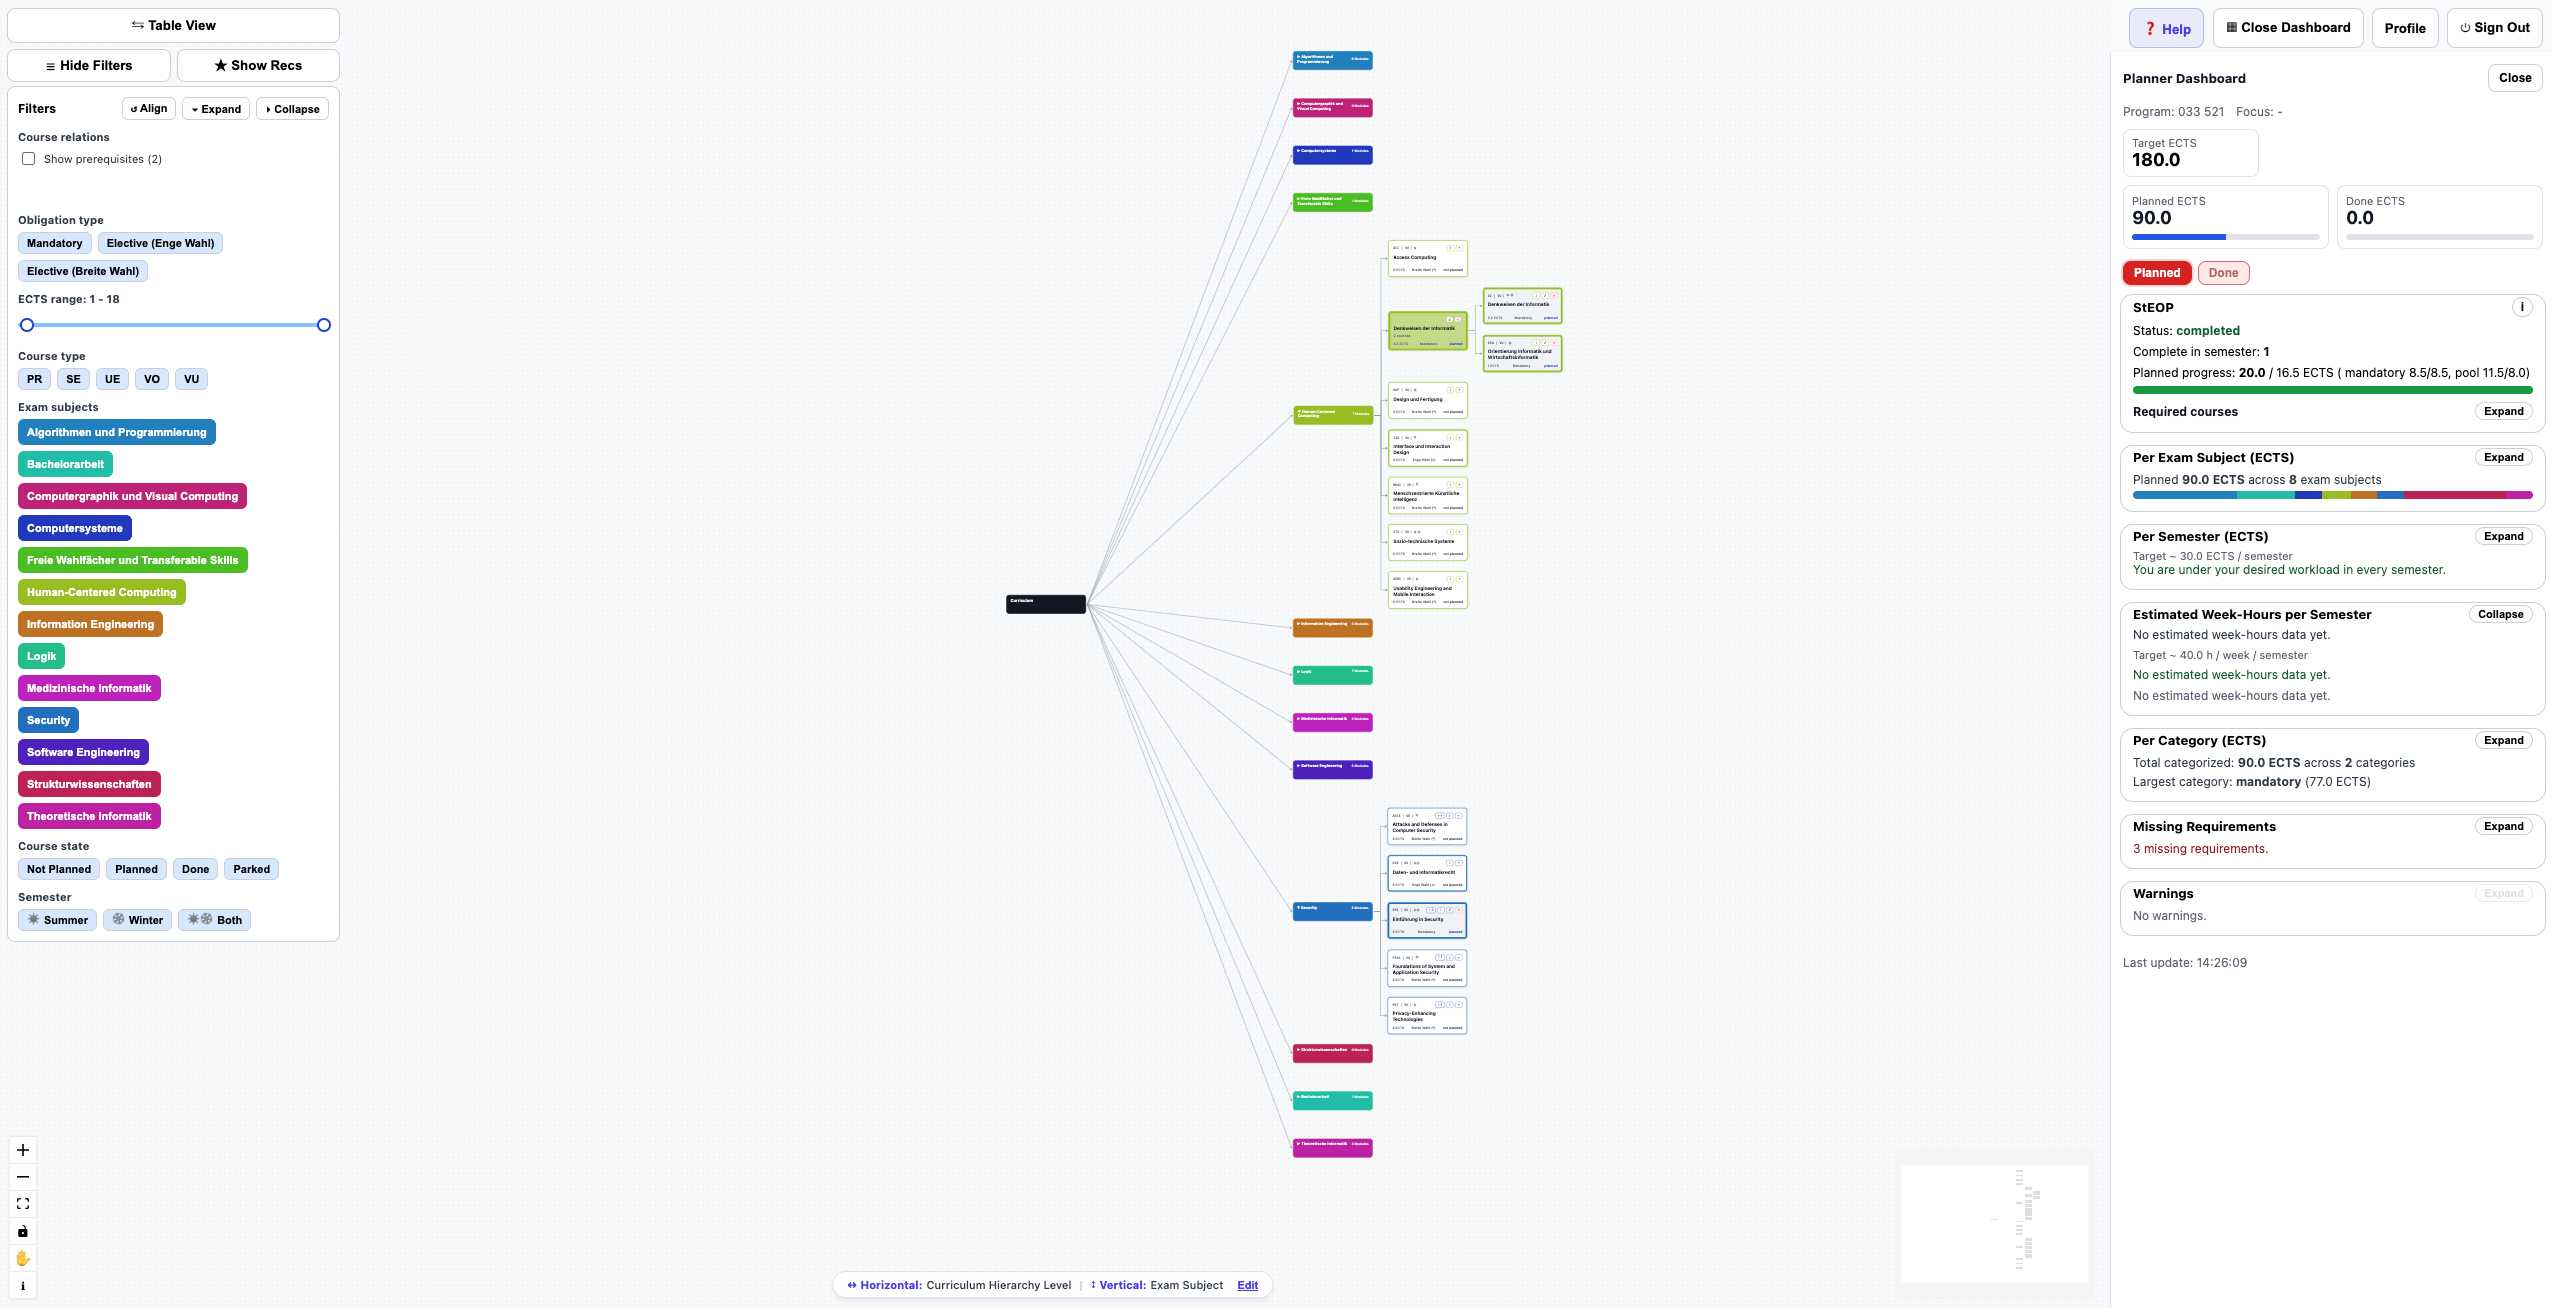
\includegraphics[width=\textwidth]{pictures/Full_graph_view_Screenshot.png}
\caption{The whole tool in the Graph View: the catalogue and its filters on the left, the curriculum in the centre, and the Dashboard on the right.}
\label{fig:impl-shot-shell}
\end{figure}

\begin{figure}[htbp]
\centering
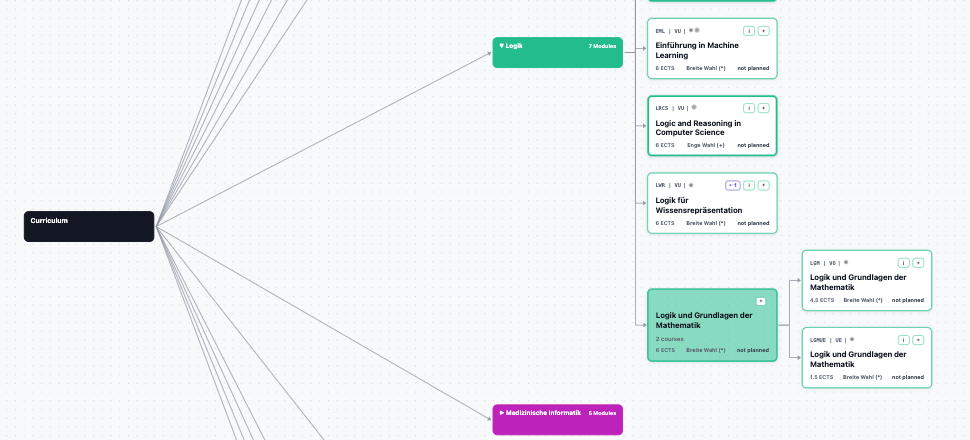
\includegraphics[width=\textwidth]{pictures/Graph_view_crop.png}
\caption{The Graph View, with all four levels in one frame: the programme root, an exam subject, its courses, and a module holding two courses drawn as its own node.}
\label{fig:impl-shot-graph}
\end{figure}

\begin{figure}[htbp]
\centering
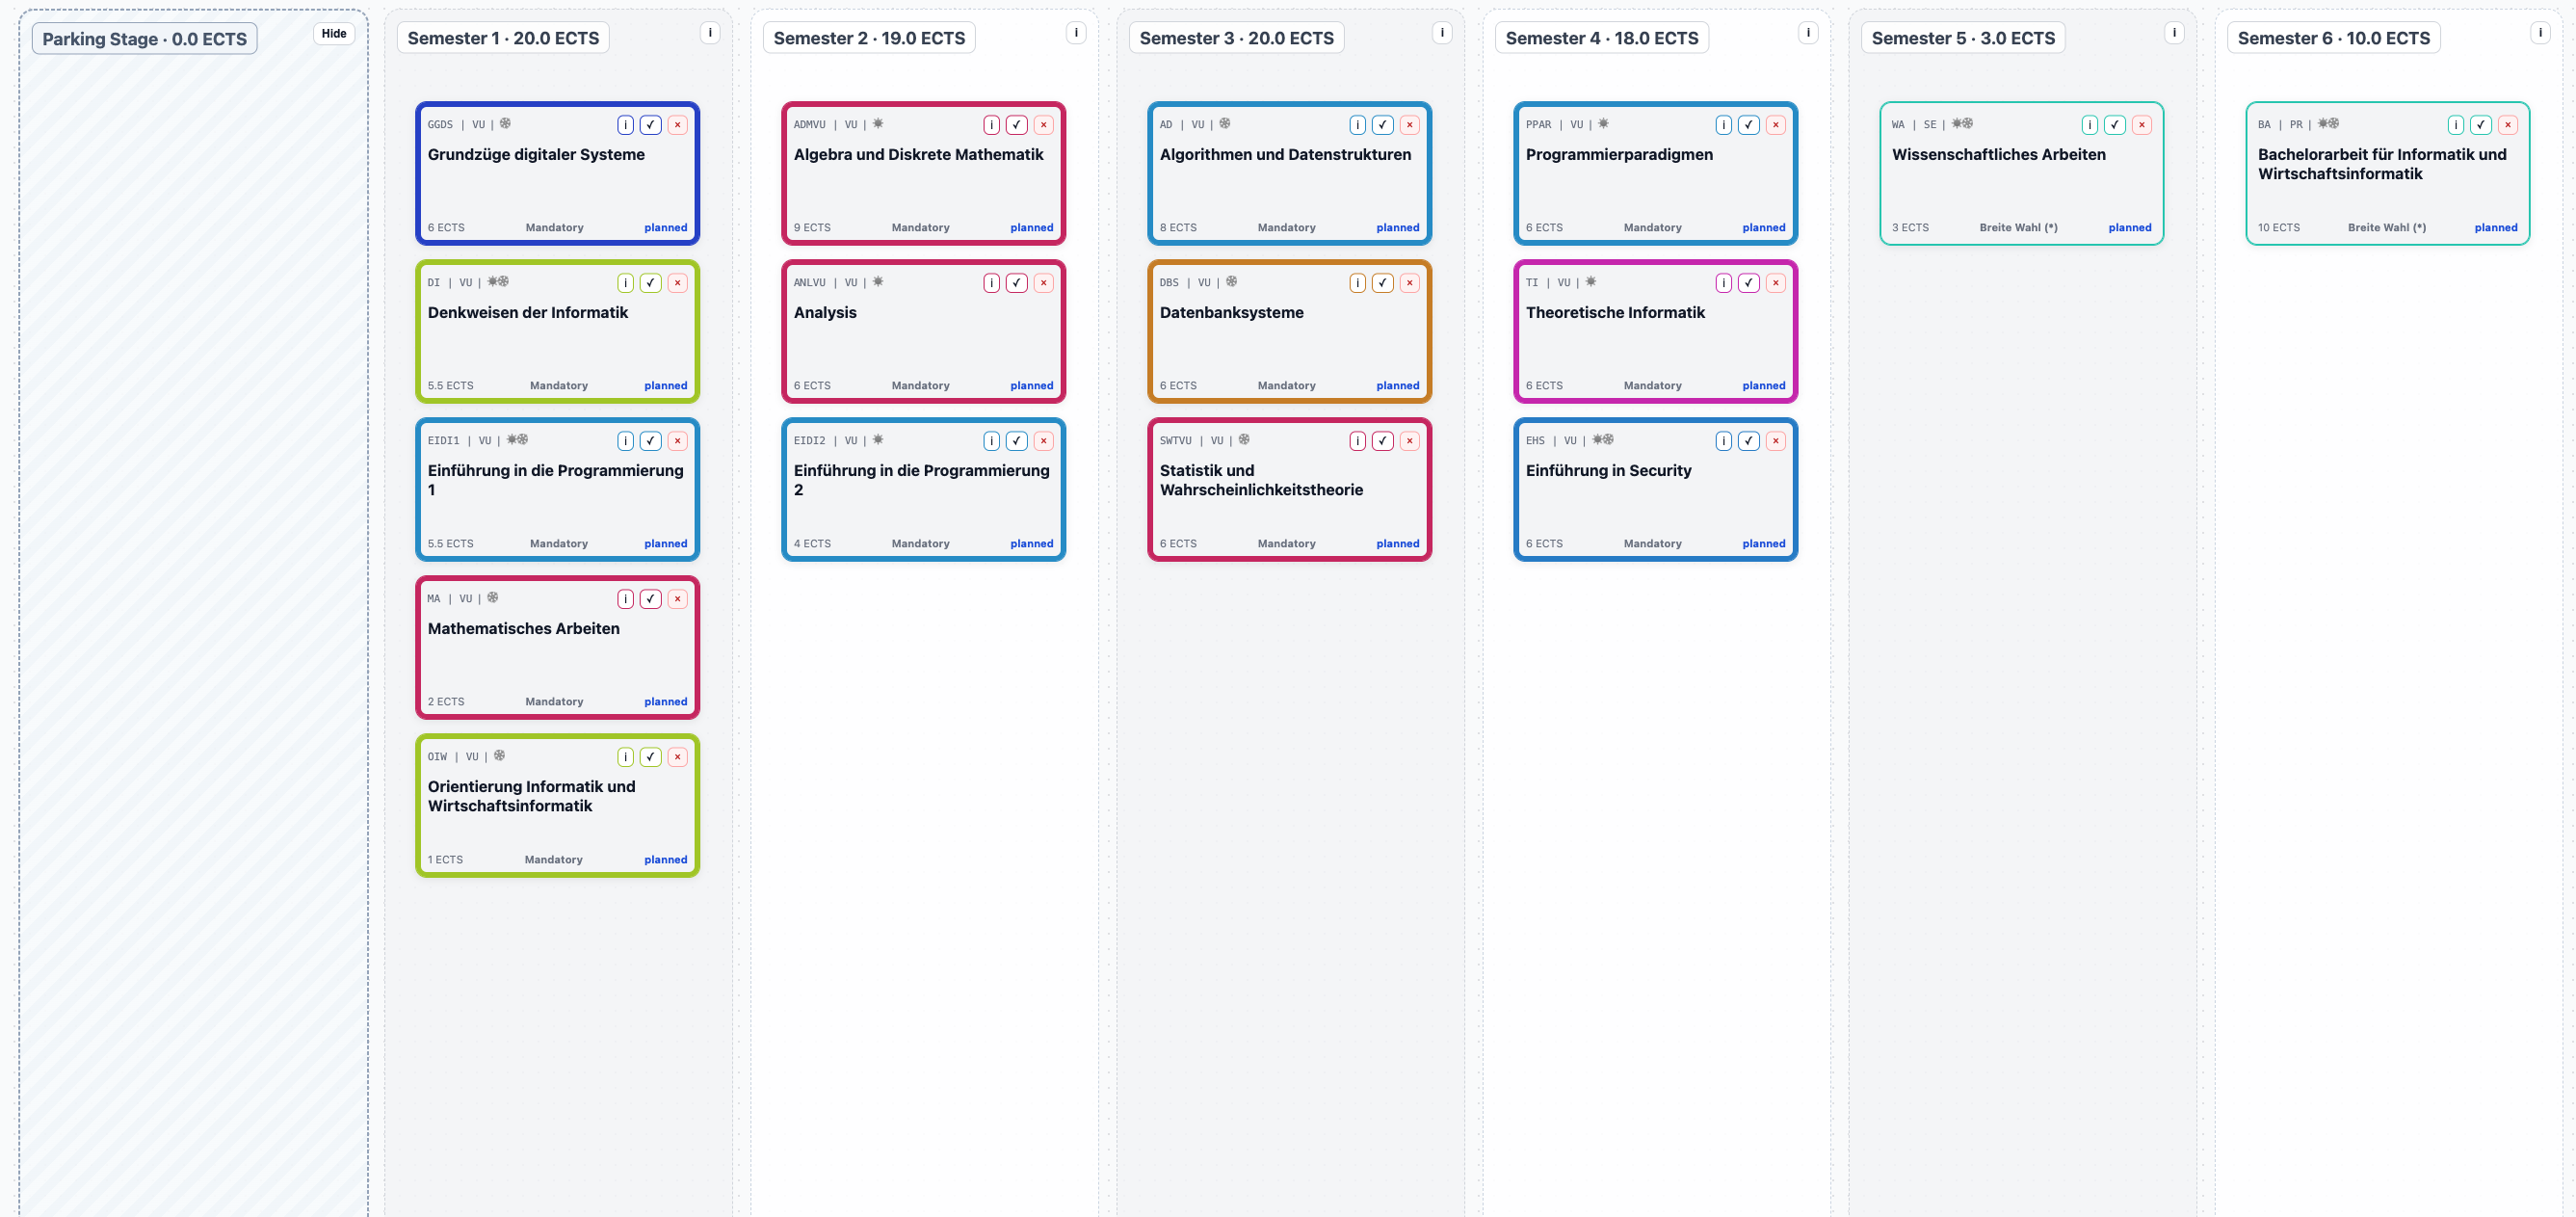
\includegraphics[width=\textwidth]{pictures/Table_Screenshot.png}
\caption{The Table View: the same plan arranged into semester lanes with their credit totals, and a Parking Stage on the left holding courses a student has shortlisted but not yet scheduled.}
\label{fig:impl-shot-table}
\end{figure}

\begin{figure}[htbp]
\centering
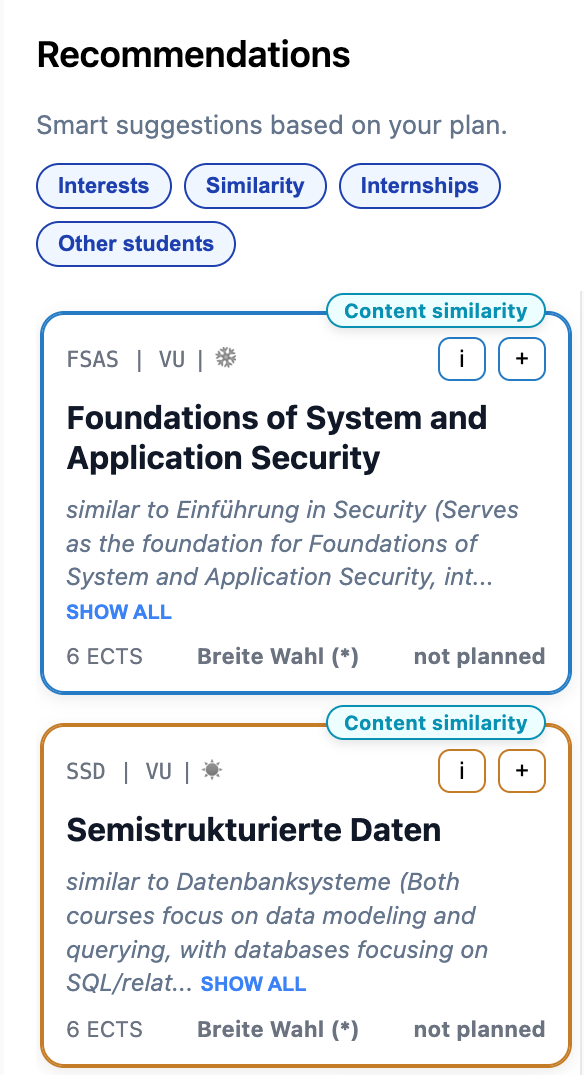
\includegraphics[height=8.6cm]{pictures/Recommendation_panel_crop.png}\hspace{6mm}%
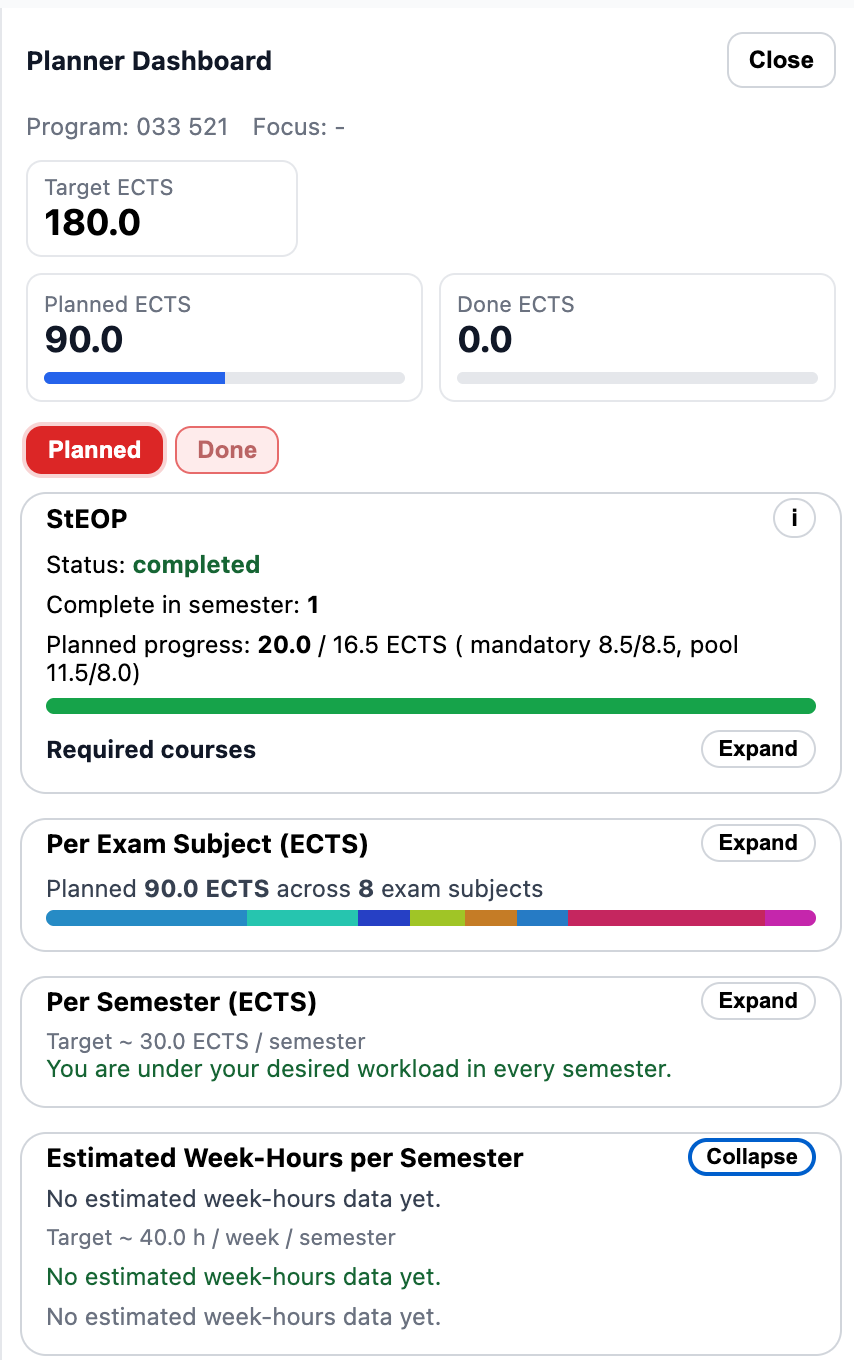
\includegraphics[height=8.6cm]{pictures/Dashboard_crop.png}
\caption{The two side panels: the Recommendation Panel, whose cards name the family that produced them, and the Dashboard, where the Compliance Engine's answer becomes visible. Both continue below the crop.}
\label{fig:impl-shot-recs}
\end{figure}

\begin{figure}[htbp]
\centering
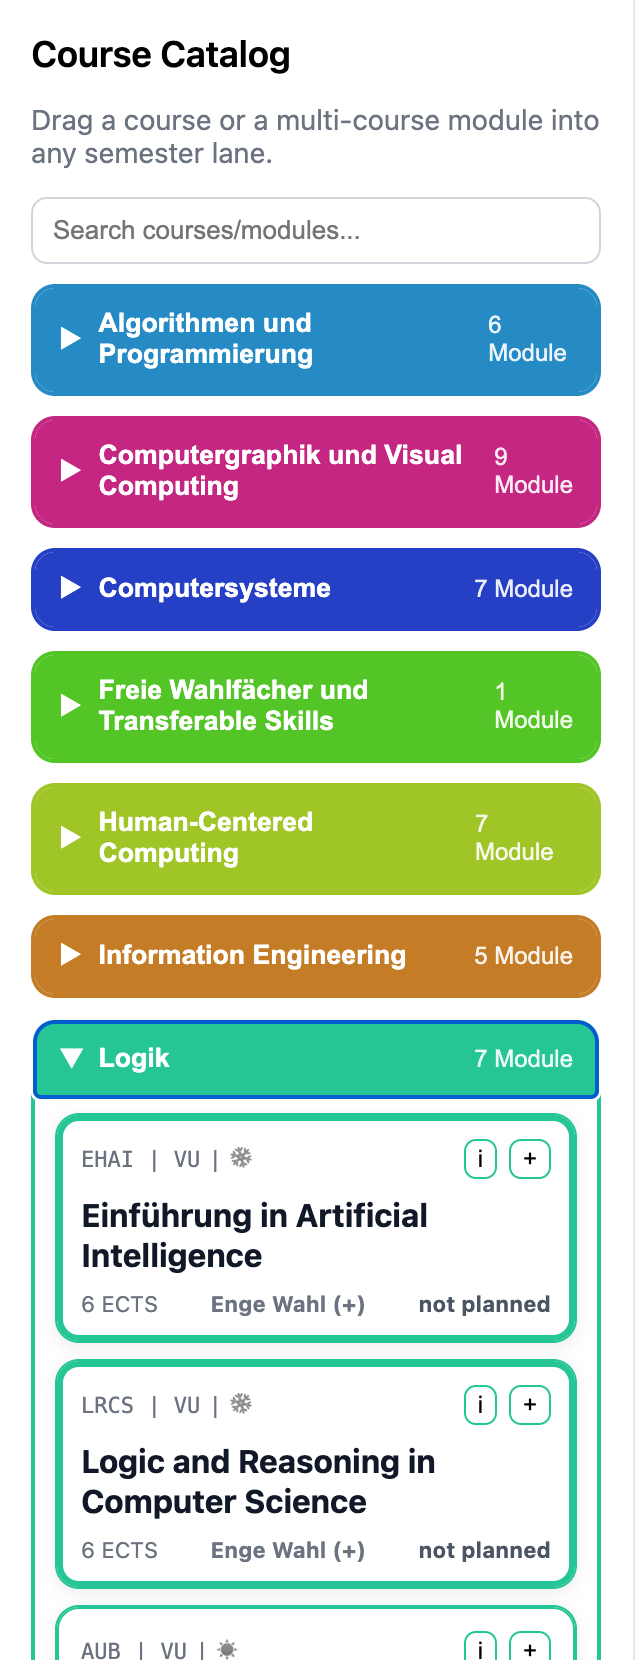
\includegraphics[height=8.4cm]{pictures/Sidebar_Screenshot.png}\hspace{6mm}%
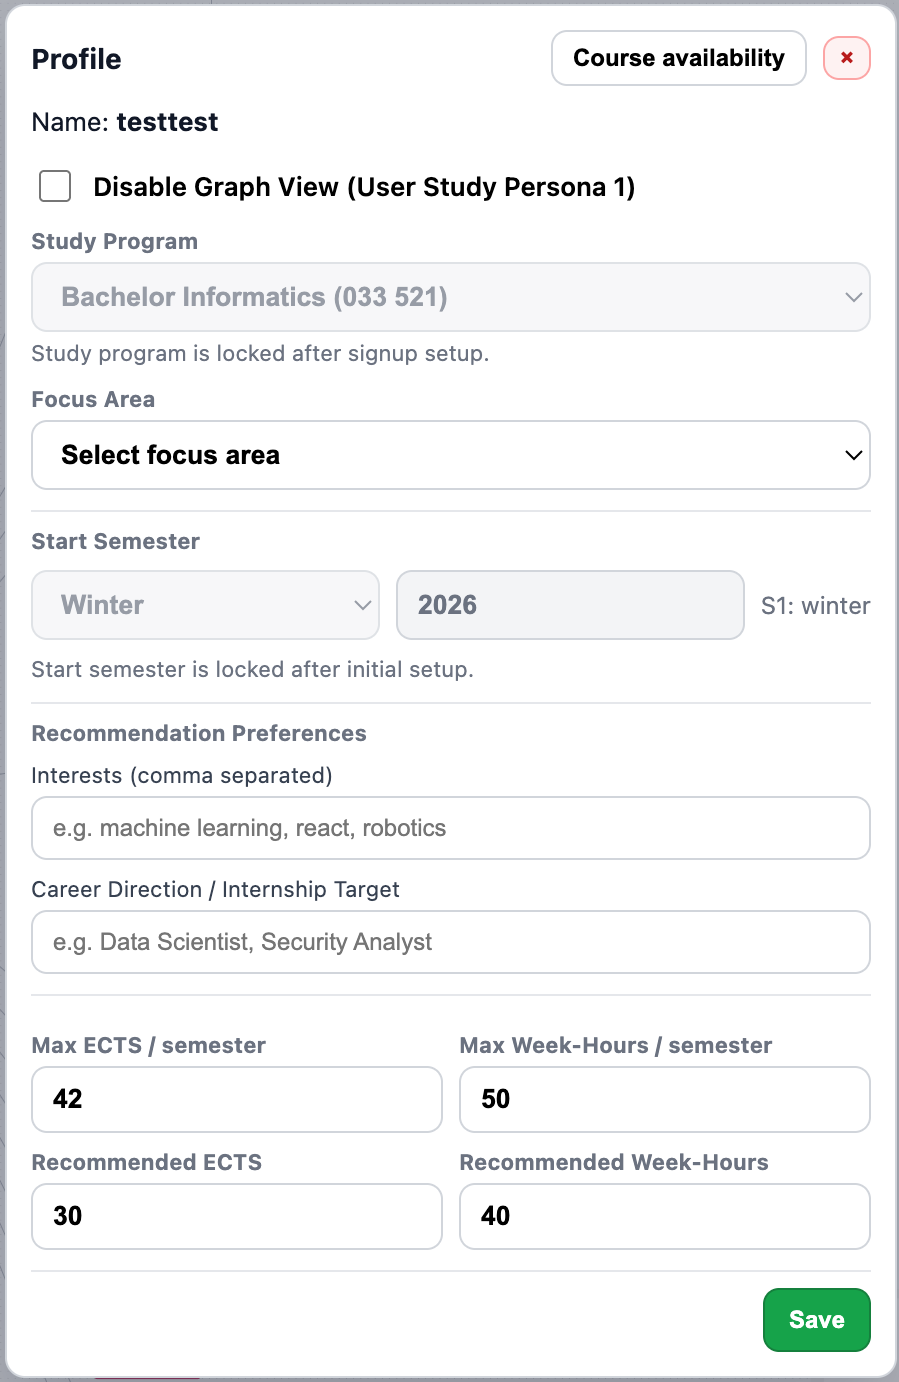
\includegraphics[height=8.4cm]{pictures/Profile__Screenshot.png}
\caption{The catalogue sidebar, grouped by exam subject with collapsible modules, and the profile dialogue holding the focus area, the recommendation preferences and the workload limits.}
\label{fig:impl-shot-catalogue-profile}
\end{figure}




\section{Backend}
\label{sec:impl-backend}

The backend service provides three functions: persistence of the study plan, curriculum compliance evaluation, and course recommendation. It is a FastAPI application structured in four layers with a strictly downward dependency direction (Figure~\ref{fig:impl-backend-components}). Request handlers validate input, invoke exactly one use case, and serialise the response; they contain no domain logic and no SQL. Use cases orchestrate domain operations and define the transaction boundary; eight service modules cover authentication and sessions, catalogue retrieval, prerequisite relations, plan persistence, profile settings, compliance evaluation, recommendation, and the capture of study results, which are stored as one file per questionnaire submission (Section~\ref{sec:impl-userstudy}). The domain layer comprises two packages, compliance and recommendation, described in Sections~\ref{sec:impl-compliance} and~\ref{sec:impl-recommender}. Repositories encapsulate all SQL statements.

Use cases access storage exclusively through a unit-of-work abstraction: an object that provides every repository bound to a single database connection. A use case therefore neither acquires connections nor references concrete repository classes. Two properties follow: a use case can be tested against a substitute unit of work without a database, and the set of statements that must commit atomically is declared in the use case rather than determined by repository execution order. Domain failures are raised as typed exceptions named for their cause, for instance \texttt{ProgrammeLocked}, \texttt{StartTermLocked} and \texttt{SetupIncomplete}; a single mapping table translates exception types to HTTP status codes and is the only component of the service aware of HTTP semantics. Authentication resolves the user from a session token supplied either as a cookie or as a bearer token, so that the deployed and the local client authenticate against an unchanged service. Persistence uses a shared PostgreSQL connection pool with parameterised SQL; no object-relational mapper is employed.

\begin{figure}[htbp]
\centering
\begin{tikzpicture}[font=\small,
  card/.style={draw, line width=1pt, rounded corners=3pt, fill=white, align=left, inner sep=2.5mm},
  wide/.style={card, text width=9.7cm},
  half/.style={card, text width=3.4cm, minimum height=13mm},
  a/.style={-{Latex[length=2.6mm]}, line width=1.1pt, draw=black},
  lb/.style={font=\scriptsize, inner sep=1.4pt, fill=white}]
  \node[wide] (api) {\textbf{Request handlers} \\[0.8mm] \small validate, call one use case, shape the reply};
  \node[wide, below=7mm of api] (svc) {\textbf{Use cases} \\[0.8mm] \small auth, catalogue, plan state, profile,\\ \small compliance, recommendation};
  \node[half, anchor=north west] (dom) at ($(svc.south west)+(0,-11mm)$) {\textbf{Compliance} \\[0.8mm] \small one rule set per programme, over the curriculum as data};
  \node[half, anchor=north east] (rec) at ($(svc.south east)+(0,-11mm)$) {\textbf{Recommendation} \\[0.8mm] \small six channels behind one protocol};
  \node[wide, anchor=north] (repo) at ($(dom.south)!0.5!(rec.south)+(0,-11mm)$) {\textbf{Repositories} \\[0.8mm] \small every SQL statement, bound to one connection by a unit of work};
  \coordinate (fork) at ($(svc.south)+(0,-5.5mm)$);
  \draw[a] (api) -- (svc);
  \draw[line width=1.1pt] (svc) -- (fork);
  \draw[a] (fork) -| (dom.north);
  \draw[a] (fork) -| (rec.north);
  \draw[a, rounded corners=2pt] (svc.west) -- ++(-11mm,0)
    |- node[lb, pos=0.45, anchor=east, xshift=-1.2mm] {reaches storage through} (repo.west);
  \draw[a] (rec.west) -- node[lb] {re-checks} (dom.east);
\end{tikzpicture}
\caption{Backend layers, under the same one-way dependency rule as the client: handlers hold no rules and no SQL, use cases own the transaction boundary, and the recommender re-checks every suggestion.}
\label{fig:impl-backend-components}
\end{figure}

\subsection{Curriculum Compliance Engine}
\label{sec:impl-compliance}

The Compliance Engine implements Feature~\ref{feat:003} and Feature~\ref{feat:005}. All rules are derived from the published curricula of the two supported programmes, the Bachelor programme in Computer Science and the Master programme in Software Engineering\footnote{\url{https://informatics.tuwien.ac.at/bachelor/curriculum-ue033521.pdf}, \url{https://informatics.tuwien.ac.at/master/curriculum-ue066937.pdf}; the versions in force during this work were used.}; no rule has another source.

Curriculum content is separated from evaluation logic. Each programme's regulations are encoded as a JSON document in \texttt{app/curriculum/}, comprising modules and credit weights, the course-to-module mapping, the introductory-phase course sets, focus areas with their aliases, prerequisite pairs, and numeric thresholds (nine constants for the Bachelor programme, five for the Master). The two documents do not share a schema: the Master document contains no course-to-module mapping, focus areas or introductory phase, as its curriculum defines none. Each checker loads its document once at construction; a curriculum revision therefore modifies data, not code.

Evaluation is performed by one rule set per programme, selected by programme code. The two rule sets share only the request format, the result schema, the entry point and the interpretation of credit limits. The Bachelor rule set enforces the introductory phase (\gterm{steop}{StEOP}); the Master rule set enforces its prerequisite pairs and emits a warning when the electives of an exam subject precede its core modules; neither rule has a counterpart in the other curriculum. No common base class was introduced, since the shared logic is smaller than the abstraction required to express it; whether a common core emerges with a third programme is left to future work.

For a submitted plan, the engine computes credit totals per semester and per exam subject and evaluates them against the curriculum: semester load against the absolute ceiling and the recommended load, module completeness and exam-subject minima, prerequisite and sequencing rules, and the total credit requirement. Findings are classified in two tiers, so that the interface guides rather than blocks (Section~\ref{sec:overall-scope}). An error, for instance a semester exceeding its ceiling or a violated hard prerequisite, rejects the triggering change, which the client reverts; a warning, for instance a semester exceeding its recommended load or an elective scheduled before its subject's core modules, is advisory. The result additionally carries the statistics rendered by the Dashboard, so that interface and rule engine derive from a single computation. The recommendation engine invokes the same checker to validate every candidate suggestion (Section~\ref{sec:impl-recommender}).

\subsection{Recommendation Support}
\label{sec:impl-recommender}

The recommendation component implements the recommendation workflow of the design (Feature~\ref{feat:007}, Feature~\ref{feat:012}). It is not a contribution to recommender-systems research, and the accuracy of its methods is excluded from scope by OOS5. It combines established techniques: content-based matching against stated interests and curated course similarities, sequence relations of the kind proposed by sequence-based course recommenders~\cite{wong_sequence_2018}, and a collaborative-filtering component modelled on elective recommendation~\cite{bhumichitr_recommender_2017}. The collaborative component operates on a synthetically generated cohort of prior-student plans rather than on real interaction data; it therefore reproduces the workflow of a data-driven recommender, not its performance.

Six channels implement a common protocol consisting of a name and a single scoring method that returns a score and an evidence string for a candidate course. The interest channel weights an explicit topic match above a description match and a partial keyword overlap below both, normalised by the number of stated interests. The similarity channel performs no inference; it reads curated course-to-course links stored in the catalogue, each carrying the justification presented as evidence (Figure~\ref{fig:impl-shot-recs}). The sequence channel reads the orderings the curricula define between named courses. The follow-on channel scores a candidate by the proportion of cohort members who took it after a course the student has completed and suppresses proportions below a majority; the peer channel scores it by the proportion among the cohort members whose plans most overlap the student's, and reverts to overall popularity, flagged as such, for an empty plan. The internship channel matches the stated career direction against course skills and descriptions. The engine queries the channels in a fixed order, retains one record per course, sorts by score, and validates each of the top hundred records against the Compliance Engine by trial placement, discarding any record that would introduce an error or a warning absent from the baseline evaluation; at most fifteen records are returned. Since scores are assigned per channel, a channel with a fixed high score, such as curated similarity, dominates the top of the list.

All six families were active during the sessions reported in Chapter~\ref{chap:evaluation}. Four depend on student-supplied data or on the synthetic cohort and return no results without input: a participant who entered no interests received no interest matches, which partly explains the empty recommendation tab recorded as E-P42. The sequence family is bounded by the curricula: the Bachelor curriculum defines two orderings, the same sparsity the graph overlay exhibits, which accounts for four of the eleven participants requesting ordering information without obtaining it (E-P44). The evaluation examines how students work with recommendations presented in this form, not the accuracy of the matching; the requirements of a production version with real, consented interaction data are stated with the limitations.

\section{Data Model}
\label{sec:impl-data}

The database represents a programme as a strict four-level hierarchy (Figure~\ref{fig:impl-data-model}): programme, exam subject, module, course. In both catalogues each course belongs to exactly one module; this property holds in the seeded data and is not enforced by the schema. A materialised view projects the catalogue of each programme into a single nested JSON document, which the client retrieves in one request; the service merges the student's term-availability overrides into this document before responding, so that shared catalogue data is never modified by user actions. Course metadata that evolves independently of the relational schema, namely content descriptors and curated course similarities, is stored in a JSONB attributes column of the course table.

Per-user data consists of the account, one saved plan, and one profile per programme. The plan table is keyed by user and written by upsert, so each account holds exactly one plan; the profile table is keyed by user and programme, so a student who changes programme retains a profile for each. No foreign key links the per-user tables to the catalogue: programmes and courses are referenced by code, so a plan remains valid when the catalogue is reseeded and its identifiers regenerated. A single plan per account was sufficient for the study but precludes parallel alternative drafts, a limitation discussed in Chapter~\ref{chap:discussion} (Section~\ref{sec:disc-future}).

The schema is constructed by migration files applied in lexical order at service start-up. Files are named by timestamp rather than by sequence number to avoid collisions under concurrent development; each applied file is recorded with a checksum, and a modified file aborts start-up; down-migrations are not provided.

\begin{figure}[htbp]
\centering
\begin{tikzpicture}[font=\small,
  ent/.style={draw, line width=1pt, rounded corners=3pt, fill=white, align=center, inner sep=2.2mm, text width=2.9cm},
  rel/.style={draw=black, line width=1.2pt, -{Latex[length=2.5mm]}},
  proj/.style={draw=black!60, line width=1pt, dashed},
  lbl/.style={font=\scriptsize, fill=white, inner sep=0.8pt}]
  \node[ent] (sp) {\textbf{study\_program}};
  \node[ent, below=9mm of sp] (es) {\textbf{exam\_subject}};
  \node[ent, below=9mm of es] (mo) {\textbf{module}};
  \node[ent, below=9mm of mo] (co) {\textbf{course}\\ \footnotesize +\,JSONB attributes};
  \coordinate (spine) at ($(sp.west)+(-8mm,0)$);
  \coordinate (spineb) at ($(co.west)+(-8mm,0)$);
  \coordinate (spinemid) at ($(spine)!0.5!(spineb)$);
  \node[ent, dashed, left=8mm of spinemid] (mv) {\footnotesize materialised\\ \footnotesize catalogue view};
  \draw[rel] (sp) -- node[lbl]{1\,:\,N} (es);
  \draw[rel] (es) -- node[lbl]{1\,:\,N} (mo);
  \draw[rel] (mo) -- node[lbl]{1\,:\,N} (co);
  \draw[proj] (spine) -- (spineb);
  \foreach \n in {sp,es,mo,co} {\draw[proj] (\n.west) -- (\n.west -| spine);}
  \draw[proj, -{Latex[length=2.5mm]}] (spinemid) -- (mv.east);
  \node[ent, right=17mm of sp] (au) {\textbf{app\_user}};
  \node[ent, below=7mm of au] (ps) {saved plan};
  \node[ent, below=7mm of ps] (pp) {programme profile};
  \draw[rel] (au) -- node[lbl]{1\,:\,1} (ps);
  \draw[rel, rounded corners=2pt] (au.east) -- ++(9mm,0) |- node[lbl, pos=0.75]{1\,:\,N} (pp.east);
\end{tikzpicture}
\caption{Data model. The catalogue (left) is projected per programme into a materialised JSON view; per-user data (right) is one plan document per account and one profile row per programme.}
\label{fig:impl-data-model}
\end{figure}

\section{Evaluation Instrument}
\label{sec:impl-userstudy}

The evaluation sessions (Chapter~\ref{chap:evaluation}) were run with a small, standalone questionnaire web application, kept deliberately separate from the study planner so that instrumentation could not affect the tool under study. It guides a session through consent, demographics, the task scenarios, and the post-task questionnaire, keeps its own timers, and submits each session's responses for later analysis. The instruments themselves and the study they support are described in Chapter~\ref{chap:evaluation}; the application is noted here only as a distinct artefact produced for this work.

\section{Verification}
\label{sec:impl-verification}

Munzner's nested model attaches its own threat, and so its own form of validation, to each level, and warns that a poor result at one level may in fact be caused by a poor choice at a level inside it~\cite[p.~922]{munzner2009}. The algorithm level is this chapter's, and verifying it here is what allows Chapter~\ref{chap:evaluation} to read a usability result as a statement about the design rather than about a defect underneath it. We focus verification on the Compliance Engine, as both user trust and the evaluation findings depend entirely on its correctness, and verify the system across three levels.
First, a test suite records the engine's exact output across 38 scenarios for both degree programmes, covering empty plans, boundary conditions, and deliberate rule violations. We compare every verdict and statistic field by field to pinpoint specific rule failures. The corpus itself is guarded: the builder refuses to record a set of scenarios whose answers are less than half distinct, so the suite cannot pass by comparing a uniform corpus with itself. We apply this same snapshot strategy to the recommender system across 85 distinct profile and channel configurations.
Second, contract tests verify the API surface. We sanitise dynamic values, such as timestamps and identifiers, to strictly assert that endpoint status codes and response structures remain stable across runs.
Third, end-to-end tests drive a browser against the running stack to simulate the core planning loop. This is necessary to verify the two-way reconciliation between the plan model and the interface canvas (Section~\ref{sec:impl-frontend}), which cannot be observed outside a real browser environment.
Standard unit tests cover the remaining components. Client-side tests isolate the domain layer, including the plan reducer and graph filters. Service-side tests cover the curriculum documents, individual recommendation channels, catalogue queries, and database migration integrity. A continuous integration pipeline runs this entire suite alongside strict type checks on every change.
This heavy reliance on recorded verification is effective here because the Compliance Engine is strictly deterministic and the plan model is a pure function of its inputs, guaranteeing stable test outputs for any given state.

% =============================================================================
\section{Revisions After the Evaluation Study}
\label{sec:impl-post-study}

Everything described up to this point is the system used in the evaluation study of Chapter~\ref{chap:evaluation}. This section records what was changed afterwards, and it is kept separate for exactly that reason: none of it was in front of a participant, and no finding in Chapter~\ref{chap:evaluation} may be read as evidence about it. The changes fall into two kinds. The first is a set of corrections to defects the study surfaced (Section~\ref{sec:impl-post-study-fixes}). The second is an addition rather than a correction, the soft-dependency edge layer (Section~\ref{sec:impl-prereq-edges}), which supplies a capability four of the eleven participants asked for and did not receive (E-P44, 4/11).

\TDrev{The post-study corrections section is far too long}{Your comment, deferred with the note above, 2026-09-05: how far this can be cut depends on which corrections survive, and that is settled after Chapters~\ref{chap:evaluation} and~\ref{chap:discussion}. The intended shape is a short statement that the defects closed after the study were closed with a regression test each, with the ticked column of Table~\ref{tab:problems} doing the enumerating, plus one sentence on why those and not others. The soft-dependency edge layer stays as its own subsection, since it is an addition rather than a correction.}
\subsection{Corrections to Reported Defects}
\label{sec:impl-post-study-fixes}

The defects of Table~\ref{tab:problems} are held as a register in the tool's repository, ranked by the severity and frequency reported in Chapter~\ref{chap:evaluation}. Five have been closed, each with a regression test that reproduces the observed failure before the fix and passes after it. The remainder are open and are not discussed here.

\TDrev{Deferred: which defects were closed after the study, and what the register says}{Deferred by decision, 2026-09-05, until Chapters~\ref{chap:evaluation} and~\ref{chap:discussion} are settled, because the list can still grow: further defects may be fixed before submission. What is known now, from the code check of 2026-09-05: the study's E-P codes appear in the tool's repository only in its register of problems, none marked closed; no test names any of them; and the panel's empty state is a generic \enquote{No recommendations} rather than the per-tab explanation described below. Two of the five also sit oddly with the author's own account of the sessions, that E-P29's term marker was on every course card before the study and that E-P42's tabs worked during it. When this is taken up, settle the register first, then scope this sentence and the ticked column of Table~\ref{tab:problems} to exactly what is merged.}

Term availability (E-P29) was legible only through a filter dimension, not from a course card. A winter or summer marker was added to the card in both views and to the catalogue row, drawing on the same field the filter already used.

The feedback banners failed in two independent ways and both were corrected (E-P50, and the arithmetic half of E-G09). One visual style carried acceptance, rejection and progress, so a refusal could not be told from a confirmation; the three now have distinct styles, and a rejection states the constraint that produced it. Separately, milestone banners computed their percentage against a hard-coded credit denominator rather than the loaded programme's own total, which is what produced the runs announcing 25\,\% completion at 102 and at 108 of 180~ECTS; the denominator now comes from the curriculum in force.

The internships and interdisciplinary recommendation tabs rendered a bare dead end when a channel returned nothing (E-P42). A tab with no candidates now states why it is empty. This does not repair the underlying cause, which is the placeholder interaction data described in Section~\ref{sec:impl-recommender}; it stops the empty state from reading as a fault in the tool.

The profile screen carried wording written for the study rather than for a student (E-P27), which was rewritten.

The fifth correction is the edge layer, and it is large enough to take separately.

\subsection{The Soft-Dependency Edge Layer}
\label{sec:impl-prereq-edges}

The evaluated graph already drew the formal prerequisite pairs the two curricula fix, as a togglable overlay on the containment layout (Chapter~\ref{chap:design}, Section~\ref{sec:graph-ltr}). What it did not draw was the other half of the relation the Compliance Engine holds: the soft, recommended orderings the engine reports as non-blocking Dashboard advisories (Section~\ref{sec:impl-compliance}; Feature~\ref{feat:003}, Req.~3). That asymmetry was a design decision rather than a limit of the data. The overlay was scoped from the outset to the relations the Compliance Engine blocks on, so that an edge in the graph would carry one meaning, this ordering is required, and a student would not have to ask of any given edge whether it was binding. The evaluation showed the cost of that choice: four of the eleven participants asked for ordering information at the point of placement and did not receive it (E-P44, 4/11), and no other view offered it either. The layer added afterwards therefore widens the overlay rather than acquiring anything new, drawing the recommended orderings the curricula themselves state, as notes on the prior knowledge a course expects, alongside the pairs they fix.

The layer reuses the mechanism the formal edges already use. The soft pairs, which live as an attribute of each programme's checker class (Section~\ref{sec:impl-compliance}), are now served alongside the catalogue instead of remaining inside the engine, and the graph renders them as a second edge style: dashed where the formal edges are solid, and labelled \emph{recommended before} where the formal edges read \emph{required before}, so the two are told apart on the canvas rather than through a legend. Both kinds answer to one switch in the filter sidebar, which draws them together or not at all, so the overlay can be cleared in a single action, which is what the decluttering requirement asks for (DEP-04). Because both edge types cross the exam-subject bands rather than running along them, they are drawn above the containment layout and are hidden by default; node positions are unchanged, so the spatial memory the design protects (Feature~\ref{feat:013}, Req.~2) survives turning the overlay on and off.

The layer was built after the study, so no participant used it and Chapter~\ref{chap:evaluation} carries no evidence about how it is read. And what the switch draws is thin by construction: the relations the curricula fix between two named courses are two advisory pairs in the Bachelor programme and two enforced ones in the Master, a handful of edges over a graph of 84 courses. The expected-knowledge orderings are 99 edges in the Bachelor programme and 24 in the Master, but they are never drawn together: they appear around a single node, on request, which is what keeps them from returning the graph to the density the collapse controls exist to manage. Chapter~\ref{chap:discussion} (Section~\ref{sec:disc-future}) takes up what would have to be established before a view of this kind, drawing dependencies and soft dependencies together, could be said to earn its place.

% =============================================================================
\section{Key Decisions}
\label{sec:impl-decisions}
Four decisions shaped what the evaluation was able to observe, and it is that consequence rather than the rationale already given above that is worth drawing together here.

The single authoritative plan model (Section~\ref{sec:impl-frontend}) is what made the two-condition design possible at all. Because both views are projections of one plan, turning the graph off removes a projection rather than a data path, so the graph-off condition is the same tool with one surface withdrawn and not a second tool that has to be trusted to behave identically. The substitution result of Chapter~\ref{chap:evaluation} rests on that: the catalogue and the graph could exchange places in the workflow precisely because neither owned the plan.

Holding each programme's regulations apart from the logic that evaluates them (Section~\ref{sec:impl-compliance}) is what let the study use two curricula and one instrument. The Bachelor programme's rules drove every session reported here while the Master's remained available and unchanged, which is why the completion audit can be read as a statement about plans rather than about which rule set happened to be loaded.

The deliberate simplicity of the recommendation component (Section~\ref{sec:impl-recommender}) determined what the recommendation findings can mean. Because the channels combine standard techniques over placeholder data, the study observes how students treat an explainable suggestion rather than how good the suggestions are, and the expertise-moderated pattern the Discussion reports is a finding about the workflow that survives whatever a better ranking would have produced. The same decision is why two channels were inert during the study, which bounds that finding in the opposite direction.

Verifying the Compliance Engine by recording its answers rather than asserting propositions about them (Section~\ref{sec:impl-verification}) is what makes the evaluation's central negative result checkable. When Chapter~\ref{chap:evaluation} reports that the tool certified plans breaching constraints it does not model, that is a statement about the engine's scope and not a suspicion about its correctness, because the recorded corpus shows the engine answering consistently for the rules it does hold. A test suite restating the curriculum as propositions could not have separated those two possibilities, since a misreading of the curriculum would have appeared identically in the rules and in the tests meant to check them.






\chapter{Evaluation}
\label{chap:evaluation}
This chapter answers Research Question~3:

\begin{quote}
\textit{How do students plan with the hybrid interface, and what does the graph-based view contribute to their planning?}
\end{quote}

It reports the evaluation study: the study's goal and the questions that guided it (Section~\ref{sec:eval-design}), the system as the artefact under evaluation (Section~\ref{sec:eval-system}), the participants (Section~\ref{sec:eval-participants}), the procedure (Section~\ref{sec:eval-procedure}) and the analysis method (Section~\ref{sec:eval-analysis}), then the findings (Section~\ref{sec:eval-results}), which Chapter~\ref{chap:discussion} interprets. In the terms of the nested model, the study validates the encoding, interaction and algorithm levels of the artefact~\cite{munzner2009}.

\section{Study Goal and Guiding Questions}
\label{sec:eval-design}

The study investigates how a curriculum graph alters the planning process of students equipped with an established tabular workflow. While the formative study treated the graph view's utility as a premise (Section~\ref{sec:overall-assumptions}) and conceptually partitioned the interface into exploratory (graph) and commitment-oriented (table) modalities (Section~\ref{sec:mutual-exclusion}), neither assumption had undergone evaluation. We therefore conducted a within-subjects observational study ($N=11$) where participants completed comparable planning tasks using the system of Chapter~\ref{chap:implementation} first with the tabular baseline alone, then with the graph view enabled. Granular, frame-by-frame behavioral logging paired with participant reports allows the graph's operational contribution to be traced directly within the planning process. This focus on process tracing governed the research design. Detecting reliable outcome differences in speed or plan quality would require a high-powered, counterbalanced sample matched for domain knowledge; we deliberately prioritized observational fidelity over broad generalization. Across 22 recorded sessions, frame-level coding generated descriptive findings and grounded hypotheses. We used a fixed condition order intentionally within this framing; its methodological trade-offs were anticipated (Section~\ref{sec:eval-order}), and no empirical claims in this chapter depend on comparative inferences that could be compromised by order effects.

\subsection{Guiding Questions}
\label{sec:eval-guiding}

To operationalise this goal, the study was guided by four questions, carried over from the proposal for this thesis, which planned a task-based evaluation of the hybrid interface and of the recommendations embedded in it:

\begin{itemize}
    \item \textbf{Planning practice:} How do students execute the planning process using the tool?
    \item \textbf{The graph's contribution:} What does the graph-based view add to that work? Answered by comparing the two conditions within each participant (Section~\ref{sec:eval-ab}).
    \item \textbf{Recommendations in the workflow:} Where and how do the embedded recommendations help?
    \item \textbf{Outcomes and satisfaction:} Do the plans students produce meet the task they were set, and how satisfied are students with the tool?
\end{itemize}

\subsection{Scope and Non-Goals}
\label{sec:eval-nongoals}

This study does not evaluate plan accuracy or generation speed, nor does it use either to compare the two conditions. Establishing reliable outcome measures would require matched cohorts with a known baseline of curriculum knowledge, a tool-agnostic operationalization of plan quality, and a sample large enough to isolate condition effects from individual variance. These prerequisites fall outside the scope of a qualitative, small-scale observational design. The completion audit in Section~\ref{sec:eval-effectiveness} is therefore not a performance comparison. It serves a single methodological purpose: by independently establishing which plans met the brief, it reveals the gap between perceived and actual success, thereby contextualizing the self-reported data.

\section{System as Evaluation Artefact}
\label{sec:eval-system}

The evaluated system is the tool detailed in Chapters~\ref{chap:design} and~\ref{chap:implementation}. To provide context for the analysis codes, the components carrying the findings are: the Table View (Section~\ref{sec:table-view}), the Graph View with its filter sidebar and prerequisite overlay (Section~\ref{sec:graph-spatial}), the Dashboard (Sections~\ref{sec:dashboard} and~\ref{sec:compliance}), the Recommendation Panel (Section~\ref{sec:rec-panel}), the Parking Stage (Section~\ref{sec:parking}), the Course Catalogue (Section~\ref{sec:sidebar-design}), the visual legend (Section~\ref{sec:legend}), and the onboarding tour (Section~\ref{sec:onboarding}).

\section{Participants and Recruitment}
\label{sec:eval-participants}
%% REV (is this kind of table with the participants missing in chapter 4?)
Twelve sessions were conducted and eleven are analysed. One session (P08) was excluded due to a lack of consent for the screen recording, which precluded the visual analysis method detailed in Section~\ref{sec:eval-analysis}.

Participants were recruited from the Faculty of Informatics at TU~Wien through the author's network. Eligibility was restricted to students enrolled in one of the two target programmes; no compensation was provided. The eleven analysed participants ranged from their 2nd to 8th semester across Software Engineering (MSc) and Computer Science (BSc), and they span the target experience strata: four reported regular prior experience with study-planning tools, one reported little, and six reported none (Table~\ref{tab:participants}). No recording frames are reproduced in this thesis, and participants are referred to exclusively by assigned codes.

\begin{table}[htpb]
    \centering
    \small
    \begin{tabular}{llcl}
        \toprule
        P & Programme & Sem. & Prior exp. \\
        \midrule
        P01 & Software Engineering (MSc) & 6 & none    \\
        P02 & Software Engineering (MSc) & 6 & regular \\
        P03 & Computer Science (BSc)     & 6 & none    \\
        P04 & Software Engineering (MSc) & 5 & regular \\
        P05 & Software Engineering (MSc) & 8 & none    \\
        P06 & Software Engineering (MSc) & 2 & none    \\
        P07 & Software Engineering (MSc) & 8 & regular \\
        P09 & Software Engineering (MSc) & 5 & little  \\
        P10 & Computer Science (BSc)     & 2 & none    \\
        P11 & Computer Science (BSc)     & 2 & none    \\
        P12 & Software Engineering (MSc) & 6 & regular \\
        \bottomrule
    \end{tabular}
    \caption{The eleven analysed participants. P08 is excluded and not listed.}
    \label{tab:participants}
\end{table}

\section{Procedure}
\label{sec:eval-procedure}

Each participant used the tool under two conditions in a fixed order during a single session. This section details the conditions and their task briefs, the rationale for the fixed order and its methodological trade-offs, and the session sequence alongside its measurement instruments.

\subsection{Conditions and Scenarios}
\label{sec:eval-conditions}

Each participant completed two planning tasks under different graph availability settings. To control for individual domain preferences, these tasks were framed as persona scenarios. The graph setting was an account-level property fixed before each task began; participants could not toggle the view on or off during a scenario.

\begin{itemize}
    \item \textbf{Scenario~A (graph off).} A Cybersecurity persona, planned with the graph unavailable. The table, Dashboard, recommendations, catalogue, and Parking Stage remain fully available.
    \item \textbf{Scenario~B (graph on).} An Artificial Intelligence persona, planned with the full tool including the graph and its filter sidebar.
\end{itemize}

Everything other than graph availability was held constant across the two conditions. Each brief stated only its persona constraints, namely the per-semester ECTS band and the single reduced-load semester, along with strategic guidance on preferred module types. The curriculum's inherent hard requirements (the mandatory modules, the chosen focus area, the narrow (\emph{enge Wahl}) and broad (\emph{breite Wahl}) electives, and the introductory-phase (StEOP) rules) were intentionally excluded from the brief. Participants encountered these only inside the tool and tracked them via the Dashboard, making the Dashboard the sole channel through which curriculum constraints were communicated during a task. The two briefs are reproduced exactly as presented in %% REV (this is not a section isnt it?) 
Section~\ref{app:eval-scenarios}.

\subsection{Fixed Scenario Order}
\label{sec:eval-order}

Scenario~A preceded Scenario~B for every participant. We opted for a fixed sequence rather than counterbalancing because the object of study is how a graph enters a workflow a student has already formed. By fixing the order, every participant encountered the graph at the same point on their learning curve. While counterbalancing is the standard approach to isolate treatment effects, it would have yielded two different baseline workflows within the cohort (one formed with the graph, one without). We chose to prioritize a consistent baseline workflow, grounding this decision in Greenwald's analysis: %% REV (please check in detail if this source can ground this claim because this is crucual here)
counterbalancing distributes practice effects but does not remove an interaction between treatment and practice~\cite[p.~320]{greenwald1976within}, and a fixed sequence is an appropriate alternative when the course of learning is itself the object of study~\cite[pp.~316--318]{greenwald1976within}.

Because graph availability and second-task exposure are perfectly collinear, this chapter attributes no changes in speed or outcome to the graph. Instead, Section~\ref{sec:eval-ab} focuses strictly on whether the graph displaces the established workflow, explicitly labelling any inseparable second-run effects.

\subsection{Session Sequence and Instruments}
\label{sec:eval-sequence}

Sessions were screen- and audio-recorded and administered via a custom web application (Section~\ref{sec:impl-userstudy}) following a fixed sequence: (1)~demographics, (2)~consent, (3)~video tutorial, (4)~Scenario~A, (5)~post-task questionnaire, (6)~Scenario~B, (7)~post-task questionnaire, (8)~open exploration, (9)~final questionnaire, and (10)~a semi-structured interview. Participants used the think-aloud method during all working phases, with a moderator present to resolve operational questions.

The post-task questionnaires contained nine items: three assessing task success, plan satisfaction, and difficulty, alongside six domain-adapted items from the Technology Acceptance Model (TAM) measuring perceived usefulness and ease of use. The final questionnaire consisted of the standard 26-item User Experience Questionnaire (UEQ)~\cite{laugwitz_construction_2008}. All instruments are reproduced in Section~\ref{app:eval-instruments}.
\TDrev{How the TAM-derived items are reported}{Moritz, 2026-09-06: to be discussed. The items are a three-per-construct, reworded short form, so Davis's reliabilities cannot be claimed. Options: keep reporting them as TAM-derived means without a reliability claim, as now; compute Cronbach's alpha over the eleven responses per condition and report it with the caveat that eleven cases support only a rough estimate; or drop the construct labels and report the six items descriptively. The choice also touches Chapter~\ref{chap:discussion}'s limitation on the instrument.}
%% REV (look how i changed it, so i think we are saying we used 6 items form tam and adopted it to the domain?)

\section{Analysis Method}
\label{sec:eval-analysis}

This section details the procedures used to process and analyze the study data, encompassing the preparation of dual data records, the rationale for fixed-interval frame sampling, and the application of a structured thematic codebook.

\subsection{Two Records per Participant}
\label{sec:eval-tworecords}

Two independent data streams were collected and triangulated per participant (Figure~\ref{fig:eval-pipeline}): screen recordings and audio transcripts. The audio recordings were transcribed using %% REV Please make the same footnote like in chapter 4)
Otter.ai Screen recordings were sampled at ten-second intervals, yielding 2{,}179 frames across the 22 scenario runs. Each frame underwent descriptive coding against a fixed scheme capturing the active surface, open panels, sidebar contents, per-semester ECTS, Dashboard state, and transient banners. Frame coding was executed by a locally hosted vision-language model (\emph{Qwen3-VL-30B-A3B-Instruct}), ensuring data privacy. The model strictly adhered to the protocol detailed in Section~\ref{app:eval-stagelog}: recording one independent row per frame without interpolation, marking occluded values as unreadable, and cross-referencing all plan-state metrics against the Dashboard. To validate the model's reliability, the author manually coded three complete runs; agreement metrics are reported in Section~\ref{app:eval-agreement}. Crucially, all interpretative analysis, severity assessment, and completion auditing were conducted exclusively by the author.

\subsection{Rationale and Limitations of Frame Sampling}
\label{sec:eval-framemethod}

Systematic fixed-interval frame sampling was chosen to ensure objective, gapless comparability of interface occupancy and dwell times across the cohort. Because the label scheme was fixed prior to analysis, the process states of Section~\ref{sec:eval-statemodel} are empirically derived from the data rather than selectively interpreted by the analyst. %% REV (add that we also did this because limmited time constrains within this study, handycoding all states for these videos would take whay longer)

However, this quantitative lens has inherent methodological trade-offs. First, a ten-second resolution inevitably misses sub-interval transient events (such as brief hovers or quickly dismissed menus), making these visual counts lower bounds. Second, a visual frame captures interface state but not user intent. To mitigate this, the visual codes are triangulated with the transcripts, which potentially carry the underlying rationale for observed actions. Third, complex UI configurations (such as simultaneous open panels) required uniform compound-state rules (Table~\ref{tab:states}) which dictate the resulting occupancies. Finally, the method's strict reliance on visual data necessitated the exclusion of P08, for whom no screen recording was available. These limitations define their interpretative boundaries as carried forward in Chapter~\ref{chap:discussion}.

\subsection{Codebook and Frequencies}
\label{sec:eval-codebook}

Transcripts and recordings were analyzed using codebook thematic analysis~\cite{braun_thematic_2022}. Unlike the formative study's inductive approach, this evaluation utilized a deductive, controlled codebook to classify usability problems (\mbox{E-P}), positive findings (\mbox{E-G}), and neutral or methodological observations (\mbox{E-N}). Each code maps to an %% REV (reference?)
ISO~9241-11 dimension, and usability problems were assigned a severity rating on Nielsen's five-point scale~\cite{nielsen1993}. To ensure cohort-wide comparability, any new code identified during later sessions was retroactively evaluated for all prior sessions. The resulting matrix is reported in Section~\ref{app:eval-matrix}.

Frequencies are reported in the format \emph{n}/\emph{m}, where \emph{m} is the number of participants for whom a code could be definitively evaluated (e.g., they reached the relevant feature), and \emph{n} is the number of participants for whom the code was evidenced. Thus, a code reported as 9/9 indicates the behavior occurred in all nine sessions where the context arose, not in nine out of eleven total sessions. Because severity is a single-analyst judgment, the ranking in Table~\ref{tab:problems} is indicative rather than exact.

\begin{figure}[htbp]
\centering
\begin{tikzpicture}[font=\small,
  b/.style={draw, line width=1pt, rounded corners=3pt, fill=white, align=center, inner sep=2.4mm, text width=3.9cm},
  wide/.style={b, text width=9.0cm},
  a/.style={-{Latex[length=2.8mm]}, line width=1.1pt, draw=black}]
  \node[b] (rec) at (-2.9,0) {\textbf{Screen recording}};
  \node[b] (tra) at ( 2.9,0) {\textbf{Transcript} \\ \small think-aloud, interview};
  \node[b] (frm) at (-2.9,-1.9) {\textbf{Frames} \\ \small every 10\,s};
  \node[b] (qual) at ( 2.9,-1.9) {\textbf{Utterance coding}};
  \node[b] (log) at (-2.9,-3.8) {\textbf{State log} \\ \small surface, panels, \\ \small lane ECTS};
  \node[wide] (cb) at (0,-5.9) {\textbf{Codebook applied to both records, for every participant}};
  \node[wide] (out) at (0,-7.7) {\textbf{Process model, code frequencies, completion audit}};
  \draw[a] (rec) -- (frm);
  \draw[a] (tra) -- (qual);
  \draw[a] (frm) -- (log);
  % Each record drops straight into its own side of the codebook box, so the two
  % paths never cross and neither arrowhead lands on the other's line.
  \draw[a] (log.south)  -- ([xshift=-2.9cm]cb.north);
  \draw[a] (qual.south) -- ([xshift=2.9cm]cb.north);
  \draw[a] (cb) -- (out);
\end{tikzpicture}
\caption{The two-record analysis. The screen recording is sampled and labelled independently of the transcript, and the codebook is then applied to both records for every participant.}
\label{fig:eval-pipeline}
\end{figure}

% =============================================================================

\section{Findings}
\label{sec:eval-results}

The findings are reported in the order of the guiding questions: the planning process first, then what the graph changes in it, then the surfaces around the loop, including the Recommendation Panel, and what worked and where the loop breaks, then the questionnaires and the plans produced against self-report, and a summary that Chapter~\ref{chap:discussion} takes up. %% REV (Frequencies?) 
Frequencies are written as in Section~\ref{sec:eval-codebook}.

\subsection{The Planning Loop}
\label{sec:eval-process}

Planning under this tool is a single checklist-driven loop, and it has the same shape for every participant. Students read what the Dashboard says is still missing, find a candidate that closes the gap, place it, and return to the list. This section establishes that loop from the state logs.

\paragraph{A State Model of the Planning Process}
\label{sec:eval-statemodel}
%% REV (in limitation should be clear that we cannot caption indent: "opnen all the tome but never use it") 
%% REV (how could we argue that the recommendation panel is not a state here?)
Each sampled frame carries a primary surface, and, recorded independently of it, which
panels were open: the Dashboard, which coexists with either view rather than replacing
it; the sidebar, which holds the Course Catalogue in the Table View and the filter panel
in the Graph View, and can be hidden in the table; the Recommendation Panel; the visual
legend; and any modal. The process states of Table~\ref{tab:states} combine the surface
with the two that differentiate it, the Dashboard and the sidebar. They differentiate only
within the Table View: the Graph View's sidebar is always the filter panel, so it yields
a single state.

\begin{table}[htpb]
    \centering
    \small
    \begin{tabular}{lp{7.4cm}}
        \toprule
        State & Interpretation \\
        \midrule
        \textsc{dash+cat} & Table with the Dashboard open and the catalogue in the sidebar: the checklist-driven working state \\
        \textsc{cat}      & Table with the catalogue, Dashboard closed: browsing for candidates \\
        \textsc{dash}     & Table with the Dashboard, no catalogue: reading status \\
        \textsc{graph}    & Graph View; its sidebar is always the filter panel \\
        \textsc{table}    & Table with neither panel \\
        \textsc{off}      & Study guide, sign-in, loading, questionnaire \\
        \bottomrule
    \end{tabular}
    \caption{Process states derived from the frame labels. The compound definition is required because the Dashboard is a right-hand panel that coexists with the table rather than replacing it.}
    \label{tab:states}
\end{table}

%% REV (this table still shpows the rec overlay, but doest talk about it.)
\begin{table}[htpb]
    \centering
    \small
    \begin{tabular}{lrrr@{\hskip 2em}rrr}
        \toprule
        & \multicolumn{3}{c}{Scenario~A (1{,}197 frames)} & \multicolumn{3}{c}{Scenario~B (982 frames)} \\
        \cmidrule(r){2-4}\cmidrule(l){5-7}
        State & Occ.\ \% & Entries & Dwell~s & Occ.\ \% & Entries & Dwell~s \\
        \midrule
        \textsc{dash+cat} & 51.2 & 38 & 161 & 46.5 & 51 & 90 \\
        \textsc{cat}      & 27.1 & 40 &  81 &  6.7 & 22 & 30 \\
        \textsc{graph}    & ---  & ---& --- & 26.6 & 42 & 62 \\
        \textsc{dash}     &  5.5 & 11 &  60 &  8.2 &  8 & 101 \\
        \textsc{table}    &  0.6 &  5 &  14 &  2.0 &  3 & 67 \\
        \textsc{off}      & 15.6 & 26 &  72 &  9.9 & 35 & 28 \\
        \midrule
        \multicolumn{7}{l}{\emph{Overlay, counted independently of the states above}} \\
        \textsc{recs}     & 24   & 23 & 125 & 20   &  8 & 244 \\
        \bottomrule
    \end{tabular}
    \caption{State occupancy, entries and mean dwell per entry over the eleven runs of each condition. The catalogue and the graph exchange places: 40 catalogue entries in Scenario~A against 42 graph entries in Scenario~B, at comparable dwell. The Recommendation Panel is an overlay; its occupancy is a share of the same frames and is outside the column total.}
    \label{tab:occupancy}
\end{table}

\paragraph{The Core Workflow: A Checklist-Driven Two-State Loop}
\label{sec:eval-loop}

The Dashboard's missing-requirements checklist was the primary driver of task completion for every participant (E-G15, 11/11). Students consistently seeded their plans with the pre-filled mandatory backbone, a feature universally accepted and valued (E-G01, 11/11). From this baseline, they utilized the checklist to identify remaining gaps, took action to close them, and returned to the list to verify progress. For instance, P09 began Scenario~A by reading the count aloud, \enquote{22 missing requirements, wow, that is a lot}, and then systematically resolved them item by item. Similarly, P10 explicitly articulated this feedback loop: \enquote{I need narrow-elective modules, transferable skills, so let me see what narrow-elective ones there are}. For the most junior participant, this loop only emerged after moderator intervention: P06 had been placing courses for roughly nine minutes with no view of what remained, and his response upon seeing the tracker marked the transition from unstructured browsing to goal-directed planning (\enquote{exactly that, here I see what I need}). That this loop takes the exact same shape for independent and heavily assisted participants demonstrates that it is a structural property of the tool rather than an artefact of moderation.

The loop alternates between two states: the checklist-reading state (\textsc{dash+cat})
and a candidate-finding state, which in Scenario~A is the catalogue. The transition
\textsc{cat}~$\rightarrow$~\textsc{dash+cat} accounts for 27.5\,\% of all state changes in
Scenario~A and the reverse for 17.4\,\%, so this single pair constitutes 44.9\,\% of all
logged state transitions. The cycle is tight: the median path length from an open
Dashboard back to the Dashboard is 2.0 transitions ($n=38$ returns), the shortest a round
trip can be once self-transitions are excluded. Students read the list, made one excursion
to find candidates, and returned to the list.

\subsection{What the Graph Changes}
\label{sec:eval-ab}

The graph alters the established planning loop at exactly one point: it replaces the catalogue as the primary interface for translating a missing requirement into candidate courses, leaving all downstream actions unchanged. This section details this workflow substitution, the resulting division of labour between the two views, and the system rejection rate, which remained constant. Finally, practice effects confounded by the fixed-order design are isolated at the end of the section and are not attributed to the graph.

\paragraph{The Graph Replaces the Catalogue}
%% REV (it should be clear that there was no force to use the graph, they got told you have it now, thats it)
\label{sec:eval-substitution}
Rather than adding a third station to the planning cycle, the graph displaces the catalogue entirely. In Scenario~B, the feedback loop shifts to alternate between the Dashboard and the graph. The \textsc{dash+cat}~$\rightarrow$~\textsc{graph} transition and its reverse each account for 19.3\,\% of all state changes (38.6\,\% combined), against the 44.9\,\% share the catalogue--Dashboard cycle held in Scenario~A. Frame occupancy shows the same substitution: catalogue-only occupancy drops from 27.1\,\% to 6.7\,\%, while graph occupancy rises to 26.6\,\%, close to the share the catalogue vacates. Entry counts are similarly aligned: the catalogue was entered 40 times across the eleven Scenario~A runs, whereas the graph was entered 42 times in Scenario~B, with comparable mean dwell times (81~s versus 62~s). 

Crucially, per sampled frame spent in the checklist-reading state (\textsc{dash+cat}), the chance of moving directly to the catalogue drops from 3.1\,\% in Scenario~A to 0.0\,\% in Scenario~B, against 6.4\,\% for the graph. The catalogue does not disappear in Scenario~B, but the direct path from the checklist is severed: the only route to it from within the planner is the side branch out of the graph, taken six times and drawn at 4.1\,\% of transitions. At the participant level, catalogue occupancy falls in ten out of eleven cases, dropping from a median of 27.4\,\% to 4.5\,\% (Table~\ref{tab:ab}).

Despite this substitution, the cycle maintains its structural integrity. In both conditions, the dominant excursion from the checklist is a direct round trip to a single candidate-finding surface. These reciprocal transitions account for 44.9\,\% of all state changes in Scenario~A and 38.6\,\% in Scenario~B. Furthermore, the median path length from an open Dashboard back to an open Dashboard remains exactly two state changes in both scenarios, the minimum for a two-station cycle. The introduction of the third surface did not lengthen the excursion from the checklist; it redirected it.

Two things separate this shift from a practice effect. The catalogue remained available and unchanged in Scenario~B, and nothing in the task or the instrument asked participants to stop using it; the study guide asked them to use the whole tool including the graph (Section~\ref{sec:eval-conditions}), which accounts for the graph being opened but not for its taking the catalogue's place in the loop rather than joining it. Growing familiarity likewise accounts for a faster second run, not for the abandonment of a surface participants had used competently in the first. The displacement is therefore the comparison in this chapter least exposed to the fixed order, and the extent to which the instruction shapes it is carried forward to Section~\ref{sec:disc-limitations}.

%% REV (lets discuss why the table numbers are so low)
\begin{figure}[htbp]
\centering
\begin{tikzpicture}[font=\small,
  s/.style={draw, line width=1pt, rounded corners=3pt, fill=white, align=center,
            inner sep=2mm, text width=2.9cm, minimum height=12mm},
  faint/.style={s, dashed, draw=gray, text=gray},
  a/.style={-{Latex[length=2.6mm]}, line width=1.1pt, draw=black},
  lb/.style={font=\scriptsize, inner sep=1.4pt, fill=white}]
  % ---- Scenario A: the cycle runs between the catalogue and the Dashboard
  \node[font=\small\bfseries] at (0,1.5) {Scenario A (graph off)};
  \node[s] (dashA) at (0,0)    {\textbf{\textsc{dash+cat}} \\ \small 51.2\,\%};
  \node[s] (catA)  at (0,-3.0) {\textbf{\textsc{cat}} \\ \small 27.1\,\%};
  \draw[a] ([xshift=-0.85cm]dashA.south) -- node[lb, left]  {17.4\,\%} ([xshift=-0.85cm]catA.north);
  \draw[a] ([xshift= 0.85cm]catA.north)  -- node[lb, right] {27.5\,\%} ([xshift= 0.85cm]dashA.south);
  % ---- Scenario B: the same cycle, with the graph in the catalogue's place
  \node[font=\small\bfseries] at (6.6,1.5) {Scenario B (graph on)};
  \node[s] (dashB) at (6.6,0)    {\textbf{\textsc{dash+cat}} \\ \small 46.5\,\%};
  \node[s] (grB)   at (6.6,-3.0) {\textbf{\textsc{graph}} \\ \small 26.6\,\%};
  \draw[a] ([xshift=-0.85cm]dashB.south) -- node[lb, left]  {19.3\,\%} ([xshift=-0.85cm]grB.north);
  \draw[a] ([xshift= 0.85cm]grB.north)   -- node[lb, right] {19.3\,\%} ([xshift= 0.85cm]dashB.south);
  % The catalogue is no longer a station of the cycle: it hangs off the graph as a
  % side branch taken on 4.1 per cent of transitions.
  \node[faint] (catB) at (6.6,-5.9) {\textsc{cat} \\ \small 6.7\,\%};
  \draw[a, draw=gray, dashed] (grB.south) -- node[lb, right, text=gray] {4.1\,\%} (catB.north);
\end{tikzpicture}
\caption{The dominant planning cycle in each condition, with each transition's share of all state changes and each state's occupancy. Shape and period are unchanged; only the candidate-finding surface differs.}
\label{fig:eval-loop}
\end{figure}

\paragraph{Query Support Without Commit Support}
\label{sec:eval-graphrole}

The recordings reveal exactly why the graph displaces the catalogue but does not absorb the entire planning loop. It effectively supports the \emph{query} step (identifying candidate courses for a requirement) but structurally inhibits the \emph{commit} step (assigning a course to a specific semester). This confirms the intended division of labour discussed in Section~\ref{sec:mutual-exclusion}: exploration belongs to the graph, and commitment to the table.
The graph excels during the query phase. For example, P02 read a missing requirement from the Dashboard, switched to the graph, applied the narrow-elective filter, harvested candidates into the Parking Stage, and returned to the table to place them. Others utilized combined filters for advanced queries (E-G18): P09 combined term-availability and \enquote{not planned} filters to deduce a definitive negative answer (\enquote{everything offered in winter and summer would already be planned}), while P12 used the same combination to locate and place twelve credits. Furthermore, P09 explicitly relied on the graph to isolate specific credit values: \enquote{for that I switch to the graph view, I see it immediately with my filters}.

Conversely, the commit step forces a return to the table due to an intentional design constraint. While the graph allows direct course placement, it deliberately omits the semester dimension; neither temporal lanes nor per-semester ECTS totals are rendered. Because users cannot see which semester is being loaded, committing a course directly from a graph node relies on blind working memory. P10 articulated this explicitly (\enquote{adding directly from here I would probably not do, because I do not know which semester has room}), only succeeding later by recalling previous context (\enquote{I could still recall that I wanted to do something there anyway}). P12 echoed this limitation: \enquote{I do not even know how much I have, I have to switch over again}. P06 demonstrated the operational risk of bypassing the table: placing a course from the graph blindly pushed a semester past its nine-ECTS cap, a breach only discovered upon returning to the table view. This observation explains why the final commit step naturally reverted to the table: users cannot confidently assign courses without immediate visual feedback on the temporal consequences of their placement.

\paragraph{What Does Not Change, and What Cannot Be Attributed}
\label{sec:eval-accuracy}

Placement accuracy remained stable, placing a strict operational bound on the impact of the substitution. The share of placement attempts ending in a system rejection shifted from a median of 16.7\,\% in Scenario~A to 13.6\,\% in Scenario~B. However, this share decreased for only seven participants and increased for four, a split consistent with chance (sign test, $p = 0.55$). The absolute number of rejections per ten minutes rose from 1.2 to 1.8, but that rate rises with placement activity and carries the same order confound as the placement rate itself; the share, a ratio internal to each run, is what bounds the substitution. Ultimately, the graph changed \emph{where} candidates were found, but left \emph{how} they were committed untouched. This stability is structurally logical: as detailed in Section~\ref{sec:eval-friction}, the rework loop at the commit stage is driven by obscured term parity and per-lane load metrics, which are properties of the table view unaffected by the graph.

\label{sec:eval-rate}
Because graph availability and second exposure are collinear in this fixed sequence (Section~\ref{sec:eval-order}), the remaining differences between the runs are documented here but left unattributed. Placement speed increased: placements per ten minutes rose from a median of 7.8 in Scenario~A to 13.9 in Scenario~B, in ten of eleven participants, while sampled time in the planner fell from a median of 20.8 to 13.3 minutes, despite the second task requiring an additional semester. Compliance improved: the six runs that met every constraint of their brief are all Scenario~B runs, and no Scenario~A run met its brief (Section~\ref{sec:eval-effectiveness}). Whether a participant became faster and more compliant due to the graph, interface familiarity, curriculum comprehension, or task repetition cannot be disentangled by this design. The lower block of Table~\ref{tab:ab} collects these quantities; the upper block holds the two measures the fixed order leaves interpretable, the catalogue displacement of Section~\ref{sec:eval-substitution} and the rejection share above.

\begin{table}[htpb]
    \centering
    \small
    \setlength{\tabcolsep}{5pt}
    \begin{tabular}{@{}>{\raggedright\arraybackslash}p{5.3cm}rrl r@{}}
        \toprule
        Measure & A & B & Direction & Sign Test \\
        \midrule
        \multicolumn{5}{@{}l}{\emph{Interpretable under the fixed order}} \\
        \quad Catalogue-only occupancy      & 27.4\,\% & 4.5\,\%  & down in 10 of 11 & \\
        \quad Rejected share of placements  & 16.7\,\% & 13.6\,\% & down in 7 of 11  & $p = 0.55$ \\
        \midrule
        \multicolumn{5}{@{}l}{\emph{Confounded with scenario order}} \\
        \quad Placements per 10 minutes     & 7.8      & 13.9     & up in 10 of 11 & \\
        \quad Sampled minutes per run       & 20.8     & 13.3     & down & \\
        \quad Rejections per 10 minutes     & 1.2      & 1.8      & up & \\
        \quad Runs meeting every constraint & 0 of 11  & 6 of 11  & all six in B & \\
        \bottomrule
    \end{tabular}
    \caption{Within-subject measures across the eleven participants, split by whether the fixed condition order permits an interpretation. Columns A and B are per-participant medians, except the last row, which counts runs.}
    \label{tab:ab}
\end{table}

\subsection{Around the Loop: Staging, Recommending, Configuring}
\label{sec:eval-around}

Three things sit beside the planning loop without being stations of it. The Parking Stage is what lets the two views work on one plan; the Recommendation Panel accompanies the loop without driving it; and one input to the checklist that steers the loop, the per-semester ECTS thresholds, was set by the students themselves. Each is reported with what it contributed and what it cost.

\paragraph{The Parking Stage: Shortlisting Before Commitment}
\label{sec:eval-parking}

The Parking Stage is what allows two surfaces to operate on one plan without either having to do the other's work, and every participant used it to shortlist before committing (E-G06, 11/11). In the graph-on condition it is where courses discovered in the graph were held before assignment. P04 described the strategy in advance (\enquote{I will put everything into the parking zone and then go back to the table and assign each to the right semester}), and the recordings show it executed: P09 moved nine courses from graph nodes into the Parking Stage in a single episode, and P10 nine across two.

That the stage sits outside the plan's accounting is both its function and a source of error. Parked credits are excluded from the planned ECTS total and nothing on screen says so (E-P38, 10/11). P02 planned against a total of 102~ECTS while 24~ECTS sat parked; P10 and P12 each ended a run with 6~ECTS parked while the Dashboard reported a complete 180~ECTS plan and zero missing requirements. Nine participants asked, in one form or another, for the stage to be visible from inside the graph, where it is not (E-P37, 9/11).

\paragraph{The Recommendation Panel Accompanies the Loop}
\label{sec:eval-recs}
%% REV (the thing we state its on ef the most occupied surfaces, but its not on our process decriped at the beginning. We have to make clear somewhere why)
Although the Recommendation Panel was one of the most occupied surfaces in the tool, it did not integrate into the primary planning cycle. It remained open for 24\,\% of sampled frames in Scenario~A and 20\,\% in Scenario~B, a share comparable to the catalogue in Scenario~A (27.1\,\%) and the graph in Scenario~B (26.6\,\%). Ten of the eleven participants opened it at least once; triangulation between the qualitative codebook (E-G02, 10/11) and the visual frame logs confirms the single participant who never accessed it.

High frame occupancy measures visual presence, which does not automatically equate to active consultation. The entry and dwell metrics in Table~\ref{tab:occupancy} distinguish these two behaviors. Active planning stations are characterized by frequent entries and short dwell times, indicating users navigated there for a specific query and left upon finding an answer: the catalogue was entered 40 times at an 81~s mean dwell, and the graph 42 times at 62~s. In stark contrast, the Recommendation Panel exhibited infrequent entries but exceptionally long continuous dwells (23 entries at a 125~s mean in Scenario~A, and just eight entries at a 244~s mean in Scenario~B). This skew is concentrated: 71\,\% of the panel's total open time occurred during just nine prolonged episodes lasting over three minutes. The most extreme case was P01, who opened the panel once and left it open for an unbroken 15 minutes while working on the canvas beneath it. Because the panel was left open as a persistent background state rather than repeatedly navigated to for active queries, it is methodologically classified as an accompanying overlay rather than a structural station of the planning loop.

Usage patterns diverged significantly based on participants' prior curriculum familiarity. Ten participants directly incorporated recommendations into their plans (E-G02, 10/11), and seven explicitly acknowledged the system dynamically re-ranking suggestions in response to their typed interests (E-G14, 7/11). Conversely, seven participants browsed the recommendations but ultimately bypassed them in favor of the deterministic checklist and catalogue search (E-N05, 7/11). Because six of these seven had successfully utilized recommendations earlier in the session, this reversion indicates a deliberate strategic choice rather than a failure of feature discovery. In contrast, the two participants lacking the domain knowledge %% REV (Trough what? Early in the program?)
to independently evaluate modules relied heavily on the panel and the Dashboard as compensatory mechanisms for their missing curriculum expertise (E-N06, 2/11).  The Scenario~B data quantifies this polarization: five participants never opened the panel, whereas three kept it open for over half the task duration.

Three usability defects contextualise these interaction patterns. First, because the panel operates as a UI overlay, it physically occluded the underlying semester lanes it was intended to populate, causing structural visual interference for six participants (E-P11, 6/11). Second, a recommendation family returned nothing where it was most needed: the internships tab rendered a bare empty state in a task that required an internship semester (E-P42, 4/11), which P09 met while searching for exactly that. The tab is keyed to the career direction stated in the profile and returns nothing when that field is blank (Sections~\ref{sec:rec-types-evidence} and~\ref{sec:profile}), so participants who had not filled it in were shown an empty tab rather than a prompt for the input it depends on. Finally, although every recommendation card provides a textual justification, four of the nine participants for whom this could be evaluated were unable to identify which of their specific profile inputs had triggered the suggestion (E-P68, 4/9). This indicates a gap in transparency.

\paragraph{User-Configured Compliance Thresholds}
\label{sec:eval-config}

Most of what the rule-checker enforces is fixed by the curriculum: module requirements, ECTS totals and sequencing warnings are properties of the programme rather than settings. The per-semester load is the exception. It is checked against two values exposed in the profile, a maximum and a recommended figure, defaulting to 42 and 30~ECTS; the first-use flow shows where they are, and aligning them to the brief was part of the task as set. Neither scenario band is expressible as a band, and a profile left untouched is checked against the defaults rather than against the brief, with nothing on screen to say which of the two is happening.

The recordings show both outcomes. P01 made the change within four minutes of first contact and discovered the asymmetry in the same breath (\enquote{I will set it to 33 straight away, more is not allowed, and is there a minimum? No}). P10 set 33 and 30 within three minutes. P12 narrated the mismatch in Scenario~B before correcting it by hand. P11 changed the recommended value from 30 to 24 midway through a run, which moved what the tool counted as a violation partway through the session. Where the profile was not aligned, the tool checked the wrong thing: P06 completed Scenario~B with one semester at 30~ECTS against a stated band of 21 to 27 while the Dashboard reported no warning, because the recommended value was still at its default of 30 and the warning fires only above it (E-P32, 11/11; E-P57, 11/11). Students trusted the verdict in both cases.

\subsection{What Worked and Where the Loop Breaks}
\label{sec:eval-findings}

Two structural patterns organize the evaluation findings. First, positive outcomes were universal: the five successful behavioral patterns evidenced across all eleven participants align directly with the core planning cycle detailed in Section~\ref{sec:eval-process}. Second, system failures were highly localized, clustering at three specific stages of this same cycle. An additional architectural defect operates independently of these stages: parked credits are excluded from the plan's overall totals without explicit system feedback (E-P38, 10/11). This section reports the universal positive findings, analyzes the friction points across the three workflow stages, and concludes with a prioritized usability problem register.

\paragraph{What Worked}
\label{sec:eval-positives}

Five positive findings are universal: the pre-filled plan removes the blank page (E-G01, 11/11), the requirement checklist drives completion (E-G15, 11/11), the Parking Stage holds candidates before commitment (E-G06, 11/11), real-time compliance feedback is noticed and used (E-G04, 11/11), and the graph's filters are valued once found (E-G07, 11/11). Table~\ref{tab:positives} lists these together with the less frequent findings, including the two recommendation codes analysed in Section~\ref{sec:eval-recs}.

\begin{table}[htpb]
    \centering
    \small
    \begin{tabular}{p{8.6cm}cp{2.4cm}}
        \toprule
        Positive finding (code) & Freq. & ISO dimension \\
        \midrule
        Pre-filled starting plan removes the blank page (E-G01) & 11/11 & efficiency/sat. \\
        Requirement checklist drives completion (E-G15) & 11/11 & effectiveness \\
        Parking Stage used to shortlist before committing (E-G06) & 11/11 & satisfaction \\
        Real-time compliance nudges noticed and used (E-G04) & 11/11 & efficiency \\
        Graph and sidebar filters valued (E-G07) & 11/11 & efficiency/sat. \\
        Recommendations actively used to fill gaps (E-G02) & 10/11 & efficiency/sat. \\
        Graph supports interest-driven browsing (E-G10) & 9/11 & efficiency/sat. \\
        Semester Picker offers only legal semesters (E-G03) & 7/11 & efficiency \\
        Recommendations respond to stated interests (E-G14) & 7/11 & satisfaction \\
        Graph clarifies module composition (E-G17) & 6/11 & satisfaction \\
        Graph \enquote{mandatory} filter shows affiliations (E-G16) & 4/11 & effectiveness \\
        \enquote{Done} check-off mode with live totals valued (E-G11) & 3/11 & satisfaction \\
        Visual legend aids interpretation (E-G13) & 3/11 & satisfaction \\
        Reordering plan sections brings structure (E-G12) & 3/11 & satisfaction \\
        Milestone animation creates delight (E-G05) & 2/11 & satisfaction \\
        \bottomrule
    \end{tabular}
    \caption{Positive findings across the eleven analysed participants.}
    \label{tab:positives}
\end{table}

\paragraph{Where the Loop Breaks}
\label{sec:eval-friction}

The most costly problems cluster at three stages of the loop, and each stage fails in a different way: the %% REV (is this introduces "drive stage")
drive stage does not show the status the loop depends on, the find stage cannot be narrowed to the gap being closed, and the commit stage withholds the fact needed to place a course correctly.

At the drive stage the status the loop depends on was not glanceable. Requirement and ECTS-gap status lived behind collapsible Dashboard panels (E-P10, 11/11), and where status was shown it was written as text rather than given as a figure (E-P03, 7/11; P01: \enquote{how many do I have? I do not see it}). A requirement named in the Dashboard's missing list could not be followed to the courses that satisfy it, so the module had to be re-found by hand in the catalogue (E-P58); all four of the most recent participants demonstrate the round trip, reading a module name out of the panel and retyping it into search. The warning list is the extreme case: across the 437 frames of the four most recent sessions the warnings panel was never opened once, while its counter climbed to between two and five in every run.

At the find stage the catalogue could not be narrowed. Filtering by category, obligation, or ECTS was available only in the graph's sidebar (E-P04, 11/11), so students in the graph-off condition fell back on free-text search. P10 states the fallback and its cost in one line: \enquote{that does not work, so I have to pick them out by hand}. The Recommendation Panel was the other route to a candidate, and Section~\ref{sec:eval-recs} reports both how far it carried students and where it returned nothing.

At the commit stage, the interface omits the temporal data required for accurate course placement. Because winter and summer availability is not rendered on the semester lanes, students were forced to guess the term, triggering predictable system rejections and immediate rework (E-P29, 11/11). This creates the study's most severe friction loop. Crucially, this is a visualization deficit rather than a validation error: the system evaluates the rule correctly, but withholds the information needed to prevent the error at the point of decision. To compensate, ten participants explicitly requested a term indicator on the lanes, while others resorted to calculating semester parity aloud.

\paragraph{The Problem Register}
\label{sec:eval-problems}

Table~\ref{tab:problems} ranks the highest-impact and most frequent problems across the eleven participants. Most belong to a stage of the loop and were developed above; the last column marks the five problems that have since been fixed. Those revisions were made after this study and are described in Chapter~\ref{chap:implementation} (Section~\ref{sec:impl-post-study}), so every problem the table lists was present in the system these participants used.

\begin{table}[htpb]
    \centering
    \small
    \begin{tabular}{@{}l>{\raggedright\arraybackslash}p{7.0cm}ccl c@{}}
        \toprule
        Code & Problem & Sev. & Freq. & ISO dimension & Fixed \\
        \midrule
        E-P04 & Table and catalogue lack the graph's filters & 3 & 11/11 & efficiency & \\
        E-P05 & Placement feedback arrives only after the drop & 2 & 11/11 & effectiveness & \\
        E-P10 & Requirement status behind collapsible panels & 2 & 11/11 & efficiency & \\
        E-P29 & Winter/summer offering not glanceable & 2 & 11/11 & efficiency & $\checkmark$ \\
        E-P32 & Workload warning driven by the profile, not the task band & 2 & 11/11 & efficiency & \\
        E-P25 & Reduced-load semester has no affordance & 2 & 11/11 & effectiveness & \\
        E-P26 & Workload band not enforced & 3 & 11/11 & effectiveness & \\
        E-P34 & Completion signalled over an incomplete constraint set & 3 & 11/11 & effectiveness & \\
        E-P53 & Placement menus omit and invent semesters & 2 & 11/11 & effectiveness & \\
        E-P57 & Workload target ignores the task band & 3 & 11/11 & efficiency & \\
        E-P38 & Parking silently removed from totals and counts & 2 & 10/11 & effectiveness & \\
        E-P35 & Lower workload bound only advisory & 3 & 10/11 & effectiveness & \\
        E-P27 & Study wording leaks into the profile UI & 1 & 10/11 & satisfaction & $\checkmark$ \\
        E-P47 & Graph carries no semester dimension & 3 & 10/10 & effectiveness & \\
        E-P48 & Module ECTS selector rewrites the plan total & 3 & 10/10 & effectiveness & \\
        E-P49 & Dashboard contradicts itself on a focus area's completion & 3 & 8/8 & effectiveness & \\
        E-P17 & Adding a semester not discoverable & 2 & 9/11 & effectiveness & \\
        E-P14 & Onboarding tour drives the early session & 1 & 9/11 & efficiency & \\
        E-P37 & Parking Stage not visible inside the graph & 2 & 9/11 & efficiency & \\
        E-P50 & Toast semantics unreliable & 2 & 9/9 & efficiency & $\checkmark$ \\
        E-P11 & Recommendation Panel occludes the semester lanes & 1 & 6/11 & efficiency & \\
        E-P02 & Totals and remaining ECTS not glanceable & 2 & 8/11 & efficiency & \\
        E-P03 & Requirement status stated only in prose & 2 & 7/11 & efficiency & \\
        E-P16 & Retuning the cap destabilises the plan & 3 & 7/11 & effectiveness & \\
        E-P01 & Curriculum and elective terminology unclear & 3 & 4/11 & effectiveness & \\
        E-P42 & Recommendation tabs render a bare empty state & 1 & 4/11 & satisfaction & $\checkmark$ \\
        E-P44 & Recommended ordering not shown at the point of placement & 2 & 4/11 & effectiveness & $\checkmark$ \\
        E-P68 & Recommendation provenance is opaque & 2 & 4/9 & satisfaction & \\
        \bottomrule
    \end{tabular}
    \caption{Highest-impact usability problems across the eleven analysed participants. Denominators below eleven mark codes that could not be decided for every participant (Section~\ref{app:eval-matrix}). A tick marks a problem addressed after the study (Section~\ref{sec:impl-post-study}).}
    \label{tab:problems}
\end{table}


\subsection{Questionnaire Results}
\label{sec:eval-questionnaire}

The User Experience Questionnaire (UEQ) results describe a tool participants judged capable before they judged it engaging: pragmatic quality ($+2.28$) outscores hedonic quality ($+2.00$), and attractiveness ($+2.61$) and efficiency ($+2.59$) are the strongest of the six scales (Table~\ref{tab:ueq}). The two weakest map onto the qualitative record. Perspicuity ($+1.82$) is the questionnaire's reflection of the learnability and terminology friction detailed in Section~\ref{sec:eval-friction}. Novelty ($+1.77$) reflects that participants read the tool as a better version of what they already did rather than as an unfamiliar concept; P04, who had planned in a spreadsheet, put it as \enquote{until now I only edited Excel files manually, I find this really great}. Dispersion sits in the same region: novelty (SD~0.78) and dependability (0.75) vary most across the cohort, attractiveness (0.33) and efficiency (0.30) least, so the cohort agreed on what the tool is for and differed on how far to trust it and how new it is. Per participant the overall score spans $+1.35$ (P06) to $+2.69$ (P05).

\begin{table}[htpb]
    \centering
    \small
    \begin{tabular}{lrrr}
        \toprule
        UEQ scale & Mean & SD & Range \\
        \midrule
        Attractiveness & $+2.61$ & 0.33 & $+2.17$ to $+3.00$ \\
        Efficiency     & $+2.59$ & 0.30 & $+2.00$ to $+3.00$ \\
        Dependability  & $+2.43$ & 0.75 & $+0.75$ to $+3.00$ \\
        Stimulation    & $+2.23$ & 0.68 & $+0.75$ to $+3.00$ \\
        Perspicuity    & $+1.82$ & 0.70 & $+0.75$ to $+3.00$ \\
        Novelty        & $+1.77$ & 0.78 & $+0.75$ to $+2.75$ \\
        \midrule
        Pragmatic quality & $+2.28$ & 0.45 & $+1.17$ to $+2.75$ \\
        Hedonic quality   & $+2.00$ & 0.64 & $+0.75$ to $+2.75$ \\
        Overall           & $+2.27$ & 0.39 & $+1.35$ to $+2.69$ \\
        \bottomrule
    \end{tabular}
    \caption{UEQ group profile across the eleven analysed participants ($n = 11$), on the standard $-3$ to $+3$ scale. Pragmatic quality averages Perspicuity, Efficiency and Dependability, hedonic quality averages Stimulation and Novelty, and Overall is the mean of all 26 items; Attractiveness enters neither aggregate. Values are descriptive; a sample of eleven does not support inferential claims.}
    \label{tab:ueq}
\end{table}



While the UEQ captured the system's global usability footprint, the Technology Acceptance Model (TAM) items administered after each task evaluate perceived utility across the two distinct conditions. Overall acceptance ratings remained consistently high across both scenarios (Table~\ref{tab:tam}). The quantitative differences between conditions are small. While both usefulness and ease of use increased in Scenario~B, the fixed-order design precludes attributing this strictly to the graph, as the shift remains collinear with second-task familiarity. In this exploratory context, the primary value of the TAM data lies in how it aligns with the behavioral observations regarding cohort bifurcation. Specifically, average satisfaction with the final plan decreased in Scenario~B (6.27 to 5.91). This decline does not appear uniform across the cohort; rather, it is driven primarily by the two participants for whom the graph introduced cognitive friction. Because these are the same individuals identified in the qualitative findings as lacking prerequisite curriculum knowledge.

\begin{table}[htpb]
    \centering
    \small
    \begin{tabular}{lrr}
        \toprule
        Construct (1--7) & Scenario~A & Scenario~B \\
        \midrule
        Perceived usefulness (3 items)        & 6.18 & 6.45 \\
        Perceived ease of use (2 items)       & 5.59 & 6.09 \\
        \midrule
        \enquote{Easy to keep an overview} (separate) & 6.36 & 6.55 \\
        Satisfaction with the plan             & 6.27 & 5.91 \\
        Task difficulty (7 = very easy)        & 6.18 & 6.00 \\
        \bottomrule
    \end{tabular}
    \caption{TAM-derived acceptance items and post-task ratings, displaying means across the eleven analysed participants. The \enquote{overview} item is reported separately rather than averaged into ease-of-use because it correlated more strongly with usefulness, which would compromise construct validity.}
    \label{tab:tam}
\end{table}

\subsection{The Plans Produced, Against Self-Report}
\label{sec:eval-effectiveness}

Every participant reported success in a condition in which no plan met its brief. All eleven rated their Scenario~A outcome as \enquote{Yes}, and not one Scenario~A run satisfied the stated constraints. Self-reported success in this study therefore measures felt rather than actual completion (E-N03, 9/11), and the observational record rather than the questionnaire carries the claim about what was produced. This is the reason the completion audit was conducted at all (Section~\ref{sec:eval-nongoals}), and it is the section's principal result.

The brief's constraints divide into two kinds, and the plans have to be read against each separately. The tool can represent the ECTS total, the curriculum's own requirements and a per-semester ceiling, the last through the profile a student sets; it cannot represent a lower bound on a semester's load or a reduced-load semester for an internship or exchange, because it has no minimum and no semester type. Against the constraints it can represent, seventeen of the twenty-one resolved runs are clean; the four that are not are two runs that ended short of the total (P01) and two with semesters above the ceiling planned against a profile still at its default (P03-B, P06-B), which is the configuration failure of Section~\ref{sec:eval-config}. Against the full brief, six of the twenty-two runs met every stated constraint, most of the remainder failed on one or two semesters, and one run is left unresolved because two lane values were never legible; the per-run audit is in Section~\ref{app:eval-completion}. The difference between seventeen and six is the two constraints the tool cannot hold: the reduced-load semester and the band's floor were handled by the students themselves, with mixed results and with no confirmation from the tool either way (E-P25 and E-P26, both 11/11). All six fully compliant runs are Scenario~B runs and Scenario~A produced none, which is the strongest single pattern in the completion data and is entirely confounded with order (Section~\ref{sec:eval-rate}).

The tool's own completion signal ran ahead of the observed state in the same way the self-reports did. All twenty-two runs ended with the Dashboard reporting zero missing requirements and a completed focus-area checklist, including a run with four lanes outside the stated band and no internship semester at all, and two runs with credits left in the Parking Stage. The calibration gap did not track experience: some participants over-rated, one was well calibrated, and an experienced participant under-rated a near-complete plan, so we report no consistent relationship between experience and calibration in this sample.

What the checklist did at the boundary of its own model is the sharpest instance of the same mechanism. P02 created an empty semester lane specifically to serve as the internship semester, then filled it to twelve ECTS because the Dashboard reported that six ECTS were still missing from the total and said nothing about the internship. The requirement he had represented himself was invisible to the mechanism he was following, so following the mechanism removed it. This is the study's central design implication, developed in Chapter~\ref{chap:discussion}: a checklist that students trust as their compass must cover every constraint they are held to, because the constraints it omits are the ones that will be optimised away.

\subsection{Summary}
\label{sec:eval-summary}
Eleven students planned a Bachelor curriculum twice, once without the curriculum graph and once with it. The two records support five conclusions about the planning process and one about how the tool was received. Each is taken up in Chapter~\ref{chap:discussion}.

Planning under this tool is a single checklist-driven loop. Students read what is missing, find a candidate, hold it, place it, and re-read. The loop was the completion mechanism for every participant, its two-state cycle accounts for roughly 40\,\% of all observed state changes in both conditions, and its period is the same with and without the graph.

The graph enters that loop at one point. It replaces the catalogue as the station at which a named gap is turned into candidate courses, taking almost exactly the occupancy and entry count the catalogue vacates, and it does not alter the rate at which placements are rejected. Its contribution is to the query step and not to the commit step, which is the division the design assigned in advance, and the reason it holds is structural: the graph renders no semester dimension, so the consequence of a placement made there is not visible from there.

What the graph makes legible is curriculum structure, and only the thinnest slice of sequence. Containment edges are drawn and valued, and the two prerequisite pairs the Bachelor curriculum fixes are drawn with them; the Compliance Engine reports those same two pairs as advisories when they are planned out of order, and one such advisory fired across the twenty-two runs. No other ordering information existed anywhere in the evaluated tool, in a view or in the engine. Two participants read the graph as making dependencies legible (E-G08), while four asked for ordering information at the point of placement and did not obtain it (E-P44). This evaluation therefore bounds its claim to the contribution of a browsable structural view carrying a near-empty prerequisite overlay, and cannot speak to what a view of recommended sequence would contribute, because none was on screen. This is where the second assumption of Section~\ref{sec:overall-assumptions}, that prerequisite sequencing is the planning-relevant structure a curriculum encodes, meets curricula that publish almost none; Chapter~\ref{chap:discussion} (Section~\ref{sec:disc-related}) draws the consequence. On the first assumption, the hybrid concept itself, the findings are narrower: participants used the two surfaces for different steps and seven of eleven articulated that division as the value of having both (E-N01, 7/11), but no non-hybrid alternative was tested, so whether one surface could have served both steps remains open.

Recommendations accompanied the loop without becoming part of it. The panel was open for about a fifth to a quarter of all sampled frames and ten of eleven participants used it, but it was entered a fraction as often as the catalogue or the graph, and seven participants browsed it and then returned to the checklist and search to decide. Its value divided by curriculum confidence: the participants who could not yet judge modules leaned on it, and those who could set it aside.

The tool was received well, and the questionnaires say where its weaknesses are rather than contradicting the process account. Every UEQ scale is positive and pragmatic quality (+2.28) leads hedonic (+2.00), so students experienced a capable instrument before an engaging one; the two weakest scales, perspicuity (+1.82) and novelty (+1.77), correspond to the terminology and learnability problems the observational record shows and to the fact that experienced participants judged the tool against spreadsheets they already knew. The acceptance items sit high in both conditions, and the small differences between conditions fall where the process account predicts without being attributable to the graph. What the questionnaires cannot carry is the question of what students produced, for the reason the next paragraph gives.

\TDmajor{This sentence depends on an unverified claim}{\enquote{The first of them have been fixed with regression tests} is the scoped version of a sentence that an earlier check could not support against the repository. Chapter~\ref{chap:implementation}, Section~\ref{sec:impl-post-study-fixes} carries the same claim and the ticked column of Table~\ref{tab:problems} depends on it. Verify all three against what is actually merged, and scope or delete together. \textbf{Checked on \texttt{main} of \texttt{hypridplanner}, 2026-09-06:} \texttt{docs/known-defects.md} lists the study's codes with none marked closed; no test under \texttt{frontend/tests} or \texttt{backend/tests} names an E-P code; the Recommendation Panel's empty state is the generic \enquote{No recommendations}; the course card does show a winter/summer marker from \texttt{termAvailability}; and the Bachelor Dashboard target is the literal 180 in \texttt{features/dashboard/metrics.ts}. Table~\ref{tab:problems} now ticks exactly the five codes Chapter~\ref{chap:implementation} names (the E-P11 tick had no counterpart there). Deferred with Chapter~\ref{chap:implementation}'s note, by your decision of 2026-09-05.}

The compliance layer certifies plans it has not checked. Its thresholds are supplied by the user rather than by the task, its lower bound only advises where its upper bound blocks, and two hard constraints of both briefs lie outside its model. All twenty-two runs ended with the tool reporting no missing requirements, and every participant reported success in a condition in which no run met the stated constraints. The instrument students trusted as their measure of completion was, for the constraints it does not model, silent rather than wrong.
The defects this study surfaced are recorded as a register in the tool's repository, ranked by the severity and frequency reported here, and the first of them have been fixed with regression tests that reproduce the observed failure; the remainder are open.


\chapter{Discussion}
\label{chap:discussion}
Chapter~\ref{chap:evaluation} reported participant behaviour and feedback regarding the evaluated artefact. This chapter abstracts from these individual sessions to evaluate the underlying design principles and connect the findings to existing literature. Specifically, it states what the evaluation says about each of the design's assumptions and what follows from it, articulates the implications for hybrid planning interfaces, and situates the results within the prior work reviewed in Chapter~\ref{chap:related-work}. It then delineates the methodological limitations bounding the findings and asks how far the artefact and the findings carry beyond this study. The formal answers to the research questions and directions for future work are reserved for Chapter~\ref{chap:conclusion}. 
Following the nested model's premise that downstream validation can expose upstream flaws, it also reads those findings back onto the levels above, including the level~1 assumption that a combined graph-and-table interface is the right approach (Chapter~\ref{chap:methodology}, Section~\ref{sec:paradigm}).
Ultimately, the analysis presented here is exploratory. Rather than declaring final laws of user behaviour, it synthesises the observed sessions into hypotheses, offering a foundation for larger-scale studies to test and refine.

\section{What the Evaluation Says About the Design}
\label{sec:disc-assumptions}
\label{sec:disc-interpretation}

The design of Chapter~\ref{chap:design} rested on assumptions it could not test, some inherited from the formative study and some made as design judgements. Each is taken in turn: what was assumed, what the evaluation says about it, and what follows. The loop itself comes first, since each assumption is read against it. The order is the planning loop's, outwards from the surface that drove it. Where a finding yields a rule for other tools, the rule is stated in Section~\ref{sec:disc-implications}.

\paragraph{The result is a process, not a feature.}
Participants converged on one stable loop, and that loop, rather than any single component, is what their sessions were organised around: the pre-fill seeds a plan, the checklist drives it, the recommendations, the catalogue and the graph propose candidates, the Parking Stage holds them, and the table commits them. It is the same for the most fluent participants and for the most junior, who had to be shown where it started, and it is measurable, its two-station cycle accounting for 44.9\,\% of observed state changes in Scenario~A and 38.6\,\% in Scenario~B. What it externalises is the part of programme planning students cannot hold in their heads, which requirements remain open and what would close them, so that attention goes to choosing rather than to tracking.

\paragraph{The Dashboard as the student's compass.}
Held, and it did more than intended. The missing-requirements list drove the process for every participant (E-G15, 11/11), and because the briefs stated no curriculum rules, participants met the curriculum only through it (Section~\ref{sec:eval-conditions}): for the duration of a task the tool did not support an understanding of the curriculum, it constituted it. What it did not hold them to therefore did not exist for them. Terminology it left undefined stayed unclear (E-P01); the two least confident participants used it and the recommendations in place of curriculum knowledge (E-N06); and the reduced-load semester, the one constraint of both briefs it cannot model, is the unmet constraint in half of the runs that missed their brief (Section~\ref{sec:eval-effectiveness}).

\paragraph{A staging area between finding and committing.}
Held, and more important than the design claimed. Every participant shortlisted before committing (E-G06, 11/11), and the Parking Stage is what lets two views work one plan: a buffer outside the plan's accounting where courses found in the graph, or surfaced by a recommendation, wait until the table assigns them. A shared-plan hybrid does not need each view to do everything, but it does need an explicit place for a decision made and not yet committed. Its cost was not anticipated: parked credits are invisible to every completion readout (E-P38, 10/11), and several participants compensated for that in their heads.

\paragraph{Graph for exploration, table for commitment.}
Supported, but narrower than its wording and true for a different reason than the design supposed. The graph served the query step and the table the commit step for every participant who used both (Section~\ref{sec:eval-graphrole}), though what students did in the graph was directed querying, turning a named gap into a candidate set, rather than the open-ended browsing the formative study called exploration (Section~\ref{sec:mutual-exclusion}). It does not add a station to the cycle; it takes over the one the catalogue held, at the catalogue's occupancy and entry count, leaving the cycle's shape and period unchanged (Section~\ref{sec:eval-substitution}). Nor is the division imposed by the representations themselves: plan changes were made inside the graph by participants across the experience range, and what sends placement back to the table is that semester lanes and their totals are not rendered in Graph View, so a student placing from a node cannot see the load consequence, and one breached a reduced-load cap that way. Within the query step the work was done largely by the filter sidebar rather than the node--link drawing: participants said so (E-G07, 11/11; E-P04, 11/11), including those who read the graph most fluently, and one entered the graph for the single purpose of finding a course of a given ECTS value, a query the catalogue cannot express. Interest-driven browsing (E-G10, 9/11) and module composition (E-G17, 6/11) are things the filters do not give, but the study cannot tell how much of the graph's contribution would survive if the table had the filters (Chapter~\ref{chap:conclusion}, Section~\ref{sec:concl-future}). The claim is about a structural view entering an established workflow rather than one met from the start; Section~\ref{sec:disc-related} reads the seam through cognitive fit.

\paragraph{An overlay that draws only what the curriculum fixes.}
Sound as a rule, and empty in application. An edge should carry a consequence, which is what keeps an overlay legible, but the Bachelor programme the study planned in fixes no ordering between two named courses at all, the two it publishes being advisory, which the rule excluded. The overlay in front of participants was therefore empty rather than merely sparse, and four of them asked for ordering information at the point of placement (E-P44, 4/11). Section~\ref{sec:disc-related} draws the consequence for the graph-visualisation literature.

\paragraph{Guide rather than block.}
Held for the rules it covered (E-G04, 11/11), with two problems in which rules those were and in how tightly they bound. The workload band is split across the two tiers: exceeding the ceiling is blocked, while falling below the floor raises only a dismissible warning, so an under-loaded semester is never forced to correct (E-P35, 10/11). And the band's thresholds come from the student's profile rather than from the curriculum, so where the Dashboard's limit was a rule it cannot model, this is one it models against the wrong numbers: two Scenario~B runs ended with a semester above the brief's ceiling and no warning, because the ceiling in force was still the default (Section~\ref{sec:eval-config}). The setting is discoverable and it works; the consequence is structural rather than about particular students. A checker whose thresholds come from the user is correct only for those who supply them and reports the same confident verdict either way, so a plan checked against the wrong band is indistinguishable from one checked against the right one. Which students are at risk is not something eleven sessions can establish: both unconfigured runs are by participants who reported no prior experience with study-planning tools, but four other participants who reported none did set the profile.

\paragraph{Recommendations with reasons, beside the plan.}
Held for use and half held for reasons. Reasoned suggestions were read and used by ten of eleven participants, but they did not drive the process, and whom they served divided by curriculum confidence: those who could not yet judge the curriculum leaned on them in place of domain knowledge, while those who could browsed and returned to the checklist and catalogue search (E-N05, 7/11), although the engine visibly responded to their stated interests. An explainable recommendation is therefore worth most to the least expert user, and confident users want a different route to the same end. The reasons were thinner than intended as well: a card named the relationship behind a suggestion, that a course resembles one already in the plan or that similar students chose it, but not which of the student's own profile entries had produced it, so the evidence could be read and not traced (E-P68, 4 of the 9 participants for whom the code could be decided).

\paragraph{Self-report measured felt completion.}
Eight of the 21 resolved runs missed their brief; seven of those eight were rated a success by the participant who produced them, and all twenty-two runs ended with the Dashboard reporting no missing requirements, a report correct for the curriculum's requirements and silent on the task's (Section~\ref{sec:eval-effectiveness}). A student can hold a correct model of the brief in their head and lose it, because that model and the checklist are never weighed against each other: the checklist speaks in the interface, continuously and with authority, while the student's own constraint has no representation there and has to be remembered against it. When the two conflict the checklist prevails: it is continuously present and the student's constraint is not, so the constraint that is read is the constraint that is satisfied. A constraint with no representation in the interface cannot compete with one that has it.

\paragraph{The two upstream assumptions.}
Above these sit the two assumptions the design inherited rather than made (Section~\ref{sec:overall-assumptions}). The first is that a combined graph-and-table interface is worth building at all. On this the evaluation says only that the two surfaces served different steps of one loop and that seven participants named that division as the value of having both (E-N01, 7/11); no non-hybrid alternative was run, and Chapter~\ref{chap:conclusion} (Section~\ref{sec:concl-future}) states the open question. The second is that prerequisite sequencing is the planning-relevant structure of a curriculum. Here the finding is the curriculum's rather than the evaluation's: the regulations in scope publish almost no sequencing, and students used the graph for what such a curriculum affords: finding candidates, browsing by interest (E-G10, 9/11) and reading how modules are composed (E-G17, 6/11).


\section{Design Implications}
\label{sec:disc-implications}
The findings above yield six rules for interfaces that guide a user through a constrained, multi-step decision, of which a study planner is one instance. Each rule is stated for that class, followed by the form it took in this tool and the finding it rests on; the argument for each is made in Section~\ref{sec:disc-assumptions} and is not repeated here. The rules are written to hold beyond this artefact.

\begin{itemize}
  \item \textbf{An authoritative signal must cover every actual constraint.} Users do not read a partial completion signal as partial. If an interface reports a plan as complete, it must compute that status against all rules the user is accountable for, not just the ones the system easily models. Pending work should be explicitly counted or excluded, and thresholds should default to domain standards (warning the user if defaults are active). In this tool: the system ignored the brief's reduced-load requirement and invisible parked credits.
  
  \item \textbf{Tier rules by the cost of the breach.} Whether a rule firmly blocks an action or merely warns the user should depend on the actual penalty for getting it wrong. Opposing bounds of the same constraint (e.g., minimum vs.\ maximum load) should enforce the same level of friction. In this tool: the workload ceiling actively blocked users, but the floor only raised a dismissible warning.
  
  \item \textbf{Allow commitment only from views that show the consequences.} If a surface lets a user commit an action, it must display the state that action alters. If a view cannot show those consequences, it should be restricted to finding and staging candidates. In this tool: the graph lacks a semester load dimension, so placing a course from the graph hides the resulting workload.
  
  \item \textbf{Put decision-making data on the surface where the decision happens.} Separating a choice from its evidence forces a round trip, which users only make if they remember to. Controls and status updates must live exactly where the user acts on them. In this tool: filters lived in the graph, but placement happened in the table. Requirement statuses were hidden behind collapsible panels.
  
  \item \textbf{Show valid targets before an action is attempted.} If the system knows which moves are legal, it should highlight them before the user acts, rather than rejecting invalid attempts afterward. In this tool: legal semester lanes were not highlighted during drag-and-drop, and a course's valid term was not visible on the lane.
  
  \item \textbf{Treat guided and self-directed workflows as equals.} Novices rely on guidance while experts bypass it; neither is simply a fallback for the other. Both need equal prominence. Furthermore, automated guidance must explain its inputs so confident users can audit the logic instead of outright discarding it. In this tool: recommendations competed with the checklist and manual search. Explanations stated that a relationship existed, but not which user profile entry caused it.
\end{itemize}

\section{Relation to Prior Work}
\label{sec:disc-related}

The findings are consistent with, qualify and extend the work reviewed in Chapter~\ref{chap:related-work}. The three are taken in turn, and the extension is developed over the five paragraphs that follow it: the dashboard critique, the integration this tool was built to test, and the theory that accounts for what the graph did.

First, the results are \emph{consistent with} the specific usability friction points identified by Bartel et al.~\cite{bartel_design_2024} regarding study-planning assistants. In a different interface and sample, participants in this study met the same two difficulties, reading institutional curriculum terminology and finding nested filter controls. Design principles name known hazards without conferring immunity to them.

Second, the findings \emph{qualify} the foundational premise of the graph-visualisation literature. Systems such as \emph{ViCurriAS}~\cite{zucker_vicurrias_2009}, \emph{STOPS}~\cite{auvinen_stops_2014}, and the elective visualisations by Trippel and Röpke~\cite{trippel_developing_2025} rest on the premise that a curriculum carries a prerequisite network worth drawing. The curricula in this study carry little of one. Outside the introductory phase the regulations state few dependencies, so the implemented graph draws containment rather than sequence, and a prerequisite advisory arose once across the twenty-two runs. For curricula that encode few hard dependencies, the premise that a prerequisite network is what a curriculum graph is for therefore does not hold. What such a graph is worth instead is a question about use rather than about the regulations, and the paragraph that follows puts the evaluation's answer to it.

Third, the results \emph{extend} the AIStudyBuddy lineage~\cite{roepke_study_2024, judel_supporting_2023, trippel_developing_2025} by capturing something this prior work does not: the step-by-step process of a student actually forming a plan. Existing studies in this lineage have established that graph-based visualisations are well received~\cite{trippel_developing_2025}, and they have analysed study paths after the fact~\cite{roepke_study_2024}. However, neither approach observes the planning process as it unfolds. The session recordings from this evaluation qualify the former and reach past the latter. While positive reception is reproduced here, it does not predict the graph's actual role: participants used the graph as a query surface that displaced the catalogue, rather than as a primary planning surface, and those who read it most fluently judged it substitutable by its own filter panel. Furthermore, watching the live process reveals behaviours that post-hoc institutional metrics cannot capture. It shows exactly how students rely on completion signals and recommendations while working, and it exposes the critical gap between a tool reporting a plan as complete and the plan actually meeting all constraints.

This gap gives the dashboard critique of Chapter~\ref{chap:related-work} a counterpart at the level of the individual student. Caulfield's objection to Course Signals~\cite{caulfield2013} was that its retention result was read as an outcome the signal had produced when the analysis had not established that it had: the signal was credited beyond what had been checked. The completion finding here has the same shape at a smaller scale. The Dashboard reported no missing requirements, correctly for the curriculum's rules and silently on the task's, and participants read that report as completion in preference to their own model of the task. Parasuraman and Riley~\cite{parasuraman1997humans} describe the general hazard as misuse of automation, over-reliance that produces failures of monitoring or decision biases, and name the saliency of a system's state indicators among the factors that govern it. A completion checklist is an automation of that kind: continuous, salient and authoritative, and silent about what it has not checked, so a student who trusts it has no cue that anything remains to be monitored. The parallel is not a claim about Course Signals, whose signal and setting differ; it is that a trusted signal invites the same over-reliance whatever it measures.

These patterns also speak to the integration Bodily and Verbert asked for. Of the 93 articles in their review, 9\,\% describe an enhanced visualisation with recommendations and 6\,\% a visualisation with recommendations and data mining. Counted more broadly, as any article pairing a recommendations component with a visualisation or text feedback, 17\,\% qualify, and they call for interfaces that address both \emph{what} to do and \emph{why}~\cite{bodily_review_2017}. This tool provides both components, and the frame record shows them used together but not as one. The Dashboard drove the planning loop for every participant; the Recommendation Panel accompanied it, but entered a fraction as often as the catalogue, and set aside some participants in favour of the checklist and search once they could judge the curriculum for themselves. The combination is used, with a division of labour that follows curriculum confidence; whether it works better than either component alone is not something this design can test.

That division has a counterpart in the recommender literature. Ma et al.~\cite{ma_courseq_2021} evaluated a course-recommendation interface pairing a search-and-filter component with a visual explanation, and found that students with clear learning goals engaged more with search and filtering, while students without clear goals interacted more with the visualisation and answered significantly positively on perceived usefulness, trust and satisfaction. The split reported here runs along the same line, with the reasoned recommendations in the role their visualisation played: participants who could not yet judge the curriculum leaned on them, and those who could returned to the checklist and search. Interfaces, instruments and samples differ, so the two are consistent rather than mutually confirming.

Finally, the displacement of the catalogue by the graph is an instance of cognitive fit~\cite{vessey1991cognitive}. Vessey's theory holds that problem-solving performance depends on the match between representation and task: spatial tasks, those that require perceiving relationships, are served by graphs, while symbolic tasks, those that require extracting or acting on discrete values, are served by tables. The hybrid interface makes that distinction physical.



\section{Limitations}
\label{sec:disc-limitations}
The evaluation took one direction through a tool that admits many, so the limitations below bound this study design rather than the artefact. Most are the price of a decision made on purpose, to trace a small cohort frame by frame rather than survey a larger one. These boundaries dictate how the findings may be interpreted.

\paragraph{The fixed task order limits causal claims about the graph.} 
Because participants always completed the table-only task before the graph-enabled task, the graph's introduction is entangled with practice effects. While the graph clearly displaced the catalogue (Section~\ref{sec:eval-substitution}), the faster placement rates in the second task may simply be the result of practice. Furthermore, because participants had already established a tabular workflow before the graph was introduced, the observation that the graph acted only as a brief "excursion" from the main loop might be a result of the study's sequence rather than natural user behaviour (Chapter~\ref{chap:evaluation}, Section~\ref{sec:eval-order}).

\paragraph{The findings test this specific implementation, not all hybrid planners.} 
The evaluated tool is just one way to translate the formative study's requirements into a working interface (Section~\ref{chap:from-themes-to-requirements}). Consequently, it is difficult to separate the fundamental limits of hybrid planning from the specific design choices made here.

\paragraph{A small, sample bounds generalisation.} 
The eleven participants were drawn from computing programmes at a single institution. These students are likely more comfortable reading node--link diagrams than the general student body. If a broader population were tested, they would likely find the graph even harder to read, reinforcing the conclusion that the filter panel is the graph's most universally valuable component. Additionally, any patterns based on user expertise rely on very small subsets of this sample, meaning they should be read as indicators rather than definitive proof.

\paragraph{Researcher dual-roles and lab conditions invite bias.} 
Because the author designed the tool, moderated the sessions, and coded the results, the self-reported questionnaire data is highly vulnerable to participants wanting to please the researcher (demand characteristics). This explains why the survey scores sit near the ceiling, and it is why this chapter treats the objective screen recordings as much stronger evidence. Furthermore, participants were planning for a fictional persona under a time limit, and the moderator occasionally had to unblock them. Therefore, the task outcomes are facilitator-assisted, and it remains an open question how these behaviours transfer to independent, unprompted use.

\paragraph{Measurement and coding methods have technical constraints.} 
The video frame analysis, sampled every ten seconds, inherently misses interface interactions shorter than that interval as well as user intend(Section~\ref{sec:eval-framemethod}).

\section{Generalisability}
\label{sec:disc-generalisability}

Two questions of generalisability are separate, and are answered separately: how far the artefact would carry to another institution, and how far the findings would carry to another tool.

\paragraph{The artefact.}
The curriculum abstraction underlying the tool (Chapter~\ref{chap:design}, Section~\ref{sec:curriculum-abstraction}) was read directly off TU~Wien's Bachelor in Computer Science and Master in Software Engineering curriculum regulations rather than designed as an institution-agnostic model. Separating what would transfer by re-parameterisation from what would need redesign gives a checkable split. Programme-agnostic are the four-level hierarchy of programme, exam subject, module and course; the plan model and the two views' division of labour; the checklist-driven loop and the Parking Stage; and the per-semester credit limits, which are the tool's own plan-sanity limits rather than curriculum law. Bound to the two TU~Wien programmes, and encoded as one rule set each (Chapter~\ref{chap:implementation}, Section~\ref{sec:impl-compliance}), are the two obligation taxonomies, the Bachelor's StEOP course sets and its allowance of credits before the gate, its seven focus areas and their alias table, its variant-mixing rule and its transferable-skills cap, and the Master's core sets per exam subject, its subject-modules minimum, its advanced-topics prefixes and its two enforced prerequisite pairs. A third programme therefore means a third rule set, not a re-parameterisation, and how much of the rule sets could be shared is the question Section~\ref{sec:impl-compliance} leaves to that point.

\paragraph{The findings.}
The thesis's separable outputs, stated as contributions in Chapter~\ref{chap:introduction} (Section~\ref{sec:contributions}), generalise differently. The requirements specification and the process findings are informative for study-planning tools in general. The hybrid-specific findings, namely the graph's position in the planning cycle, its dependence on filters, and the Parking Stage's function as a hinge, are evidence for designing hybrid interfaces specifically, not evidence that a hybrid is the right choice for every planner.


% Remove following line for the final thesis.
%\input{intro.tex} % A short introduction to LaTeX.

\backmatter

% Declare the use of AI tools as mentioned in the statement of originality.
% Use either the English aitools or the German kitools.
\begin{aitools}
I acknowledge the use of generative AI tools in the creation of this work. They
were used in three distinct roles, and each is stated below together with where
in the thesis it applies.

\emph{As a writing aid.} Drafting, restructuring, paraphrasing, and checking
spelling, grammar and consistency of terminology and numbers across chapters.

\emph{As a development aid.} Code generation, refactoring, test writing and
debugging for the software artefact described in
Chapter~\ref{chap:implementation}, and for the \LaTeX{} sources of this
document.

\emph{As a research instrument.} A vision-language model was used to apply the
frame-level labelling scheme to the screen recordings of the evaluation study.
This use is not an aid to writing but part of the analysis, and it is therefore
documented in the thesis itself rather than only here: the labelling protocol is
given in Section~\ref{app:eval-stagelog}, and the agreement between the model's
coding and the author's own, over the frames both cover, is reported in
Section~\ref{app:eval-agreement} together with the two systematic sources of
disagreement. No finding rests on the model's coding alone.

All outputs were reviewed critically and, where appropriate, revised. No passage
was carried into this thesis without substantial changes of my own, and my
creative influence predominates in the final work. The design decisions, the
interpretation of the evidence, and the conclusions drawn are my own.

AI tools used:

\begin{itemize}
  \item Claude\footnote{\url{https://claude.ai}}, Anthropic. Models: Claude
        Sonnet~4.5 and Claude Opus~4.1--5, versions as of March~2026 --
        September~2026. Writing aid and development aid.
  \item Otter.ai\footnote{\url{https://otter.ai}}. Automatic speech
        recognition, version as of March~2026 -- July~2026. Transcription of
        the audio recordings of both studies
        (Chapter~\ref{chap:evaluation}, Section~\ref{sec:eval-tworecords}).
  \item Qwen3-VL-30B-A3B-Instruct\footnote{\url{https://github.com/QwenLM/Qwen3-VL}},
        Alibaba Cloud, run locally. Version as of July~2026. Frame-level
        labelling of the evaluation screen recordings
        (Section~\ref{app:eval-stagelog}).
\end{itemize}

\end{aitools}

\begin{kitools}
Ich erkläre, dass ich bei der Erstellung dieser Arbeit generative KI-Werkzeuge
verwendet habe. Sie kamen in drei voneinander unterscheidbaren Rollen zum
Einsatz; für jede ist im Folgenden angegeben, wo in der Arbeit sie zum Tragen
kommt.

\emph{Als Schreibhilfe.} Entwerfen, Umstrukturieren, Paraphrasieren sowie
Prüfung von Rechtschreibung, Grammatik und der Konsistenz von Terminologie und
Zahlenangaben über die Kapitel hinweg.

\emph{Als Entwicklungshilfe.} Codegenerierung, Refactoring, Erstellung von Tests
und Fehlersuche für das in Kapitel~\ref{chap:implementation} beschriebene
Software-Artefakt sowie für die \LaTeX{}-Quellen dieses Dokuments.

\emph{Als Forschungsinstrument.} Ein Vision-Language-Modell wurde eingesetzt, um
das bildweise Kodierschema auf die Bildschirmaufzeichnungen der Evaluierungsstudie
anzuwenden. Dieser Einsatz ist keine Schreibhilfe, sondern Teil der Analyse und
daher nicht nur hier, sondern in der Arbeit selbst dokumentiert: Das
Kodierprotokoll findet sich in Abschnitt~\ref{app:eval-stagelog}, die
Übereinstimmung zwischen der Kodierung des Modells und jener des Autors über die
von beiden abgedeckten Einzelbilder samt den beiden systematischen Quellen der
Abweichung in Abschnitt~\ref{app:eval-agreement}. Kein Ergebnis der Arbeit beruht allein auf der Kodierung des Modells.

Alle Ausgaben wurden kritisch geprüft und, wo angebracht, überarbeitet. Mein
gestalterischer Einfluss überwiegt in der vorliegenden Arbeit. Die
Entwurfsentscheidungen, die Interpretation der Evidenz und die gezogenen
Schlussfolgerungen sind meine eigenen. Verwendete KI-Werkzeuge:

\begin{itemize}
  \item Claude\footnote{\url{https://claude.ai}}, Anthropic. Modelle: Claude
        Sonnet~4.5 und Claude Opus~4.1--5, Versionsstand März~2026 --
        September~2026. Schreib- und Entwicklungshilfe.
  \item Gemini\footnote{\url{https://gemini.google.com}}, Google. Modell:
        Gemini~3.1~Pro, Versionsstand Oktober~2025 -- September~2026.
        Schreibhilfe.
  \item Otter.ai\footnote{\url{https://otter.ai}}. Automatische
        Spracherkennung, Versionsstand März~2026 -- Juli~2026. Transkription
        der Audioaufzeichnungen beider Studien
        (Kapitel~\ref{chap:evaluation}, Abschnitt~\ref{sec:eval-tworecords}).
  \item Qwen3-VL-30B-A3B-Instruct\footnote{\url{https://github.com/QwenLM/Qwen3-VL}},
        Alibaba Cloud, lokal ausgeführt. Versionsstand Juli~2026. Bildweise
        Kodierung der Bildschirmaufzeichnungen der Evaluierungsstudie
        (Abschnitt~\ref{app:eval-stagelog}).
\end{itemize}

\end{kitools}

% Use an optional list of figures.
\listoffigures % Starred version, i.e., \listoffigures*, removes the toc entry.

% Use an optional list of tables.
\cleardoublepage % Start list of tables on the next empty right hand page.
\listoftables % Starred version, i.e., \listoftables*, removes the toc entry.

% Use an optional list of algorithms.
%\listofalgorithms
%\addcontentsline{toc}{chapter}{List of Algorithms}

% Add an index.
\printindex % Rerun build-thesis or build-all when removing the index through commenting.

% Add a glossary.
\printglossaries % Rerun build-thesis or build-all when removing it through commenting.

% Add a bibliography.
\bibliographystyle{alpha}
\bibliography{bibliography}

% \backmatter above sets secnumdepth to -10, which left every appendix chapter
% unnumbered and every \ref to an appendix label resolving to a stale counter:
% the code-by-participant matrix rendered as "Appendix 13". Restoring exactly what
% \backmatter switched off gives the appendices their letters back, and recouples
% their figures and tables to the chapter, without disturbing the arabic page
% numbers the back matter is already running.
\appendix
\makeatletter
\@mainmattertrue
\setcounter{secnumdepth}{\value{maxsecnumdepth}}
\makeatother
\counterwithin{figure}{chapter}
\counterwithin{table}{chapter}
\chapter{Formative Study Materials}
\label{app:formative-materials}

This appendix collects the artefacts of the formative study reported in Chapter~\ref{chap:formative-study} and of the requirements derivation in Chapter~\ref{chap:from-themes-to-requirements}: the interview plan the six sessions followed, the consolidated theme codebook the analysis produced, the thirteen feature specifications derived from it, and the matrix tracing each feature through to the Design chapter.

% ============================================================
\section{Formative Interview Plan}
\label{app:formative-interview-plan}

This section documents the semi-structured interview plan the six formative sessions followed. Each session combined questions about current study-planning practice with a think-aloud walkthrough of the prototype, in order to understand how students plan and to gather feedback on the hybrid graph-table concept. The sessions were conducted in German; the script below is the author's translation.

\subsection{Overview}

\begin{table}[!t]
\centering
\begin{tabular}{p{4.2cm}p{2.2cm}p{7.2cm}}
\hline
\textbf{Phase} & \textbf{Duration} & \textbf{Goal} \\
\hline
A. Welcome \& Consent & 3 min & Build trust, explain study purpose \\
B. Current Planning Behaviour & 15 min & Understand existing workflows and pain points \\
C. Prototype Exploration (Think-Aloud) & 30 min & Observe expectations, reactions, and design implications \\
D. Reflection \& Wrap-Up & 12 min & Summarise impressions and collect improvement ideas \\
\hline
\end{tabular}
\caption{Structure of the interview sessions. The four phases were held to in every session; the durations are the planned budget rather than a measured mean, and the script for each phase is reproduced in Section~\ref{app:formative-script}.}
\label{tab:interview-structure}
\end{table}

The study is the formative one reported in Chapter~\ref{chap:formative-study}: six participants, three from the Bachelor's and three from the Master's programme, in a semi-structured interview with a think-aloud prototype walkthrough, recorded as audio. Each session ran to the four phases of Table~\ref{tab:interview-structure}, and Section~\ref{app:formative-script} reproduces the script phase by phase.

\subsection{Detailed Interview Script}
\label{app:formative-script}

% ------------------------------------------------------------
\subsubsection{Phase A: Welcome, Framing, and Consent}

\paragraph{Introductory script.}
\begin{quote}
Thanks for taking part. I am testing an early concept for a study-planning tool that combines a Graph View and a Table View with recommendations.

The topic is study planning. What do you think this means? Could you explain it in your own words so that we know we are talking about the same thing?
\end{quote}

\paragraph{Clarification of the study scope.}
\begin{quote}
In our case, we are interested in how you plan your whole study programme. That means we focus on the course level:
\begin{itemize}
    \item how your courses are connected,
    \item which dependencies or prerequisites exist,
    \item which courses you want to take, should take, or have to take,
    \item and in which semester you take them.
\end{itemize}
We are not looking at how you plan your time or resources within a single course. Instead, we care about this higher-level, programme-wide planning.
\end{quote}

\paragraph{Consent and background questions.}
\begin{quote}
There are no right or wrong answers; we are interested in your honest opinions. With your permission, I will record audio for analysis; all data will be anonymous.
\end{quote}

\noindent
\textbf{Background questions:}
\begin{itemize}
    \item Which programme and semester are you in?
    \item How many ECTS are you still missing approximately?
    \item Do you agree to audio recording?
\end{itemize}

% ------------------------------------------------------------
\subsubsection{Phase B: Current Planning Behaviour}

\paragraph{Core prompts.}
\begin{itemize}
    \item Walk me through the last time you planned your semester. What was the first thing you did?
    \item What kind of information did you look for, or need, in order to decide?
    \item What was most important to you while planning your semester?
    \item Which tools or resources did you use for planning? Can you show or describe one of them?
    \item What does each tool help you with specifically? What do you mainly use it for: overview, scheduling, checking rules, workload balance, or something else?
    \item Where did you run into challenges using these tools? Can you give an example of when something did not work as expected, and how you handled it?
    \item Have you ever been frustrated about parts of the process?
    \item What is missing from your current tools or process? Which tasks do you still have to do manually, or outside of those tools?
\end{itemize}


\paragraph{Recommendation-related prompts.}
\begin{itemize}
    \item If a tool could give you recommendations while you plan, what kind of recommendations would be interesting?
    \item What should such recommendations look like?
    \item When should they appear: during course selection, after choosing, or somewhere else?
\end{itemize}

% ------------------------------------------------------------
\subsubsection{Phase C: Prototype Exploration (Think-Aloud)}

\paragraph{Method instruction.}
\begin{quote}
Now please look at this prototype with me. Imagine you are planning next semester. Please say aloud what you expect, what you like, and what confuses you.
\end{quote}

The walkthrough ran in six demonstration steps, three in the Table View and then three in the Graph View, and the moderator paused after every step so that participants could react to what they had just seen. Table~\ref{tab:walkthrough-steps} lists what was shown at each step. Two points carried a question beyond the free comment the think-aloud invited: after the graph was first shown, participants were asked whether they could think of other ways to connect the graph with the table, and the walkthrough closed on the four questions below.


\begin{table}[htbp]
    \centering
    \small
    \begin{tabular}{@{}c>{\raggedright\arraybackslash}p{12.6cm}@{}}
        \toprule
        Step & Shown \\
        \midrule
        \multicolumn{2}{@{}l}{\emph{Table View}} \\
        1 & The overview; the search field; exam subjects in their distinct colours; module numbers within an exam subject; the semester grid with its per-semester ECTS sum \\
        2 & The sidebar, expanded; the difference between exam-subject, module and course items; the M, C and E markers; what the tool tracks \\
        3 & Drag interactions; how the ECTS sum responds to a change; how a module is moved \\
        \midrule
        \multicolumn{2}{@{}l}{\emph{Graph View}} \\
        4 & The graph at programme level, including the add-to-plan interaction; the stars; the M, C and E markers; the filter controls; exam-subject, module and course items \\
        5 & The filter controls in use: exam subjects, only added courses, content similarities, formal prerequisites, show all, collapse all \\
        6 & Similar courses \\
        \bottomrule
    \end{tabular}
    \caption{The prototype walkthrough of Phase~C, in the order it was demonstrated. Steps~1 to~3 were shown in the Table View and steps~4 to~6 in the Graph View.}
    \label{tab:walkthrough-steps}
\end{table}

\paragraph{Closing discussion: recommendations.}
The walkthrough ended on the recommendation concept, which the prototype sketched rather than implemented. Four questions were put:
\begin{itemize}
    \item On what could recommendations be based?
    \item How could recommendations be integrated in the graph, and how in the table?
    \item What would you need in order to trust them?
\end{itemize}

% ------------------------------------------------------------
\subsubsection{Phase D: Reflection and Wrap-Up}

\begin{itemize}
    \item If you could add one thing to the tool, what would it be?
    \item Would you integrate a tool with the shown concepts into your personal study planning, and why?
    \item Follow-up (if not): What would increase the chance that you would do so?
    \item Is there anything else you would like to share with us?
    \item We would contact you for a follow-up if we build the actual tool. Would this be okay?
\end{itemize}

% ============================================================

\section{Theme Codebook}
\label{app:codebook}
\label{app:codebook-table}
This section reproduces the consolidated codebook from Step~2 of the formative analysis (Chapter~\ref{chap:formative-study}, Section~\ref{sec:theme-consolidation}): the 64 themes, T1 to T64, into which the 435 initial codes were grouped, and beneath each theme the excerpts that informed it, 437 in all.

A theme's header row carries its identifier, its need label, $n$, and its disposition. Here $n$ counts the interviews in which the theme recurred, not the excerpts beneath it, which is usually the larger number because one participant could speak to a theme several times. The disposition is the verdict of the scope review (Section~\ref{sec:scope-refinement}): carried forward into the requirements derivation of Section~\ref{chap:from-themes-to-requirements}, excluded together with the boundary that excluded it, or methodological artefact for a theme about the interview situation rather than a planning need. Carried forward records that verdict only, not that the requirements built on the theme were implemented.

Each row beneath a header is one excerpt: the interview it came from (I1 to I6), the author's English translation, and the German original, so that every translation can be checked against what was said.

% Generated by tools/build_codebook.py -- do not edit by hand.
\small
\begin{longtable}{@{}p{0.7cm}p{6.0cm}p{6.0cm}@{}}
\toprule
\textbf{Int.} & \textbf{Excerpt (translated)} & \textbf{Excerpt (German original)} \\
\midrule
\endfirsthead
\toprule
\textbf{Int.} & \textbf{Excerpt (translated)} & \textbf{Excerpt (German original)} \\
\midrule
\endhead
\bottomrule
\endfoot
\multicolumn{3}{@{}p{12.9cm}@{}}{\textbf{T1} --- Needs multi-level study planning overview (semester → future semesters → whole programme) with visual progress \quad ($n=5$; Carried forward)} \\[2pt]
I1 & \enquote{…three levels… for my current semester, my deadlines and courses… then… next semester or the next few semesters. And then the third level… how am I on track for my entire degree, in percent or visually…} & \enquote{…drei Ebenen… für mein aktuelles Semester mir meine Deadlines und Kurse… dann… nächstes Semester oder die nächste paar Semester. Und dann die dritte Ebene… wie bin ich on track für mein komplettes Studium in Prozent oder visuell…} \\
I2 & \enquote{The whole degree… through to graduation now, to the title… to the Bachelor's title or to the Master's.} & \enquote{Das ganze Studium… bis zum Abschluss jetzt, bis zum Titel… bis zum Bachelortitel oder bis zum Master.} \\
I4 & \enquote{Semester view. / plans their Master's, their Bachelor's.} & \enquote{Semestersicht.} / \enquote{sein Master, seinen Bachelor plant.} \\
I5 & \enquote{the whole degree is planned… which courses do I take in which semester, and why?} & \enquote{das ganze Studium geplant wird… welche Kurse nehme ich in welchem Semester und warum?} \\
I5 & \enquote{only for my current semester.} & \enquote{nur für mein jetziges Semester.} \\
I5 & \enquote{plan the whole Master's.} & \enquote{den ganzen Master plane.} \\
I6 & \enquote{how you… divide the curriculum across the semesters.} & \enquote{wie man sich… das Curriculum auf den Semestern aufteilt.} \\
\addlinespace
\multicolumn{3}{@{}p{12.9cm}@{}}{\textbf{T2} --- Needs granular course-level visibility (appointments, deadlines, exam dates) \quad ($n=3$; Excluded, OOS2)} \\[2pt]
I1 & \enquote{And maybe even… really granular… per course, so that I know where my appointments and my deadlines are…} & \enquote{Und vielleicht sogar… ganz Granulat… pro Lehrveranstaltung, dass ich da weiß, wo sind da meine Termine und meine Deadlines…} \\
I4 & \enquote{just the appointments.} & \enquote{die Termine halt.} \\
I5 & \enquote{Calendar notification… two weeks beforehand.} & \enquote{Kalender Notification… zwei Wochen davor.} \\
\addlinespace
\multicolumn{3}{@{}p{12.9cm}@{}}{\textbf{T3} --- Needs clear scope/definition of what planning includes (deadlines vs course list) \quad ($n=2$; Methodological artefact, clarifying the scope of the interview)} \\[2pt]
I1 & \enquote{But does that mean with deadlines, with exam dates, or simply: in this semester I've five courses?} & \enquote{Das bedeutet aber dann mit Deadlines, mit Testterminen oder einfach nur in dem Semester habe ich fünf Kurse?} \\
I6 & \enquote{we are focusing only on courses… when they are chosen.} & \enquote{wir konzentrieren uns nur auf Kurse… wann diese gewählt werden.} \\
\addlinespace
\multicolumn{3}{@{}p{12.9cm}@{}}{\textbf{T4} --- Needs planning that accounts for personal constraints and supports rescheduling/adjustment \quad ($n=5$; Carried forward)} \\[2pt]
I1 & \enquote{Because I always worked alongside, it never worked out. That means I had to start shifting things a little…} & \enquote{Weil ich immer nebenbei gearbeitet habe, ging das nie auf. Das heißt, ich musste dann immer schon ein bisschen anfangen zu verschieben…} \\
I1 & \enquote{Because I always worked alongside… had to… shift things… but I just got on with it.} & \enquote{Weil ich immer nebenbei gearbeitet habe… musste… verschieben… aber habe es einfach gemacht.} \\
I3 & \enquote{because there are some subjects I didn't manage in the second semester.} & \enquote{weil es einige Fächer gibt, die ich doch nicht geschafft habe im zweiten Semester.} \\
I4 & \enquote{but that's a part-time job.} & \enquote{das ist aber ein Teilzeitjob.} \\
I5 & \enquote{I'd rather… manage 100\% and still be able to live a little.} & \enquote{lieber… hundertprozentig schaffe und auch noch ein bisschen leben kann.} \\
I5 & \enquote{maybe I'll try to shift some things around.} & \enquote{ich versuch vielleicht was umzuschichten.} \\
I6 & \enquote{what do I have to replan.} & \enquote{was muss ich umplanen.} \\
\addlinespace
\multicolumn{3}{@{}p{12.9cm}@{}}{\textbf{T5} --- Needs structure/guidance when programme shifts from fixed curriculum to free choice \quad ($n=5$; Carried forward)} \\[2pt]
I1 & \enquote{The first two, three semesters… I simply lived by the plan, or tried to stick to it.} & \enquote{Die ersten zwei, drei Semester… habe ich nach dem Plan einfach gelebt oder den versucht einzuhalten.} \\
I1 & \enquote{In the Master's… only the first semester, and after that free choice.} & \enquote{Im Master… nur das erste Semester und danach freie Wahl.} \\
I2 & \enquote{The first semester was simply what was prescribed… the standard package with 29~ECTS.} & \enquote{Das erste Semester war… einfach das, was vorgegeben wurde… das Standardpaket mit neunundzwanzig ECTS.} \\
I2 & \enquote{Second semester… almost identical… one module was optional.} & \enquote{Zweites Semester… ziemlich identisch… ein Modul war freiwillig.} \\
I2 & \enquote{From the third onwards I really did draw up my timetable… semester plan.} & \enquote{Ab dem dritten habe ich dann wirklich meinen Stundenplan… Semesterplan drüber erstellt.} \\
I3 & \enquote{in the first year I only took the subjects that… I had to do in the plan.} & \enquote{im ersten Jahr habe ich eigentlich nur die Fächer genommen, die… im Plan machen musste.} \\
I5 & \enquote{for the first semester… just as it says in the curriculum.} & \enquote{für das erste Semester… so wie es im Studienplan steht.} \\
I6 & \enquote{I'm studying in the Master's… Software Engineering.} & \enquote{Ich studiere im Master… Software Engineering.} \\
\addlinespace
\multicolumn{3}{@{}p{12.9cm}@{}}{\textbf{T6} --- Needs support for course choice + feasibility planning (content-/interest-driven, what's doable) \quad ($n=6$; Carried forward)} \\[2pt]
I1 & \enquote{At the beginning I simply chose the courses that appealed to me… I can manage that this semester, but without much advance planning.} & \enquote{Am Anfang habe ich einfach die Kurse gewählt, die mich angesprochen haben… das schaffe ich das Semester, aber ohne große Vorplanung.} \\
I2 & \enquote{In terms of content… it works itself out.} & \enquote{Inhaltlich… ergibt sich selber.} \\
I3 & \enquote{you definitely go at it by content.} & \enquote{du gehst inhaltlich auf jeden Fall ran.} \\
I3 & \enquote{otherwise I tend to take subjects that interest me.} & \enquote{sonst nehme ich eigentlich eher Fächer, die mich interessieren.} \\
I4 & \enquote{which courses interest me.} & \enquote{welche Lehrveranstaltungen interessieren mich.} \\
I4 & \enquote{I'm specialising in Security.} & \enquote{ich mach Security schwerpunktmäßig.} \\
I4 & \enquote{Software Engineering… not that important.} & \enquote{Software Engineering… nicht so wichtig.} \\
I5 & \enquote{Computer graphics… took it because it was just cool.} & \enquote{Computergrafik… genommen, weil es halt cool war.} \\
I6 & \enquote{so that you don't do anything unnecessary.} & \enquote{damit man eben nichts macht, was unnötig ist.} \\
I6 & \enquote{see at a glance… what is actually possible.} & \enquote{auf einen Blick sehen… was ist überhaupt möglich.} \\
I6 & \enquote{doesn't know whether they will be credited.} & \enquote{nicht weiß, ob man die angerechnet bekommt.} \\
\addlinespace
\multicolumn{3}{@{}p{12.9cm}@{}}{\textbf{T7} --- Needs a triggered \enquote{bring structure} moment to be supported (timing of when planning becomes important) \quad ($n=5$; Carried forward)} \\[2pt]
I1 & \enquote{From around the third semester you realise: `Okay, now I need to start bringing some structure in.'} & \enquote{So ab dem dritten Semester merkt man irgendwann: `Okay, jetzt muss ich langsam mal irgendwie Struktur reinbringen.'} \\
I3 & \enquote{at the moment it isn't that severe… not really a problem.} & \enquote{da ist jetzt im Moment noch nicht so heftig viel… wirklich ein Problem.} \\
I4 & \enquote{at the end of the degree.} & \enquote{am Ende des Studiums.} \\
I5 & \enquote{in the holidays… enter it for the third semester.} & \enquote{in den Ferien… für das dritte Semester eintragen.} \\
I5 & \enquote{only did it much later, unfortunately.} & \enquote{erst viel später gemacht, leider.} \\
I5 & \enquote{it would have been better if I'd done it earlier.} & \enquote{das wäre besser, wenn ich es früher gemacht hätte.} \\
I5 & \enquote{instead of… from semester to semester.} & \enquote{anstatt… von Semester zu Semester.} \\
I6 & \enquote{start and end of the semester.} & \enquote{Beginn und Ende des Semesters.} \\
\addlinespace
\multicolumn{3}{@{}p{12.9cm}@{}}{\textbf{T8} --- Needs features that reduce overwhelm and emotional burden from planning \quad ($n=2$; Carried forward)} \\[2pt]
I1 & \enquote{And that was also very depressing, because only then did I see how much I still lack.} & \enquote{Und das war auch sehr deprimierend, weil da habe ich dann erst gesehen, wie viel mir eigentlich noch fehlt.} \\
I1 & \enquote{At the start… short-term… at some point I panicked… drew up a plan that became more and more concrete…} & \enquote{Am Anfang… kurzfristig… irgendwann habe ich eine Panik geschoben… Plan aufgestellt, der immer konkreter wurde…} \\
I5 & \enquote{I was completely worn out.} & \enquote{ich war so fix und fertig.} \\
\addlinespace
\multicolumn{3}{@{}p{12.9cm}@{}}{\textbf{T9} --- Needs institutional overview that is actually usable (uni system currently clunky / not computing / not clear) \quad ($n=5$; Carried forward)} \\[2pt]
I1 & \enquote{…in TISS… created categories, fifth semester, sixth semester… tried to sort my courses… into them.} & \enquote{...in TISS… Kategorien angelegt, so fünfte Semester, sechste Semester… versucht, meine Kurse… reinzuordnen.} \\
I2 & \enquote{the overview isn't clear… it doesn't calculate anything.} & \enquote{die Übersicht ist… nicht übersichtlich… tut nichts berechnen.} \\
I3 & \enquote{sometimes you can't remove something any more… not really meaningful.} & \enquote{manchmal kann man was nicht mehr entfernen… nicht so richtig aussagekräftig.} \\
I3 & \enquote{curriculum in TISS… not that good.} & \enquote{Studienplan in TISS… nicht so gut.} \\
I4 & \enquote{I don't have to log into TISS.} & \enquote{muss ich mich nicht im TISS einloggen.} \\
I6 & \enquote{outdated UI… not trivial.} & \enquote{veraltete UI… nicht trivial.} \\
\addlinespace
\multicolumn{3}{@{}p{12.9cm}@{}}{\textbf{T10} --- Needs to work with / unify tools \& sources (uni system + lightweight personal methods) \quad ($n=6$; Carried forward)} \\[2pt]
I1 & \enquote{…tools… Excel… Notes… TISS… more or less an institutional tool…} & \enquote{...Tools… Excel… Notes… TIS[S]… mehr oder weniger ein institutionelles Tool…} \\
I2 & \enquote{the good old pen and paper… and the Excel sheet.} & \enquote{der gute, das alte Stift, Papier… und halt die Excel-Tabelle.} \\
I3 & \enquote{I look at TISS… what is on offer in the winter semester.} & \enquote{ich guck auf TIS… was es eben im Wintersemester gibt.} \\
I3 & \enquote{you can also create these favourites… I use that.} & \enquote{diese Favoriten kann man auch erstellen… das verwende ich.} \\
I3 & \enquote{No, not really.} & \enquote{Nein, eigentlich nicht wirklich.} \\
I4 & \enquote{what really helped me was an Excel document.} & \enquote{was mir eigentlich sehr geholfen hat, war Excel-Dokument.} \\
I5 & \enquote{Studo? Does that count?} & \enquote{Studo? Zählt das dazu?} \\
I5 & \enquote{on TISS… under favourites.} & \enquote{auf TIS… unter Favoriten.} \\
I6 & \enquote{TISS for registering… favouriting.} & \enquote{TIS zum Anmelden… Favorisieren.} \\
\addlinespace
\multicolumn{3}{@{}p{12.9cm}@{}}{\textbf{T11} --- Needs peer-validated planning artefacts and reusable templates \quad ($n=1$; Carried forward)} \\[2pt]
I1 & \enquote{…a friend… sent me an Excel file that he had planned with…} & \enquote{...ein Freund… einen Excel-File geschickt, mit dem er… geplant hat.} \\
I1 & \enquote{…no finished Excel from the university, unfortunately… you have to manage it yourself somehow.} & \enquote{...kein fertiges Excel… von der Uni leider… sondern du musst das irgendwie selber managen.} \\
\addlinespace
\multicolumn{3}{@{}p{12.9cm}@{}}{\textbf{T12} --- Needs a planning view that improves on the institutional UI (visualisation + notes + grades) \quad ($n=2$; Carried forward)} \\[2pt]
I1 & \enquote{…just… a nicer view than in TISS, where you can also enter your grades and the hours, and where you can visualise things…} & \enquote{...nur… eine schönere Ansicht als in TISS, wo man auch die Noten eintragen kann und die Stunden und man sich auch visualisieren kann…} \\
I4 & \enquote{Bars… chart… shown with colours.} & \enquote{Säulen… Diagramm… mit Farben dargestellt.} \\
\addlinespace
\multicolumn{3}{@{}p{12.9cm}@{}}{\textbf{T13} --- Needs system-aware requirement checking (rules/requirements encoded) instead of manual tracking \quad ($n=6$; Carried forward)} \\[2pt]
I1 & \enquote{…went through the requirements again and again… hard requirements… entered them into the Excel…} & \enquote{...immer wieder auch die Requirements durchgegangen… hard Requirements… in das Excel eingetragen…} \\
I1 & \enquote{…Excel doesn't know your requirements… it doesn't detect errors either.} & \enquote{...excel halt nicht deine Requirements kennt… erkennt auch keine Fehler.} \\
I1 & \enquote{…you have to double and triple check everything and hope it fits…} & \enquote{...musst alles doppelt, dreifach überprüfen, hoffen, dass es passt…} \\
I2 & \enquote{keeping the rules in your head, what actually has to be done.} & \enquote{die Regeln im Kopf zu behalten, was überhaupt sein muss.} \\
I2 & \enquote{it doesn't show me what I'm missing.} & \enquote{es zeigt mir nicht, was mir fehlt.} \\
I2 & \enquote{seven out of ten narrow-elective subjects… required to do.} & \enquote{sieben von zehn Wahlpflichtfächern… verpflichtet zu machen.} \\
I2 & \enquote{open the curriculum… written so terribly.} & \enquote{Curriculum öffnen… so schrecklich geschrieben.} \\
I2 & \enquote{before you… look at modules… you have to look at, okay, what do you have to do?} & \enquote{bevor man… Module anschaut… muss man sich anschauen, okay, was muss man machen?} \\
I3 & \enquote{narrow elective… where you have to do at least seven subjects.} & \enquote{enge Wahl… wo man zumindest sieben Fächer machen muss.} \\
I4 & \enquote{which subjects do I need… which compulsory subjects.} & \enquote{welche Fächer brauch ich… welche Pflichtfächer.} \\
I4 & \enquote{to see: what do you have to do?} & \enquote{zu sehen: Was musst du machen?} \\
I5 & \enquote{I had to write to the dean's office.} & \enquote{musste ich das Dekanat anschreiben.} \\
I5 & \enquote{an Excel sheet… really, really good.} & \enquote{ein Excel-Sheet… richtig, richtig gut.} \\
I5 & \enquote{not sure any more… whether I should take something.} & \enquote{nicht mehr sicher… ob ich was nehmen soll.} \\
I5 & \enquote{check whether you meet all the requirements.} & \enquote{checken, ob man quasi alle Requirements erfüllt.} \\
I5 & \enquote{read this huge PDF.} & \enquote{dieses große PDF… lesen.} \\
I6 & \enquote{credited as interdisciplinary.} & \enquote{angerechnet werden als interdisziplinäre.} \\
I6 & \enquote{doesn't know whether they will be credited.} & \enquote{nicht weiß, ob man die angerechnet bekommt.} \\
I6 & \enquote{interdisciplinary courses… maximum number.} & \enquote{interdisziplinäre Kurse… maximale Anzahl.} \\
\addlinespace
\multicolumn{3}{@{}p{12.9cm}@{}}{\textbf{T14} --- Needs automatic updates / low-maintenance upkeep when curriculum changes \quad ($n=2$; Excluded, OOS3)} \\[2pt]
I1 & \enquote{…because it was outdated and… the curriculum changed, I kept going through the requirements again…} & \enquote{...weil das aber outdatet war und… Studienplan geändert hat, bin ich dann immer wieder… Requirements durchgegangen…} \\
I1 & \enquote{Because I don't trust myself… in six months… `what did I do there'… I have to think it all through again.} & \enquote{Weil ich traue mir selber nicht… in einem halben Jahr… `was habe ich da gemacht'… muss alles wieder neu bedenken.} \\
I5 & \enquote{the transitional provisions.} & \enquote{die Übergangsbestimmungen.} \\
I5 & \enquote{very, very large.} & \enquote{sehr, sehr groß.} \\
\addlinespace
\multicolumn{3}{@{}p{12.9cm}@{}}{\textbf{T15} --- Needs integrated tool aligned with university requirements + personal needs \quad ($n=2$; Carried forward)} \\[2pt]
I1 & \enquote{…the lack of a tool that… is integrated with what the university needs… and what you personally… need…} & \enquote{...Fehlen von einem Tool, das… integriert ist in dem, was die Uni braucht… und was auch du persönlich… brauchst…} \\
I4 & \enquote{a plan… individual for everyone… effective… realistic… to carry out.} & \enquote{ein Plan… für jeden individuell… effektiv… realitätsnah… umzusetzen.} \\
\addlinespace
\multicolumn{3}{@{}p{12.9cm}@{}}{\textbf{T16} --- Needs progress tracking + status dashboard (credits, \%, missing modules, end date visibility) \quad ($n=5$; Carried forward)} \\[2pt]
I1 & \enquote{…through that I saw: how much do I still need?… I'm still missing ten… I still need…} & \enquote{...dadurch gesehen: Wie viel brauche ich noch?… mir fehlen noch zehn… brauche ich noch…} \\
I1 & \enquote{A year ago I knew… that my degree would end in February… Two weeks before that, I had no idea at all.} & \enquote{Vor einem Jahr wusste ich… dass jetzt mit Februar mein Studium enden wird… Also zwei Wochen davor noch gar nicht.} \\
I1 & \enquote{…I still don't see any status, where am I right now?} & \enquote{...ich sehe immer noch keinen Status, wo bin ich gerade?} \\
I1 & \enquote{…how many percent… am I still missing?… now I've sixty percent…} & \enquote{...wie viel Prozent… fehlen mir noch?… jetzt habe ich sechzig Prozent…} \\
I2 & \enquote{it would be… nice if there were an overview like that for the Bachelor's.} & \enquote{es wäre… schön, wenn es so eine Übersicht gäbe für den Bachelor.} \\
I2 & \enquote{an overview… progress bar… showing that I've already done those.} & \enquote{eine Übersicht… Progress-Bahn… dass ich schon die gemacht habe.} \\
I2 & \enquote{scrolling through all my transcripts.} & \enquote{durch meine ganzen Zeugnisse durchscrollen.} \\
I2 & \enquote{where do you stand now… what is actively missing?} & \enquote{wo steht man jetzt… was fehlt denn aktiv?} \\
I2 & \enquote{three of seven have been done.} & \enquote{drei von sieben wurden gemacht.} \\
I4 & \enquote{what have I completed… what ECTS am I still missing.} & \enquote{was hab ich abgeschlossen… was fehlt mir noch für ECTS.} \\
I4 & \enquote{per module a bar.} & \enquote{je Modul halt eine Säule.} \\
I4 & \enquote{the thirty for the diploma thesis and three from the seminar.} & \enquote{die dreißig Diplomarbeit und drei vom Seminar.} \\
I5 & \enquote{twelve of eighteen ECTS done.} & \enquote{zwölf von achtzehn ECTS fertig.} \\
I6 & \enquote{always an up-to-date status.} & \enquote{immer einen aktuellen Status.} \\
I6 & \enquote{how much have I completed so far.} & \enquote{wie viel habe ich aktuell abgeschlossen.} \\
I6 & \enquote{overview… of my ECTS.} & \enquote{Überblick… über meine ECTS.} \\
I6 & \enquote{you don't lose track so easily.} & \enquote{verliert nicht so leicht den Überblick.} \\
I6 & \enquote{see at a glance.} & \enquote{auf einen Blick sehe.} \\
\addlinespace
\multicolumn{3}{@{}p{12.9cm}@{}}{\textbf{T17} --- Needs automatic requirement-fulfilment feedback (overall + categories) \quad ($n=1$; Carried forward)} \\[2pt]
I1 & \enquote{…that tells me… you've already fulfilled five of seven requirements… all transferable skills done.} & \enquote{...dass mir sagt… hast du jetzt schon fünf von sieben Requirements erfüllt… alle Transfrarable Skills erledigt.} \\
I1 & \enquote{…`I've already fulfilled 20\% of the core modules…'} & \enquote{...`ich habe jetzt schon 20\% der Core Modelle erfüllt…'} \\
\addlinespace
\multicolumn{3}{@{}p{12.9cm}@{}}{\textbf{T18} --- Needs future-state preview + completion forecasting \quad ($n=2$; Carried forward)} \\[2pt]
I1 & \enquote{…if I add that, then in the future I would have 25\% fulfilled.} & \enquote{...wenn ich das… zufüge, dann in Zukunft hätte ich 25\% erfüllt.} \\
I1 & \enquote{…if I do that in this semester… then I've… reached 100\% in the seventh semester…} & \enquote{...wenn ich in dem Semester das mache… dann habe ich… im siebten Semester 100\% erreicht…} \\
I4 & \enquote{how quickly you want to finish.} & \enquote{wie schnell man fertig werden will.} \\
\addlinespace
\multicolumn{3}{@{}p{12.9cm}@{}}{\textbf{T19} --- Needs a clear distinction planned vs completed, with intuitive completion visuals + motivating feedback \quad ($n=5$; Carried forward)} \\[2pt]
I1 & \enquote{What have I chosen?… what have I already completed? Separately.} & \enquote{Was habe ich gewählt?… was habe ich schon abgeschlossen? Separat.} \\
I1 & \enquote{A star means finished, for me.} & \enquote{Stern heißt für mich… fertig.} \\
I1 & \enquote{Maybe grey them out as well… you no longer need to highlight it visually.} & \enquote{Vielleicht auch ausgrauen… du brauchst es nicht mehr visuell hervorheben.} \\
I1 & \enquote{…satisfying when it becomes less and less.} & \enquote{...satisfying, wenn das immer weniger wird.} \\
I1 & \enquote{That is another reward… I need a reward.} & \enquote{Das ist dann noch ein Reward… ich brauche noch einen Reward.} \\
I2 & \enquote{Differentiation… planned… completed.} & \enquote{Differenzierung… geplant… abgeschlossen.} \\
I2 & \enquote{once it's passed… I don't really need to see it any more.} & \enquote{wenn es bestanden ist… brauche ich es eigentlich nicht mehr zu sehen.} \\
I2 & \enquote{Plus and star… easier to understand.} & \enquote{Plus-Sternchen… verständlicher.} \\
I4 & \enquote{coloured in… which ones am I attending?} & \enquote{eingefärbt… welche besuche ich da?} \\
I4 & \enquote{Distinction between… planned… already done.} & \enquote{Unterscheidung zwischen… geplant… schon gemacht.} \\
I5 & \enquote{can see whether it's already completed.} & \enquote{sehen kann, ob es schon abgeschlossen ist.} \\
I5 & \enquote{coloured… done.} & \enquote{gefärbt… done.} \\
I5 & \enquote{without them… disappearing altogether.} & \enquote{ohne dass sie… nicht mehr auftauchen.} \\
I5 & \enquote{added… finished.} & \enquote{hinzugefügt… fertig.} \\
I6 & \enquote{completed… in progress.} & \enquote{abgeschlossen… in progress.} \\
I6 & \enquote{that's how I plan in my Excel sheet.} & \enquote{so plane ich halt in meinem Excel-Sheet.} \\
I6 & \enquote{different stages.} & \enquote{verschiedene Stadi.} \\
I6 & \enquote{marked by colour… done.} & \enquote{farblich markiert… erledigt.} \\
I6 & \enquote{see at a glance.} & \enquote{auf einen Blick sehe.} \\
\addlinespace
\multicolumn{3}{@{}p{12.9cm}@{}}{\textbf{T20} --- Needs an exploration-first workflow (show all → select → then plan semesters) \quad ($n=5$; Carried forward)} \\[2pt]
I1 & \enquote{…cool as a first step… not thinking yet about which semester… but rather…} & \enquote{...cool als erster Schritt… noch gar keine Gedanken, welches Semester… sondern…} \\
I1 & \enquote{…final tree, and then I do the semester view.} & \enquote{...finalen Baum und dann mache ich die Semesteransicht.} \\
I1 & \enquote{…Show all… an immediate picture… satisfying… if… overwhelmed… then at least I know that this is all of it.} & \enquote{...Show all… sofort ein Bild… satisfying… wenn… overwhelmed… dann weiß ich, das ist alles.} \\
I1 & \enquote{…I click plus, plus, plus… and then I've all the ones that interest me…} & \enquote{...sage plus, plus, plus… und dann habe ich einmal alle, die mich interessieren…} \\
I1 & \enquote{…back into… the selected ones… look… at how that feels…} & \enquote{...zurück in… Ausgewählten… schaue… wie sich das so anfühlt…} \\
I1 & \enquote{…less FOMO that I missed something again…} & \enquote{...weniger FOMO, dass ich wieder was verpasse…} \\
I2 & \enquote{at the beginning of the degree… then you see… all the subjects.} & \enquote{am Anfang des Studiums… dann sieht man… die ganzen Fächer.} \\
I4 & \enquote{Graph used for exploration, not planning / find out… what is there?} & \enquote{Graph used for exploration, not planning} / \enquote{rausfinden… was gibt's?} \\
I4 & \enquote{Discovery view perceived as valuable / That is cool.} & \enquote{Discovery view perceived as valuable} / \enquote{Das ist cool.} \\
I5 & \enquote{That is cool.} & \enquote{Das ist cool.} \\
I6 & \enquote{it simply shows me everything as a graph.} & \enquote{stellt mir einfach alles als Graphen dar.} \\
I6 & \enquote{for an overview… practical.} & \enquote{für einen Überblick… praktisch.} \\
I6 & \enquote{you don't lose track so easily.} & \enquote{verliert nicht so leicht den Überblick.} \\
I6 & \enquote{select in the graph… push it over into the plan.} & \enquote{im Graphen auswählen… in den Plan rüberschiebt.} \\
I6 & \enquote{pull it out… into a sub-space.} & \enquote{in einem Sub-Space… rausziehen.} \\
\addlinespace
\multicolumn{3}{@{}p{12.9cm}@{}}{\textbf{T21} --- Needs course pool + drag/drop planning while preserving spatial layout \quad ($n=4$; Carried forward)} \\[2pt]
I1 & \enquote{…pool… with the courses… where I can move them around…} & \enquote{...Pool… mit den Lehrveranstaltungen… wo ich das verschieben kann…} \\
I2 & \enquote{the position… stays.} & \enquote{die Position… bleibt.} \\
I2 & \enquote{like a desk… you just push things around.} & \enquote{wie ein Schreibtisch… schiebt halt die Sachen.} \\
I4 & \enquote{you track these items across.} & \enquote{man trackt diese Items rüber.} \\
I4 & \enquote{Drag and drop somehow.} & \enquote{Drag and Drop irgendwie.} \\
I6 & \enquote{select in the graph… push it over into the plan.} & \enquote{im Graphen auswählen… in den Plan rüberschiebt.} \\
\addlinespace
\multicolumn{3}{@{}p{12.9cm}@{}}{\textbf{T22} --- Needs automatic plan generation after selection (less manual dragging), respecting constraints and typical paths \quad ($n=1$; Excluded, OOS1)} \\[2pt]
I1 & \enquote{…Generate Plan, and then it fills them into the semesters for me automatically…} & \enquote{...Generate Plan und dann füllt's mir automatisch in die Semester…} \\
I1 & \enquote{…so that… the quota is met… how many hours I've.} & \enquote{...damit… Kontingent erfüllt wird… wie vielen Stunden ich habe.} \\
I1 & \enquote{…suggested… what do other students typically do… what does the university suggest.} & \enquote{...vorgeschlagen… was machen andere Studierende typischerweise… was wird von der Uni vorgeschlagen.} \\
I1 & \enquote{…then I don't have to drag anything around any more.} & \enquote{...dann brauche ich nichts mehr rumzuziehen.} \\
\addlinespace
\multicolumn{3}{@{}p{12.9cm}@{}}{\textbf{T23} --- Needs recommendations that are trustworthy and user-relevant (not generic; grounded; can use peer data carefully) \quad ($n=6$; Carried forward)} \\[2pt]
I1 & \enquote{Recommendations… I'm always very critical of recommendations, because the system can't know what my life is like… how many hours I work…} & \enquote{Empfehlungen… immer sehr kritisch, weil das System halt nicht wissen kann, wie mein Leben ist… wie viele Stunden ich arbeite…} \\
I1 & \enquote{…professors… describe courses well… what it says in there… often not what you… get.} & \enquote{...Profs… Lehrveranstaltungen gut beschreiben… was drin steht… nicht oft das, was man… bekommt.} \\
I1 & \enquote{…good student feedback… would have to feed into it.} & \enquote{...müsste… gutes Studierenden-Feedback… einfließen.} \\
I1 & \enquote{…very living… a living, well-documented Wikipedia… then I can trust it…} & \enquote{...very living… gut dokumentiertes Wikipedia… dann kann ich dem vertrauen…} \\
I1 & \enquote{…I could manage that myself even without a tool… `Show All… complete picture, and then I just work my way through it.'} & \enquote{...das würde ich auch ohne Tool selber schaffen… `Show All… komplettes Bild und dann ackere ich mich halt durch.'} \\
I1 & \enquote{Really good. Then I've the advantage again that I move through with other students.} & \enquote{Voll gut. Dann habe ich wieder den Vorteil, dass ich dann auch mit Studierenden mitgehe.} \\
I2 & \enquote{not really… recommendations that are based on nothing.} & \enquote{nicht wirklich… Empfehlungen, die auf nichts basieren.} \\
I2 & \enquote{content-based… dependency-based.} & \enquote{inhaltsbasiert… abhängigkeitsbasiert.} \\
I2 & \enquote{tags/interests… filtered out.} & \enquote{Tags/Interessen… rausgefiltert.} \\
I2 & \enquote{I can imagine that working well.} & \enquote{kann mir vorstellen, dass das gut funktioniert.} \\
I2 & \enquote{I'm the first with my curriculum.} & \enquote{ich bin der Erste mit meinem Curriculum.} \\
I2 & \enquote{they can use it from me.} & \enquote{die können von mir nutzen.} \\
I3 & \enquote{Nothing really comes to mind.} & \enquote{Mir fällt eigentlich nicht wirklich was ein.} \\
I3 & \enquote{I want what interests me.} & \enquote{ich will ja das, was mich interessiert.} \\
I3 & \enquote{help… with what I take first and what later.} & \enquote{helfen… was ich zuerst nehme und was später.} \\
I3 & \enquote{people… who have similar interests to mine.} & \enquote{Leute… die ähnliche Interessen haben wie ich.} \\
I4 & \enquote{Hmmm.} & \enquote{Hmmm.} \\
I4 & \enquote{what the tool suggests to me.} & \enquote{was das Tool mir vorschlägt.} \\
I4 & \enquote{I want to have the freedom as well.} & \enquote{möchte ich auch die Freiheit haben.} \\
I4 & \enquote{Peer-based recommendations acceptable as optional / not as a main feature.} & \enquote{Peer-based recommendations acceptable as optional} / \enquote{nicht als Main Feature.} \\
I4 & \enquote{for a reference point.} & \enquote{für einen Richtwert.} \\
I4 & \enquote{that you simply don't display it.} & \enquote{dass man es halt net anzeigt.} \\
I5 & \enquote{I took most of it from the recommendation.} & \enquote{das meiste habe ich aus der Recommendation genommen.} \\
I5 & \enquote{about the effort of the courses.} & \enquote{auf den Aufwand von den LVAs.} \\
I5 & \enquote{experience reports.} & \enquote{Erfahrungsberichte.} \\
I6 & \enquote{how well it goes down with the students.} & \enquote{wie gut bei den Studenten ankommt.} \\
I6 & \enquote{whether you then want to do it yourself.} & \enquote{ob man die selber dann auch machen will.} \\
\addlinespace
\multicolumn{3}{@{}p{12.9cm}@{}}{\textbf{T24} --- Needs recommendations based on behavioral signals (popularity, scarcity, prior courses) \quad ($n=2$; Carried forward)} \\[2pt]
I1 & \enquote{…popularity… often attended… few places… register early… only 20 places…} & \enquote{...Popularity… oft besucht… wenig Platz… melde dich früher an… nur 20 Plätze…} \\
I1 & \enquote{…on the basis of what has already been attended… `Hey, you have done these courses now… have a look at…'} & \enquote{...auf Basis von bereits besuchten… `Hey, du hast jetzt die Kurse gemacht… Schau dir… an.'} \\
I5 & \enquote{Exam attempts… a good indicator.} & \enquote{Prüfungsantritte… guter Indikator.} \\
\addlinespace
\multicolumn{3}{@{}p{12.9cm}@{}}{\textbf{T25} --- Needs social alignment / cohort visibility to reduce isolation and enable repeated peer contact \quad ($n=1$; Excluded, OOS4)} \\[2pt]
I1 & \enquote{…cool… to know… in which semester… which subject… so that I… have many fellow students with me.} & \enquote{...cool… zu wissen… in welchem Semester… welches Fach… damit ich… viele Kolleginnen habe.} \\
I1 & \enquote{I was almost alone through the whole Master's… scrambled from course to course…} & \enquote{Ich war im ganzen Master fast alleine… von Kurs zu Kurs gerangelt…} \\
I1 & \enquote{…had I known that everyone does it that way… I would have… seen the same faces again and again.} & \enquote{...hätte ich gewusst, dass das alle so machen… hätte ich… Gesichter immer wieder gesehen.} \\
\addlinespace
\multicolumn{3}{@{}p{12.9cm}@{}}{\textbf{T26} --- Needs workload/effort estimation support beyond ECTS to avoid misjudgement and regret \quad ($n=5$; Excluded, OOS4)} \\[2pt]
I1 & \enquote{…20 ECTS are not 20 ECTS… 60 ECTS… something else entirely…} & \enquote{...20 ECDS sind nicht 20 ECDS… 60 ECDS… ganz was anderes…} \\
I1 & \enquote{…if… many students used it… over the years… machine learning… reference values… true ECTS value…} & \enquote{...wenn… viele Studierende verwenden würden… über Jahre hinweg… Machine Learning… Richtwerte… wahrer ECDS-Wert…} \\
I3 & \enquote{I over- or underestimate some subjects.} & \enquote{manche Fächer überschätze oder unterschätze.} \\
I3 & \enquote{I regret so much that I didn't take that subject… Interface and Design.} & \enquote{bereue es so sehr, dass ich dieses Fach nicht genommen habe… Interface und Design.} \\
I3 & \enquote{Underestimated computer graphics… much more effort.} & \enquote{Computergrafik unterschätzt… viel mehr Aufwand.} \\
I3 & \enquote{for me that's more the problem.} & \enquote{für mich ist eher das das Problem.} \\
I3 & \enquote{didn't take Interface… I do regret that.} & \enquote{Interface nicht genommen habe… Das bereue ich schon.} \\
I4 & \enquote{how many exams… how many exercises.} & \enquote{wie viele Prüfungen… wie viele Übungen.} \\
I4 & \enquote{not the classic conversion.} & \enquote{nicht das klassische Umrechnen.} \\
I4 & \enquote{very individual.} & \enquote{sehr individuell.} \\
I5 & \enquote{how difficult the subject is.} & \enquote{wie schwierig das Fach ist.} \\
I5 & \enquote{what other students say about it.} & \enquote{was andere Studenten dazu sagen.} \\
I5 & \enquote{with six ECTS… more effort.} & \enquote{bei sechs ECTS… mehr Aufwand.} \\
I5 & \enquote{a few… that are very easy.} & \enquote{ein paar… die halt sehr leicht sind.} \\
I5 & \enquote{I'd rather have… more breathing room.} & \enquote{lieber das… mehr Breathing Room.} \\
I5 & \enquote{finding courses… very hard.} & \enquote{Kurse zu finden… sehr schwer.} \\
I5 & \enquote{make a list by difficulty.} & \enquote{Liste machen von der Schwierigkeit her.} \\
I5 & \enquote{an indicator of how heavily it's weighted.} & \enquote{Indikator, wie schwer es gewichtet ist.} \\
I6 & \enquote{like the hardest task… to cobble it together yourself.} & \enquote{wie schwierigste Aufgabe… sich das selber zusammenzuschustern.} \\
I6 & \enquote{on the basis of the content.} & \enquote{auf Basis des Contents.} \\
I6 & \enquote{IT security… carries weight.} & \enquote{IT-Security… ins Gewicht nimmt.} \\
I6 & \enquote{suggest knowledge graphs.} & \enquote{Knowledge Graphs vorschlagen.} \\
I6 & \enquote{not in the same module.} & \enquote{nicht im gleichen Modul.} \\
\addlinespace
\multicolumn{3}{@{}p{12.9cm}@{}}{\textbf{T27} --- Needs clear UI meaning of spatial layout (explain encoding; padding; vertical position) \quad ($n=1$; Carried forward)} \\[2pt]
I1 & \enquote{…the layout confuses me… why such large padding… I understand the ordering… but… why… down there…} & \enquote{...Aufteilung verwirrt… warum so ein großes Padding… die Ordnung verstehe ich… aber… warum… unten…} \\
I1 & \enquote{…explanation… is there any meaning to the vertical position? / And the answer is no.} & \enquote{...Erklärung… gibt es auch irgendeine Bedeutung zur vertikalen Position?} / \enquote{Und die Antwort ist nein.} \\
\addlinespace
\multicolumn{3}{@{}p{12.9cm}@{}}{\textbf{T28} --- Needs freedom to arrange items visually to express uncertainty and personal prioritisation \quad ($n=2$; Carried forward)} \\[2pt]
I1 & \enquote{…maybe I'd rather do it like that, because then I can place them how I want… draw in room to grow…} & \enquote{...vielleicht mache ich es… lieber, weil dann kann ich sie so hinlegen, wie ich es will… Luft nach oben einzeichnen…} \\
I1 & \enquote{…up here… definitely… down here… I'm unsure.} & \enquote{...oben… unbedingt… hier unten… unsicher bin.} \\
I1 & \enquote{…core modules… actually have to happen… right at the top… transferable skill… I wouldn't mind… rather… further down…} & \enquote{...Core-Module… muss eigentlich passieren… ganz oben… Transferrable Skill… wäre mir wurscht… eher… unten…} \\
I1 & \enquote{…helps me with my mental grouping… That does help me.} & \enquote{...hilft mir für meine mentale Gruppierung… Das hilft mir schon.} \\
I1 & \enquote{…picture board… distance… I push it right to the back, because I don't care about it.} & \enquote{...Ficture-Bord… Distanz… ziehe ich es ganz nach hinten, weil es mir wurscht ist.} \\
I4 & \enquote{by priority.} & \enquote{nach Priorität.} \\
\addlinespace
\multicolumn{3}{@{}p{12.9cm}@{}}{\textbf{T29} --- Needs grouping mechanics controllable + flexible (named groups, spanning semesters, move behaviour) \quad ($n=1$; Carried forward)} \\[2pt]
I1 & \enquote{And how does this grouping come about?… can I… move it… do you do that automatically?} & \enquote{Und wie entsteht diese Gruppierung?… kann ich… verschieben… macht ihr das von alleine?} \\
I1 & \enquote{…if I've the exercise in the first… in the third… does it then span across? / …maybe you would want to shape that even more freely.} & \enquote{...wenn ich die Übung im ersten… im dritten… geht das dann so drüber?} / \enquote{...vielleicht will man das gerne noch freier gestalten.} \\
I1 & \enquote{…the possibility to freely create groups… and name them how I want.} & \enquote{...Möglichkeit… frei… Gruppierungen erstelle… benennen kann, wie ich sie will.} \\
\addlinespace
\multicolumn{3}{@{}p{12.9cm}@{}}{\textbf{T30} --- Needs to express soft/implicit dependencies and decide between grouping vs edges \quad ($n=2$; Carried forward)} \\[2pt]
I1 & \enquote{…dependencies… good if I… only do it once I've the first three… maybe… draw them freely.} & \enquote{...Abhängigkeiten… gut, wenn ich… erst dann mach, wenn ich die ersten drei hab… vielleicht… frei zeichnen.} \\
I1 & \enquote{…it isn't stated explicitly anywhere, we don't know that, of course.} & \enquote{...da steht nirgends explizit, das wissen wir natürlich nicht.} \\
I1 & \enquote{I wouldn't know what for.} & \enquote{Wüsste ich nicht, wozu.} \\
I2 & \enquote{not compulsory… but it would be good to do that one first.} & \enquote{keine Pflicht… aber es wäre gut, dass du das vor dem machst.} \\
\addlinespace
\multicolumn{3}{@{}p{12.9cm}@{}}{\textbf{T31} --- Needs prerequisite/dependency representation (formal + recommended) and order enforcement/warnings \quad ($n=6$; Carried forward)} \\[2pt]
I1 & \enquote{I think that's good, yes.} & \enquote{Das finde ich gut, ja.} \\
I1 & \enquote{But not… building on each other, right? / No, simply similar content.} & \enquote{Aber nicht… aufbauend, ne?} / \enquote{Nein, einfach ähnliche Inhalte.} \\
I2 & \enquote{There is no subject that rules you out completely… They are only recommendations.} & \enquote{Es gibt kein Fach, was dich komplett ausschließt… Es sind nur Empfehlungen.} \\
I2 & \enquote{EP1 and EP2… they directly build on each other.} & \enquote{EP1 und EP2… die bauen halt direkt davon aufeinander.} \\
I2 & \enquote{I'm missing… the dependencies between the subjects.} & \enquote{mir fehlen… die Dependencies zwischen den Fächern.} \\
I2 & \enquote{that the system… warns… or doesn't allow it at all.} & \enquote{dass das System… warnt… oder gar nicht erlaubt.} \\
I2 & \enquote{you can't… do one and two… in the same semester.} & \enquote{man kann… eins und zwei… nicht an einem Semester machen.} \\
I3 & \enquote{I read through what you need to be able to do… these prerequisites.} & \enquote{lese ich mir halt durch, was man alles können muss… diese Vorkenntnisse.} \\
I4 & \enquote{how they are connected to each other… dependencies between courses.} & \enquote{wie die miteinander verbunden sind… Dependencies zwischen Kurse.} \\
I4 & \enquote{it makes sense to do the first stage first.} & \enquote{macht's ja Sinn, dass man zuerst die erste Stufe macht.} \\
I4 & \enquote{you have to have done it… not before it in time.} & \enquote{man muss ihn gemacht haben… nicht zeitlich davor.} \\
I4 & \enquote{Basic edges.} & \enquote{Basic-Kanten.} \\
I4 & \enquote{highlight more.} & \enquote{mehr hervorheben.} \\
I4 & \enquote{by colour.} & \enquote{farblich.} \\
I5 & \enquote{normally… one first and then.} & \enquote{im Normalfall… zuerst eins und dann.} \\
I6 & \enquote{one of the best representations.} & \enquote{eine der besten Darstellungen.} \\
I6 & \enquote{very difficult to make out.} & \enquote{sehr schwierig zu erkennen.} \\
I6 & \enquote{so that… I don't get into trouble.} & \enquote{damit… nicht in die Bredouille komme.} \\
\addlinespace
\multicolumn{3}{@{}p{12.9cm}@{}}{\textbf{T32} --- Needs graph layout consistent with reading direction or alternatively full rearrangement freedom \quad ($n=1$; Carried forward)} \\[2pt]
I1 & \enquote{…nicer if it goes left to right… because we read left to right.} & \enquote{...schöner, wenn man von links nach rechts geht… weil man liest ja von links nach rechts.} \\
I1 & \enquote{So either that, or I've the freedom to do it myself.} & \enquote{Also entweder das oder ich habe halt Freiheiten.} \\
\addlinespace
\multicolumn{3}{@{}p{12.9cm}@{}}{\textbf{T33} --- Needs tool to be tailored to the specific programme structure to be adopted and trusted \quad ($n=2$; Carried forward)} \\[2pt]
I1 & \enquote{…very tailored to Software Engineering… definitely.} & \enquote{...sehr maßgeschneidert für Software Engineering… auf jeden Fall.} \\
I1 & \enquote{…the core modules are in there… mandatory modules… I can rely on that.} & \enquote{...da sind die Core Module drin… Mandatory Module… da kann ich mich… verlassen.} \\
I4 & \enquote{cool that it's already listed up front.} & \enquote{cool, dass das schon vor Haus aufgelistet ist.} \\
I4 & \enquote{I don't have to look it up.} & \enquote{Ich muss nicht raussuchen.} \\
\addlinespace
\multicolumn{3}{@{}p{12.9cm}@{}}{\textbf{T34} --- Needs possibility to continue collaboration / participate in follow-up \quad ($n=4$; Methodological artefact, asking participants about a follow-up round)} \\[2pt]
I1 & \enquote{Yes… follow-up… Then I can bring my Excel along too.} & \enquote{Ja… Follow-up… Dann kann ich auch mein Excel mitbringen.} \\
I2 & \enquote{Yes, gladly.} & \enquote{Ja, gerne.} \\
I3 & \enquote{Yes, yes.} & \enquote{Ja, ja.} \\
I4 & \enquote{Okay, I see.} & \enquote{Okay, verstehe.} \\
I4 & \enquote{Yes.} & \enquote{Ja.} \\
\addlinespace
\multicolumn{3}{@{}p{12.9cm}@{}}{\textbf{T35} --- Needs semester capacity targeting (e.g., aim for ~30~ECTS) and capacity-based planning \quad ($n=4$; Carried forward)} \\[2pt]
I2 & \enquote{so that I'm registered for around thirty.} & \enquote{damit ich halt quasi um die… dreißig angemeldet bin.} \\
I2 & \enquote{One, one ECTS you can somehow pick up with optional things…} & \enquote{Ein, ein ECTS kann man sich irgendwie optionale Sachen holen…} \\
I2 & \enquote{fifty ECTS… written in… collisions came up… dropped down to thirty.} & \enquote{fünfzig ECTS… reingeschrieben… ergaben sich Kollisionen… auf dreißig runtergesprungen.} \\
I2 & \enquote{I've… twenty-seven… still need three.} & \enquote{ich habe… siebenundzwanzig… brauche noch drei.} \\
I3 & \enquote{how many ECTS the individual modules… have.} & \enquote{wie viele ECTS die einzelnen Module… haben.} \\
I5 & \enquote{to… see whether the pace suits me.} & \enquote{um… zu schauen, ob der Pace für mich passt.} \\
I5 & \enquote{31~ECTS… that's too much.} & \enquote{31 ECTS… das ist zu viel.} \\
I5 & \enquote{brought it down… to about 21~ECTS.} & \enquote{runtergebraucht… auf 21 ECTS ungefähr.} \\
I6 & \enquote{how many ECTS you do in the semesters.} & \enquote{wie viel ECTS man in den Semestern macht.} \\
I6 & \enquote{how many ECTS I do in a semester.} & \enquote{wie viel ECTS ich in einem Semester mache.} \\
I6 & \enquote{that I do enough ECTS.} & \enquote{dass ich genügend ECTS mache.} \\
I6 & \enquote{overview… of my ECTS.} & \enquote{Überblick… über meine ECTS.} \\
\addlinespace
\multicolumn{3}{@{}p{12.9cm}@{}}{\textbf{T36} --- Needs semester collision detection and early exam schedule availability \quad ($n=1$; Excluded, OOS3)} \\[2pt]
I2 & \enquote{that exams don't overlap.} & \enquote{dass Prüfungen sich nicht überschneiden.} \\
I2 & \enquote{the exams… not written down on the first day of term.} & \enquote{die Prüfungen… nicht aufgeschrieben am ersten Unitag.} \\
I2 & \enquote{That didn't work in the third one.} & \enquote{Das hat dann im Dritten nicht funktioniert.} \\
I2 & \enquote{you have to build a table and enter all the dates yourself.} & \enquote{man muss sich Tabelle herstellen und die ganzen Termine sich eintragen.} \\
I2 & \enquote{Excel sheet… where I enter all the dates.} & \enquote{Excel-Tabelle… wo ich die ganzen Termine eintrage.} \\
I2 & \enquote{It took me three days this semester… you write down all the dates.} & \enquote{Drei Tage hat es mir dieses Semester gedauert… schreibt man die ganzen Termine runter.} \\
I2 & \enquote{after three weeks it's: `Okay, we are going to run the exam completely differently now.'} & \enquote{nach drei Wochen heißt es: `Okay, wir schreiben jetzt mal ganz anders die Prüfung.'} \\
I2 & \enquote{Key feature… semester view… collisions.} & \enquote{Key Feature… Semesteransicht… Kollisionen.} \\
I2 & \enquote{that I no longer need this Excel sheet.} & \enquote{dass mir diese Excel-Tabelle nicht mehr nötig ist.} \\
I2 & \enquote{vertically… zoom into the semesters… scheduling conflicts.} & \enquote{vertikal… in die Semester reinzoomt… Zeitliche Konflikte.} \\
I2 & \enquote{that's then not the system's problem.} & \enquote{das ist dann nicht das Problem des Systems.} \\
\addlinespace
\multicolumn{3}{@{}p{12.9cm}@{}}{\textbf{T37} --- Needs to reduce manual effort/time in planning (data entry, repetitive checking) \quad ($n=3$; Carried forward)} \\[2pt]
I2 & \enquote{checks it again in the… course text.} & \enquote{prüft dann noch mal im… LVUA-Text.} \\
I2 & \enquote{it's time-consuming… definitely.} & \enquote{es ist zeitaufwendig… auf jeden Fall.} \\
I2 & \enquote{your way… is simply to put more time in.} & \enquote{deine Art… ist einfach mehr Zeit reinstecken.} \\
I4 & \enquote{that the plan already takes quite a bit off your shoulders.} & \enquote{dass der Plan da schon einiges abnimmt.} \\
I6 & \enquote{clicking through TISS… pulling it out manually.} & \enquote{durch TIS durchklicken… manuell rausholen.} \\
I6 & \enquote{not really a nice planning workflow.} & \enquote{nicht wirklich ein schöner Planning-Workflow.} \\
\addlinespace
\multicolumn{3}{@{}p{12.9cm}@{}}{\textbf{T38} --- Needs planning that reflects actual course availability over time (offerings/timing constraints) \quad ($n=5$; Excluded, OOS3)} \\[2pt]
I2 & \enquote{Digital Health specialisation… but the subjects weren't offered… not at all in the first three semesters.} & \enquote{Digital-Health-Vertiefung… aber die Fächer wurden nicht angeboten… die ersten drei Semester gar nicht.} \\
I2 & \enquote{Because nothing was offered… Now they are slowly coming in.} & \enquote{Weil nichts angeboten wurde… Jetzt kommen die langsam rein.} \\
I3 & \enquote{I look at TISS… what is on offer in the winter semester.} & \enquote{ich guck auf TIS… was es eben im Wintersemester gibt.} \\
I4 & \enquote{not all of them offered in every semester.} & \enquote{nicht alle immer in jedem Semester angeboten.} \\
I4 & \enquote{wasn't offered… shortly before the start of the semester.} & \enquote{nicht angeboten worden… kurz vor Semesterbeginn.} \\
I4 & \enquote{tedious to find replacement courses.} & \enquote{zäh, Ersatzlehrveranstaltungen zu finden.} \\
I5 & \enquote{took whatever was available at the time.} & \enquote{genommen, was gerade zur Verfügung war.} \\
I5 & \enquote{some are only offered in the winter semester.} & \enquote{manche gibt es ja nur im Wintersemester.} \\
I5 & \enquote{that was often the biggest problem.} & \enquote{das war das größte Problem oft.} \\
I5 & \enquote{with my friend… let us take this course now.} & \enquote{mit meinem Freund… lass jetzt diese LVA nehmen.} \\
I6 & \enquote{courses cancelled… postponed.} & \enquote{Lehrveranstaltungen abgesagt… verschoben.} \\
\addlinespace
\multicolumn{3}{@{}p{12.9cm}@{}}{\textbf{T39} --- Needs drill-down access to official course information from the plan/graph \quad ($n=3$; Excluded, OOS3)} \\[2pt]
I2 & \enquote{if you click on the little block… TISS page… popup.} & \enquote{wenn man auf das Blöckchen drauf klickt… TIS-Seite… Popup.} \\
I4 & \enquote{you click on it and then it pops up.} & \enquote{raufklickst und dann ploppt es auf.} \\
I6 & \enquote{Link… to the course page.} & \enquote{Link… zur Vobi-Seite.} \\
\addlinespace
\multicolumn{3}{@{}p{12.9cm}@{}}{\textbf{T40} --- Needs intuitive labels/legend for course types and symbols \quad ($n=1$; Carried forward)} \\[2pt]
I2 & \enquote{the letters not intuitively understandable.} & \enquote{die Buchstaben nicht intuitiv nachvollziehbar.} \\
\addlinespace
\multicolumn{3}{@{}p{12.9cm}@{}}{\textbf{T41} --- Needs graph purpose/interpretability clarity (what it's for, how to read it) \quad ($n=2$; Carried forward)} \\[2pt]
I2 & \enquote{at first glance I wouldn't know.} & \enquote{auf den ersten Blick wüsste ich es nicht.} \\
I2 & \enquote{nice visualisation… can't see… the purpose.} & \enquote{schöne Visualisierung… den Zweck… nicht erkennen.} \\
I4 & \enquote{what do these stand for?} & \enquote{wofür stehen die?} \\
I4 & \enquote{Initial confusion due to insufficient visual cues.} & \enquote{Initial confusion due to insufficient visual cues} \\
\addlinespace
\multicolumn{3}{@{}p{12.9cm}@{}}{\textbf{T42} --- Needs filters to reduce overload and support targeted browsing (negated + type/ECTS filters; hide/show) \quad ($n=4$; Carried forward)} \\[2pt]
I2 & \enquote{Filter… that's way too much at the beginning.} & \enquote{Filter… das ist viel zu viel am Anfang.} \\
I2 & \enquote{I would like… to see `not added courses'.} & \enquote{ich möchte halt… `not added courses' sehen.} \\
I2 & \enquote{hide and show transferable skills.} & \enquote{transable Skills quasi ausblenden, einblenden.} \\
I2 & \enquote{Slider… between three and five.} & \enquote{Schieberegler… zwischen drei und fünf.} \\
I3 & \enquote{so that it isn't so much.} & \enquote{damit es nicht so viel ist.} \\
I3 & \enquote{mandatory… narrow elective… broad elective.} & \enquote{Pflichtfach… enge Wahl… breite Wahl.} \\
I3 & \enquote{what interests me in principle.} & \enquote{was mich interessiert grundsätzlich.} \\
I3 & \enquote{I would generally always want to see the compulsory subjects.} & \enquote{Pflichtfächer würde ich generell immer sehen wollen.} \\
I3 & \enquote{broad elective… collapse and expand.} & \enquote{breite Wahl… ein- und aufklappen.} \\
I3 & \enquote{if even more modules come in, then it's an extreme amount.} & \enquote{wenn dann noch mehr Module kommen, dann ist es extrem viel.} \\
I4 & \enquote{set… which semester.} & \enquote{einstellen… welches Semester.} \\
I4 & \enquote{I would like a filter for that.} & \enquote{da hätte ich gerne einen Filter.} \\
I4 & \enquote{Semester.} & \enquote{Semester.} \\
I4 & \enquote{only the recommended ones.} & \enquote{nur die empfohlenen.} \\
I4 & \enquote{which ones I've already completed.} & \enquote{welche ich schon absolviert habe.} \\
I4 & \enquote{only three ECTS.} & \enquote{nur drei ECTS.} \\
I6 & \enquote{which ones I've completed.} & \enquote{welche ich abgeschlossen habe.} \\
I6 & \enquote{collapse.} & \enquote{einklappen.} \\
I6 & \enquote{only the items still open.} & \enquote{nur mehr die Items offen.} \\
\addlinespace
\multicolumn{3}{@{}p{12.9cm}@{}}{\textbf{T43} --- Needs recommendation UI that annotates rather than hides, and keeps layout stable \quad ($n=2$; Carried forward)} \\[2pt]
I2 & \enquote{marked… but not destroying the graph.} & \enquote{markiert… aber nicht den Graph zerstört.} \\
I2 & \enquote{Filter… removing things… suggestions… only marking.} & \enquote{Filter… Sachen entfernen… Vorschläge… nur markieren.} \\
I4 & \enquote{glowing borders.} & \enquote{erleuchtende Umrandungen.} \\
I4 & \enquote{the ones I've already completed… on there as well.} & \enquote{die ich schon absolviert habe… auch drauf.} \\
\addlinespace
\multicolumn{3}{@{}p{12.9cm}@{}}{\textbf{T44} --- Needs support to move from overview graph to actionable semester plan \quad ($n=3$; Carried forward)} \\[2pt]
I2 & \enquote{what would you need… to get from your graph… to planning?} & \enquote{was bräuchtest du… dass du von deinem Graph kommst… zum Planen?} \\
I3 & \enquote{Add to plan… I choose my semester.} & \enquote{Add to plan… wähle mir mein Semester aus.} \\
I4 & \enquote{Popup… add.} & \enquote{Popup… hinzufügen.} \\
\addlinespace
\multicolumn{3}{@{}p{12.9cm}@{}}{\textbf{T45} --- Needs recommendations based on interests + content similarity + dependency relations \quad ($n=4$; Carried forward)} \\[2pt]
I2 & \enquote{Software Engineering Project builds indirectly on… Web Engineering.} & \enquote{Software Engineering Projekt basiert indirekt auf… Web Engineering.} \\
I2 & \enquote{other subjects that cover similar things.} & \enquote{andere Fächer, die ähnliche Sachen abdecken.} \\
I2 & \enquote{similar to this suggestion function.} & \enquote{ähnlich wie diese Vorschlagsfunktion.} \\
I2 & \enquote{would definitely be nice.} & \enquote{wäre auf jeden Fall nett.} \\
I3 & \enquote{thematic recommendations… that's what I'm working towards as well.} & \enquote{thematische Empfehlungen… darauf arbeite ich auch hin.} \\
I3 & \enquote{courses that match my interests.} & \enquote{Kurse, die zu meinen Interessen passen.} \\
I3 & \enquote{similar courses… that would be helpful for you.} & \enquote{ähnliche Kurse… das wäre für dich hilfreich.} \\
I4 & \enquote{By interest, basically.} & \enquote{Nach Interesse halt.} \\
I4 & \enquote{the ones that are connected.} & \enquote{die zusammenhängen.} \\
I4 & \enquote{similar… in terms of content.} & \enquote{ähnliche… inhaltmäßig.} \\
I4 & \enquote{I think that fits well.} & \enquote{passt finde ich gut.} \\
I6 & \enquote{reflects… my preferences.} & \enquote{meine Präferenzen… abbildet.} \\
I6 & \enquote{on the basis of the content.} & \enquote{auf Basis des Contents.} \\
I6 & \enquote{IT security… carries weight.} & \enquote{IT-Security… ins Gewicht nimmt.} \\
I6 & \enquote{suggest knowledge graphs.} & \enquote{Knowledge Graphs vorschlagen.} \\
I6 & \enquote{not in the same module.} & \enquote{nicht im gleichen Modul.} \\
\addlinespace
\multicolumn{3}{@{}p{12.9cm}@{}}{\textbf{T46} --- Needs planning that is robust to schedule instability (boundary of what system can/can't solve) \quad ($n=1$; Carried forward)} \\[2pt]
I2 & \enquote{after three weeks it's: `Okay, we are going to run the exam completely differently now.'} & \enquote{nach drei Wochen heißt es: `Okay, wir schreiben jetzt mal ganz anders die Prüfung.'} \\
I2 & \enquote{that's then not the system's problem.} & \enquote{das ist dann nicht das Problem des Systems.} \\
\addlinespace
\multicolumn{3}{@{}p{12.9cm}@{}}{\textbf{T47} --- Needs a table-based semester planning view that supports prioritisation, notes, and preferred layout \quad ($n=2$; Carried forward)} \\[2pt]
I3 & \enquote{that you have a plan… what you study… that you set priorities, which subject has priority and which doesn't.} & \enquote{dass man einen Plan hat… was man lernt… sich Prioritäten setzt, welches Fach hat Priorität und welches nicht.} \\
I3 & \enquote{I simply find it easier with tables.} & \enquote{Ich tue mir mit Tabellen einfach leichter.} \\
I3 & \enquote{I think that should probably fit.} & \enquote{ich glaube, das sollte so vielleicht passen.} \\
I3 & \enquote{that I've space… to write something next to it.} & \enquote{Platz habe… etwas daneben hinzuschreiben.} \\
I3 & \enquote{which subjects have priority.} & \enquote{welche Fächer haben Priorität.} \\
I3 & \enquote{only one exam at the end… lower priority.} & \enquote{nur eine Prüfung am Ende… weniger Priorität.} \\
I3 & \enquote{Algorithms and Data Structures… I have to work on it continuously through the semester.} & \enquote{AlgoDat… muss ich im Semester durchgehend machen.} \\
I3 & \enquote{that wouldn't really help me now.} & \enquote{mir würde das jetzt nicht wirklich helfen.} \\
I3 & \enquote{Yes… the table, definitely.} & \enquote{Ja… die Tabelle auf jeden Fall.} \\
I5 & \enquote{looks very clear.} & \enquote{seh sehr übersichtlich.} \\
\addlinespace
\multicolumn{3}{@{}p{12.9cm}@{}}{\textbf{T48} --- Needs competency- and learning-outcome-based planning support (self-assessment, reflection, prerequisite readiness) \quad ($n=2$; Carried forward)} \\[2pt]
I3 & \enquote{What can you do? What can you not do?… if you can't program well, then… maybe rather not take the programming-heavy subjects.} & \enquote{Was kann man? Was kann man nicht?… wenn man nicht gut programmieren kann, dann… programmierschwere Fächer eher vielleicht nicht nehmen.} \\
I3 & \enquote{theoretical computer science… I already have prior knowledge there.} & \enquote{theoretische Informatik… habe ich schon Vorwissen.} \\
I3 & \enquote{what did I learn from these subjects? And then you plan… the next semester.} & \enquote{was habe ich aus diesen Fächern gelernt? Und dann plant man… das nächste Semester.} \\
I5 & \enquote{I was… able to program.} & \enquote{ich war… kann programmieren.} \\
\addlinespace
\multicolumn{3}{@{}p{12.9cm}@{}}{\textbf{T49} --- Needs support for balancing assessment types and distributing workload/exam load across the year \quad ($n=2$; Carried forward)} \\[2pt]
I3 & \enquote{two subjects… project… no exam… and then… subjects… where you do have an exam.} & \enquote{zwei Fächer… Projekt… keine Prüfung… und dann… Fächer… wo man eben eine Prüfung hat.} \\
I3 & \enquote{spread the workload a little across the semester.} & \enquote{Workload ein bisschen aufteilt über Semester.} \\
I3 & \enquote{four exams in January… for me that would be too much.} & \enquote{vier Prüfungen im Jänner… für mich wäre das zu viel.} \\
I5 & \enquote{not too many extremely difficult courses per semester.} & \enquote{nicht zu viele extrem schwierige LVAs pro Semester.} \\
I5 & \enquote{balanced.} & \enquote{ausbalanciert.} \\
I5 & \enquote{seen from experience.} & \enquote{aus Erfahrung gesehen.} \\
I5 & \enquote{have the difficulty balanced.} & \enquote{Schwierigkeit ausbalanciert haben.} \\
I5 & \enquote{not a good strategy.} & \enquote{nicht 'ne gute Strategie.} \\
I5 & \enquote{Semester… one of five.} & \enquote{Semester… eins von fünf.} \\
\addlinespace
\multicolumn{3}{@{}p{12.9cm}@{}}{\textbf{T50} --- Needs scalable visualisation via abstraction (avoid graph \enquote{explosion}; show summaries, keep details elsewhere; graph optional) \quad ($n=1$; Carried forward)} \\[2pt]
I3 & \enquote{I would maybe… only write down Computer Systems.} & \enquote{ich würd vielleicht… nur Computersysteme… hinschreiben.} \\
I3 & \enquote{you do that separately in a table.} & \enquote{das macht man separat in einer Tabelle.} \\
I3 & \enquote{with graphs, it kind of explodes.} & \enquote{bei Grafen explodiert das irgendwie.} \\
I3 & \enquote{good to have in addition.} & \enquote{zusätzlich gut zu haben.} \\
I3 & \enquote{nice to have.} & \enquote{nice to have.} \\
\addlinespace
\multicolumn{3}{@{}p{12.9cm}@{}}{\textbf{T51} --- Needs lightweight content clarification beyond official descriptions (external lookup) \quad ($n=1$; Excluded, OOS3)} \\[2pt]
I3 & \enquote{Maybe I google something to see what it might be about.} & \enquote{Vielleicht google ich etwas, um zu schauen, um was es vielleicht gehen wird.} \\
\addlinespace
\multicolumn{3}{@{}p{12.9cm}@{}}{\textbf{T52} --- Needs career/internship-aligned planning option (course choices toward internship readiness) \quad ($n=1$; Carried forward)} \\[2pt]
I3 & \enquote{which subjects do I need… in order to do an internship?} & \enquote{welche Fächer brauche ich… um ein Praktikum zu machen?} \\
I3 & \enquote{not a must.} & \enquote{nicht ein Must.} \\
\addlinespace
\multicolumn{3}{@{}p{12.9cm}@{}}{\textbf{T53} --- Needs frictionless, frequent access to the plan (mobile/ambient visibility) to enable real usage \quad ($n=1$; Excluded, desktop-scale web application (Section~\ref{sec:overall-scope}))} \\[2pt]
I4 & \enquote{didn't have it open regularly.} & \enquote{nicht regelmäßig offen gehabt.} \\
I4 & \enquote{that only works on the laptop.} & \enquote{das geht nur am Laptop.} \\
I4 & \enquote{an app… background image… plug-in.} & \enquote{eine App… Hintergrundbild… Plug-in.} \\
I4 & \enquote{like a calendar, basically.} & \enquote{wie ein Kalender halt.} \\
I4 & \enquote{Logging in… a little cumbersome.} & \enquote{Einloggen… ein bisschen umständlich.} \\
I4 & \enquote{Widget… on the phone.} & \enquote{Widget… am Handy.} \\
I4 & \enquote{What good is it to me if I've the plan but never look at it.} & \enquote{Was bringt mir das, wenn ich den Plan hab, aber ich schau den nie an.} \\
\addlinespace
\multicolumn{3}{@{}p{12.9cm}@{}}{\textbf{T54} --- Needs visual-first, low-text UI (icons, colour, animation, aesthetic polish) to support motivation and comprehension \quad ($n=2$; Carried forward)} \\[2pt]
I4 & \enquote{with icons… not much text.} & \enquote{mit Icons… nicht viel Text.} \\
I4 & \enquote{too much text… off-putting.} & \enquote{zu viel Text… abschreckend.} \\
I4 & \enquote{sheet of paper… for exams.} & \enquote{Blatt Papier… für Prüfungen.} \\
I4 & \enquote{coloured in… [the source records this excerpt under T19 as well]} & \enquote{eingefärbt…} \\
I4 & \enquote{I'm… more of a visual person.} & \enquote{ich bin… visuell eher.} \\
I4 & \enquote{a bit of animation.} & \enquote{ein bisschen Animation.} \\
I4 & \enquote{visually very appealing… feel like doing it.} & \enquote{optisch sehr ansprechend… Bock haben.} \\
I4 & \enquote{bring in a bit more visually as well.} & \enquote{visuell halt auch ein bisschen mehr reinbringen.} \\
I5 & \enquote{I understand the colour coding.} & \enquote{das Color Coding verstehe ich.} \\
\addlinespace
\multicolumn{3}{@{}p{12.9cm}@{}}{\textbf{T55} --- Needs control of recommendation presentation (separation of spaces, avoid clutter; keep context) \quad ($n=2$; Carried forward)} \\[2pt]
I4 & \enquote{otherwise it's too much on one page.} & \enquote{sonst zu viel auf einer Page.} \\
I4 & \enquote{Recommendation separation to avoid clutter.} & \enquote{Recommendation separation to avoid clutter} \\
I4 & \enquote{the ones I've already completed… on there as well. [the source records this excerpt under T43 as well]} & \enquote{die ich schon absolviert habe… auch drauf.} \\
I4 & \enquote{Filter-based recommendation display preferred / it filters everything away.} & \enquote{Filter-based recommendation display preferred} / \enquote{filtert alles weg.} \\
I4 & \enquote{Filter-only recommendations perceived as dry / too dry.} & \enquote{Filter-only recommendations perceived as dry} / \enquote{zu trocken.} \\
I6 & \enquote{not here… rather in the smaller area.} & \enquote{nicht hier… eher in dem kleineren Bereich.} \\
I6 & \enquote{Subsection… recommendations.} & \enquote{Subsection… Empfehlungen.} \\
\addlinespace
\multicolumn{3}{@{}p{12.9cm}@{}}{\textbf{T56} --- Needs support for quick replanning when external disruptions happen (last-minute offering changes) \quad ($n=3$; Carried forward)} \\[2pt]
I4 & \enquote{wasn't offered… shortly before the start of the semester.} & \enquote{nicht angeboten worden… kurz vor Semesterbeginn.} \\
I4 & \enquote{tedious to find replacement courses.} & \enquote{zäh, Ersatzlehrveranstaltungen zu finden.} \\
I5 & \enquote{simply to take a different subject.} & \enquote{einfach ein anderes Fach zu nehmen.} \\
I6 & \enquote{courses cancelled… postponed.} & \enquote{Lehrveranstaltungen abgesagt… verschoben.} \\
\addlinespace
\multicolumn{3}{@{}p{12.9cm}@{}}{\textbf{T57} --- Needs module-based overview representation as a planning mental model (modules as primary units) \quad ($n=2$; Carried forward)} \\[2pt]
I4 & \enquote{per module a bar.} & \enquote{je Modul halt eine Säule.} \\
I4 & \enquote{one sheet… all the courses… another sheet for the overview.} & \enquote{ein Blatt… alle Lehrveranstaltungen… ein anderes Blatt zur Übersicht.} \\
I5 & \enquote{that you see directly… these actually belong together.} & \enquote{dass man direkt sieht… die gehören eigentlich zusammen.} \\
I5 & \enquote{it pays off to do both at the same time.} & \enquote{zahlt es sich aus, beide gleichzeitig zu machen.} \\
I5 & \enquote{it doesn't help much… next semester.} & \enquote{bringt ja nicht viel… nächstes Semester.} \\
\addlinespace
\multicolumn{3}{@{}p{12.9cm}@{}}{\textbf{T58} --- Needs explicit \enquote{planning burden reduction} (system should take over cognitive load) \quad ($n=1$; Carried forward)} \\[2pt]
I4 & \enquote{that the plan already takes quite a bit off your shoulders.} & \enquote{dass der Plan da schon einiges abnimmt.} \\
\addlinespace
\multicolumn{3}{@{}p{12.9cm}@{}}{\textbf{T59} --- Needs onboarding/support for the planning transition when entering university (planning \enquote{shock}) \quad ($n=2$; Carried forward)} \\[2pt]
I5 & \enquote{with the whole change from secondary school to university… completely new to have to plan everything about it.} & \enquote{bei der ganzen Umstellung von HTL auf Uni… ganz neu, sich alles darüber planen zu müssen.} \\
I6 & \enquote{for first-years… one of the most difficult things.} & \enquote{für Erstis… eines der schwierigsten Dinge.} \\
I6 & \enquote{it overwhelms you right at the start.} & \enquote{überfordert einen schon zu Beginn.} \\
\addlinespace
\multicolumn{3}{@{}p{12.9cm}@{}}{\textbf{T60} --- Needs risk-aware planning support (buffers, failure-risk awareness, conservative planning) \quad ($n=1$; Excluded, OOS1)} \\[2pt]
I5 & \enquote{I'm a risk-averse person.} & \enquote{ich bin eine risk-aversive Person.} \\
I5 & \enquote{if I… don't pass… ECTS lost.} & \enquote{wenn ich… nicht bestehe… ECTS verloren.} \\
\addlinespace
\multicolumn{3}{@{}p{12.9cm}@{}}{\textbf{T61} --- Needs configurable ordering + auto-alignment behaviours in planning views (sort logic, snap-to-order) \quad ($n=1$; Carried forward)} \\[2pt]
I5 & \enquote{structured from top to bottom.} & \enquote{strukturiert von oben nach unten.} \\
I5 & \enquote{that it jumps back to the top.} & \enquote{dass es sich nach oben springt.} \\
I5 & \enquote{reshuffle… up, down.} & \enquote{umschichten… nach oben, nach unten.} \\
I5 & \enquote{some… alphabetically.} & \enquote{manche… alphabetisch.} \\
I5 & \enquote{by difficulty.} & \enquote{nach Schwierigkeiten.} \\
\addlinespace
\multicolumn{3}{@{}p{12.9cm}@{}}{\textbf{T62} --- Needs automation/data integration to reduce errors from manual spreadsheet workflows \quad ($n=1$; Carried forward)} \\[2pt]
I6 & \enquote{information… pulled in… automatically.} & \enquote{Informationen… automatisch… gezogen.} \\
I6 & \enquote{would simplify the whole workflow.} & \enquote{würde den ganzen Workflow vereinfachen.} \\
I6 & \enquote{very error-prone… manual.} & \enquote{sehr fehleranfällig… manuell.} \\
I6 & \enquote{you might slip in the row.} & \enquote{man verrutscht vielleicht in der Zeile.} \\
I6 & \enquote{no Excel expert… pretty basic.} & \enquote{kein Excel-Experte… pretty basic.} \\
\addlinespace
\multicolumn{3}{@{}p{12.9cm}@{}}{\textbf{T63} --- Needs recommendation presentation that highlights institutional \enquote{recommended curriculum} (explicit labelling/trust cue) \quad ($n=1$; Carried forward)} \\[2pt]
I6 & \enquote{recommended by the… institute.} & \enquote{empfohlen wird vom… Institut.} \\
I6 & \enquote{really marked as such.} & \enquote{wirklich gekennzeichnet.} \\
I6 & \enquote{recommended curriculum.} & \enquote{empfohlenen Curriculum.} \\
\addlinespace
\multicolumn{3}{@{}p{12.9cm}@{}}{\textbf{T64} --- Needs an overload-safe course catalogue experience (avoid \enquote{dumping everything}; relevance-filtered suggestions) \quad ($n=1$; Carried forward)} \\[2pt]
I6 & \enquote{an extreme number of courses thrown at you.} & \enquote{extrem viele Lehrveranstaltungen hingeworfen.} \\
I6 & \enquote{courses… suggested… relevant.} & \enquote{Lehrveranstaltungen… vorgeschlagen… relevant.} \\
I6 & \enquote{you lose track very quickly.} & \enquote{sehr schnell den Überblick verliert.} \\
\addlinespace
\end{longtable}
\normalsize

\section{Feature Specifications}
\label{app:feature-specs}
This appendix records in full the 13 features derived in Section~\ref{chap:from-themes-to-requirements}, which states the derivation procedure and summarises the result in Table~\ref{tab:feature-summary}. They are reproduced here so that every requirement cited from the Design and Implementation chapters can be read in its own evidential context. Features appear in identifier order, which Table~\ref{tab:feature-summary} reorders by importance score, and each is presented in the same structure: title and identifier, importance score, associated themes, description and user evidence, derived requirements, and a delineation where one applies. The themes named under each feature are defined, with the excerpts that informed them, in Section~\ref{app:codebook}; the 13 features carry 55 numbered requirements between them.

\newcounter{featurenum}

\subsection{FEATURE-001 --- Unified Data \& Tool Integration}
\refstepcounter{featurenum}\label{feat:001}
\textbf{Importance score 20.} Associated themes: T9, T10, T11, T12, T15, T37, T62.

\paragraph{Description and user evidence.}
Participants plan through a self-assembled tool ecology rather than one system, combining spreadsheets, notes and the institutional platform TISS (T10), which is itself described as unclear and computationally passive: \enquote{the overview isn't clear… it doesn't calculate anything} (T9). Transferring course data out of it by hand is burdensome and error-prone, \enquote{very error-prone… manual… you might slip in the row} (T62), which motivates automatic import. The ecology is sustained by informal peer reuse, a friend's spreadsheet passed on because \enquote{no finished Excel from the university} exists (T11), and participants want a better representation than TISS offers, with personal tracking fields and visualisation (T12, T15, T37).

\paragraph{Requirements.}
\begin{enumerate}
    \item The system can initialise a plan without manual course data entry, by importing at minimum: programme/module structure, course list, ECTS, and planning-relevant course metadata.
    \item The system maintains stable internal identifiers for courses/modules such that user selections persist across updates and across table/graph views.
    \item Users can create a semester plan without copying course data manually.
    \item The system supports user-owned planning fields (at minimum: notes, grades, workload/time estimates) and preserves them across institutional data refreshes.
    \item The system supports reusable starting artefacts (e.g., template-based initiation) to enable peer-validated planning entry points.
\end{enumerate}

\paragraph{Delineation.}
Import from generic spreadsheet-like structures (e.g., CSV) is out of scope, since it does not affect the tool's own test scenario, in which curriculum data is loaded from a structured source rather than reconstructed from arbitrary user files.

\subsection{FEATURE-002 --- Multi-Level Roadmap \& Progress Dashboard}
\refstepcounter{featurenum}\label{feat:002}
\textbf{Importance score 19.} Associated themes: T1, T16, T18, T19, T57.

\paragraph{Description and user evidence.}
Participants plan at three simultaneous granularities, the current semester, the coming ones, and whole-programme progress \enquote{in percent or visually} (T1), and lack an always-current answer to \enquote{where am I right now?}, compensating by scrolling through transcripts (T16). Progress is conceptualised in credits or modules, \enquote{twelve of eighteen ECTS done} or \enquote{per module a bar} (T16, T57), and wanted prospectively: \enquote{if I add that, then in the future I would have 25\% fulfilled} (T18). A strict separation of \emph{planned} from \emph{completed} is described as essential, visually encoded, and motivating: \enquote{satisfying when it becomes less and less… I need a reward} (T19).

\paragraph{Requirements.}
\begin{enumerate}
    \item Users can navigate between Programme $\to$ Semester $\to$ Course levels.
    \item The Dashboard provides an always-current progress status including ECTS completed vs.\ required and percent completion at programme level.
    \item Progress can be presented module-based (e.g., per-module bar representation) in addition to aggregate progress.
    \item The system clearly distinguishes not planned vs.\ planned vs.\ completed states using consistent visual encodings (icons/colours/status labels) across table and graph views.
    \item Users can set a pacing target (e.g., target ECTS per semester) and the system displays a projected completion semester/range based on the current plan.
    \item Users can simulate the impact of adding/removing planned items and immediately observe updated progress (e.g., updated \%/ECTS and completion projection) and rewards.
\end{enumerate}

\paragraph{Delineation.}
The tool's minimum planning granularity is the semester, consistent with the overall scope (OOS2); course-level planning such as deadlines or scheduling collisions is not addressed.

\subsection{FEATURE-003 --- Curriculum Rules \& Compliance Engine}
\refstepcounter{featurenum}\label{feat:003}
\textbf{Importance score 18.} Associated themes: T13, T17, T30, T31, T33, T63.

\paragraph{Description and user evidence.}
Current artefacts do not operationalise curriculum rules, leaving the checking to the student: \enquote{Excel doesn't know your requirements… it doesn't detect errors… you have to double and triple check everything and hope it fits} (T13). Beyond category quotas, participants ask for dependency handling, \enquote{I'm missing… the dependencies between the subjects}, expecting warnings or blocks on invalid sequences (T31) and citing both hard pairs (\enquote{EP1 and EP2… they directly build on each other}, T31) and soft preferences (T30); trust rises when sequencing is institutionally grounded and marked as such (T63). They also want continuous fulfilment feedback, \enquote{you've already fulfilled five of seven requirements} (T17), and tie adoption to programme-specific tailoring (T33).

\paragraph{Requirements.}
\begin{enumerate}
    \item The system computes requirement fulfilment in real time at programme and category levels (e.g., \enquote{you've already fulfilled five of seven requirements}, \% completion), updating when a course is planned or marked completed.
    \item The system encodes hard rules, prerequisites, and sequencing constraints in real time and prevents scheduling that violates them (blocking).
    \item The system encodes soft/recommended prerequisites and issues a non-blocking warning that explains the recommendation (e.g., \enquote{not compulsory… but it would be good to do that one first}).
    \item The system identifies and lists what is missing (requirements/categories and actionable course options) and updates the missing list in real time.
    \item The compliance logic is shared across Graph and Table views, such that dependency structure and requirement status are consistent regardless of representation.
\end{enumerate}

\paragraph{Delineation.}
Institutional grounding of soft/recommended constraints is not available, since this information does not exist in the available data (OOS3).

\subsection{FEATURE-004 --- Graph-to-Table Planning Workflow}
\refstepcounter{featurenum}\label{feat:004}
\textbf{Importance score 15.} Associated themes: T20, T21, T44, T47, T61.

\paragraph{Description and user evidence.}
Participants describe a two-stage model, the graph for exploration and the table for committing, and are explicit that the activities are distinct: \enquote{graph used for exploration, not planning} (T20). Exploration is comprehensive and reassuring, \enquote{Show all… an immediate picture… satisfying} and \enquote{…I say plus, plus, plus… and then I've all the ones that interest me…}, valued for \enquote{less FOMO that I missed something again} (T20). Bridging the two calls for an intermediate holding space, \enquote{pool… with the courses… where I can move them around} (T21), with spatial consistency preserved, \enquote{like a desk… you just push things around} (T21), and committing for an explicit action with semester selection (T44). Table preferences favour familiarity, note-taking space (T47) and both manual and automatic ordering (T61).

\paragraph{Requirements.}
\begin{enumerate}
    \item Users can (a) browse/select courses in the Graph, (b) invoke Add to plan and select a target semester, and (c) see the course appear immediately in the Table under that semester with the same identity and status.
    \item The system provides a course pool/staging area that supports moving courses from exploration into semester planning.
    \item Drag-and-drop supports moving courses between pool and semesters and between semesters without data loss.
    \item Two-way synchronisation is implemented: changing a course's semester assignment in the Table updates the Graph state, and changes in Graph selection/planned state update the Table.
    \item The tool supports inline note-taking per course or per semester.
    \item The Table supports manual ordering and at least one automatic ordering mode (e.g., alphabetical or difficulty/priority), with the ability to revert to manual ordering after auto-sorting.
\end{enumerate}


\subsection{FEATURE-005 --- Feasibility Planning (Capacity, Workload Mix, Readiness)}
\refstepcounter{featurenum}\label{feat:005}
\textbf{Importance score 14.} Associated themes: T6, T35, T48, T49.

\paragraph{Description and user evidence.}
Course selection is often initially interest-driven (T6), but participants consistently frame planning \emph{quality} as bounded by feasibility: \enquote{at a glance… what is actually possible} (T6). Feasibility is anchored most concretely in ECTS load: participants target specific credit volumes (\enquote{so that I'm registered for around thirty}, T35) and describe iteratively reducing an over-ambitious plan (\enquote{31~ECTS… that's too much… brought it down… to about 21~ECTS}, T35). Beyond raw volume, workload \emph{mix} matters: participants balance project-based against exam-based courses and try to avoid exam clustering: \enquote{four exams in January… for me that would be too much} (T49). Finally, self-assessed readiness shapes selection: participants avoid courses that conflict with perceived weaknesses (\enquote{if you can't program well, then… maybe rather not take the programming-heavy subjects}, T48) and describe planning as an iterative, reflective process across semesters (T48).

\paragraph{Requirements.}
\begin{enumerate}
    \item Users can set semester capacity targets, including an ECTS target/range and optionally constraints such as maximum exams per assessment period.
    \item The system displays a semester feasibility summary that includes at minimum: total ECTS, distribution of assessment types, and flags when user-defined thresholds are exceeded.
    \item Users can record self-assessed readiness/strength dimensions (e.g., programming strength), and the system provides non-blocking guidance when planned courses are likely high-risk given that profile.
\end{enumerate}

\paragraph{Delineation.}
Requirement 3 was derived from the data and then scoped out of the implementation under the time and resource constraints of this thesis; it stands in this specification and is not withdrawn. Exam-load or exam-period collision detection is out of scope, since course-level planning and live institutional data are both excluded by the overall scope boundaries (OOS3, OOS2).

\subsection{FEATURE-006 --- Onboarding \& Guided Planning Transition}
\refstepcounter{featurenum}\label{feat:006}
\textbf{Importance score 12.} Associated themes: T5, T7, T59.

\paragraph{Description and user evidence.}
Planning needs shift over the study trajectory. Early semesters are typically followed by a prescribed curriculum: \enquote{the first semester was simply what was prescribed… the standard package with 29~ECTS} (T5). Autonomy then increases, particularly in the Master's programme (\enquote{In the Master's… only the first semester, and after that free choice}, T5), creating a recognisable transition point at which structured planning becomes necessary: \enquote{from around the third semester you realise: `Okay, now I need to start bringing some structure in'} (T7). Several participants report, in retrospect, that they would have benefited from adopting structured planning earlier (T7). For students new to university, the shift to self-managed planning is described as a high-friction adjustment: \enquote{with the whole change from technical secondary school to university… completely new to have to plan everything about it}, described by some as among the most difficult aspects of starting university (T59).

\paragraph{Requirements.}
\begin{enumerate}
    \item The product provides a guided first workflow: Show all $\to$ shortlist $\to$ add to semester plan, with contextual in-product tips shown the first time each step is encountered.
    \item Onboarding adapts guidance to user stage (e.g., early-semester \enquote{follow the standard package} vs.\ later-semester \enquote{build your own structure}), based on minimal inputs (e.g., current semester/programme stage).
\end{enumerate}


\subsection{FEATURE-007 --- Evidence-Based, Explainable Recommendation Support}
\refstepcounter{featurenum}\label{feat:007}
\textbf{Importance score 13.} Associated themes: T23, T24, T45, T52.

\paragraph{Description and user evidence.}
The default stance toward recommendations is sceptical, because the system cannot observe personal constraints: \enquote{I'm always very critical of recommendations, because the system can't know what my life is like… how many hours I work} (T23). Trust is described as emerging from inspectable evidence, a system like \enquote{a living, well-documented Wikipedia} (T23). Several explainable logics are endorsed: content- and dependency-based suggestions (T23), sequence guidance grounded in explicit relations (T45), and behavioural signals where available (T24). Peer and career-aligned suggestions are acceptable only as optional signals, \enquote{not as a main feature… for a reference point} (T23, T52), and autonomy is insisted on throughout: \enquote{I want to have the freedom} (T23).

\paragraph{Requirements.}
\begin{enumerate}
    \item The system generates recommendations using at minimum: (a) stated interest, (b) content similarity, and (c) dependency/sequence relations.
    \item Each recommendation is displayed with an explicit rationale label (e.g., matches interests, dependency/sequence relation, similar content, based on completed courses, internship lens).
    \item Each recommendation provides a minimally inspectable evidence view (e.g., matched tags, referenced dependency relation, summary/aggregate) and clearly indicates when evidence is available.
    \item Users can enable/disable recommendation families individually (content/interest, dependency/sequence, based-on-completed, peer-based, internship lens; behavioural signals only if available).
    \item Recommendations are non-blocking and do not prevent users from selecting any course; users can dismiss or hide recommendations without loss of core functionality.
    \item Users can apply a recommendation to shortlist or semester plan in one action while preserving graph/table context (viewport and selection preserved).
\end{enumerate}

\paragraph{Delineation.}
Recommendation signals based on scarcity or course-visitor data are excluded, since no live CMS/LMS data is available (OOS3). Peer-review-based recommendations are excluded, since no community feature is implemented (OOS4).

\subsection{FEATURE-008 --- Constraint-Aware Replanning \& Disruption Handling}
\refstepcounter{featurenum}\label{feat:008}
\textbf{Importance score 9.} Associated themes: T4, T46, T56.

\paragraph{Description and user evidence.}
Participants describe study plans as unstable, requiring frequent replanning in response to both personal and external disruption. Concurrent employment is a recurring destabilising constraint: \enquote{because I always worked alongside, it never worked out… I had to start shifting things} (T4), framed against a sustainability goal of managing studies \enquote{100\% and still be able to live a little} (T4). Externally, last-minute changes in course offerings are cited directly: \enquote{wasn't offered… shortly before the start of the semester}, with replacement courses being hard to find (T56). Participants also draw a pragmatic boundary around what a planning tool can reasonably be expected to solve, noting that frequent exam date/format changes are \enquote{not the system's problem} (T46).

\paragraph{Requirements.}
\begin{enumerate}
    \item Users can move a planned course to another semester, and the system immediately updates capacity, progress, and curriculum compliance/requirements status.
    \item Users can define a constraint profile (e.g., part-time status, max ECTS, pacing preferences) that drives feasibility summaries and warnings during replanning.
    \item When a course is unavailable (via data update or manual flag), the system indicates impacted requirements/categories, and provides alternative course suggestions where available.
    \item The system supports \enquote{quick replanning} interactions that preserve the existing plan structure (e.g., semester grouping and statuses) while enabling efficient substitution or rescheduling.
\end{enumerate}

\paragraph{Delineation.}
Automated detection of course unavailability is out of scope, since no live CMS/LMS connection is available (OOS3); unavailability must instead be reflected through manual flags or data updates.

\subsection{FEATURE-009 --- Overwhelm-Safe Browsing (Filters \& Abstraction)}
\refstepcounter{featurenum}\label{feat:009}
\textbf{Importance score 6.} Associated themes: T42, T50, T64.

\paragraph{Description and user evidence.}
Participants describe overload when confronted with the full catalogue or a dense graph: \enquote{way too much at the beginning} (T42), an \enquote{extreme number of courses thrown at you} that loses the overview (T64). The filter needs are stated concretely and cover status, category, ECTS range, obligation type and semester, with mandatory courses expected to stay visible by default (all T42). Beyond filtering they ask for abstraction, since \enquote{with graphs, it kind of explodes} (T50), proposing collapse and expand to control density (T42).

\paragraph{Requirements.}
\begin{enumerate}
    \item The Graph provides filters for at least: course status (not added / shortlisted / planned / completed), requirement type/category (e.g., mandatory, elective types), ECTS range, semester, and subject areas.
    \item Users can collapse/expand modules, groups, or the whole graph to reduce visible node count, while the system preserves context (which groups are collapsed and the current filter state).
    \item Filtering and collapsing do not delete user selections (shortlist/planned/completed) and do not unexpectedly reset saved layouts or positions.
\end{enumerate}


\subsection{FEATURE-010 --- Graph Interpretability (Purpose, Legend, Layout Modes)}
\refstepcounter{featurenum}\label{feat:010}
\textbf{Importance score 5.} Associated themes: T27, T32, T40, T41.

\paragraph{Description and user evidence.}
Participants report interpretability problems with the graph on first exposure: \enquote{at first glance I wouldn't know} its purpose (T41), and shorthand labels are \enquote{not intuitively understandable} (T40). Spatial layout compounds this: participants question the arrangement (\enquote{the layout confuses me… why such large padding}) and explicitly ask whether vertical position carries meaning (T27), a question the layout, as designed, does not answer visually. Participants express a reading-direction preference, \enquote{nicer if it goes left to right, because we read left to right}, and state the alternative to it in the same breath, \enquote{So either that, or I have the freedom to do it myself} (T32). Offering a free-arrangement option alongside the structured default is what lets both, a legible default layout and personal rearrangement, coexist rather than compete. The grouping and persistence side of free arrangement belongs to Feature~\ref{feat:013}, and its evidence is recorded there.

\paragraph{Requirements.}
\begin{enumerate}
    \item The Graph includes an always-available legend explaining symbols, colours, and status encodings, and stating what the current layout does or does not encode (including vertical and horizontal positioning).
    \item The tool offers at least two layout modes: (a) structured layout (left-to-right progression) and (b) free layout (user-arranged).
    \item On first use, the Graph View provides a short guided tooltip flow that enables users to correctly answer \enquote{what is this view for?}
    \item If the layout mode does not encode meaning (e.g., vertical or horizontal position), the UI explicitly communicates this to prevent misinterpretation.
\end{enumerate}


\subsection{FEATURE-011 --- Motivating Visual UI \& Emotional Load Reduction}
\refstepcounter{featurenum}\label{feat:011}
\textbf{Importance score 5.} Associated themes: T8, T54, T58.

\paragraph{Description and user evidence.}
Participants describe study planning as affectively demanding. Confronting remaining requirements can trigger distress: \enquote{very depressing, because only then did I see how much I still lack} (T8), including acute stress episodes during planning (T8). In parallel, participants describe visual clarity and polish as directly reducing perceived burden: a preference for low-text, icon-based interfaces (\enquote{with icons… not much text}; \enquote{too much text… off-putting}), self-identifying as visually oriented (\enquote{I'm… more of a visual person}), and linking an appealing interface to motivation to use it at all (all T54). The same low-clutter preference bears on completed items specifically: keeping every finished course fully rendered at full visual weight indefinitely would work against the low-text, uncluttered interface T54 calls for, without the record needing to be prominent once a course is done. Participants further indicate that the system should visibly take structuring work off their hands: \enquote{that the plan already takes quite a bit off your shoulders} (T58).

\paragraph{Requirements.}
\begin{enumerate}
    \item The UI supports a visual-first, low-text representation using icons and clearly distinguishable states with consistent colour meaning across views.
    \item Completed items can be faded and/or hidden while preserving an accessible record (i.e., completion remains visible on demand without deleting history).
    \item The system includes at least one positive reinforcement element tied to progress change (e.g., subtle completion animation or milestone indicator).
    \item Core planning actions are designed to reduce cognitive load (e.g., minimal required inputs, clear defaults, and immediate visual feedback after changes).
\end{enumerate}

\paragraph{Delineation.}
None beyond the overall scope boundaries (Section~\ref{sec:overall-scope}).

\subsection{FEATURE-012 --- Recommendation Presentation UX (Annotate, Don't Break Layout)}
\refstepcounter{featurenum}\label{feat:012}
\textbf{Importance score 4.} Associated themes: T43, T55.

\paragraph{Description and user evidence.}
Participants want recommendations to preserve the integrity of the exploration space rather than transform it: \enquote{marked… but not destroying the graph} (T43), explicitly contrasting removal-based filtering with lightweight marking, and naming \enquote{glowing borders} as a desired treatment (T43). At the same time, they are concerned about clutter, motivating a separate, controllable space for recommendation detail: \enquote{otherwise it's too much on one page}, framed as its own subsection for recommendations (T55). Participants also expect already-completed items to remain visible in context rather than being removed once a recommendation is shown (T43/T55).

\paragraph{Requirements.}
\begin{enumerate}
    \item Recommendations are displayed as annotations (e.g., overlays/badges/highlights such as borders) that do not trigger automatic graph re-layout or remove nodes by default.
    \item A dedicated Recommendation Panel/space exists that can be opened/closed without resetting the user's current graph viewport, selection, or filters.
    \item Users can accept a recommendation into shortlist or plan in one action, without losing current context (viewport remains stable; current selection preserved).
\end{enumerate}

\paragraph{Delineation.}
None beyond the overall scope boundaries (Section~\ref{sec:overall-scope}).

\subsection{FEATURE-013 --- Spatial Organisation \& Grouping Controls}
\refstepcounter{featurenum}\label{feat:013}
\textbf{Importance score 3.} Associated themes: T28, T29.

\paragraph{Description and user evidence.}
Participants describe free spatial arrangement as a cognitive externalisation strategy for expressing prioritisation, certainty, and personal relevance: \enquote{maybe I'd rather do it like that… because then I can place them how I want… draw in room to grow}, using vertical position to encode certainty (\enquote{up top… definitely… down here… I'm unsure}) and describing it as supporting their own mental grouping (all T28). In parallel, participants want grouping to be under their own control rather than system-imposed, asking directly how groups are formed and whether they can be changed (T29), and requesting the ability to freely create and name their own groupings: \enquote{the possibility to freely create groups… and name them how I want} (T29). They also raise the expectation that such groups should not be constrained by semester boundaries (T29).

\paragraph{Requirements.}
\begin{enumerate}
    \item Users can create named groups, move items into/out of groups, rename groups, and delete groups without deleting the underlying items.
    \item Spatial positions persist across sessions (no automatic reset that alters user-arranged layouts).
    \item Group assignments are visible and usable across contexts: group label is available in the Graph and is also surfaced in the Table (e.g., as a column/tag).
    \item Groups can include items spanning multiple semesters and do not break when an item's semester assignment changes.
\end{enumerate}

\paragraph{Delineation.}
Requirements 1, 3, and 4 were derived from the data and then scoped out of the implementation under the time and resource constraints of this thesis. Only free spatial positioning (Requirement 2) was built; the explicit, named, cross-view grouping mechanism was not. The requirements stand in this specification and are not withdrawn: what was bounded is what this thesis implemented, not what the evidence asked for.

\section{Traceability Matrix}
\label{app:traceability-matrix}
Each row names the Design chapter subsections that cite one feature. The themes each feature rests on and the number of requirements it carries are in the feature's own entry in Section~\ref{app:feature-specs} and are not repeated here. A section listed here means the feature is cited there, not that every one of its requirements is individually designed for: FEATURE-005 and FEATURE-013 each carry requirements that were not implemented, as their delineations record.

\small
\setlength{\tabcolsep}{4pt}
\begin{longtable}{@{}p{2.4cm}p{4.7cm}p{7.2cm}@{}}
\toprule
\textbf{Feature} & \textbf{Title} & \textbf{Design section(s)} \\
\midrule
\endfirsthead
\toprule
\textbf{Feature} & \textbf{Title} & \textbf{Design section(s)} \\
\midrule
\endhead
\bottomrule
\endfoot
FEATURE-001 & Unified Data \& Tool Integration & Curriculum Abstraction; Notes, Hours, and Grade Popover; Onboarding and First-Use Design \\
\addlinespace
FEATURE-002 & Multi-Level Roadmap \& Progress Dashboard & Course Lifecycle and State Machine; Module Backgrounds; Module Interaction; Planning Status Encoding; Dashboard Design; Text Content Across Hierarchy Levels \\
\addlinespace
FEATURE-003 & Curriculum Rules \& Compliance Engine & Compliance Engine Design; Curriculum Abstraction; Three-Panel Shell \\
\addlinespace
FEATURE-004 & Graph-to-Table Planning Workflow & Drag-and-Drop and Button Interaction Paths; Module Backgrounds; Module Interaction; Notes, Hours, and Grade Popover; Planning Workflow; Semester Lanes and Header Information; Semester Picker; Spatial Model of the Table View; Three-Panel Shell; Unified Interactive Canvas for Both Views \\
\addlinespace
FEATURE-005 & Feasibility Planning (Capacity, Workload Mix, Readiness) & Profile Design; Semester Lanes and Header Information \\
\addlinespace
FEATURE-006 & Onboarding \& Guided Planning Transition & Onboarding and First-Use Design; Planning Workflow \\
\addlinespace
FEATURE-007 & Evidence-Based, Explainable Recommendation Support & Accept Flow; Recommendation Families and Evidence; Recommendation Panel \\
\addlinespace
FEATURE-008 & Constraint-Aware Replanning \& Disruption Handling & Drag-and-Drop and Button Interaction Paths; Profile Design; Semester Picker \\
\addlinespace
FEATURE-009 & Overwhelm-Safe Browsing (Filters \& Abstraction) & Density Control and Multi-Dimensional Filtering \\
\addlinespace
FEATURE-010 & Graph Interpretability (Purpose, Legend, Layout Modes) & Left-to-Right Hierarchical Layout; Personal Customisability of Node Positions; Visual Legend Design \\
\addlinespace
FEATURE-011 & Motivating Visual UI \& Emotional Load Reduction & Context-Sensitive Action Buttons; Course Obligation Encoding; Planning Status Encoding; Dashboard Design; Subject Colour Hierarchy; Visual Design of Curriculum Elements \\
\addlinespace
FEATURE-012 & Recommendation Presentation UX (Annotate, Don't Break Layout) & Accept Flow; Recommendation Panel; Three-Panel Shell \\
\addlinespace
FEATURE-013 & Spatial Organisation \& Grouping Controls & Left-to-Right Hierarchical Layout; Module Interaction; Personal Customisability of Node Positions; Unified Interactive Canvas for Both Views \\
\end{longtable}
\normalsize

\chapter{Summative Evaluation Materials}
\label{app:eval-materials}

This appendix documents the materials and the coding scheme behind the summative evaluation reported in Chapter~\ref{chap:evaluation}, in the order a session met them: the two scenario briefs, then the questionnaires administered after each scenario and at the close. It then gives the thematic codebook, the code-by-participant matrix on which the reported frequencies rest, the labelling scheme for the screen recordings, and the per-run completion audit.

% -----------------------------------------------------------------------------
\section{Scenario briefs}
\label{app:eval-scenarios}

The two task briefs are reproduced below exactly as the study-guide application presented them (Chapter~\ref{chap:evaluation}, Section~\ref{sec:eval-conditions}). Each states its persona constraints and strategy guidance and nothing else; the curriculum's own requirements were never stated in the brief and reached participants only through the tool.

\begin{figure}[htpb]
    \centering
    \fbox{\begin{minipage}{0.92\textwidth}
        \textbf{Scenario~A: Cybersecurity}\hfill\textit{Condition: baseline (graph off)}\\[4pt]
        \textbf{Persona.} A first-semester Bachelor student who wants to specialise in Cybersecurity.\\[3pt]
        \textbf{Task.} Plan semesters 1--7 using the interactive planner.\\[3pt]
        \textbf{Constraints.}
        \begin{itemize}\setlength\itemsep{1pt}
            \item Target about 30~ECTS per semester (acceptable range 27 to 33~ECTS).
            \item Include exactly one internship semester, limited to at most 9~ECTS.
        \end{itemize}
        \textbf{Strategy guidance.} Follow your interests and select security- and networking-related modules; stay within related domains to build a deep specialisation.
    \end{minipage}}
    \caption{Scenario~A task brief shown to participants: the Cybersecurity persona, planned in the graph-off baseline condition.}
    \label{fig:scenario-a}
\end{figure}

\begin{figure}[htpb]
    \centering
    \fbox{\begin{minipage}{0.92\textwidth}
        \textbf{Scenario~B: Artificial Intelligence}\hfill\textit{Condition: experimental (graph on)}\\[4pt]
        \textbf{Persona.} A first-semester Bachelor student who wants to specialise in Artificial Intelligence.\\[3pt]
        \textbf{Task.} Plan semesters 1--8 using the interactive planner.\\[3pt]
        \textbf{Constraints.}
        \begin{itemize}\setlength\itemsep{1pt}
            \item Target about 24~ECTS per semester (acceptable range 21 to 27~ECTS).
            \item Include exactly one exchange semester, limited to at most 9~ECTS.
        \end{itemize}
        \textbf{Strategy guidance.} Follow your interests and select AI, Data Science, and Machine Learning modules; explore new domains to build a broader understanding.
    \end{minipage}}
    \caption{Scenario~B task brief shown to participants: the Artificial Intelligence persona, planned in the graph-on experimental condition.}
    \label{fig:scenario-b}
\end{figure}


% -----------------------------------------------------------------------------
\section{Questionnaire instruments}
\label{app:eval-instruments}

\subsection{Post-task questionnaire (administered after each scenario)}

After each of the two scenarios, participants completed the same nine-item questionnaire. Items~1 to~6 form a short form derived from the Technology Acceptance Model and adapted to the planning domain~\cite{davis_perceived_1989}: items~1 to~3 measure perceived usefulness and items~4 to~6 perceived ease of use. Item~5 is reported separately from the ease-of-use mean rather than averaged into it, because it asks about an outcome of planning rather than about the cost of operating the interface, and the responses behave accordingly: across the twenty-two responses it correlates more strongly with the usefulness mean ($r = 0.77$) than with the other two ease-of-use items ($r = 0.59$), in each scenario as well as pooled. Chapter~\ref{chap:evaluation} (Section~\ref{sec:eval-questionnaire}) reports it on its own line for that reason. Each is rated on a seven-point Likert scale anchored \enquote{Strongly disagree} (1) to \enquote{Strongly agree} (7). Items~7 to~9 capture self-assessed task outcome and are analysed as experience measures rather than as ground-truth completion (Section~\ref{sec:eval-effectiveness}).

\begin{table}[htpb]
    \centering
    \small
    \begin{tabular}{clp{7.6cm}l}
        \toprule
        \# & Construct & Item wording & Scale \\
        \midrule
        1 & Usefulness   & The interface helped me create a study plan more effectively. & 1--7 \\
        2 & Usefulness   & The interface improved my productivity when dealing with course dependencies and constraints. & 1--7 \\
        3 & Usefulness   & The interface would be useful for planning my own studies. & 1--7 \\
        4 & Ease of use  & Learning to use the interface was easy for me. & 1--7 \\
        5 & Ease of use  & The interface made it easy to keep an overview while planning. & 1--7 \\
        6 & Ease of use  & Interacting with the interface felt clear and understandable. & 1--7 \\
        7 & Success      & How successful were you in meeting all task constraints? & 3-point\textsuperscript{a} \\
        8 & Satisfaction & Rate your satisfaction with the semester plan you created. & 1--7\textsuperscript{b} \\
        9 & Difficulty   & How easy or difficult did you find it to complete the task with this tool? & 1--7\textsuperscript{c} \\
        \bottomrule
    \end{tabular}
    \caption{The nine-item post-task questionnaire administered after each scenario. \textsuperscript{a}~\enquote{Fully successful}, \enquote{Partially successful}, \enquote{Not successful}. \textsuperscript{b}~Anchored \enquote{Very unsatisfied} (1) to \enquote{Very satisfied} (7). \textsuperscript{c}~Anchored \enquote{Very difficult} (1) to \enquote{Very easy} (7).}
    \label{tab:app-perscenario-instrument}
\end{table}
Item~7 named the scenario's own constraints inside the question, so that participants rated success against the brief rather than against an impression. In Scenario~A it read \enquote{How successful were you in meeting all task constraints (e.g.\ semesters 1--7, 30~ECTS $\pm$3, internship semester max 9~ECTS)?} and in Scenario~B \enquote{\ldots{} (e.g.\ semesters 1--8, 24~ECTS $\pm$3, exchange semester max 9~ECTS)?} The questionnaire was presented bilingually (English and German); Table~\ref{tab:app-perscenario-instrument} reproduces the English wording.

\subsection{Final questionnaire (User Experience Questionnaire)}
\label{app:eval-ueq}

After both scenarios and the open-exploration phase, participants completed the User Experience Questionnaire (UEQ) once~\cite{laugwitz_construction_2008}. It comprises twenty-six seven-point semantic-differential items between opposing adjectives, which aggregate into six scales: attractiveness, perspicuity, efficiency, dependability, stimulation and novelty. Perspicuity, efficiency and dependability summarise pragmatic quality, stimulation and novelty hedonic quality; the group profile is reported in Chapter~\ref{chap:evaluation}, Table~\ref{tab:ueq}.

The items are the standard ones and were not reworded, but they were administered in the order and polarity of Table~\ref{tab:app-ueq-items}, which is not the order of the original publication: several pairs are presented with the positive adjective on the left. Scoring follows the item-to-scale assignment of the instrument, with negatively poled items inverted before a scale mean is taken, so the order shown here is what the reported scales were computed from.

\footnotesize
\begin{longtable}{@{}c>{\raggedright\arraybackslash}p{6.0cm}>{\raggedright\arraybackslash}p{6.0cm}@{}}
    \caption{The twenty-six User Experience Questionnaire items in the order and polarity administered, in both languages. Participants saw the two languages side by side and rated each pair on a seven-point scale.}
    \label{tab:app-ueq-items}\\
    \toprule
    \# & English & German \\
    \midrule
    \endfirsthead
    \multicolumn{3}{c}{\tablename~\thetable\ (continued)}\\
    \toprule
    \# & English & German \\
    \midrule
    \endhead
    \bottomrule
    \endfoot
        1 & annoying / enjoyable & unangenehm / erfreulich \\
        2 & not understandable / understandable & unverständlich / verständlich \\
        3 & creative / dull & kreativ / phantasielos \\
        4 & easy to learn / difficult to learn & leicht zu lernen / schwer zu lernen \\
        5 & valuable / inferior & wertvoll / minderwertig \\
        6 & boring / exciting & langweilig / spannend \\
        7 & not interesting / interesting & uninteressant / interessant \\
        8 & unpredictable / predictable & unberechenbar / voraussagbar \\
        9 & leading edge / usual & neuartig / herkömmlich \\
        10 & unpleasant / pleasant & unangenehm / angenehm \\
        11 & secure / insecure & sicher / unsicher \\
        12 & motivating / demotivating & motivierend / demotivierend \\
        13 & meets expectations / does not meet expectations & erwartungskonform / nicht erwartungskonform \\
        14 & inefficient / efficient & ineffizient / effizient \\
        15 & clear / confusing & übersichtlich / verwirrend \\
        16 & impractical / practical & unpraktisch / praktisch \\
        17 & organized / cluttered & aufgeräumt / überladen \\
        18 & attractive / unattractive & attraktiv / unattraktiv \\
        19 & friendly / unfriendly & freundlich / unfreundlich \\
        20 & conservative / innovative & konservativ / innovativ \\
        21 & obstructive / supportive & behindernd / unterstützend \\
        22 & good / bad & gut / schlecht \\
        23 & easy / complicated & einfach / kompliziert \\
        24 & unlikable / pleasing & unsympathisch / sympathisch \\
        25 & state-of-the-art / conventional & modern / altmodisch \\
        26 & fast / slow & schnell / langsam \\
\end{longtable}
\normalsize

% -----------------------------------------------------------------------------
\section{Evaluation codebook}
\label{app:eval-codebook}

The thematic analysis used a controlled codebook, extended only when a genuinely new observation appeared. Codes are grouped by polarity into usability problems (\mbox{E-P}), positive findings (\mbox{E-G}), and neutral or method observations (\mbox{E-N}). Each code carries an %% REV (REF?)
ISO~9241-11 dimension (effectiveness, efficiency, or satisfaction); problems additionally carry a working Nielsen severity rating (0~cosmetic to 4~catastrophic) re-judged from frequency, impact, and persistence~\cite{nielsen1993}. The \enquote{Seeded} column records the session in which a code was first introduced; frequencies for codes seeded late are lower bounds unless re-audited across all sessions (noted in Table~\ref{tab:app-matrix}).
%% REV (i deleted a view items, take care that the numbering is valid again (also in the thesis))
\footnotesize
\begin{longtable}{p{1.6cm}p{9.6cm}cc}
    \caption{Usability-problem codes (\mbox{E-P}).}
    \label{tab:app-codebook-problems}\\
    \toprule
    Code & Definition & Dim. & Sev. \\
    \midrule
    \endfirsthead
    \multicolumn{4}{c}{\tablename~\thetable\ (continued)}\\
    \toprule
    Code & Definition & Dim. & Sev. \\
    \midrule
    \endhead
    \midrule
    \multicolumn{4}{r}{\emph{continued on next page}}\\
    \endfoot
    \bottomrule
    \endlastfoot
    E-P01 & Curriculum terminology unclear (focus area vs exam subject; narrow vs broad elective); no in-tool definition. & eff & 3 \\
    E-P02 & Total and remaining ECTS, and the per-semester maximum, not findable at a glance. & eff & 2 \\
    E-P03 & Requirement status stated only in prose, not glanceable. & eff & 2 \\
    E-P04 & Table and catalogue lack the mandatory, category, and ECTS filters available with the graph sidebar. & eff & 3 \\
    E-P05 & Why a course cannot be placed in a semester is unclear; constraint feedback not legible. & eff & 2 \\
    E-P07 & Graph zoom triggers on quick single clicks. & eff & 1 \\
    E-P09 & Signup defaults to the wrong programme regardless of the intended plan. & eff & 1 \\
    E-P10 & Requirement, ECTS-gap, and warning status only inside expandable Dashboard panels; repeated expand and collapse to read. & eff & 2 \\
    E-P11 & Recommendation Panel overlaps and occludes the table lanes. & eff & 1 \\
    E-P12 & Per-semester ECTS legible in the graph only at deep zoom. & eff & 1 \\
    E-P13 & \enquote{Disable Graph View} negative checkbox easy to misread. & sat & 1 \\
    E-P14 & Onboarding tour drives the early session before the actual task. & eff & 1 \\
    E-P15 & Layout-axis configuration popup surfaces mid-task; purpose unclear, no payoff. & eff & 2 \\
    E-P16 & Changing the maximum ECTS per semester destabilises the plan and forces re-placement; overload hard-rejects without auto-levelling. & eff & 3 \\
    E-P17 & How to add a reduced-load semester is not discoverable. & eff & 1 \\
    E-P18 & Grade-entry effort versus its benefit (weighted GPA) is not obvious. & sat & 2 \\
    E-P19 & Course-type mutual-exclusivity rules (VO/VU/UE) not explained in-tool. & eff & 2 \\
    E-P20 & Per-semester overload warning never clears; StEOP prerequisites gate each other until marked done. & eff & 1 \\
    E-P21 & Cannot drag courses from the catalogue into the plan; a drag attempt produced a stuck ghost. & eff & 3 \\
    E-P22 & No clear affordance to remove a placed module. & eff & 2 \\
    E-P23 & Per-course action icons on catalogue cards are small and fiddly. & eff & 2 \\
    E-P24 & Pan and zoom strand the graph on empty canvas; no recentre or fit control. & eff & 2 \\
    E-P25 & The mandated internship or exchange semester (at most 9~ECTS) has no explicit affordance and is never confirmed by the tool. & eff & 2 \\
    E-P27 & Internal study wording (\enquote{User Study Persona 1}) leaks into the production profile UI. & sat & 1 \\
    E-P28 & A module expands into several courses of mixed obligation type; the granularity confused novices. & eff & 1 \\
    E-P29 & No at-a-glance winter or summer indicator per semester lane; participants lose term parity while placing season-locked courses. & eff & 3 \\
    E-P30 & Toggling a graph sidebar filter spuriously zooms or recentres the canvas. & eff & 2 \\
    E-P31 & Removing a placed card deletes even a mandatory module with no confirmation or undo. & eff & 2 \\
    E-P32 & The overload warning fires within the stated acceptable band because it is driven by the stricter profile value. & eff & 2 \\
    E-P33 & Workload shown in ECTS with no week-hours equivalence the participant can interpret. & sat & 1 \\
    E-P35 & The upper workload bound is a hard block but the lower bound is only a soft warning, so under-loaded semesters are never forced to correct. & eff & 2 \\
    E-P36 & The Dashboard checklist can show checked greater than total (for example 9/6), undermining trust in the tracker. & eff & 1 \\
    E-P37 & The Parking Stage cannot be viewed inside the Graph View; participants had to switch modes. & eff & 2 \\
    E-P38 & Moving a placed module into the Parking Stage silently removes it from the ECTS total and from requirement counting. & eff & 2 \\
    E-P39 & Under interface load a junior participant loses track of his own intent and mis-clicks. & eff & 2 \\
    E-P40 & Collapsible section headers lack an obvious chevron, so their expand or collapse state is not glanceable. & eff & 1 \\
    E-P41 & New-account creation returns a raw \enquote{username already exists} error inline, forcing an unguided retry. & eff & 1 \\
    E-P42 & The internships and interdisciplinary recommendation tabs render a bare \enquote{no recommendations} dead-end. & sat & 1 \\
    E-P43 & The drag handles are hidden under the card title; participants could not place a course until the moderator located them. & eff & 3 \\
    E-P44 & The graph draws the curriculum's formal prerequisite pairs, but the soft, recommended orderings the Compliance Engine holds are reported only in the Dashboard after the fact and are shown in neither view at the point of placement; participants wanted a visible ordering indicator. & eff & 2 \\
    E-P45 & The graph becomes hard to read once many categories are present, even with zoom. & eff & 2 \\
    E-P46 & An off-target click navigated away and disrupted plan state mid-task. & eff & 1 \\
    E-P47 & The graph carries no semester dimension at all, so a placement made from a node cannot be judged against the target lane's load; over-fill is discovered only after switching views. & eff & 3 \\
    E-P48 & A multi-course module carries an inline ECTS selector that silently rewrites the plan total, and the catalogue, the card, and the engine disagree about its value. & eff & 3 \\
    E-P49 & The Dashboard contradicts itself: the focus-area checklist reports complete while Missing Requirements simultaneously lists an unmet module from that same area. & eff & 3 \\
    E-P50 & Toast semantics are unreliable: one visual style carries acceptance, rejection, and progress, and confirmations fire with no state change or alongside a decrease. & eff/sat & 2 \\
    E-P51 & Adding a semester is reachable only from inside a card's placement menu; there is no board-level control, and the affordance was invisible to participants. & eff & 2 \\
    E-P53 & Placement menus silently omit semesters a course is not offered in, and can offer semesters that do not yet exist, creating empty lanes. & eff & 2 \\
    E-P54 & The milestone banner's percentage does not match its own ECTS figures. & sat & 2 \\
    E-P55 & Season and status glyphs are too small and not colour-differentiated, and become illegible at zoom-out. & eff & 2 \\
    E-P56 & An empty result set, whether from a filter combination or a recommendation tab, renders as a blank surface with no message, count, or reset. & eff/sat & 1 \\
    E-P57 & The workload target is a fixed profile default that ignores the scenario band, so guidance mis-fires in both directions unless the user retunes it. & eff & 3 \\
    E-P58 & Requirement entries are dead text: a named module cannot be navigated to and must be re-found by hand in the catalogue. & eff & 2 \\
    E-P59 & The planner opens showing a previous account's plan before the new session's sign-in completes. & sat & 2 \\
    E-P60 & Removal is destructive with no confirmation and no undo, and is confirmed by a success toast. & eff & 3 \\
    E-P61 & The \enquote{Estimated Week-Hours per Semester} panel advertises a target and is never populated. & sat & 1 \\
    E-P62 & Changing the focus area in the profile discards the plan and forces the prebuilt plan to be re-applied. & eff & 3 \\
    E-P63 & Expanded catalogue clusters cannot be collapsed again, so the sidebar grows monotonically during search. & eff & 1 \\
    E-P64 & The catalogue header advertises drag-and-drop that does not work from that surface. & eff & 2 \\
    E-P65 & The graph canvas lacks the viewport controls the table canvas provides. & eff & 2 \\
    E-P66 & Requirement counting is coupled to the workload cap, so editing a profile number changes what the plan is reported to be missing. & eff & 3 \\
    E-P67 & The plan's length cannot be declared; the prebuilt plan always emits six semesters. & eff & 2 \\
    E-P68 & Recommendation provenance is opaque: the user cannot tell which profile input produced a suggestion. & sat & 2 \\
\end{longtable}
\normalsize

%% REV (do they show items, the lists for positive and neutral findings in the thesis itself are not showing?. If so reference them, if not they are unnecessary here?)
\footnotesize
\begin{longtable}{p{1.6cm}p{10.6cm}c}
    \caption{Positive-finding codes (\mbox{E-G}).}
    \label{tab:app-codebook-positives}\\
    \toprule
    Code & Definition & Dim. \\
    \midrule
    \endfirsthead
    \multicolumn{3}{c}{\tablename~\thetable\ (continued)}\\
    \toprule
    Code & Definition & Dim. \\
    \midrule
    \endhead
    \midrule
    \multicolumn{3}{r}{\emph{continued on next page}}\\
    \endfoot
    \bottomrule
    \endlastfoot
    E-G01 & Prebuilt pre-fill plan initialisation valued; removes the blank page. & eff/sat \\
    E-G02 & Recommendations actively used and dragged into the plan. & eff/sat \\
    E-G03 & The \enquote{+} valid-target affordance shows where a course can be placed. & eff \\
    E-G04 & Real-time compliance nudges (maximum load, missing requirement) noticed and used. & eff \\
    E-G05 & Completion and milestone animation creates delight. & sat \\
    E-G06 & Parking Stage discovered and valued for shortlisting before committing. & sat \\
    E-G07 & Graph and sidebar filters (narrow elective, ECTS range) praised. & eff/sat \\
    E-G08 & Graph makes course dependencies (containment and formal prerequisite edges) and constraints legible. & eff/sat \\
    E-G09 & Blocked-drop, accepted, and milestone banners are unambiguous. & eff/sat \\
    E-G10 & Expanding curriculum clusters to find specialisation courses is highly discoverable. & eff/sat \\
    E-G11 & The \enquote{Done} check-off mode with live ECTS and StEOP updates valued. & sat \\
    E-G12 & Reordering plan and Dashboard sections brings structure. & sat \\
    E-G13 & The visual legend aids interpretation of colours, borders, and state. & sat \\
    E-G14 & Recommendations re-rank live to a freshly typed interest. & sat \\
    E-G15 & The missing-requirements checklist functions as the primary completion loop and carries novices to a complete plan. & eff \\
    E-G16 & Filtering \enquote{Mandatory} in the graph surfaces all mandatory modules with their affiliations at once, which the table cannot. & eff \\
    E-G17 & The graph clarifies the \enquote{module contains several courses} relationship where the table's labels confused participants. & sat \\
    E-G18 & Combining a season or category filter with the \enquote{not planned} course-state filter turns the graph into a gap-finder. & eff \\
    E-G19 & Node state encoding (planned, parked, not planned) is self-explanatory without recourse to the legend. & sat \\
    E-G20 & The graph canvas recentre control was found unaided and valued. & sat \\
    E-G21 & Grade entry is immediately understood and valued for GPA tracking. & sat \\
    E-G22 & Per-course estimated week-hours valued as a corrective to ECTS-as-workload. & sat \\
\end{longtable}
\normalsize

\footnotesize
\begin{longtable}{p{1.6cm}p{10.6cm}c}
    \caption{Neutral and method-observation codes (\mbox{E-N}), and the two per-session method flags.}
    \label{tab:app-codebook-neutral}\\
    \toprule
    Code & Definition & Dim. \\
    \midrule
    \endfirsthead
    \multicolumn{3}{c}{\tablename~\thetable\ (continued)}\\
    \toprule
    Code & Definition & Dim. \\
    \midrule
    \endhead
    \bottomrule
    \endlastfoot
    E-N01 & Participant articulates complementary value: table for acting, graph for understanding dependencies; both wanted. & graph contribution \\
    E-N02 & Participant explored the graph less than they would in real use (lab-setting caveat). & validity \\
    E-N03 & Self-reported task success contradicts the video-observed state; the video is used as the effectiveness measure. & validity \\
    E-N04 & Participant's own curriculum knowledge clashes with the tool's model, colouring interpretation. & validity \\
    E-N05 & Recommendations browsed but rejected in favour of an explicit checklist and search (a trust signal, not a capability gap). & feature signal \\
    E-N06 & A very junior participant relies on recommendations and the Dashboard because he cannot judge modules himself. & validity \\
    E-N07 & Participants browse and inspect in the graph but perform all substantive placement in the table, Parking Stage, and Dashboard. & graph contribution \\
    E-N08 & The study guide's task timer stops while the guide tab is backgrounded, so its elapsed figures understate. Instrument defect, not a product defect. & validity \\
    E-N09 & Graph-only canvas chrome persists in the graph-disabled baseline condition. Study artefact, not a product defect. & validity \\
\end{longtable}
\normalsize
%% REV (resolve this and make sure they are all referenced)
% -----------------------------------------------------------------------------
\TDminor{Housekeeping for this appendix}{(1)~Six tables here are never referenced from running text: \texttt{tab:app-codebook-problems}, \texttt{tab:app-codebook-positives}, \texttt{tab:app-codebook-neutral}, \texttt{tab:app-unmet}, \texttt{tab:app-interview}, and \texttt{tab:interview-structure} in the interview-plan appendix. Reference each where the prose introduces it, or drop the label. (2)~The process-state-model figure repeats Table~\ref{tab:states} from Chapter~\ref{chap:evaluation}; drop one. (3)~Two captions here run past 250 characters. (4)~24 instances of the \texttt{\enquote{\textbackslash textit\{\dots\}}} quotation form to sweep.}

\section{Code-by-participant matrix}
\label{app:eval-matrix}
%% REV ( i cutted out the two dashes cased here. For the facilitator flag, just cut it out from the matrix (its also not in the table anymore), for the E-P46 just mark no dot for P01-07, also explain why there could be a 3/7 (instead of 3/11))
Table~\ref{tab:app-matrix} records, for each code, the participants in whom it was evidenced and the resulting frequency. A dot marks presence, an empty cell absence, and a dash a code that could not be decided for that participant. Denominators therefore state how much evidence exists rather than being uniform.

\footnotesize
\begin{longtable}{lccccccccccc c}
    \caption{Code-by-participant matrix after re-application of the final codebook to all participants. A dot ($\bullet$) marks presence; \textsuperscript{$\ast$}~marks a frequency this revision changed.}
    \label{tab:app-matrix}\\
    \toprule
    Code & P01 & P02 & P03 & P04 & P05 & P06 & P07 & P09 & P10 & P11 & P12 & Freq. \\
    \midrule
    \endfirsthead
    \multicolumn{13}{c}{\tablename~\thetable\ (continued)}\\
    \toprule
    Code & P01 & P02 & P03 & P04 & P05 & P06 & P07 & P09 & P10 & P11 & P12 & Freq. \\
    \midrule
    \endhead
    \midrule
    \multicolumn{13}{r}{\emph{continued on next page}}\\
    \endfoot
    \bottomrule
    \endlastfoot
    E-P01 & $\bullet$ &  & $\bullet$ & $\bullet$ & $\bullet$ &  &  &  &  &  &  & 4/11 \\
    E-P02 & $\bullet$ & $\bullet$ & $\bullet$ & $\bullet$ & $\bullet$ & $\bullet$ &  &  &  & $\bullet$ & $\bullet$ & 8/11 \\
    E-P03 & $\bullet$ & $\bullet$ & $\bullet$ &  & $\bullet$ &  & $\bullet$ &  & $\bullet$ & $\bullet$ &  & 7/11 \\
    E-P04 & $\bullet$ & $\bullet$ & $\bullet$ & $\bullet$ & $\bullet$ & $\bullet$ & $\bullet$ & $\bullet$ & $\bullet$ & $\bullet$ & $\bullet$ & 11/11 \\
    E-P05 & $\bullet$ & $\bullet$ & $\bullet$ & $\bullet$ & $\bullet$ & $\bullet$ & $\bullet$ & $\bullet$ & $\bullet$ & $\bullet$ & $\bullet$ & 11/11 \\
    E-P06 & $\bullet$ & $\bullet$ &  & $\bullet$ & $\bullet$ &  &  & $\bullet$ &  & $\bullet$ & $\bullet$ & 7/11 \\
    E-P07 & $\bullet$ &  &  &  &  &  &  &  &  &  &  & 1/11 \\
    E-P08 & $\bullet$ &  &  &  & $\bullet$ &  &  &  &  & $\bullet$ &  & 3/11 \\
    E-P09 & $\bullet$ & $\bullet$ & $\bullet$ & $\bullet$ & $\bullet$ & $\bullet$ & $\bullet$ & $\bullet$ & $\bullet$ & $\bullet$ & $\bullet$ & 11/11 \\
    E-P10 & $\bullet$ & $\bullet$ & $\bullet$ & $\bullet$ & $\bullet$ & $\bullet$ & $\bullet$ & $\bullet$ & $\bullet$ & $\bullet$ & $\bullet$ & 11/11 \\
    E-P11 & $\bullet$ & $\bullet$ & $\bullet$ &  & $\bullet$ &  & $\bullet$ &  &  & $\bullet$ &  & 6/11 \\
    E-P12 &  &  &  &  &  &  &  &  &  &  &  & 0/11 \\
    E-P13 &  & $\bullet$ &  &  &  &  &  &  &  &  &  & 1/11 \\
    E-P14 & $\bullet$ & $\bullet$ & $\bullet$ & $\bullet$ &  & $\bullet$ & $\bullet$ & $\bullet$ & $\bullet$ & $\bullet$ &  & 9/11 \\
    E-P15 &  & $\bullet$ &  &  &  &  &  &  &  &  &  & 1/11 \\
    E-P16 & $\bullet$ & $\bullet$ & $\bullet$ & $\bullet$ & $\bullet$ &  &  & $\bullet$ &  &  & $\bullet$ & 7/11 \\
    E-P17 & $\bullet$ & $\bullet$ & $\bullet$ & $\bullet$ & $\bullet$ & $\bullet$ &  & $\bullet$ &  & $\bullet$ & $\bullet$ & 9/11 \\
    E-P18 &  & $\bullet$ &  &  &  &  &  &  &  &  &  & 1/11 \\
    E-P19 &  & $\bullet$ &  & $\bullet$ &  &  & $\bullet$ &  &  &  &  & 3/11 \\
    E-P20 &  & $\bullet$ &  & $\bullet$ & $\bullet$ &  &  &  &  & $\bullet$ &  & 4/11 \\
    E-P21 & $\bullet$ &  & $\bullet$ &  &  &  &  &  &  &  &  & 2/11 \\
    E-P22 &  &  & $\bullet$ &  &  &  & $\bullet$ &  &  &  &  & 2/11 \\
    E-P23 &  &  & $\bullet$ &  &  &  &  &  &  &  &  & 1/11 \\
    E-P24 &  &  & $\bullet$ &  & $\bullet$ & $\bullet$ &  &  &  &  &  & 3/11 \\
    E-P25 & $\bullet$ & $\bullet$ & $\bullet$ & $\bullet$ & $\bullet$ & $\bullet$ & $\bullet$ & $\bullet$ & $\bullet$ & $\bullet$ & $\bullet$ & 11/11 \\
    E-P26 & $\bullet$ & $\bullet$ & $\bullet$ & $\bullet$ & $\bullet$ & $\bullet$ & $\bullet$ & $\bullet$ & $\bullet$ & $\bullet$ & $\bullet$ & 11/11 \\
    E-P27 & $\bullet$ & $\bullet$ & $\bullet$ & $\bullet$ & $\bullet$ &  & $\bullet$ & $\bullet$ & $\bullet$ & $\bullet$ & $\bullet$ & 10/11 \\
    E-P28 & $\bullet$ & $\bullet$ & $\bullet$ & $\bullet$ & $\bullet$ &  & $\bullet$ &  &  & $\bullet$ &  & 7/11 \\
    E-P29 & $\bullet$ & $\bullet$ & $\bullet$ & $\bullet$ & $\bullet$ & $\bullet$ & $\bullet$ & $\bullet$ & $\bullet$ & $\bullet$ & $\bullet$ & 11/11 \\
    E-P30 &  &  &  & $\bullet$ &  & $\bullet$ &  &  &  &  &  & 2/11 \\
    E-P31 &  &  &  & $\bullet$ &  & $\bullet$ &  &  &  &  &  & 2/11 \\
    E-P32 & $\bullet$ & $\bullet$ & $\bullet$ & $\bullet$ & $\bullet$ & $\bullet$ & $\bullet$ & $\bullet$ & $\bullet$ & $\bullet$ & $\bullet$ & 11/11 \\
    E-P33 &  & $\bullet$ & $\bullet$ & $\bullet$ & $\bullet$ &  &  &  &  &  &  & 4/11 \\
    E-P34 & $\bullet$ & $\bullet$ & $\bullet$ & $\bullet$ & $\bullet$ & $\bullet$ & $\bullet$ & $\bullet$ & $\bullet$ & $\bullet$ & $\bullet$ & 11/11 \\
    E-P35 & $\bullet$ & $\bullet$ & $\bullet$ & $\bullet$ & $\bullet$ & $\bullet$ &  & $\bullet$ & $\bullet$ & $\bullet$ & $\bullet$ & 10/11 \\
    E-P36 & $\bullet$ &  &  &  &  &  & $\bullet$ &  & $\bullet$ &  & $\bullet$ & 4/11 \\
    E-P37 &  & $\bullet$ &  & $\bullet$ & $\bullet$ & $\bullet$ & $\bullet$ & $\bullet$ & $\bullet$ & $\bullet$ & $\bullet$ & 9/11 \\
    E-P38 &  & $\bullet$ & $\bullet$ & $\bullet$ & $\bullet$ & $\bullet$ & $\bullet$ & $\bullet$ & $\bullet$ & $\bullet$ & $\bullet$ & 10/11 \\
    E-P39 & $\bullet$ &  &  &  & $\bullet$ & $\bullet$ &  & $\bullet$ &  & $\bullet$ &  & 5/11 \\
    E-P40 &  & $\bullet$ &  &  & $\bullet$ & $\bullet$ &  &  &  &  &  & 3/11 \\
    E-P41 &  &  &  &  &  & $\bullet$ &  &  &  &  &  & 1/11 \\
    E-P42 &  &  &  & $\bullet$ &  & $\bullet$ &  &  & $\bullet$ & $\bullet$ &  & 4/11 \\
    E-P43 &  &  &  &  &  &  & $\bullet$ &  &  &  &  & 1/11 \\
    E-P44 &  & $\bullet$ & $\bullet$ &  & $\bullet$ &  & $\bullet$ &  &  &  &  & 4/11 \\
    E-P45 &  &  & $\bullet$ &  &  & $\bullet$ & $\bullet$ &  &  &  &  & 3/11 \\
    E-P46 &  &  &  &  &  &  & $\bullet$ &  &  &  &  & 1/11 \\
    E-G01 & $\bullet$ & $\bullet$ & $\bullet$ & $\bullet$ & $\bullet$ & $\bullet$ & $\bullet$ & $\bullet$ & $\bullet$ & $\bullet$ & $\bullet$ & 11/11 \\
    E-G02 & $\bullet$ & $\bullet$ &  & $\bullet$ & $\bullet$ & $\bullet$ & $\bullet$ & $\bullet$ & $\bullet$ & $\bullet$ & $\bullet$ & 10/11 \\
    E-G03 & $\bullet$ & $\bullet$ & $\bullet$ & $\bullet$ & $\bullet$ & $\bullet$ & $\bullet$ &  &  &  &  & 7/11 \\
    E-G04 & $\bullet$ & $\bullet$ & $\bullet$ & $\bullet$ & $\bullet$ & $\bullet$ & $\bullet$ & $\bullet$ & $\bullet$ & $\bullet$ & $\bullet$ & 11/11 \\
    E-G05 & $\bullet$ &  &  &  &  &  &  &  &  & $\bullet$ &  & 2/11 \\
    E-G06 & $\bullet$ & $\bullet$ & $\bullet$ & $\bullet$ & $\bullet$ & $\bullet$ & $\bullet$ & $\bullet$ & $\bullet$ & $\bullet$ & $\bullet$ & 11/11 \\
    E-G07 & $\bullet$ & $\bullet$ & $\bullet$ & $\bullet$ & $\bullet$ & $\bullet$ & $\bullet$ & $\bullet$ & $\bullet$ & $\bullet$ & $\bullet$ & 11/11 \\
    E-G08 & $\bullet$ &  &  &  &  &  &  &  &  & $\bullet$ &  & 2/11 \\
    E-G09 &  &  &  &  &  &  &  &  &  &  &  & 0/11 \\
    E-G10 & $\bullet$ & $\bullet$ &  & $\bullet$ & $\bullet$ & $\bullet$ &  & $\bullet$ & $\bullet$ & $\bullet$ & $\bullet$ & 9/11 \\
    E-G11 &  & $\bullet$ &  &  & $\bullet$ & $\bullet$ &  &  &  &  &  & 3/11 \\
    E-G12 &  & $\bullet$ &  & $\bullet$ &  &  &  &  &  & $\bullet$ &  & 3/11 \\
    E-G13 &  & $\bullet$ &  &  & $\bullet$ &  & $\bullet$ &  &  &  &  & 3/11 \\
    E-G14 &  &  & $\bullet$ & $\bullet$ & $\bullet$ &  & $\bullet$ & $\bullet$ &  & $\bullet$ & $\bullet$ & 7/11 \\
    E-G15 & $\bullet$ & $\bullet$ & $\bullet$ & $\bullet$ & $\bullet$ & $\bullet$ & $\bullet$ & $\bullet$ & $\bullet$ & $\bullet$ & $\bullet$ & 11/11 \\
    E-G16 &  & $\bullet$ &  &  &  & $\bullet$ &  & $\bullet$ & $\bullet$ &  &  & 4/11 \\
    E-G17 &  & $\bullet$ &  &  & $\bullet$ &  & $\bullet$ & $\bullet$ &  & $\bullet$ & $\bullet$ & 6/11 \\
    E-N01 & $\bullet$ &  &  & $\bullet$ & $\bullet$ & $\bullet$ &  & $\bullet$ & $\bullet$ & $\bullet$ &  & 7/11 \\
    E-N02 & $\bullet$ &  & $\bullet$ &  &  &  &  &  &  &  &  & 2/11 \\
    E-N03 & $\bullet$ & $\bullet$ & $\bullet$ & $\bullet$ &  & $\bullet$ & $\bullet$ & $\bullet$ &  & $\bullet$ & $\bullet$ & 9/11 \\
    E-N04 & $\bullet$ & $\bullet$ & $\bullet$ & $\bullet$ & $\bullet$ &  &  &  &  &  & $\bullet$ & 6/11 \\
    E-N05 & $\bullet$ & $\bullet$ & $\bullet$ &  & $\bullet$ &  & $\bullet$ &  & $\bullet$ &  & $\bullet$ & 7/11 \\
    E-N06 &  &  &  & $\bullet$ &  & $\bullet$ &  &  &  &  &  & 2/11 \\
    E-N07 &  & $\bullet$ & $\bullet$ & $\bullet$ &  &  & $\bullet$ & $\bullet$ &  & $\bullet$ &  & 6/11 \\
    FAC & $\bullet$ & $\bullet$ & $\bullet$ & $\bullet$ & $\bullet$ & $\bullet$ & $\bullet$ & \textcolor{gray}{--} & \textcolor{gray}{--} & \textcolor{gray}{--} & \textcolor{gray}{--} & 7/7 \\
    LEN & $\bullet$ & $\bullet$ & $\bullet$ & $\bullet$ & $\bullet$ &  &  &  &  & $\bullet$ &  & 6/11 \\
    E-P47 & $\bullet$ & \textcolor{gray}{--} & $\bullet$ & $\bullet$ & $\bullet$ & $\bullet$ & $\bullet$ & $\bullet$ & $\bullet$ & $\bullet$ & $\bullet$ & 10/10 \\
    E-P48 & $\bullet$ & $\bullet$ & \textcolor{gray}{--} & $\bullet$ & $\bullet$ & $\bullet$ & $\bullet$ & $\bullet$ & $\bullet$ & $\bullet$ & $\bullet$ & 10/10 \\
    E-P49 & \textcolor{gray}{--} & \textcolor{gray}{--} & $\bullet$ & $\bullet$ & \textcolor{gray}{--} & $\bullet$ & $\bullet$ & $\bullet$ & $\bullet$ & $\bullet$ & $\bullet$ & 8/8 \\
    E-P50 & $\bullet$ & $\bullet$ & \textcolor{gray}{--} & \textcolor{gray}{--} & $\bullet$ & $\bullet$ & $\bullet$ & $\bullet$ & $\bullet$ & $\bullet$ & $\bullet$ & 9/9 \\
    E-P51 & $\bullet$ & $\bullet$ & $\bullet$ & $\bullet$ & \textcolor{gray}{--} & $\bullet$ & $\bullet$ & $\bullet$ & $\bullet$ &  &  & 8/10 \\
    E-P52 & $\bullet$ & $\bullet$ & \textcolor{gray}{--} & \textcolor{gray}{--} & $\bullet$ & \textcolor{gray}{--} & \textcolor{gray}{--} & $\bullet$ & $\bullet$ & $\bullet$ & $\bullet$ & 7/7 \\
    E-P53 & $\bullet$ & $\bullet$ & $\bullet$ & $\bullet$ & $\bullet$ & $\bullet$ & $\bullet$ & $\bullet$ & $\bullet$ & $\bullet$ & $\bullet$ & 11/11 \\
    E-P54 & $\bullet$ & \textcolor{gray}{--} & $\bullet$ &  & $\bullet$ & $\bullet$ &  &  &  & $\bullet$ & $\bullet$ & 6/10 \\
    E-P55 & \textcolor{gray}{--} & \textcolor{gray}{--} & \textcolor{gray}{--} & \textcolor{gray}{--} & \textcolor{gray}{--} & $\bullet$ & $\bullet$ &  &  &  &  & 2/6 \\
    E-P56 & \textcolor{gray}{--} & $\bullet$ & \textcolor{gray}{--} & \textcolor{gray}{--} & \textcolor{gray}{--} & \textcolor{gray}{--} & \textcolor{gray}{--} & $\bullet$ & $\bullet$ &  &  & 3/5 \\
    E-P57 & $\bullet$ & $\bullet$ & $\bullet$ & $\bullet$ & $\bullet$ & $\bullet$ & $\bullet$ & $\bullet$ & $\bullet$ & $\bullet$ & $\bullet$ & 11/11 \\
    E-P58 & $\bullet$ & \textcolor{gray}{--} & \textcolor{gray}{--} & \textcolor{gray}{--} & $\bullet$ & \textcolor{gray}{--} & $\bullet$ & $\bullet$ & $\bullet$ & $\bullet$ & $\bullet$ & 7/7 \\
    E-P59 & \textcolor{gray}{--} & \textcolor{gray}{--} & $\bullet$ & \textcolor{gray}{--} & \textcolor{gray}{--} & $\bullet$ & \textcolor{gray}{--} & $\bullet$ &  &  & $\bullet$ & 4/6 \\
    E-P60 & \textcolor{gray}{--} &  &  & $\bullet$ & $\bullet$ & $\bullet$ & $\bullet$ &  &  &  & $\bullet$ & 5/10 \\
    E-P61 & $\bullet$ & $\bullet$ & $\bullet$ & $\bullet$ & $\bullet$ &  & $\bullet$ & $\bullet$ & $\bullet$ & $\bullet$ & $\bullet$ & 10/11 \\
    E-P62 & $\bullet$ & \textcolor{gray}{--} & \textcolor{gray}{--} & \textcolor{gray}{--} & \textcolor{gray}{--} & \textcolor{gray}{--} & \textcolor{gray}{--} &  &  &  &  & 1/5 \\
    E-P63 & \textcolor{gray}{--} & \textcolor{gray}{--} & $\bullet$ & \textcolor{gray}{--} & \textcolor{gray}{--} & \textcolor{gray}{--} & \textcolor{gray}{--} &  &  &  &  & 1/5 \\
    E-P64 & \textcolor{gray}{--} &  & $\bullet$ &  &  &  &  &  &  &  &  & 1/10 \\
    E-P65 &  & \textcolor{gray}{--} & $\bullet$ & \textcolor{gray}{--} & \textcolor{gray}{--} & \textcolor{gray}{--} &  &  &  &  &  & 1/7 \\
    E-P66 & \textcolor{gray}{--} & $\bullet$ & \textcolor{gray}{--} & \textcolor{gray}{--} & \textcolor{gray}{--} & \textcolor{gray}{--} & \textcolor{gray}{--} &  &  &  &  & 1/5 \\
    E-P67 & \textcolor{gray}{--} & $\bullet$ & \textcolor{gray}{--} & \textcolor{gray}{--} & $\bullet$ & $\bullet$ & $\bullet$ & $\bullet$ & $\bullet$ & $\bullet$ & $\bullet$ & 8/8 \\
    E-P68 & \textcolor{gray}{--} & \textcolor{gray}{--} & $\bullet$ &  & $\bullet$ &  &  & $\bullet$ & $\bullet$ &  &  & 4/9 \\
    E-G18 & $\bullet$ & \textcolor{gray}{--} & \textcolor{gray}{--} & \textcolor{gray}{--} &  & \textcolor{gray}{--} & $\bullet$ & $\bullet$ &  &  & $\bullet$ & 4/7 \\
    E-G19 & \textcolor{gray}{--} & \textcolor{gray}{--} & $\bullet$ & \textcolor{gray}{--} & \textcolor{gray}{--} & $\bullet$ & \textcolor{gray}{--} & $\bullet$ & $\bullet$ &  & $\bullet$ & 5/6 \\
    E-G20 & $\bullet$ & \textcolor{gray}{--} &  & \textcolor{gray}{--} &  &  & \textcolor{gray}{--} &  &  &  &  & 1/8 \\
    E-G21 &  &  &  &  &  & $\bullet$ &  &  &  &  &  & 1/11 \\
    E-G22 & \textcolor{gray}{--} &  &  &  &  & $\bullet$ &  &  &  &  &  & 1/10 \\
    E-N08 & \textcolor{gray}{--} & \textcolor{gray}{--} & \textcolor{gray}{--} & \textcolor{gray}{--} & $\bullet$ & $\bullet$ & \textcolor{gray}{--} & $\bullet$ & $\bullet$ & $\bullet$ &  & 5/6 \\
    E-N09 & \textcolor{gray}{--} & $\bullet$ & $\bullet$ & \textcolor{gray}{--} & $\bullet$ & $\bullet$ & $\bullet$ & $\bullet$ & $\bullet$ &  & $\bullet$ & 8/9 \\
\end{longtable}

% -----------------------------------------------------------------------------
\section{Screen-record labelling scheme}
\label{app:eval-stagelog}
Each screen recording was sampled at ten-second intervals at native resolution, and every sampled frame was labelled against the scheme below, producing 2{,}179 labelled frames across the twenty-two scenario runs. The labelling was performed without reference to the transcripts or to any earlier analysis, so that the two records could be compared rather than merged.

\begin{itemize}
    \item \textbf{Surface.} Exactly one of: the study-guide application, the sign-in or setup dialog, a loading state, the Table View, the Graph View, or another window.
    \item \textbf{Panels.} Which of the catalogue sidebar, filter sidebar, Recommendation Panel, Dashboard, visual legend, and modal dialogues were open, recorded independently of the surface because the Dashboard coexists with both views. Where the Dashboard was open, the expanded collapsible sections were recorded individually, which is what allows the expand-and-collapse cost behind E-P10 to be counted.
    \item \textbf{Plan state.} The per-semester ECTS read directly off the lane headers, the Dashboard's planned total, the missing-requirement and warning counts, and the focus-area status.
    \item \textbf{Transient text.} Any banner, toast, or rejection message, transcribed verbatim.
    \item \textbf{Flags.} Whether the per-semester panel was open, whether the moderator was the active speaker, whether the canvas and the Dashboard disagreed, and whether the layout-axis configuration changed.
\end{itemize}

\subsection{How the frames were coded, and the agreement between the two coders}
\label{app:eval-agreement}

The frames were coded by a vision-language model running locally, and the coding was checked against the author's own labelling of three complete A scenario runs. Both are described here, because the counts in Chapter~\ref{chap:evaluation} rest on them.

\paragraph{The model and how it was run.}
%% REV (please check this again, is alibaba correct?)
\emph{Qwen3-VL-30B-A3B-Instruct} (Alibaba, released 21 October 2025, Apache~2.0) is a mixture-of-experts vision-language model of 30.5~billion parameters, of which roughly 3.3~billion are active per token. It was chosen for one property: it accepts images at their native resolution rather than downscaling them to a fixed size, which is what a semester lane's two-digit ECTS header requires. It was converted to a 4-bit quantisation (group size~64) and run with MLX-VLM on the author's computer, so that no frame of any recording was transmitted to a third party. The quantisation is recorded because it compresses precisely the fine-grained visual capacity the model was chosen for; the agreement reported below is the evidence that it remained sufficient for this task.
%% REV (would you include the prompt, or would you just leave it like that?)
\paragraph{The coding protocol.}
The model was instructed to code blind: from the frames alone, without the transcripts, without any prior analysis, and without access to another run's log. One row per frame, in timestamp order, never skipping a frame and never merging or interpolating one: a value not legible in the present frame is recorded as unreadable, never carried forward from a neighbour. Every frame is opened at native resolution and small regions are enlarged before a digit is transcribed, because at reduced size a 3 and a 5, or a 0, 6 and 9, are not distinguishable. Every plan-state number is reconciled against the Dashboard's planned total and, where visible, the remaining-ECTS line, with any reading that fails to reconcile written into the row's note rather than silently resolved.
%% REV (i cutted one block here, the ects one. PLease add a explanation for the not explained rows in the table: Modal present, and Dashboard open)
\paragraph{The check.}
The author coded three complete runs by hand against the same scheme, P1-A, P2-A and P3-A, 421~frames, without reference to the model's output. On the 183~frames for which both codings are available (P1-A~57, P2-A~66, P3-A~60), agreement is as given in Table~\ref{tab:agreement}.

\begin{table}[htpb]
    \centering
    \small
    \begin{tabular}{lrrl}
        \toprule
        Field & Agreement & $\kappa$ & Where they part \\
        \midrule
        Surface (six-way)      & 95.6\,\% & 0.89 & one definitional boundary \\
        \quad after that rule  & 100\,\%  & 1.00 & --- \\
        Catalogue sidebar open & 100\,\%  & 1.00 & --- \\
        Dashboard open         & 91.8\,\% & 0.76 & block coding \\
        Modal present          & 78.7\,\% & 0.44 & block coding \\
        Recommendation Panel   & 73.8\,\% & 0.45 & block coding \\
        \bottomrule
    \end{tabular}
    \caption{Agreement between the model's coding and the author's, over the 183 frames both cover. Percentages are observed agreement, $\kappa$ is Cohen's kappa. The two sources of disagreement are described below; neither is a case of the model reporting something that was not on screen.}
    \label{tab:agreement}
\end{table}

Both sources of disagreement are systematic, and neither is a misreading. The first is definitional: all eight surface disagreements concern the same frame type, specifically the setup modal standing over an empty Table View. The author coded this as the Table View with a modal present, whereas the model coded it as the setup surface, strictly adhering to its protocol definition. Reconciling these two definitions by rule brings surface agreement to 100\,\%. The second source of disagreement is granularity: all 48 disagreements regarding the Recommendation Panel, 35 of the 39 concerning modals, and the discrepancies regarding the Dashboard all run in the same direction. These fall inside stretches that the author manually coded as a single block. For instance, the guided onboarding sequence was coded manually just once with a qualitative note that the panel opens progressively across it, whereas the model evaluated each frame strictly for what it displayed. The model is therefore the more literal coder, fulfilling its protocol requirements.

%% REV (this one i would cut?)
The frame total represents the number of labelled rows contained in the stage logs. To ensure reproducibility, this was counted via an automated script stored alongside the logs rather than tallied by hand. Two specific rules govern this count and resolve prior tally discrepancies: first, a row constitutes a frame only if its surface column names one of the formally defined surfaces, explicitly excluding the analysis tables contained in the same files; second, timestamps are parsed as integers rather than fixed-width strings, accommodating the two earliest runs which wrote their first ten timestamps without leading zeros.

Two properties of the sampling method bound what the labelled record can support. First, UI events shorter than the ten-second interval may fall between frames, meaning counts of transient banners represent strict lower bounds. Second, because lane-header digits are small at the source resolution, every reported ECTS value was corroborated against the Dashboard total or the stated remaining gap before acceptance; values lacking corroboration were recorded as unknown rather than inferred.

% -----------------------------------------------------------------------------
\section{Per-run completion audit}
\label{app:eval-completion}

The two task briefs are reproduced verbatim in Figure~\ref{fig:scenario-a} and Figure~\ref{fig:scenario-b}. Table~\ref{tab:app-completion} gives the final plan state of all twenty-two analysed scenario runs against the constraints of their brief. A lane at or below the stated cap counts as the internship or exchange semester and is exempt from the per-semester band; overshoot of the 180~ECTS total is not counted as a failure, a shortfall is. Lane values were cross-checked against the Dashboard's planned total and are reported as unknown where that constraint does not determine them. The excluded session P08 is not listed.

The audit treats the band's two ends differently. A lane \emph{above} the ceiling, a missing reduced-load semester, a shortfall against the degree total and a wrong number of semesters each leave a plan that cannot be carried out as written: they overload a semester, drop a mandated element, or fail to complete the degree. A lane \emph{below} the floor does none of these. The credits it does not carry are carried elsewhere within the ceiling, the total still closes, and no rule of the curriculum is broken; the brief's lower bound is guidance about pace rather than a condition on the finished plan. Lanes below the floor are therefore recorded in the table, with the size of the shortfall, but do not by themselves make a run non-compliant.

\begin{table}[htpb]
    \centering
    \scriptsize
    \setlength{\tabcolsep}{4pt}
    \begin{tabular}{@{}l p{3.6cm} l >{\raggedright\arraybackslash}p{1.8cm} l >{\raggedright\arraybackslash}p{2.5cm}@{}}
        \toprule
        Run & Per-semester ECTS & Reduced load & Out of band & Total & Verdict \\
        \midrule
        P01-A & 32/31/32/30/21/31 & none & S5 = 21 & 177 (3 short) & no internship, 6 semesters, 3 short \\
        P01-B & 26/25/20/24/21/22/\textbf{9}/24 & S7 = 9 & S3 = 20 & 171 (9 short) & 9 short of the total \\
        P02-A & 32/31/32/30/27/12/16 & none & S6, S7 & 180 & no internship \\
        P02-B & 26/25/26/24/\textbf{9}/24/24/22 & S5 = 9 & none & 180 & \textbf{compliant} \\
        P03-A & 26/31/32/30/\textbf{6}/27/31 & S5 = 6 & S1 = 26 & 183 & \textbf{compliant}; S1 one below floor \\
        P03-B & 32/31/\textbf{8}/30/27/31/12/12 & S3 = 8 & 6 of 7 & 183 & four lanes above ceiling \\
        P04-A & 32/31/32/30/\textbf{9}/31/15 & S5 = 9 & S7 = 15 & 180 & \textbf{compliant}; S7 twelve below floor \\
        P04-B & 26/25/26/24/\textbf{9}/24/25/24 & S5 = 9 & none & 183 & \textbf{compliant} \\
        P05-A & 26/31/32/12/30/33/16 & none & S1, S4, S7 & 180 & no internship \\
        P05-B & 26/25/26/24/\textbf{6}/27/24/22 & S5 = 6 & none & 180 & \textbf{compliant} \\
        P06-A & 26/31/29/30/30/\textbf{6}/28 & S6 = 6 & S1 = 26 & 180 & \textbf{compliant}; S1 one below floor \\
        P06-B & 26/25/26/24/24/30/\textbf{9}/22 & S7 = 9 & S6 = 30 & 186 & S6 three above ceiling \\
        P07-A & 26/28/32/30/\textbf{9}/30/28 & S5 = 9 & S1 = 26 & 183 & \textbf{compliant}; S1 one below floor \\
        P07-B & 26/25/26/24/27/24/\textbf{9}/22 & S7 = 9 & none & 183 & \textbf{compliant} \\
        P09-A & 26/31/26/30/24/12/31 & none & S1, S3, S5, S6 & 180 & no internship \\
        P09-B & 26/25/26/24/\textbf{9}/24/24/22 & S5 = 9 & none & 180 & \textbf{compliant} \\
        P10-A & 32/31/32/30/\textbf{9}/21/28 & S5 = 9 & S6 = 21 & 183 & \textbf{compliant}; S6 six below floor \\
        P10-B & 26/25/26/24/24/24/\textbf{9}/22 & S7 = 9 & none & 180 (+6 parked) & \textbf{compliant} \\
        P11-A & 32/31/26/30/30/\textbf{6}/25 & S6 = 6 & S3, S7 & 180 & \textbf{compliant}; S3, S7 one and two below floor \\
        P11-B & 26/25/20/24/\textbf{9}/27/24/25 & S5 = 9 & S3 = 20 & 180 & \textbf{compliant}; S3 one below floor \\
        P12-A & 32/31/?/30/12/30/? & none & S5 = 12, S3/S7 unread & 180 & unresolved: 2 lanes unread \\
        P12-B & 26/25/26/24/21/24/12/22 & none & S7 = 12 & 180 (+6 parked) & no exchange \\
        \bottomrule
    \end{tabular}
    \caption{Final plan state per run against its brief. Scenario~A allows 27 to 33~ECTS per semester over seven semesters, Scenario~B 21 to 27 over eight; both mandate one semester of at most 9~ECTS. \enquote{None} in the reduced-load column is itself a failure of the brief and is carried into the verdict. A lane below the floor is recorded with the size of its shortfall and does not by itself make a run non-compliant; a lane above the ceiling does.}
    \label{tab:app-completion}
\end{table}


%% REV (this section can be deleted i think, since we ended up checking the things we wanna implement after the eval in the E-P list instead of having a seperate redundant one)
% -----------------------------------------------------------------------------
\section{Catalogue of unmet requirements}
\label{app:eval-unmet}

The requests below were recorded from the interviews and think-aloud of all eleven analysed participants, or observed as a capability a participant visibly needed and lacked. Roughly one hundred raw items across the twenty-two runs reduce to the twenty-seven distinct capabilities listed here. They are the requested side of the problem register in Chapter~\ref{chap:evaluation} (Table~\ref{tab:problems}), each entry naming the problem codes it would resolve, and the basis of the development agenda in Chapter~\ref{chap:conclusion} (Section~\ref{sec:disc-future}). Requests made by a single participant are retained where the underlying gap is specific enough to act on.

Two properties of the counts bound how they should be read. A frequency states the participants for whom the need was evidenced, either asked for verbatim or visibly lacked, so a denominator below eleven marks a capability that could not be decided for every participant rather than one that was refused. And the four most recent sessions were roughly half the length of the earlier seven, so a capability nobody reached the point of needing in a short run is under-counted rather than disconfirmed; where a count sits well below the cohort size it should be read as a floor.

\begin{longtable}{p{5.4cm}cp{6.2cm}}
    \caption{Capabilities requested or visibly lacking, with what each would resolve.}
    \label{tab:app-unmet}\\
    \toprule
    Capability & Freq. & What it would resolve \\
    \midrule
    \endfirsthead
    \multicolumn{3}{c}{\tablename~\thetable\ (continued)}\\
    \toprule
    Capability & Freq. & What it would resolve \\
    \midrule
    \endhead
    \midrule
    \multicolumn{3}{r}{\emph{continued on next page}}\\
    \endfoot
    \bottomrule
    \endlastfoot
    Category, obligation, and ECTS filters in the table and catalogue & 11/11 & The study's most universal friction; in the graph-off condition the catalogue cannot be narrowed at all, so students fall back on free-text search (E-P04, E-P56). \\
    An explicit internship or exchange semester, checked by the rule engine & 11/11 & Both briefs mandate one and the tool models none, so the constraint is tracked entirely by the student and never confirmed (E-P25, E-P34). \\
    A workload band with both ends enforced & 11/11 & The profile expresses a maximum and a recommendation but not a band, so warnings fire inside the stated range and nothing at all fires below it (E-P26, E-P32, E-P35, E-P57). \\
    A winter or summer indicator on every semester lane & 11/11 & Removes the place, reject, and re-place rework loop caused by invisible term parity at the moment of commitment (E-P29, E-P55). \\
    Semester lanes and per-lane load visible inside Graph View & 10/10 & A placement made from a node cannot be judged against the target lane's load; over-fill is discovered only after switching back (E-P47). \\
    Parked credits reflected in, or visibly subtracted from, the totals & 10/11 & Parked ECTS are excluded from every total and nothing says so, and requirement counting drops them too (E-P38). \\
    A board-level control for adding a semester, and a declarable plan length & 10/11 & Both briefs need more lanes than the prebuilt plan emits, and the only way to add one is inside a card's placement menu (E-P17, E-P51, E-P67). \\
    The Parking Stage visible, and droppable, inside the graph & 9/11 & Courses parked from graph nodes cannot be reviewed without switching views, the mode switch participants named most often (E-P37). \\
    Requirement entries linked to the courses that satisfy them & 8/11 & Each checklist item must currently be re-found by hand in the catalogue, breaking the loop the checklist otherwise drives (E-P58). \\
    Valid target semesters marked before the drop, not after & 8/11 & The tool already computes the legal set for the placement menu; showing it during a drag turns a rejection after the fact into guidance before it (E-P05, E-G03). \\
    A glanceable statement of what is still outstanding & 7/11 & Total and remaining ECTS and requirement status sit behind collapsible panels and are stated in prose rather than as figures (E-P02, E-P03, E-P10). \\
    Warnings readable without an expand, each with a reason & 6/11 & The warnings panel was never opened once across the 437 frames of the four most recent sessions while its counter climbed to five (E-P10). \\
    A way to reduce a card's load or level a lane, instead of a hard rejection & 6/11 & An over-cap drop is refused outright and must be resolved by hand, and the inline ECTS selector that could resolve it rewrites the plan total instead (E-P16, E-P48). \\
    Rejection banners that state the reason and the valid alternatives & 6/11 & One visual style carries acceptance, rejection and progress, so a refusal cannot be told from a confirmation (E-P05, E-P50, E-P54). \\
    Populated or hidden recommendation tabs, and an internship data channel & 5/11 & A tab named for the task's own constraint returns a bare empty state (E-P42, E-P56). \\
    An in-tool glossary for the curriculum vocabulary & 4/11 & Narrow and broad electives, focus area versus exam subject, and module versus course each required moderator explanation (E-P01, E-P28). \\
    An ECTS to week-hours equivalence, shown by default & 4/11 & The week-hours panel is advertised on every Dashboard and never populated, so workload can only be judged in ECTS (E-P33, E-P61). \\
    Visible recommended-ordering indicators & 4/11 & The graph renders the formal prerequisite pairs, but the engine's recommended orderings are reported after the fact and rendered in neither view at the point of placement (E-P44). \\
    Transparent recommendation provenance, and a way to steer it & 4/9 & A student cannot tell which of their own profile inputs produced a given suggestion (E-P68). \\
    Non-blocking or explained introductory-phase check-off ordering & 4/11 & StEOP courses gate each other until marked done, and the resulting warning never clears (E-P20). \\
    A self-consistent completion panel & 8/8 & The focus-area checklist reports complete while Missing Requirements lists an unmet module from the same area (E-P36, E-P49, E-P52). \\
    The integrated versus split course-format choice made visible in the plan & 3/11 & A module offered as VU or as VO plus UE resolves silently, and the rule surfaces only on removal (E-P19). \\
    A findable recentre or fit-to-content control in the graph & 3/11 & The control exists but was not found; participants lost the canvas while panning (E-P24, E-P65, E-G20). \\
    Splitting a module across semesters, or repeating it at partial credit & 2/11 & A multi-course module must be placed whole, which conflicts with balancing a semester to a band. \\
    A view of the courses belonging to the chosen focus area & 2/11 & The focus area drives the checklist but cannot be used to filter what is shown. \\
    Persistent or re-readable notifications & 2/11 & Milestone and rule messages disappear before they can be read, with no history to consult (E-P50, E-P54). \\
    An in-tool statement of per-category caps, not only minima & 2/11 & The Dashboard reports what is still required but never what a category will no longer count. \\
\end{longtable}


\chapter{Glossary}
\label{app:glossary}

This glossary defines domain-specific and thesis-specific terms used regularly throughout the chapters, in the sense they carry in this thesis specifically.

\begin{description}
  \item[Programme] A degree programme at TU Wien; this thesis covers the Bachelor Informatics and Master Software Engineering programmes specifically (Chapter~\ref{chap:methodology}, Section~\ref{sec:overall-scope}).
  \item[Exam Subject] The second level of the curriculum hierarchy (Programme $\to$ Exam Subject $\to$ Module $\to$ Course), a named grouping of modules within a programme (Section~\ref{sec:curriculum-abstraction}).
  \item[Module] The third level of the curriculum hierarchy; a named unit containing one or more courses, carrying a single obligation category (Section~\ref{sec:curriculum-abstraction}).
  \item[Course (course item)] The fourth, most granular level of the curriculum hierarchy; refers to any course-item entry regardless of teaching format (VO, UE, VU, PR, etc.).
  \item[Obligation category / obligation type] Whether a module is mandatory, constrained elective, or fully elective (Section~\ref{sec:obligation}); the underlying institutional taxonomy differs between the Bachelor and Master programmes (Section~\ref{sec:course-obligation-abstraction}).
  \item[Planning status] The lifecycle state of a course in a student's plan: not planned, parked, planned, or done (Section~\ref{sec:lifecycle}).
  \item[Parking Stage] The intermediate holding area for shortlisted courses that have not yet been assigned to a semester (Section~\ref{sec:parking}).
  \item[Prototype] The Figma prototype used to elicit requirements in the formative study (Chapter~\ref{chap:formative-study}), distinct from the implemented tool this thesis's Design and Implementation chapters describe.
  \item[Theme (C-identifier)] One of the 64 consolidated, design-relevant need categories produced by grouping the initial interview codes (Chapter~\ref{chap:formative-study}, Section~\ref{sec:theme-consolidation}); cited in running text by its identifier, e.g.\ (C21). Each theme carries the interviews and verbatim excerpts that informed it. The full set is given in Section~\ref{app:codebook}.
  \item[Code] An individual, inductively developed label attached to a coded excerpt during initial coding (Chapter~\ref{chap:formative-study}, Section~\ref{sec:initial-coding}). The 435 initial codes are the input to theme consolidation and are not cited individually in this thesis; the themes they were grouped into are.
  \item[Feature (FEATURE-XXX)] One of the 13 features derived from themes in Chapter~\ref{chap:from-themes-to-requirements}, each carrying a set of numbered requirements.
  \item[Requirement (Req.)] A single numbered requirement under a feature. Within Chapter~\ref{chap:from-themes-to-requirements}, a feature's own heading uses its name directly (e.g.\ FEATURE-005); from Design onward, a feature is cited by its cross-reference label, e.g.\ Feature~\ref{feat:005}, Req.~Y, so the citation always resolves to the feature's current number even if features are renumbered.
  \item[OOS (Out of Scope)] One of the four system-wide scope boundaries (OOS1--OOS4); OOS1 and OOS2 are general and stated in the Methodology chapter (Section~\ref{sec:overall-scope}), OOS3 and OOS4 are specific and stated in Chapter~\ref{chap:from-themes-to-requirements} (Section~\ref{sec:overall-scope-refined}) alongside the findings that justify them.
  \item[Nested Model] Munzner's nested model for visualisation design and validation~\cite{munzner2009}, used as this thesis's umbrella structuring framework (Chapter~\ref{chap:methodology}, Section~\ref{sec:paradigm}).
  \item[Table View] The primary planning canvas: semesters as vertical columns containing course cards, organised for commitment-stage planning (Section~\ref{sec:table-spatial}).
  \item[Graph View] The exploratory canvas: the curriculum rendered as a left-to-right hierarchical layout, organised for browsing and sensemaking rather than planning (Section~\ref{sec:graph-ltr}).
  \item[Recommendation Panel] The independently-toggleable left-side panel showing per-family course recommendations with inspectable evidence (Section~\ref{sec:rec-panel}).
  \item[Compliance Engine] The backend rule engine invoked after every planning action, returning fulfilment status, ECTS statistics, hard violations, and soft warnings (Section~\ref{sec:compliance}).
  \item[Dashboard] The persistent right-panel component showing compliance and progress information at four aggregation levels (Section~\ref{sec:dashboard}).
  \item[Semester Picker] The menu used to assign a course to a semester or the Parking Stage from wherever it is triggered (Section~\ref{sec:semester-picker}).
\end{description}

\TDmajor{Four glossary entries are missing}{(1)~\textbf{Dependency}, the word this thesis most needs to pin down, has no entry, and the text uses it in three senses: the containment relation the graph draws, the formal or hard prerequisite relation the curriculum publishes and the compliance engine blocks on, and the recommended or soft ordering the engine holds as an advisory. State all three and say which one a bare ``dependency'' means. (2)~\textbf{ECTS}, used 124 times and expanded nowhere. (3)~\textbf{StEOP}, used eight times and expanded nowhere. (4)~\textbf{Scenario~A / Scenario~B}, the two conditions, referred to by name throughout Chapters~\ref{chap:evaluation} and~\ref{chap:discussion}.}

\begin{description}\item[]
\end{description}



\end{document}